% ATTENZIONE!!! 
% Per far funzionare i collegamenti ipertestuali si raccomanda di usare
%	\classname{nomedellaclasse}
% per le classi dello stesso package mentre invece 
%	\hyperref[nomedellaclasse]{\ttfamily{}nomequalificatodellaclasse}
% per le classi che non sono dello stesso package e che hanno il nome completo

% **************************************************
% Macro specifiche per il documento corrente
% **************************************************
% Nome
\newcommand{\docName}{Definizione di prodotto}
% Nome file
\newcommand{\docFileName}{definizione\_di\_prodotto.2.0.pdf}
% Versione
\newcommand{\docVers}{2.0}
% Data creazione
\newcommand{\creationDate}{2013-03-04}
% Data ultima modifica
\newcommand{\modificationDate}{2013-04-18}
% Stato in {Approvato, Non approvato}
\newcommand{\docState}{Approvato}
% Uso in {Interno, Esterno
\newcommand{\docUsage}{Esterno}
% Destinatari da specificare come nome1\\ &nome2\\ ecc.
\newcommand{\docDistributionList}{Prof. Tullio Vardanega\\&Prof. Riccardo Cardin\\&Dott. Gregorio Piccoli\\&Team SoftwareSynthesis}
% Redattori da specificare come nome1\\ &nome2\\ ecc.
\newcommand{\docAuthors}{Andrea Rizzi\\&Andrea Meneghinello\\&Diego Beraldin}
% Approvato da
\newcommand{\approvedBy}{Marco Schivo}
% Verificatori
\newcommand{\verifiedBy}{Stefano Farronato}
% Perscorso (relativo o assoluto) che punta alla directory contenente shared/
% come sua sottodirectory (per comodità chiamiamola 'doc root').
\newcommand{\docRoot}{..}
% definire se si vuole l'indice delle tabelle
\def\INDICETABELLE{false}
% definire se si vuole l'indice delle figure
\def\INDICEFIGURE{true}

% importa il preambolo condiviso da tutti i documenti
% shared/preamble.tex
%
% Questo documento contiene la parte del preambolo condivisa e viene pertanto
% richiamato nel 'master' di tutti i documenti di progetto.  Al suo interno
% contiene le inclusioni (e le configurazioni) di tutti i package richiesti per
% la compilazione dei documenti, le macro di carattere generale e la definizione
% degli stili di pagina.

\documentclass[a4paper,10pt,openright]{article}

% **************************************************
% Macro generiche
% **************************************************
\newcommand{\team}{Software Synthesis}                    % chi siamo
\newcommand{\email}{software.synthesis@gmail.com}         % e-mail
\newcommand{\caName}{}                                    % titolo capitolato
\newcommand{\caDescr}{}                                   % descrizione
\newcommand{\inglese}[1]{\textit{#1}}

% **************************************************
% Codifica e lingua dei documenti
% **************************************************
\usepackage[utf8x]{inputenc}                              % codifica caratteri dei documenti sorgenti
\usepackage[english,italian]{babel}                       % localizzazione ai fini di sillabazione e cross-references
\usepackage[T1]{fontenc}                                  % codifica font di output

% **************************************************
% Definizione geometria della pagina
% **************************************************
\usepackage[a4paper,head=4cm,top=4.5cm,bottom=3cm,left=3cm,right=3cm,bindingoffset=5mm]{geometry}

% *************************************************
% Intestazioni e piè di pagina personalizzati
% *************************************************
\usepackage{fancyhdr}
% stile normale
\fancypagestyle{normal}{
\fancyhead{}                                              % intestazione
\fancyhead[RE,RO]{
\begin{picture}(0,0)
  \put(-410,0){
\includegraphics[width=1.02\textwidth]{header_logo}}
  \put(-410,10){\sffamily\large\leftmark}
\end{picture}
\vspace{-4pt}
}
\renewcommand{\headrulewidth}{.4pt}                       % riga sotto l'intestazione
\cfoot{}                                                  % piè di pagina
\fancyfoot[RO,LE]{\sffamily
  pag.~\thepage{} di \pageref{LastPage}}                  % a dx nelle pag. dispari e a sx in quelle pari
\fancyfoot[RE,LO]{\sffamily\docFileName{} -- v.\docVers}
\renewcommand{\footrulewidth}{.4pt}                       % riga sopra il piè di pagina
}
% stile per gli indici
\fancypagestyle{toc}{
\fancyhead{}                                              % intestazione
\fancyhead[RE,RO]{
\begin{picture}(0,0)
  \put(-410,0){
\includegraphics[width=1.02\textwidth]{header_logo}}
\end{picture}
}
\renewcommand{\headrule}{}                                % nessuna riga sotto l'intestazione
\cfoot{}                                                  % piè di pagina
\fancyfoot[RO,LE]{\sffamily\thepage{}}                    % a dx nelle pag. dispari e a sx in quelle pari
\fancyfoot[RE,LO]{\sffamily\docFileName{} -- v.\docVers}
\renewcommand{\footrulewidth}{.4pt}                       % riga sopra il piè di pagina
}

\pagestyle{fancy}                                         % premetto: non so usare bene le marche:
\renewcommand{\sectionmark}[1]{\markboth{#1}{#1}}         % se qualcuno ha idee migliori si faccia avanti!

% **************************************************
% Tabelle
% **************************************************
\usepackage{tabularx}                                     % tabelle di larghezza fissa con una o più colonne variabili
\usepackage{multirow}                                     % colonne con colonne che si estendono per più righe
\usepackage{booktabs}                                     % per inserire l'ambiente table e le righe orizz. nelle tabelle
\usepackage{longtable}			                          % tabelle oltre i limiti di pagina

% **************************************************
% Cross-references e collegamenti ipertestuali
% **************************************************
\usepackage[hidelinks]{hyperref}
\hypersetup{%
  colorlinks=false, linktocpage=false, pdfborder={0,0,0}, pdfstartpage=3, pdfstartview=FitV,%
  urlcolor=Cyan, linkcolor=Cyan, citecolor=Black, %pagecolor=Black,%
  pdftitle={\docName}, pdfauthor={\team}, pdfsubject={}, pdfkeywords={},%
  pdfcreator={pdflatex}, pdfproducer={pdflatex with hyperref package}%
}

% **************************************************
% Immagini e grafica
% **************************************************
\usepackage{graphicx}                                     % supporto ad aspetti avanzati delle immagini
\graphicspath{{\docRoot/pics/}}                           % percorso contenente tutti i file immagini
\usepackage{color}                                        % permette di colorare facilmente il testo

% **************************************************
% Altri pacchetti opzionali
% **************************************************     
\usepackage{lastpage}                                     % per sapere il numero totale di pagine
\usepackage{lipsum}                                       % genera "dummy text" per prove di impaginazione
\usepackage{eurosym}                                      % per il simbolo dell'euro usare \EUR{x} dove x è l'importo


% macro specifiche per il documento corrente
\newcommand{\classsection}[1]{\subsubsection{#1}\label{#1}}
\newcommand{\classname}[1]{\hyperref[#1]{\ttfamily#1}}

% Fine del preambolo e inizio del documento
\begin{document}

% Inclusione della prima pagina
% shared/firstpage.tex
%
% Questo documento definisce il contenuto della prima pagina, che si suppone
% essere uguale in tutti i documenti.  Oltre al logo e al titolo, la prima
% pagina contiene i metadati relativi al documento in cui viene inclusa.


% rimuove intestazioni e piè di pagina
\pagestyle{empty}

\begin{center}

% logo del gruppo

\includegraphics[width=1.5\textwidth]{logo}

\vspace{1in}

% titolo del documento
{\Huge\bfseries \docName}

\vspace{1in}

% tabella riepilogativa
\begin{tabularx}{.7\textwidth}{>{\bfseries\sffamily}l>{\sffamily}l}
\toprule
\multicolumn{2}{>{\sffamily}c}{Informazioni sul documento}\\
\midrule
Nome file:            & \docFileName\\
Versione:             & \docVers\\
Data creazione:       & \creationDate\\
Data ultima modifica: & \modificationDate\\
Stato:                & \docState\\
Uso:                  & \docUsage\\
Redattori:            & \docAuthors\\
Approvato da:         & \approvedBy\\
Verificatori:         & \verifiedBy\\
\bottomrule
\end{tabularx}

\end{center}

\newpage


%---------------------------RUOLI----------------------------
%FASE 1:
%Progettisti: STEFANO,RIZZI,SCHIVO,ELENA

%VerificatorI: MENE,TRES
%Responsabile finale supremo: DIEGO
%------------------------------------------------------------

% Storico delle modifiche
\section*{Storia delle modifiche}
\begin{center}
\begin{longtable}{lp{.32\textwidth}lll}
\toprule
Versione & Descrizione intervento & Membro & Ruolo & Data\\
\midrule % inserire qui il contenuto della tabella
2.0 & Approvazione documento & Marco Schivo &Responsabile  & 2013-04-18\\
1.5 & Verifica documento & Stefano Farronato &Verificatore  & 2013-04-18\\
1.4 & Aggiunta sezione dei tracciamenti &Andrea Meneghinello &Responsabile  & 2013-04-17\\
1.3 & Corretti riferimenti obsoleti nel server &Andrea Rizzi &Responsabile  & 2013-04-17\\
1.2 & Corretta sezione relativa al client, in corrispondenza alle modifiche apportate in specifica tecnica &Diego Beraldin &Responsabile  & 2013-04-16\\
1.1 & Corretta sezione relativa al server, in corrispondenza alle modifiche apportate in specifica tecnica &Andrea Rizzi &Responsabile  & 2013-04-16\\
1.0 & Approvazione documento &Diego Beraldin &Responsabile  & 2013-03-09\\
0.10 & Correzioni errori rilevati da verificatori &Schivo Marco  &  Progettista& 2013-03-08\\
0.9 & Verifica totale documento &Andrea Meneghinello & Verificatore & 2013-03-08\\
0.8 & Descritto classi di abook.authentication, server.authentication.servlet, server.connection & Elena Zecchinato &  Progettista& 2013-03-07\\
0.7 & Descritto PresenterMediator, CallHistoryPanelPresenter, SearchResultPanelPresenter, ToolsPanelPresenter, AccountSettingsPanelPresenter &Schivo Marco &  Progettista& 2013-03-07\\
0.7 & Descritto AddressBookPanelPresenter, GroupPanelPresenter, LoginPanelPresenter &Schivo Marco &  Progettista& 2013-03-06\\
0.6 & Descritto classi di server.abook.servlet, server.call, server.message &Elena Zecchinato &  Progettista& 2013-03-06\\
0.5 & Descritto RegisterPanelPresenter, CommunicationPanelPresenter, ContactPanelPresenter, MainPanelPresenter &Stefano Farronato &  Progettista& 2013-03-05\\
0.4 & Descritte classi package server.dao e server.abook &Andrea Rizzi &  Progettista& 2013-03-05\\
0.3 & Inizio descrizione parte clientpresenter &Stefano Farronato &  Progettista& 2013-03-04\\
0.2 & Stesura sezione ``Standard di progetto'' ed inizio descrizione server &Andrea Rizzi &  Progettista& 2013-03-04\\
0.1 & Creazione del documento e stesura delle sezioni ``Introduzione'' e ``Riferimenti'' &Elena Zecchinato &Progettista  & 2013-03-04\\
\bottomrule
\end{longtable}
\end{center}
\newpage

% inclusione dell'indice
% shared/toc.tex
%
% Questo file contiene le istruzioni che generano l'indice o gli indici del
% documento (utile nel caso in cui decidessimo di avere anche un indice delle
% tabelle e/o un indice delle figure).

\pagestyle{toc}
\pagenumbering{roman}

\tableofcontents

\newpage


% Alcuni aggiustamenti per le pagine
\pagenumbering{arabic}
\setcounter{page}{1}
\pagestyle{normal}

% Qui ha inizio il documento vero e proprio...
\newpage

\section{Introduzione}
\subsection{Scopo del prodotto}
\purpose

\subsection{Scopo del documento}
Il presente documento presenta una descrizione dettagliata dell'architettura del sistema software destinata alla realizzazione del prodotto \caName{} coerentemente con la progettazione ad alto livello descritta nell'allegato \textit{specifica\_tecnica.2.0.pdf}.

A tal fine si riporta per ognuno dei componenti definiti nel documento di specifica tecnica una descrizione delle classi in termini di operazioni disponibili, proprietà, responsabilità e collaborazioni. Il contenuto del presente documento ha inoltre valore vincolante per i programmatori, pertanto avranno l'obbligo di attenersi alle disposizioni in esso contenute senza alcuna possibilità di deroga.

\subsection{Glossario}
\glossaryIntro

\subsection{Convenzioni di scrittura}
% vedere issue #56 al riguardo
Al fine di rendere quanto più agevole possibile la consultazione del documento da parte dei programmatori e del committente, è stata adottata una serie di accorgimenti sia a livello di riferimenti sulla nomenclatura delle classi sia a livello cromatico per campi dati e metodi. 
Tali norme possono essere consultate in dettaglio nel documento \textit{norme\_di\_progetto.3.0.pdf} allegato.
\clearpage

\section{Riferimenti}
\subsection{Normativi}
\begin{itemize}
\item[] \textit{piano\_di\_qualifica.3.0.pdf} allegato.
\item[] \textit{norme\_di\_progetto.3.0.pdf} allegato.
\item[] \textit{specifica\_tecnica.2.0.pdf} allegato
\end{itemize}

\subsection{Informativi}
\begin{itemize}
\item[] Capitolato d'appalto: \caName{}, v1.0, redatto e rilasciato dal proponente Zucchetti s.r.l. reperibile all'indirizzo \url{http://www.math.unipd.it/~tullio/IS-1/2012/Progetto/C1.pdf};
\item[] testo di consultazione: \textit{Software Engineering (8th edition) Ian Sommerville, Pearson Education | Addison Wesley};
\item[] manuale all'utilizzo dei design pattens: \textit{Design Patterns, Elementi per il riuso di software a oggetti -- (1/Ed. italiana) Eric Gamma, Richard Helm, Ralph Johnson, John Vlissides, Pearson Education};
\item[] \textit{glossario.3.0.pdf} allegato.
\end{itemize}
\clearpage

\section{Standard di progetto}

\subsection{Standard di progettazione architetturale}
Lo sviluppo del progetto ha seguito le regole architetturali specificate nel documento  \textit{norme\_di\_progetto.3.0.pdf} allegato.

\subsection{Standard di documentazione del codice}
Le regole che definiscono la documentazione del codice relativo al funzionamento del prodotto sono specificate nel documento \textit{norme\_di\_progetto.3.0.pdf} allegato.

\subsection{Standard di denominazione di entità e relazioni}
Le convenzioni relative alla denominazione delle entità e le relative relazioni sono specificate nel documento \textit{norme\_di\_progetto.3.0.pdf} allegato.

\subsection{Standard di programmazione}
Le regole relative agli standard di programmazione sono enunciate nel documento \textit{norme\_di\_progetto.3.0.pdf} allegato.

\subsection{Strumenti di lavoro}
Gli strumenti utilizzati per la stesura e lo sviluppo sono specificati nei documenti \textit{norme\_di\_progetto.3.0.pdf} e \textit{piano\_di\_qualifica.3.0.pdf} allegati.

\clearpage

\section{Specifica sotto-architettura sever}\label{sec:serverarchitecture}

\subsection{Package \texttt{org.softwaresynthesis.mytalk.server}}\label{sec:server}

\classsection{IMyTalkObject}

\subsubsection*{Funzione}
Interfaccia usata per rappresentare un \texttt{transfer object} mappato mediante \texttt{Hibernate}.

\subsubsection*{Relazioni d'uso}

Nessuna relazione evidenziata

\subsubsection*{Classi estese ed interfacce implementate}

Nessuna relazione evidenziata.

\subsubsection*{Metodi}
\begin{description}
	\item{\method{+ getId(): Long}}\\
	Restituisce l'identificativo dell'oggetto.
	\item{\method{+ setId(id: Long): void}}\\
	Imposta l'identificativo dell'oggetto.
\end{description}

\classsection{IController}

\subsubsection*{Funzione}
Interfaccia rappresentante il comportamento di un generico \inglese{controller}.

\subsubsection*{Relazioni d'uso}

Nessuna relazione evidenziata

\subsubsection*{Classi estese ed interfacce implementate}

Nessuna relazione evidenziata.

\subsubsection*{Metodi}
\begin{description}
	\item{\method{-- execute(request: HttpServletRequest, response: HttpServletResponse): void}}\\
	Metodo usato per l'esecuzione del comando associato al \inglese{controller}.
\end{description}

\classsection{AbstractController}

\subsubsection*{Funzione}
Implementazione di \classname{IController}. Classe astratta che rappresenta un generico \inglese{controller}. Richiede la ridefinizione del metodo \method{doAction()} da parte delle classi figlie.

\subsubsection*{Relazioni d'uso}
\begin{itemize}
	\item \texttt{java.io.IOException}: eccezione richiamabile dal metodo\method{doAction()}.
	\item \texttt{java.io.PrintWriter}: classe istanziata all'interno del metodo \method{doAction()}. Usata per scrivere l'output della \inglese{servlet}.
	\item \texttt{javax.servlet.ServletException}: eccezione sollevabile dai metodi \method{doAction()}.
	\item \texttt{javax.servlet.http.HttpServletRequest}: classe usata per interagire con le richieste AJAX inoltrate dal client.
	\item \texttt{javax.servlet.http.HttpServletResponse}: classe usata per interagire con le richieste AJAX inoltrate dal client.
	\item \classname{authentication.security.ISecurityStrategy}: usata per la criptazione dei dati.
\end{itemize}

\subsubsection*{Classi estese ed interfacce implementate}

\begin{itemize}
	\item \classname{IController}: interfaccia d'implementazione.
\end{itemize}

\subsubsection*{Attributi}

Nessun attributo evidenziato

\subsubsection*{Metodi}

\begin{description}
	\item{\method{-- check(request: HttpServletRequest): boolean}}\\
	Metodo usato per verificare se l'utente che richiede l'esecuzione di un operazione, è autenticato nel sistema. Il metodo definisce inizialmente una variabile booleana \texttt{result}, usata per ritornare una segnalazione della buona riuscita del metodo. \texttt{result} è impostata di \inglese{default} a \texttt{false}. Quindi si procede controllando se la mail dell'utente (\memberdata{userMail}) corrisponde a quella presente nel campo \textit{username} della sessione corrente (session.getAttribute(''username'')). se l'e-mail estratta non è nulla ed è diversa dalla stringa vuota, \texttt{result} viene impostata a \texttt{true}. Il metodo termina ritornando il contenuto di \texttt{result}.
	
	\item{\method{-- execute(request: HttpServletRequest, response: HttpServletResponse): void}}\\
	Il metodo inizia definendo un oggetto \texttt{PrintWriter} \texttt{writer}. Quindi viene effettuato un controllo sul richiedente mediante il richiamo del metodo \method{check()}. Se tale metodo ritorna \texttt{true} allora il flusso principale prosegue richiamando il metodo \method{doAction}. In caso contrario il metodo termina salvando nel \texttt{writer} il valore \texttt{null}.
\end{description}

\classsection{ControllerManager}

\subsubsection*{Funzione}
Estensione di \texttt{org.apache.catalina.websocket.WebSocketServlet} ed implementazione di \inglese{servlet}. ControllerManager rappresenta l'implementazione del pattern \textit{front controller}. Esso fornisce un unico punto d'accesso al sistema. Tale implementazione avviene definendo la classe come una \inglese{servlet} il cui compito sarà quello di delegare al \inglese{controller} corretto la richiesta inoltrata dal client.

\subsubsection*{Relazioni d'uso}
\begin{itemize}
	\item \texttt{java.io.IOException}: eccezione sollevabile in seguito ad un errato input utente;
	\item \texttt{java.util.Enumeration}: usata per definire gli attributi usati dalla classe;
	\item \texttt{java.util.HashMap}: usata per definire gli attributi usati dalla classe;
	\item \texttt{java.util.Hashtable}: usata per definire gli attributi usati dalla classe;
	\item \texttt{java.util.Map}: usata per definire gli attributi usati dalla classe;
	\item \texttt{java.util.ResourceBundle}: usata per definire gli attributi usati dalla classe;
	\item \texttt{javax.servlet.ServletConfig}: usata per eseguire delle operazioni di configurazione della \inglese{servlet};
	\item \texttt{javax.servlet.ServletException}: eccezione che può essere sollevata in seguito all'esecuzione del metodo \method{doPost()} della classe;
	\item \texttt{javax.servlet.annotation.WebServlet}: classe necessaria per il corretto funzionamento della \inglese{servlet};
	\item \texttt{javax.servlet.http.HttpServletRequest}: usata per le richieste AJAX inoltrate dal client alla \inglese{servlet};
	\item \texttt{javax.servlet.http.HttpServletResponse}: usata per le richieste AJAX inoltrate dal client alla \inglese{servlet};
	\item \texttt{org.apache.catalina.websocket.StreamInbound}: classe generica che definisce un canale di comunicazione client-client;
	\item \texttt{org.softwaresynthesis.mytalk.server.connection.PushInbound}: specializzazione della classe \texttt{org.apache.catalina.websocket.StreamInbound};

\end{itemize}

\subsubsection*{Classi estese ed interfacce implementate}

\begin{itemize}
	\item \classname{javax.servlet.Servlet}: interfaccia d'implementazione.
	\item \classname{org.apache.catalina.websocket.WebSocketServlet}: classe estesa.
\end{itemize}

\subsubsection*{Attributi}

\begin{itemize}
	\item{\memberdata{\underline{-- serialVersionUID: long}}}\\
	Attributo usato per definire un id univoco alla \inglese{servlet}.
	\item{\memberdata{-- clients: Map<Long, PushInbound>}}\\
	\textit{Map} usata per definire un associazione tra gli utenti connessi (riconosciuti mediante ID) e i \classname{PushInbound} a loro associati.
	\item{\memberdata{-- controllers: Hashtable<String, String>}}\\
	\textit{Hashtablet} usata per mappare le associazioni funzionalità-\inglese{controller} associato.
\end{itemize}

\subsubsection*{Metodi}

\begin{description}
	\item{\method{+ ControllerManager(): void}}\\
	Costruttore pubblico della \inglese{servlet}. Inizializza \memberdata{controllers}.
	
	\item{\method{+ getControllers(): Hashtable<String, String>}}\\
	Metodo usato per ottenere il contenuto del campo \memberdata{controllers}. Il metodo restituisce \memberdata{controllers}.
	
	\item{\method{+ createController(classPath: string): IController}}\\
	Metodo usato per creare una nuova istanza di uno specifico \inglese{controller} a partire dal nome \texttt{classPath}. A tale scopo lo sviluppatore dovrà usare il metodo (statico) forName di \texttt{Class}, passando per l'appunto il nome della classe. Successivamente a partire da tale classe, sarà creata un istanza di \classname{IController}. Il metodo termina restituendo l'istanza di \classname{IController}. Si osservi che la firma del metodo dovrà specificare la possibilità che vengano invocate le seguenti eccezioni:
	\begin{itemize}
		\item \texttt{ClassNotFoundException}: se la classe non viene trovata dal \texttt{class loader};
		\item \texttt{IllegalAccessException}: se non si hanno i privilegi di accesso a tale classe;
		\item \texttt{InstantiationException}: se non si riesce ad instanziare un oggetto di tale classe;
	\end{itemize}
	
	Tali eccezioni possono essere invocate a causa di un errato utilizzo di \texttt{Class}.
	
	\item{\method{+ init(configuration: ServletConfiguration): void}}\\
	Metodo usato per inizializzare la \inglese{servlet} caricando in memoria la lista dei \inglese{controller}. Il metodo inizia richiamando l'\texttt{init} di \texttt{super}. Quindi crea un istanza di \texttt{ResourceBundle} a partire da una chiamata a metodo \texttt{ResorceBundle.getBundle()} (passando come parametro la stringa: ''org.softwaresynthesis.mytalk.server.controllerList''). Il passo successivo consiste nel creare un oggetto di tipo \texttt{Enumeration<String>} (nominato \texttt{keys}), in cui salvare ciò che viene restituito da una chiamata a \texttt{getKeys()} (chiamato a partire dall'istanza di \texttt{ResorceBundle}). A questo punto si attuerà, all'interno di un ciclo \verb|while(keys.hasMoreElements())|, una procedura atta a salvare in controllers le coppie chiave-valore contenute in \texttt{keys}.
	
	\item{\method{+ destroy(): void}}\\
	Metodo usato per eliminare il contenuto di \memberdata{controllers}. Si dovrà usare il metodo \texttt{clear()} di \memberdata{controllers}.
	
	\item{\method{\# createWebSocketInbound(): StreamInbound}}\\
	Metodo usato per creare un canale di comunicazione di tipo \classname{PushInbound}. Il metodo dovrà impostare mediante \texttt{setState}, lo stato del canale al valore \verb|State.AVAILABLE|. Il metodo ritorna il canale di comunicazione cosi creato.
	
	\item{\method{+ putClient(n: Long, c: PushInBound): void}}\\
	Metodo usato per aggiungere in \memberdata{clients} la coppia \texttt{idUtente (n)} - canale \textit{PushInBound} di comunicazione (c). Il metodo è composto dall'unica istruzione \verb|clients.put(n,c)|.
	
	\item{\method{+ removeClient(c: PushInbound): void}}\\
	Metodo usato per rimuovere un client dall'attributo \memberdata{clients}. Il metodo scorre il contenuto dell'attributo verificando con un costrutto \texttt{if}, la presenza del canale \texttt{PushInbound} c. Se lo trova, rimuove il client associato a c da \memberdata{clients}.
	
	\item{\method{\underline{+ getState(identifier: Long): String}}}\\
	Il metodo definisce una \texttt{String} result da restituire alla fine del metodo stesso. Dopo la creazione, il metodo cerca di ottenere da \memberdata{clients}, il cliente avente \texttt{id} uguale ad \texttt{identifier}. Quindi se tale client esiste realmente, il metodo procede ottenendo lo stato in cui si trova il client (\texttt{client.getState()}) e richiamando il suo metodo \texttt{toString()}, salva il suo valore in \texttt{result}. Se l'utente con id \texttt{identifier} non esiste in \memberdata{clients}, \texttt{result = ''offline''}. Il metodo termina restituendo result;
	
	\item{\method{\# doPost(request: HttpServletRequest, response: HttpServletResponse): void}}\\
	Metodo \texttt{doPost()} della servlet. Il metodo definisce localmente un \classname{IController} in cui memorizzare il \inglese{controller} a cui delegare l'operazione richiesta dal client (che per l'appunto ha invocato il ControllerManager). All'interno di un costrutto try-catch (nel blocco try), si memorizza l'operazione contenuta in \texttt{request} mediante un \texttt{getParameter(''operation'')}. Tale sintassi è obbligatoria. Quindi se l'operazione impostata è diversa da \inglese{null}, si procede ricercando in \memberdata{controllers} il \inglese{controller} avente come chiave il valore di tipo String specificato come operazione richiesta dall'utente. A questo punto si crea il \inglese{controller} giusto (usando il metodo \method{createController(controllerName)}) e si richiama il suo metodo \texttt{execute()} passando come parametri \texttt{request} e \texttt{response}. I catch del blocco try-catch, atti a definire del blocchi per catturare le eccezioni: 
	\begin{itemize}
		\item \texttt{ClassNotFoundException};
		\item \texttt{IllegalAccessException};
		\item \texttt{InstantiationException};
	\end{itemize}
	
	hanno al loro interno delle procedure per scrivere l'ora e il nome dell'errore (inteso come nome dell'eccezione sollevata) in un file di log. Non sono fatte ulteriori segnalazioni di errore al client, poiché al fine sarà la chiamata \texttt{controller.execute()} (fatta in precedenza e eventuale causa del sollevamento delle eccezioni), a restituire al client una segnalazione dell'errore riscontrato durante l'esecuzione dell'operazione richiesta. Il metodo termina distruggendo l'oggetto \classname{IController} creato per la gestione della richiesta.
	
\end{description}

\subsection{Package \texttt{org.softwaresynthesis.mytalk.server.dao}}\label{sec:dao}

\begin{figure}[H]
  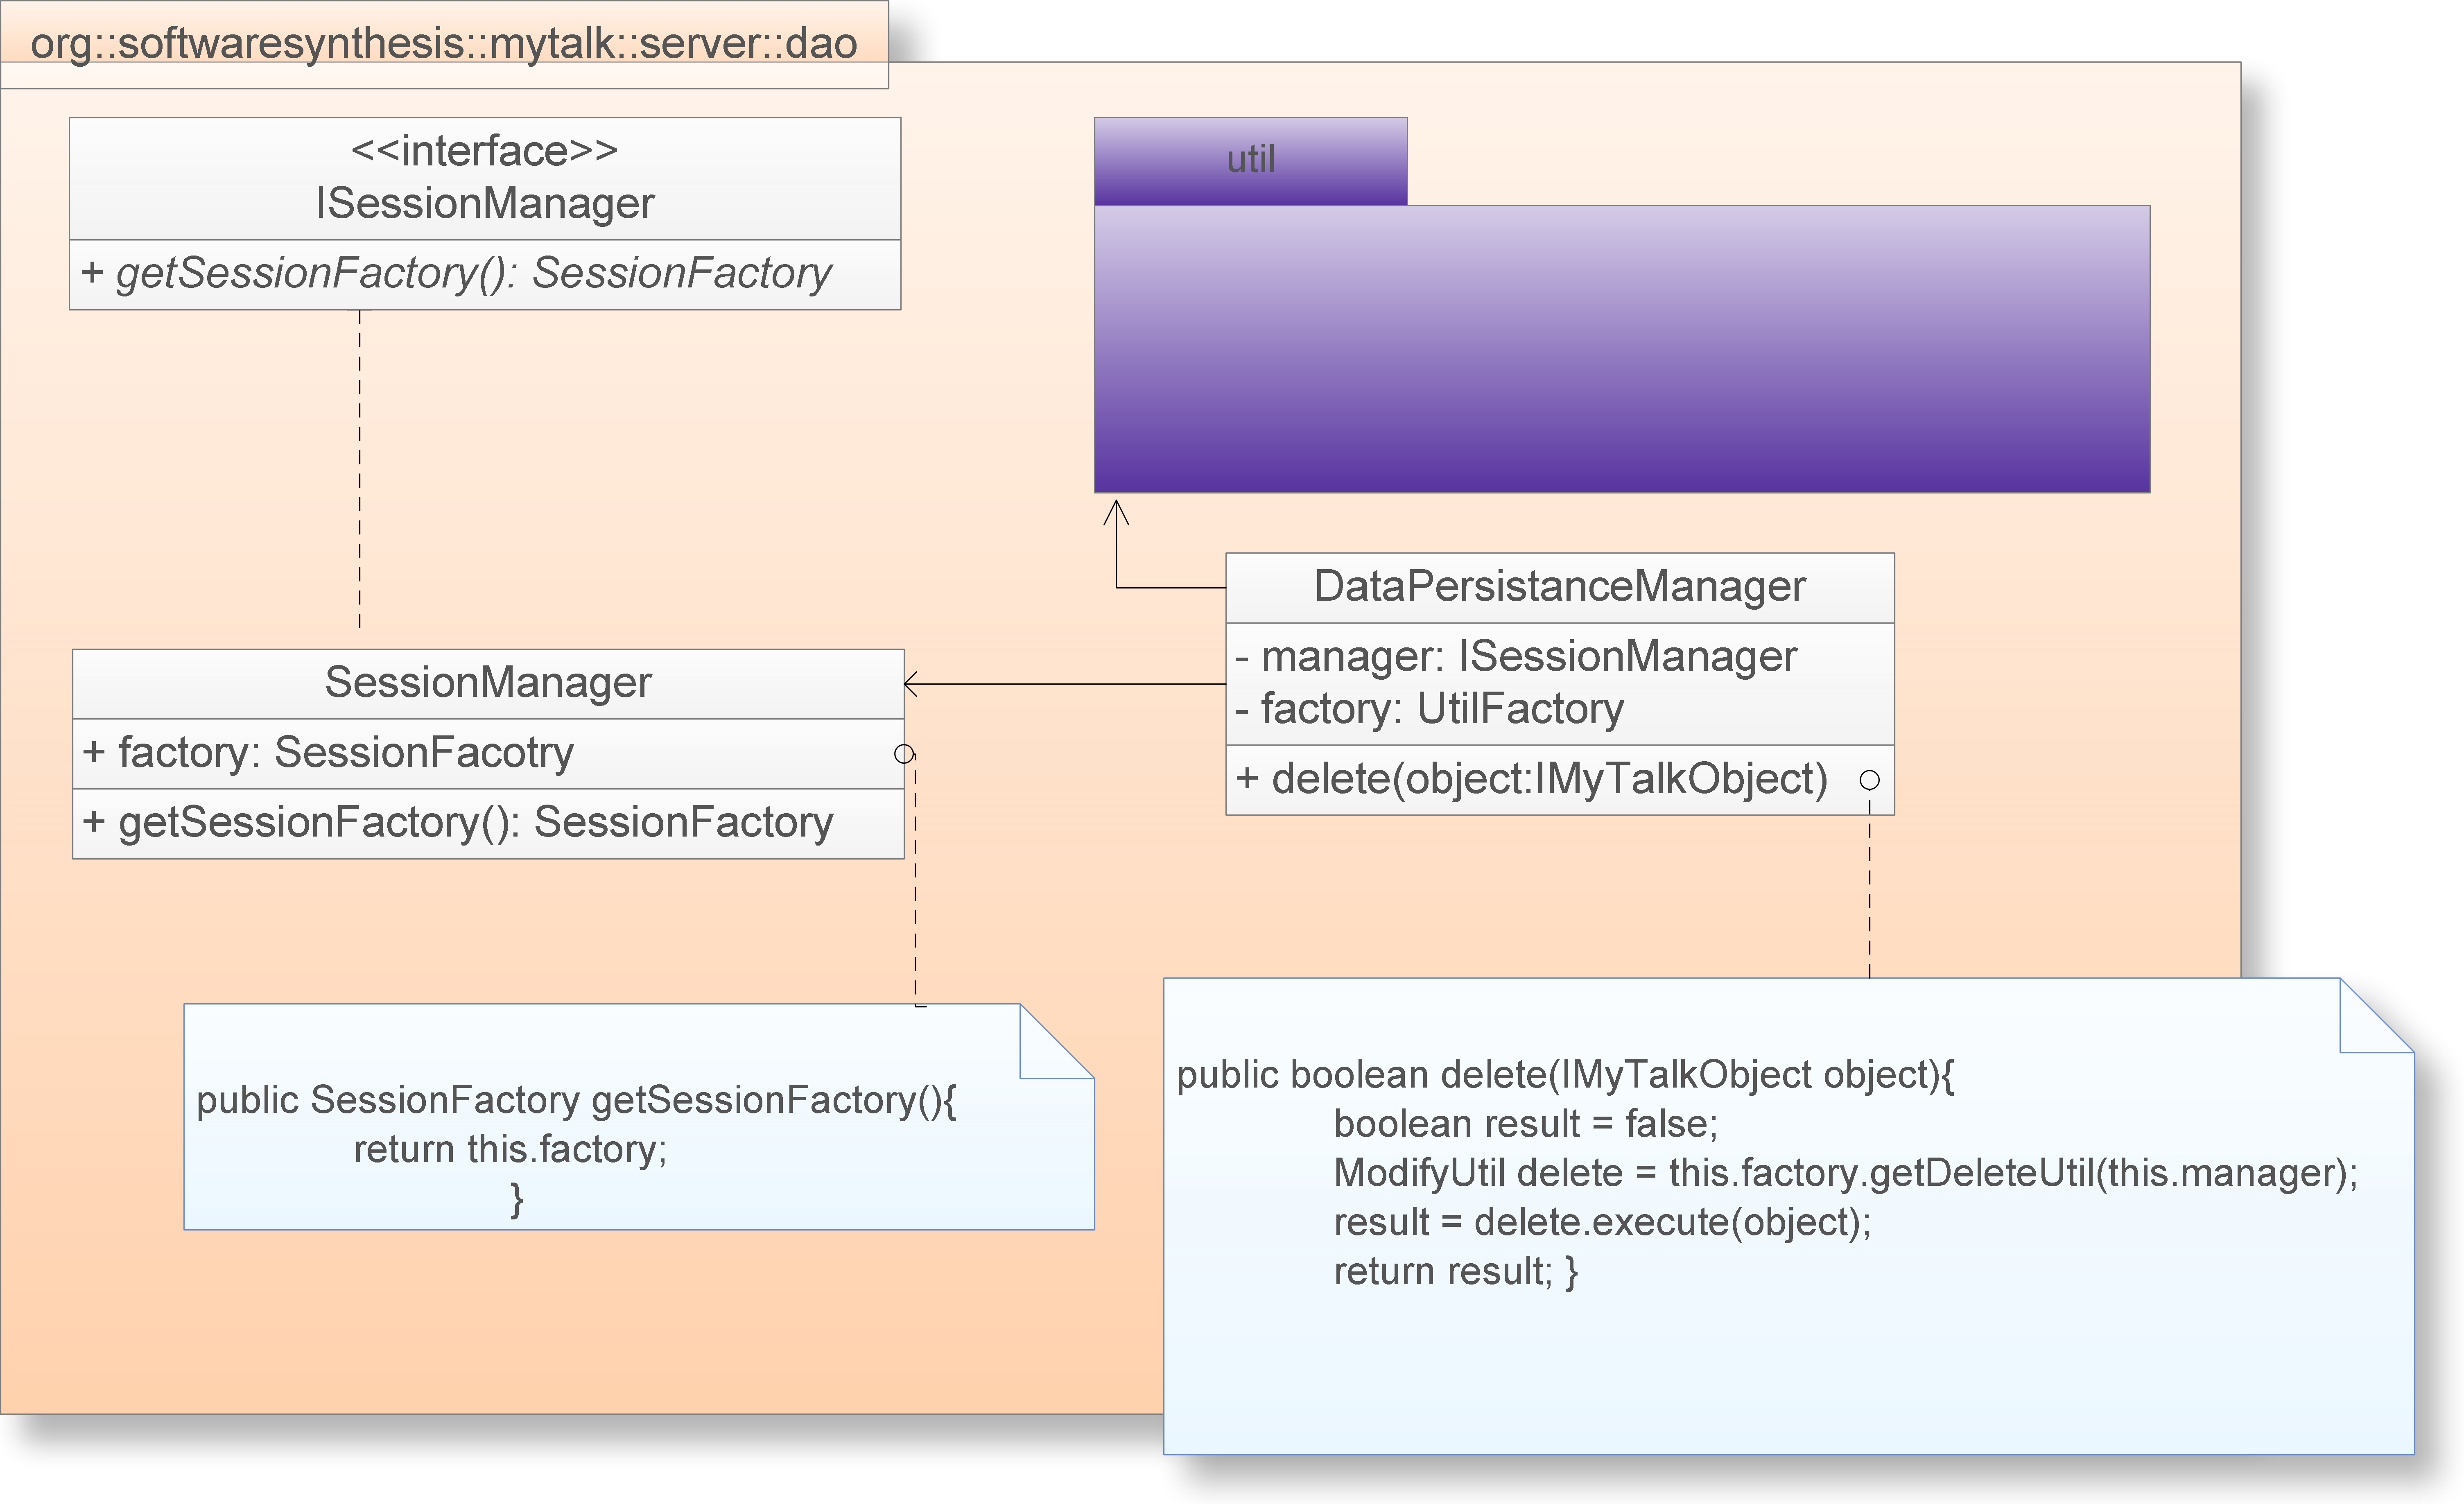
\includegraphics[width=\textwidth]{DDPDao}
\caption{Diagramma package server.dao}
\end{figure}

\classsection{ISessionManager}

\subsubsection*{Funzione}
Interfaccia rappresentante il comportamento di una generica classe adibita alla creazione e alla gestione delle sessioni \texttt{Hibernate} (di comunicazione con la base dati).

\subsubsection*{Relazioni d'uso}

Nessuna relazione evidenziata

\subsubsection*{Classi estese ed interfacce implementate}

Nessuna relazione evidenziata.


\subsubsection*{Metodi}
\begin{description}

	\item{\method{+ getSessionFactory(): SessionFactory}}\\
	Metodo usato per ottenere una sessione verso il database gestito mediante Hibernate.
	
\end{description}

\classsection{SessionManager}

\subsubsection*{Funzione}
Implementazione di \classname{ISessionManager}. Inizializza un'unica \inglese{factory} per le sessioni, utilizzate da Hibernate, per comunicare con il database.

\subsubsection*{Relazioni d'uso}

\begin{itemize}
	\item \classname{org.hibernate.SessionFactory}: necessaria per interrogare il database.
	\item \classname{org.hibernate.cfg.Configuration}: definisce i parametri necessari per la connessione con il database. Inoltre definisce i \textit{mapping} necessari tra le classi \inglese{transfer object} e le relative tabelle nel database.
\end{itemize}

\subsubsection*{Classi estese ed interfacce implementate}

\begin{itemize}
	\item \classname{dao.ISessionManager}: interfaccia d'implementazione del package \textit{dao} usata per definire il comportamento di un generico gestore Hibernate. Con gestore Hibernate intendiamo una classe in grado di creare delle sessioni con il database.
\end{itemize}

\subsubsection*{Attributi}

\begin{itemize}
	\item{\memberdata{\underline{-- instance: ISessionManager}}}\\
	Attributo usato per implementare il \inglese{pattern} singleton. Tale istanza verrà inizializzata tramite il metodo statico \method{getIstance()}, assicurando che l'attributo non sia già stato inizializzato in precedenza.
	\item{\memberdata{-- sessionFactory: SessionFactory}}\\
	Attributo contenente la \inglese{factory} delle sessioni verso il database.
\end{itemize}

\subsubsection*{Metodi}

\begin{description}
	\item{\method{-- SessionManager()}}\\
	Costruttore della classe, definito \inglese{private} in correlazione all'applicazione del \inglese{pattern} singleton. Il metodo si occupa dell'inizializzazione della \inglese{factory} per la creazione di sessioni di comunicazione verso la base dati.
	
	\item{\method{\underline{+ getInstance(): SessionManager}}}\\
	Metodo pubblico che ritorna l'istanza \memberdata{istance}. Il metodo controlla se \memberdata{istance} è già stata inizializzata, nel caso in cui non lo sia il metodo dovrà generare un istanza di \classname{SessionManager} richiamando il costruttore privato \method{SessionManager()} e assegnare il valore ritornato all'attributo \memberdata{istance}. Il programma termina restituendo \memberdata{istance}.
	
	\item{\method{\underline{+ getSessionFactory(): SessionFactory}}}\\
	Metodo che ritorna l'attributo \memberdata{sessionFactory}.
\end{description}

\classsection{DataPersistanceManager}

\subsubsection*{Funzione}
Classe che rappresenta un punto d'accesso al database del sistema. Implementata mediante le funzionalità di Hibernate, la classe permette di attuare operazioni \texttt{CRUD} sulle tabelle della base di dati.

\subsubsection*{Relazioni d'uso}

\begin{itemize}
	\item \texttt{org.softwaresynthesis.mytalk.server.IMyTalkObject};
	\item \texttt{org.softwaresynthesis.mytalk.server.abook.IGroup};
	\item \texttt{org.softwaresynthesis.mytalk.server.abook.IUserData};
	\item \texttt{org.softwaresynthesis.mytalk.server.dao.util.GetUtil};
	\item \texttt{org.softwaresynthesis.mytalk.server.dao.util.ModifyUtil};
	\item \texttt{org.softwaresynthesis.mytalk.server.dao.util.UtilFactory};
	\item \texttt{org.softwaresynthesis.mytalk.server.message.IMessage};
\end{itemize}

\subsubsection*{Classi estese ed interfacce implementate}

Nessuna relazione evidenziata.

\subsubsection*{Attributi}

\begin{itemize}
	\item{\memberdata{-- manager: ISessionManager}}\\
	Attributo usato per mantenere un riferimento alla singola istanza di SessionManagaer (estensione di \classname{ISessionManagaer}.
	\item{\memberdata{-- factory: UtilFactory}}\\
	Attributo usato per mantenere un riferimento ad un'istanza di UtilFactory, usata per l'esecuzione delle operazioni relative alla manipolazione dei dati.
\end{itemize}

\subsubsection*{Metodi}

\begin{description}
	\item{\method{+ DataPersistanceManager()}}\\
	Costruttore pubblico della classe. Richiama il costruttore \method{DataPersistanceManager(ISessionManager manager, UtilFactory factory)} passando come parametri \texttt{SessionMAnager.getIstance()} e una nuova istanza di \classname{UtilFactory}.
	
	\item{\method{\# DataPersistanceManager(manager: ISessionManager, factory: UtilFactory)}}\\
	Costruttore protetto della classe. Inizializza gli attributi della classe con i parametri d'ingresso.
	
	\item{\method{+ delete(object: IMyTalkObject): boolean}}\\
	Metodo per la manipolazione dei dati. Nello specifico permette di eseguire un operazione di eliminazione in una delle tabelle del database (tabella corrispondente all'oggetto object: \texttt{IMyTalkObject}). Il metodo definisce una variabile \texttt{result} di tipo \texttt{boolean} usata per evidenziare la buona riuscita o meno dell'operazione. Di default \texttt{result} è impostata a \texttt{false}. Il metodo crea un istanza di \classname{ModifyUtil} a partire da una chiamata \verb|this.factory.getDeleteUtil(this.manager)|. Quindi si salva in \texttt{result} il valore ritornato dall'operazione \verb|execute(object)| (dove \texttt{object}, parametro d'ingresso del metodo, rappresenta la tabella su cui eseguire l'operazione). \verb|execute(object)| è richiamata a partire dall'istanza \classname{ModifyUtil} creata in precedenza). Il metodo deve terminare ritornando il valore di \texttt{result}.
	
	
	\item{\method{+ insert(object: IMyTalkObject): boolean}}\\
	Metodo per la manipolazione dei dati. Nello specifico permette di eseguire un operazione di inserimento in una delle tabelle del database (tabella corrispondente all'oggetto \texttt{object}: {IMyTalkObject}). Il metodo definisce una variabile \texttt{result} di tipo \texttt{boolean} usata per evidenziare la buona riuscita o meno dell'operazione. Di default \texttt{result} è impostata a \texttt{false}. Il metodo crea un istanza di \classname{ModifyUtil} a partire da una chiamata \verb|this.factory.getInsertUtil(this.manager)|. Quindi si salva in result il valore ritornato dall'operazione \verb|execute(object)| (dove object, parametro d'ingresso del metodo, rappresenta la tabella su cui eseguire l'operazione). \verb|execute(object)| è richiamata a partire dall'istanza \classname{ModifyUtil} creata in precedenza). Il metodo deve terminare ritornando il valore di  \texttt{result}.
	
	\item{\method{+ update(object: IMyTalkObject): boolean}}\\
	Metodo per la manipolazione dei dati. Nello specifico permette di eseguire un operazione di modifica dei campi dati di una delle tabelle del database (tabella corrispondente all'oggetto object: IMyTalkObject). Il metodo definisce una variabile \texttt{result} di tipo \texttt{boolean} usata per evidenziare la buona riuscita o meno dell'operazione. Di default \texttt{result} è impostata a \texttt{false}. Il metodo crea un istanza di \classname{ModifyUtil} a partire da una chiamata \verb|this.factory.getUpdateUtil(this.manager)|. Quindi si salva in \texttt{result} il valore ritornato dall'operazione \verb|execute(object)| (dove \texttt{object}, parametro d'ingresso del metodo, rappresenta la tabella su cui eseguire l'operazione). \verb|execute(object)| è richiamata a partire dall'istanza \classname{ModifyUtil} creata in precedenza). Il metodo deve terminare ritornando il valore di \texttt{result}.
	
	\item{\method{+ getGroup(id: Long): IGroup}}\\
	Metodo usato per l'esecuzione di una query SQL atta ad garantire la restituzione dei dati inerenti il gruppo avente come \inglese{primary key} il valore contenuto in \texttt{id}. Il metodo definisce un istanza di \classname{GetUtil} mediante una chiamata \verb|this.factory.getGroupUtil(this.manager)|. Quindi definisce un oggetto \classname{IGroup} denominato \texttt{result}. Successivamente si definisce una lista \texttt{List<IMyTalkObject>}, da usare per memorizzare temporaneamente i dati ottenuti dall'esecuzione della query:\\
	
	\verb|from Groups as g where g.id = VALORE_id|\\
	
	Tale operazione si ottiene con l'istruzione \verb|select.execute(query)|. Quindi si controlla se la lista cosi popolata contiene almeno un elemento (che per come è stata progettata la query, ossia un interrogazione su chiave primaria, deve essere al più uno). Nel caso si imposta \texttt{result} con una chiamata a metodo \texttt{get()} richiamato dalla lista usata. Il metodo termina restituendo \texttt{result}.
	
		\item{\method{+ getGroup(owner: IUserData): List<IGroup>}}\\
	Metodo usato per l'esecuzione di una query SQL atta ad garantire la restituzione dei gruppi aventi come possessore l'utente \textit{owner}. Il metodo definisce un istanza di \classname{GetUtil} mediante una chiamata \verb|this.factory.getGroupUtil(this.manager)|. Quindi definisce un oggetto \classname{IGroup} denominato \texttt{result}. Successivamente si definisce una lista \texttt{List<IMyTalkObject>}, da usare per memorizzare temporaneamente i dati ottenuti dall'esecuzione della query:\\
	
	\verb|from Groups as g where g.owner.id = VALORE_owner|\\
	
	Tale operazione si ottiene con l'istruzione \verb|select.execute(query)|. Quindi si controlla se la lista cosi popolata contiene almeno un elemento. Nel caso si imposta \texttt{result} uguale alla lista usata. Il metodo termina restituendo \texttt{result}.
	
			\item{\method{+ getGroup(owner: IUserData, name: String): List<IGroup>}}\\
	Metodo usato per l'esecuzione di una query SQL atta ad garantire la restituzione dei gruppi aventi come possessore l'utente \textit{owner} e nome del gruppo uguale al valore contenuto in name. Il metodo definisce un istanza di \classname{GetUtil} mediante una chiamata \verb|this.factory.getGroupUtil(this.manager)|. Quindi definisce un oggetto \classname{IGroup} denominato \texttt{result}. Successivamente si definisce una lista \texttt{List<IMyTalkObject>}, da usare per memorizzare temporaneamente i dati ottenuti dall'esecuzione della query:\\
	
	\verb|from Groups as g where g.owner.id = VALORE_owner and g.name = VALORE_name |\\
	
	Tale operazione si ottiene con l'istruzione \verb|select.execute(query)|. Quindi si controlla se la lista cosi popolata contiene almeno un elemento. Nel caso si imposta \texttt{result} uguale alla lista usata. Il metodo termina restituendo \texttt{result}.
	
	\item{\method{+ getMessageNewKey(): Long}}\\
	Metodo usato per l'esecuzione di una query SQL atta ad garantire la restituzione della più alta chiave primaria usata nella tabella \texttt{message}. Il metodo restituirà tale valore maggiorato di 1. Il metodo definisce un istanza di \classname{GetUtil} mediante una chiamata \verb|this.factory.getGenericUtil(this.manager)|. Quindi definisce un oggetto \classname{Long} denominato \texttt{result}. Successivamente si definisce un \texttt{long} nominato \texttt{id}, da usare per memorizzare temporaneamente il dato ottenuto dall'esecuzione della query:\\
	
	\verb|max(message.id) from Message|\\
	
	Tale operazione si ottiene con l'istruzione \verb|select.execute(query)|. Quindi si controlla se la variabile \texttt{id} contiene almeno un elemento. Nel caso si imposta \texttt{result} uguale alla uguale al contenuto di \texttt{id} + 1. Il metodo termina restituendo \texttt{result}.
	
	\item{\method{+ getMessage(id: Long): IMessage}}\\
	Metodo usato per l'esecuzione di una query SQL atta a garantire la restituzione dei dati inerenti il messaggio avente come \textit{primary key} il valore contenuto in \texttt{id}. Il metodo definisce un istanza di \classname{GetUtil} mediante una chiamata \verb|this.factory.getGenericUtil(this.manager)|. Quindi definisce un oggetto \classname{IGroup} denominato \texttt{result}. Successivamente si definisce una lista \texttt{List<IMyTalkObject>}, da usare per memorizzare temporaneamente i dati ottenuti dall'esecuzione della query:\\
	
	\verb|from Message as m where m.id = VALORE_id|\\
	
	Tale operazione si ottiene con l'istruzione \verb|select.execute(query)|. Quindi si controlla se la lista cosi popolata contiene almeno un elemento (che per come è stata progettata la query, ossia un interrogazione su chiave primaria, deve essere al più uno). Nel caso si imposta \texttt{result} con una chiamata a metodo \texttt{get()} richiamato dalla lista usata. Il metodo termina restituendo \texttt{result}.
	
		\item{\method{+ getMessages(receiver: IUserData): List<IMessages>}}\\
	Metodo usato per l'esecuzione di una query SQL atta ad garantire la restituzione dei messaggi aventi come ricevente l'utente \textit{receiver}. Il metodo definisce un istanza di \classname{GetUtil} mediante una chiamata \verb|this.factory.getGenericUtil(this.manager)|. Quindi definisce un oggetto \classname{IMessages} denominato result. Successivamente si definisce una lista \texttt{List<IMyTalkObject>}, da usare per memorizzare temporaneamente i dati ottenuti dall'esecuzione della query:\\
	
	\verb|from Message as m where m.receiver.id = VALORE_receiver|\\
	
	Tale operazione si ottiene con l'istruzione \verb|select.execute(query)|. Quindi si controlla se la lista cosi popolata contiene almeno un elemento. Nel caso si imposta \texttt{result} uguale alla lista usata. Il metodo termina restituendo \texttt{result}.	
	
	\item{\method{+ getUserData(mail: String): IUserData}}\\
	Metodo usato per l'esecuzione di una query SQL atta a garantire la restituzione dei dati inerenti l'utente avente come indirizzo mail il valore contenuto in \texttt{mail}. Il metodo definisce un istanza di \classname{GetUtil} mediante una chiamata \verb|this.factory.getUserDataUtil(this.manager)|. Quindi definisce un oggetto \classname{IUserData} denominato result. Successivamente si definisce una lista \texttt{List<IMyTalkObject>}, da usare per memorizzare temporaneamente i dati ottenuti dall'esecuzione della query:\\
	
	\verb|from UserData as u where u.mail = VALORE_mail|\\
	
	Tale operazione si ottiene con l'istruzione \verb|select.execute(query)|. Quindi si controlla se la lista cosi popolata contiene almeno un elemento (che per come è stata progettata la query, ossia un interrogazione su chiave primaria, deve essere al più uno). Nel caso si imposta \texttt{result} con una chiamata a metodo \texttt{get()} richiamato dalla lista usata. Il metodo termina restituendo \texttt{result}.	
	
	\item{\method{+ getUserData(id: Long): IUserData}}\\
	Metodo usato per l'esecuzione di una query SQL atta a garantire la restituzione dei dati inerenti l'utente avente come chiave primaria il valore contenuto in \texttt{id}. Il metodo definisce un istanza di \classname{GetUtil} mediante una chiamata \verb|this.factory.getUserDataUtil(this.manager)|. Quindi definisce un oggetto \classname{IUserData} denominato \texttt{result}. Successivamente si definisce una lista \texttt{List<IMyTalkObject>}, da usare per memorizzare temporaneamente i dati ottenuti dall'esecuzione della query:\\
	
	\verb|from UserData as u where u.id = VALORE_id|\\
	
	Tale operazione si ottiene con l'istruzione \verb|select.execute(query)|. Quindi si controlla se la lista cosi popolata contiene almeno un elemento (che per come è stata progettata la query, ossia un interrogazione su chiave primaria, deve essere al più uno). Nel caso si imposta \texttt{result} con una chiamata a metodo \texttt{get()} richiamato dalla lista usata. Il metodo termina restituendo \texttt{result}.
	
	\item{\method{+ getUserDatas(mail: String, name: String, surname: String): List<IUserData>}}\\
	Metodo usato per l'esecuzione di una query SQL atta ad garantire la restituzione degli utenti aventi come valore dei campi omonimi ai parametri del metodo, il valore di quest'ultimi. Il metodo definisce un istanza di \classname{GetUtil} mediante una chiamata \\ \verb|this.factory.getUserDataUtil(this.manager)|. Quindi definisce un oggetto \classname{IUserData} denominato \texttt{result}. Successivamente si definisce una lista \texttt{List<IMyTalkObject>}, da usare per memorizzare temporaneamente i dati ottenuti dall'esecuzione della query:\\
	
	\verb|from UserData as u where u.mail like %VALORE_receiver%|\\
	\verb|or u.name like %VALORE_name% or u.surname like %VALORE_surname%|\\
	
	Tale operazione si ottiene con l'istruzione \verb|select.execute(query)|. Quindi si controlla se la lista cosi popolata contiene almeno un elemento. Nel caso si imposta \texttt{result} uguale alla lista usata. Il metodo termina restituendo \texttt{result}.
	
		\item{\method{+ getCall(id: Long): ICall}}\\
	Metodo usato per l'esecuzione di una query SQL atta a garantire la restituzione dei dati inerenti ad una chiamata avente come chiave primaria il valore contenuto in \texttt{id}. Il metodo definisce un istanza di \classname{GetUtil} mediante una chiamata \verb|this.factory.getCallUtil(this.manager)|. Quindi definisce un oggetto \classname{ICall} denominato \texttt{result}. Successivamente si definisce una lista \texttt{List<IMyTalkObject>}, da usare per memorizzare temporaneamente i dati ottenuti dall'esecuzione della query:\\
	
	\verb|from Call as c where c.id = VALORE_id|\\
	
	Tale operazione si ottiene con l'istruzione \verb|select.execute(query)|. Quindi si controlla se la lista cosi popolata contiene almeno un elemento (che per come è stata progettata la query, ossia un interrogazione su chiave primaria, deve essere al più uno). Nel caso si imposta \texttt{result} con una chiamata a metodo \texttt{get()} richiamato dalla lista usata. Il metodo termina restituendo \texttt{result}.
	
\end{description}

\subsection{Package \texttt{org.softwaresynthesis.mytalk.server.dao.util}}\label{sec:daoUtil}

\begin{figure}[H]
  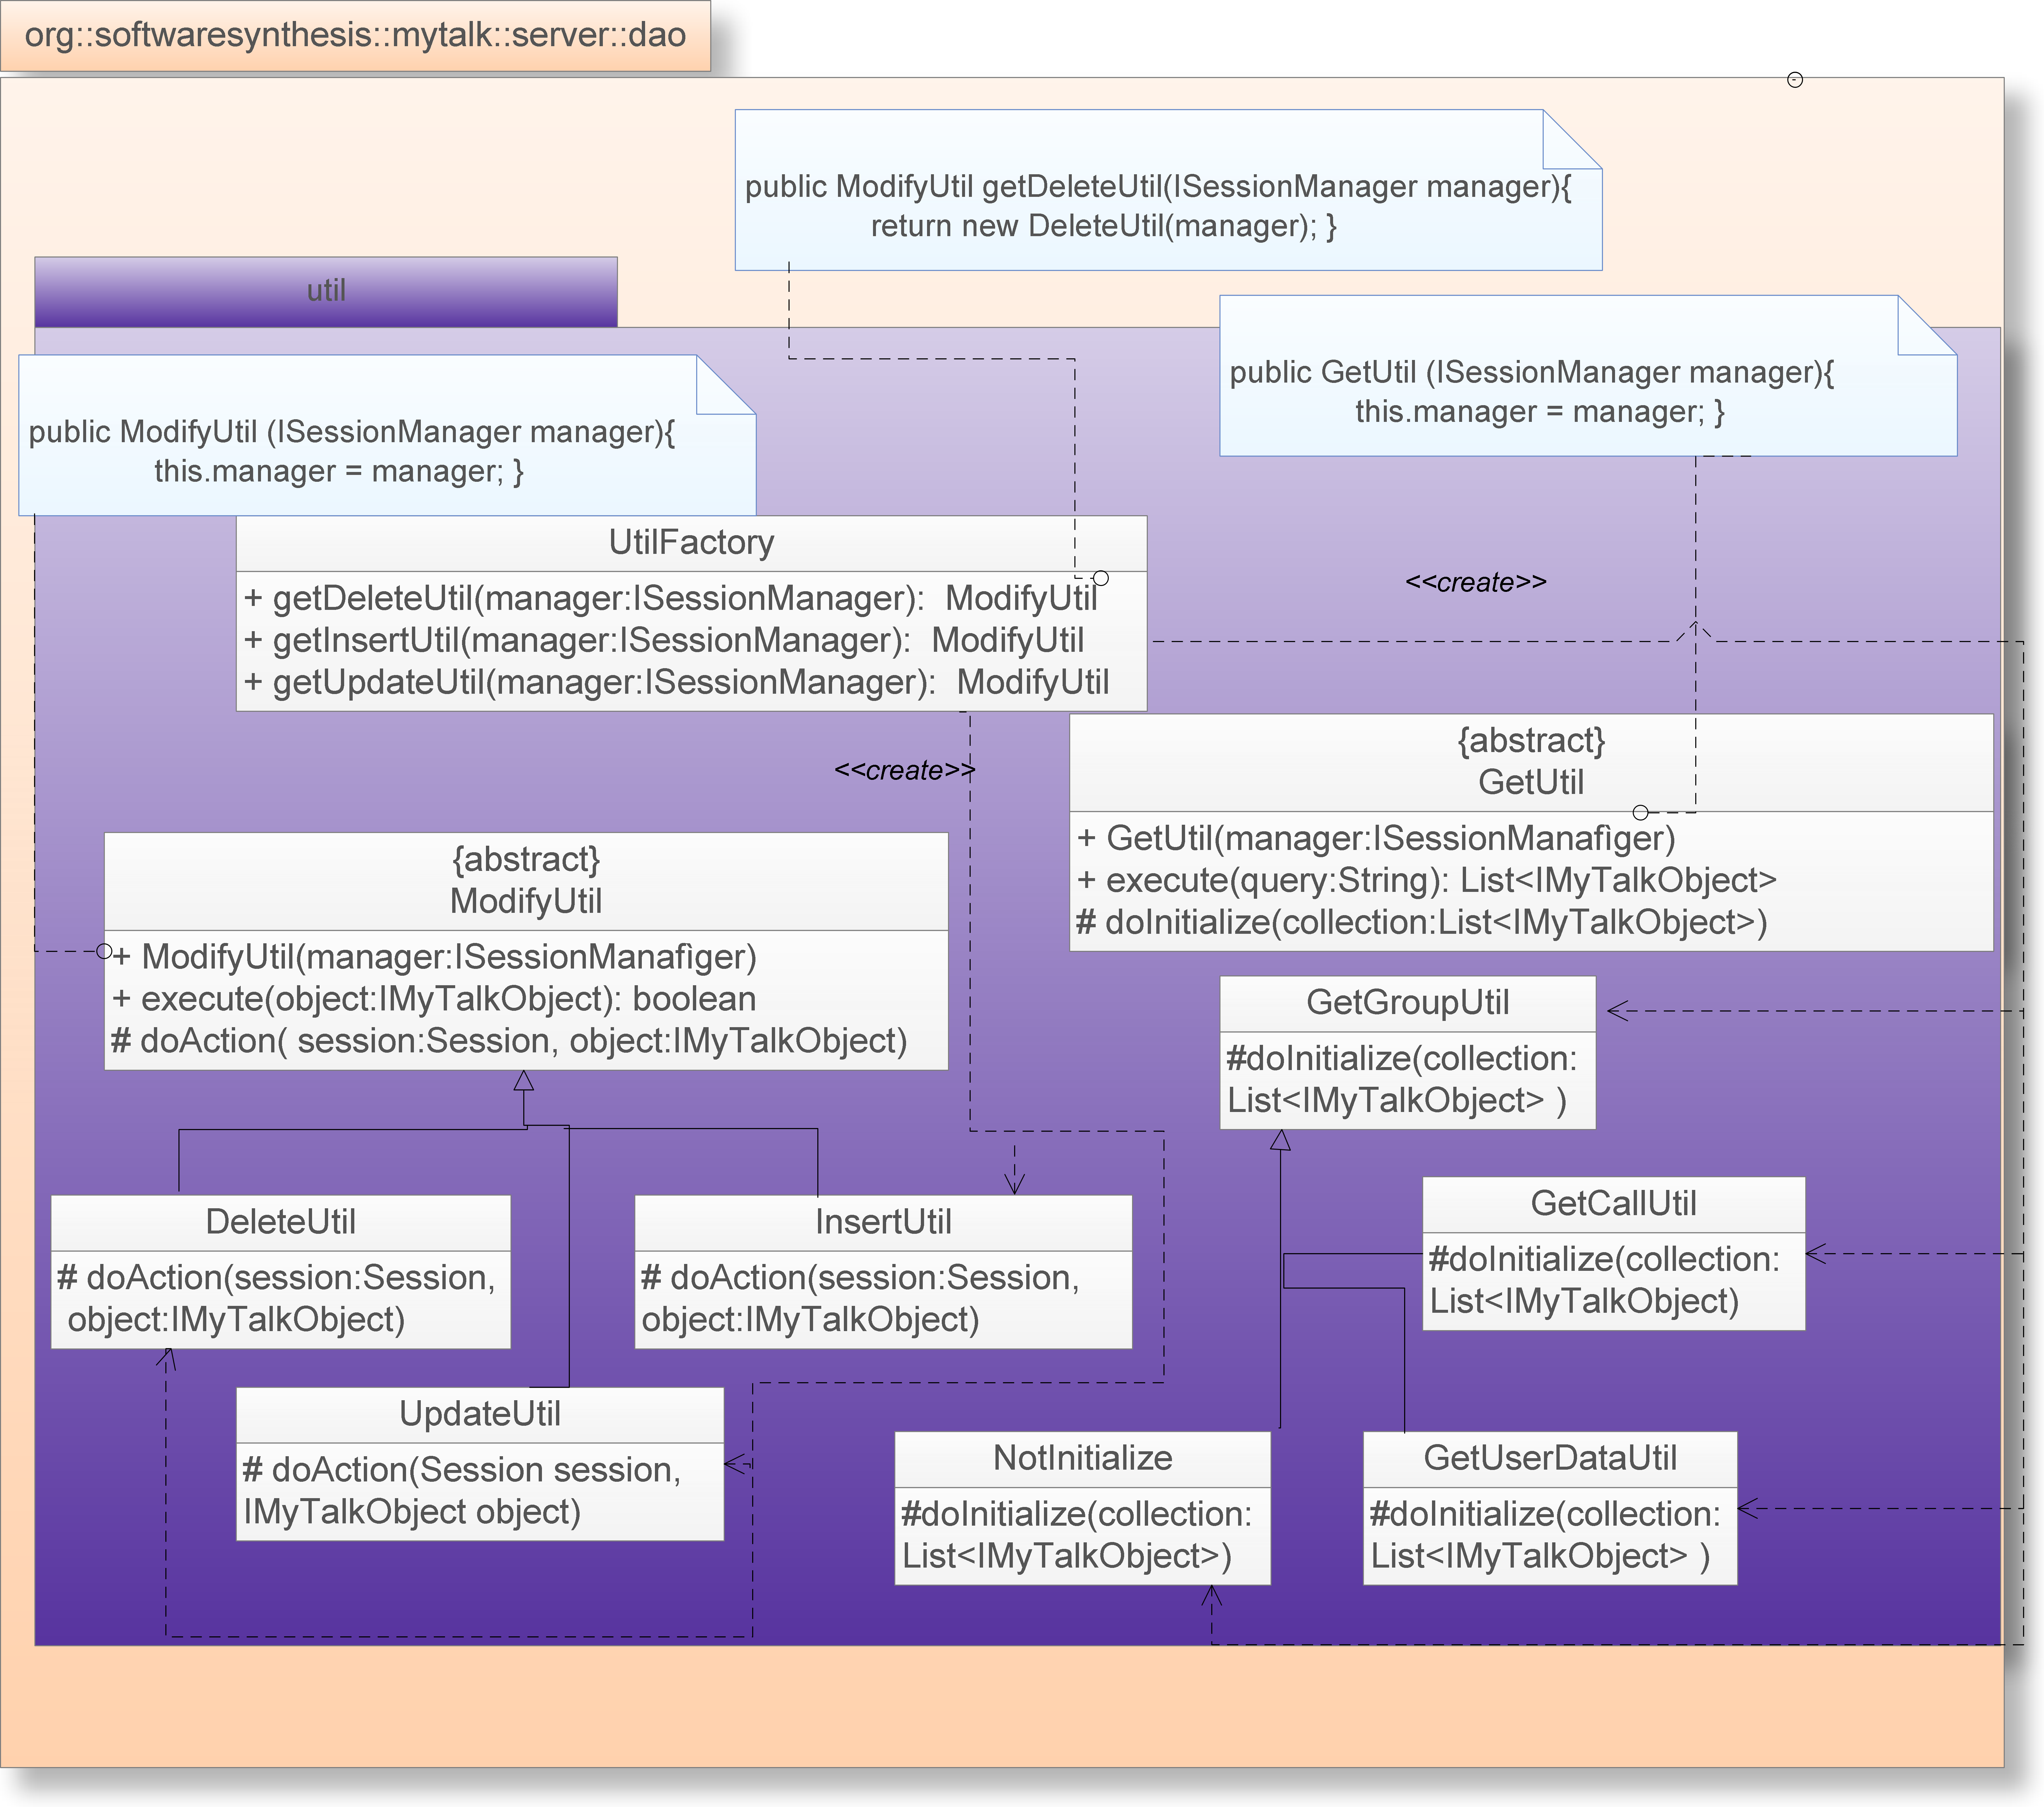
\includegraphics[width=\textwidth]{DDPDaoUtil}
\caption{Diagramma package server.dao.util}
\end{figure}

\classsection{UtilFactory}

\subsubsection*{Funzione}
Classe usata per la creazione delle classi di manipolazione del database.

\subsubsection*{Relazioni d'uso}

\begin{itemize}
		\item{org.softwaresynthesis.mytalk.server.dao.ISessionManager}: usata per definire un riferimento con il sistema centrale per la gestione del database.
\end{itemize}

\subsubsection*{Classi estese ed interfacce implementate}

Nessuna relazione evidenziata.

\subsubsection*{Attributi}

Nessun attributo evidenziare.

\subsubsection*{Metodi}

\begin{description}
	\item{\method{+ getDeleteUtil(manager: ISessionManager): ModifyUtil}}\\
	Metodo usato per ritornare un \inglese{utility} per la cancellazione di un record. Il metodo restituisce \verb|new DeleteUtil(manager)|.
	
	\item{\method{+ getInsertUtil(manager: ISessionManager): ModifyUtil}}\\
	Metodo usato per ritornare una \inglese{utility} per l'inserimento di un record. Il metodo restituisce \verb|new InsertUtil(manager)|.
	
	\item{\method{+ getUpdateUtil(manager: ISessionManager): ModifyUtil}}\\
	Metodo usato per ritornare una \inglese{utility} per l'aggiornamento di un record. Il metodo restituisce \verb|new UpdateUtil(manager)|.
	
	\item{\method{+ getCallUtil(manager: ISessionManager): GetUtil}}\\
	Metodo usato per ritornare una \inglese{utility} per inizializzare correttamente oggetti rappresentanti una chiamata. Il metodo restituisce \verb|new GetCallUtil(manager)|.	
	
	\item{\method{+ getGroupUtil(manager: ISessionManager): GetUtil}}
		Metodo usato per ritornare una \inglese{utility} per inizializzare correttamente oggetti rappresentanti gruppi di utenti. Il metodo restituisce \verb|new GetGroupUtil(manager)|.	
	
	\item{\method{+ getUserDataUtil(manager: ISessionManager): GetUtil}}\\
		Metodo usato per ritornare una \inglese{utility} per inizializzare correttamente oggetti rappresentanti utenti del sistema. Il metodo restituisce \verb|new GetUserDataUtil(manager)|.	

	\item{\method{+ getGenericUtil(manager: ISessionManager): GetUtil}}\\
		Metodo usato per ritornare una \inglese{utility} per estrarre dal database oggetti che non contengono campi dati di tipo \texttt{collezione} che devono essere inizializzate. Il metodo restituisce \verb|new NotInitialize(manager)|.	
		
\end{description}		

\classsection{ModifyUtil}

\subsubsection*{Funzione}
Classe astratta per definire il comportamento generico di una classe per la manipolazione del database. La classe costituisce un implementazione del \textit{template method}, poiché definisce un iter per l'esecuzione di un algoritmo di modifica, lasciando alle classi figlie il compito di ridefinire il metodo \method{doAction()}.

\subsubsection*{Relazioni d'uso}

\begin{itemize}
		\item \texttt{org.hibernate.Session};
		\item \texttt{org.hibernate.SessionFactory};
		\item \texttt{org.hibernate.Transaction};
		\item \texttt{org.softwaresynthesis.mytalk.server.IMyTalkObject};
		\item \texttt{org.softwaresynthesis.mytalk.server.dao.ISessionManager};
\end{itemize}

\subsubsection*{Classi estese ed interfacce implementate}

Nessuna relazione evidenziata.

\subsubsection*{Attributi}

\begin{itemize}
	\item{\memberdata{\underline{-- manager: ISessionManager}}}\\
	Attributo usato per comunicare con la classe rappresentate il ''cuore'' del sistema di gestione del database.
\end{itemize}

\subsubsection*{Metodi}

\begin{description}
	\item{\method{+ ModifyUtil(manager: ISessionManager)}}\\
	Costruttore pubblico della classe, usato per inizializzare \memberdata{manager} con il parametro d'ingresso del metodo.
	
	\item{\method{+ execute(object: IMyTalkObject): boolean}}\\
	Metodo che definisce l'iter per l'esecuzione dell'operazione di manipolazione del database. Il metodo definisce quelle procedure comuni a tutte le operazioni di modifica. Inizialmente il metodo definisce i seguenti oggetti:
	\begin{itemize}
		\item boolean result = false;
		\item Session session = null;
		\item SessionFactory factory = null;
		\item Transaction transaction = null;
	\end{itemize}
	
Quindi viene definito un blocco try-catch. Nel blocco try, si salva in \texttt{factory} un riferimento a \classname{SessionManager}. Quindi in \texttt{session} si riporta la sessione ottenuta da una chiamata \verb|factory.openSession()|. Si definisce l'apertura di una transizione \texttt{transaction} mediante una chiamata \verb|session.beginTransaction()|. Il metodo procede eseguendo il metodo \method{doAction()} passando come parametro d'ingresso \texttt{session} e \texttt{object}. Si esegue il \texttt{commit} sulla transizione e si imposta \texttt{result} a \texttt{true}. Nel blocco catch si esegue un'operazione di \inglese{rollback} e si imposta \texttt{result} a \texttt{false}.

Il metodo termina chiudendo la sessione e ritornando il contenuto di \texttt{result}.

	\item{\method{+ \{abstract\} doAction(session: ISessionManager, object: IMyTalkObject): void}}\\
	Metodo astratto non definito in questa classe. Le classi figlie di \classname{ModifyUtil} ridefiniranno questo metodo.

\end{description}

\classsection{InsertUtil}

\subsubsection*{Funzione}
Classe figlia di \classname{ModifyUtil}. Ridefinisce il metodo \method{doAction} per eseguire un operazione di \texttt{insert} in una tabella del database.

\subsubsection*{Relazioni d'uso}

\begin{itemize}
		\item \texttt{org.hibernate.Session};
		\item \texttt{org.softwaresynthesis.mytalk.server.IMyTalkObject};
		\item \texttt{org.softwaresynthesis.mytalk.server.dao.ISessionManager};
\end{itemize}

\subsubsection*{Classi estese ed interfacce implementate}

\begin{itemize}
	\item \classname{dao.util.ModifyUtil}: classe astratta estesa.
\end{itemize}

\subsubsection*{Attributi}

Nessun attributo evidenziato.

\subsubsection*{Metodi}

\begin{description}
	\item{\method{+ InsertUtil(manager: ISessionManager)}}\\
	Costruttore pubblico della classe, usato per inizializzare \memberdata{manager} con il parametro d'ingresso del metodo. Per farlo richiama il costruttore della classe padre.

	\item{\method{+ \{final\} doAction(session: ISessionManager, object: IMyTalkObject): void}}\\
	Metodo usato per eseguire un operazione di insert nel database. Il metodo esegue l'unica operazione \verb|session.save(object)|.

\end{description}

\classsection{DeleteUtil}

\subsubsection*{Funzione}
Classe figlia di \classname{ModifyUtil}. Ridefinisce il metodo \method{doAction} per eseguire un operazione di \texttt{delete} in una tabella del database.

\subsubsection*{Relazioni d'uso}

\begin{itemize}
		\item \texttt{org.hibernate.Session};
		\item \texttt{org.softwaresynthesis.mytalk.server.IMyTalkObject};
		\item \texttt{org.softwaresynthesis.mytalk.server.dao.ISessionManager};
\end{itemize}

\subsubsection*{Classi estese ed interfacce implementate}

\begin{itemize}
	\item \classname{dao.util.ModifyUtil}: classe astratta estesa.
\end{itemize}

\subsubsection*{Attributi}

Nessun attributo evidenziato.

\subsubsection*{Metodi}

\begin{description}
	\item{\method{+ DeleteUtil(manager: ISessionManager)}}\\
	Costruttore pubblico della classe, usato per inizializzare \memberdata{manager} con il parametro d'ingresso del metodo. Per farlo richiama il costruttore della classe padre.

	\item{\method{+ \{final\} doAction(session: ISessionManager, object: IMyTalkObject): void}}\\
	Metodo usato per eseguire un operazione di delete nel database. Il metodo esegue l'unica operazione \verb|session.delete(object)|.

\end{description}

\classsection{UpdateUtil}

\subsubsection*{Funzione}
Classe figlia di \classname{ModifyUtil}. Ridefinisce il metodo \method{doAction} per eseguire un operazione di aggiornamento (intesa come modifica del valore di alcuni campi dati) in una tabella del database.

\subsubsection*{Relazioni d'uso}

\begin{itemize}
		\item \texttt{org.hibernate.Session};
		\item \texttt{org.softwaresynthesis.mytalk.server.IMyTalkObject};
		\item \texttt{org.softwaresynthesis.mytalk.server.dao.ISessionManager};
\end{itemize}

\subsubsection*{Classi estese ed interfacce implementate}

\begin{itemize}
	\item \classname{dao.util.ModifyUtil}: classe astratta estesa.
\end{itemize}

\subsubsection*{Attributi}

Nessun attributo evidenziato.

\subsubsection*{Metodi}

\begin{description}
	\item{\method{+ UpdateUtil(manager: ISessionManager)}}\\
	Costruttore pubblico della classe, usato per inizializzare \memberdata{manager} con il parametro d'ingresso del metodo. Per farlo richiama il costruttore della classe padre.

	\item{\method{+ \{final\} doAction(session: ISessionManager, object: IMyTalkObject): void}}\\
	Metodo usato per eseguire un operazione di \inglese{update} nel database. Il metodo esegue l'unica operazione \verb|session.update(object)|.

\end{description}

\classsection{GetUtil}

\subsubsection*{Funzione}
Classe astratta per definire il comportamento generico di una classe per l'esecuzione di ''interrogazioni'' (query di tipo \texttt{select}) al database. La classe costituisce un implementazione del \textit{template method}, poiché definisce un iter per l'esecuzione di un algoritmo, lasciando alle classi figlie il compito di ridefinire il metodo \method{doInitialize()}.

\subsubsection*{Relazioni d'uso}

\begin{itemize}
		\item \texttt{java.util.List};
		\item \texttt{org.hibernate.Query};
		\item \texttt{org.hibernate.Session};
		\item \texttt{org.hibernate.SessionFactory};
		\item \texttt{org.hibernate.Transaction};
		\item \texttt{org.softwaresynthesis.mytalk.server.IMyTalkObject};
		\item \texttt{org.softwaresynthesis.mytalk.server.dao.ISessionManager};
\end{itemize}

\subsubsection*{Classi estese ed interfacce implementate}

Nessuna relazione evidenziata.

\subsubsection*{Attributi}

\begin{itemize}
	\item{\memberdata{\underline{-- manager: ISessionManager}}}\\
	Attributo usato per comunicare con la classe rappresentate il ''cuore'' del sistema di gestione del database.
\end{itemize}

\subsubsection*{Metodi}

\begin{description}
	\item{\method{+ GetUtil(manager: ISessionManager)}}\\
	Costruttore pubblico della classe, usato per inizializzare \memberdata{manager} con il parametro d'ingresso del metodo.
	
	\item{\method{+ execute(query: String): List<IMyTalkObject>}}\\
	Metodo che definisce l'iter per l'esecuzione dell'operazione d'interrogazione del database,  definisce quelle procedure comuni a tutte le operazioni di lettura dei dati. Inizialmente il metodo definisce i seguenti oggetti:
	\begin{itemize}
		\item Query hqlQuery = null;
		\item List<IMyTalkObject> collection = null;
		\item Session session = null;
		\item SessionFactory factory = null;
		\item Transaction transaction = null;
	\end{itemize}
	
Quindi viene definito un blocco try-catch. Nel blocco try, si salva in \textit{factory} un riferimento a \classname{SessionManager}. Quindi in \texttt{session} si riporta la sessione ottenuta da una chiamata \verb|factory.openSession()|. Si definisce la query d'interrogazione mediante una chiamata \verb|session.createQuery(query)|. Si definisce l'apertura di una transizione \textit{transaction} mediante una chiamata \verb|session.beginTransaction()|. Il metodo procede prima impostando \texttt{collection} a \verb|(List<IMyTalkObject>)hqlQuery.list();|, e poi eseguendo il metodo \method{doInitialize()} passando come parametro d'ingresso \texttt{collection}. Si esegue il \textit{commit} sulla transizione e si imposta \texttt{result} a \texttt{true}. Nel blocco catch si esegue un'operazione di \textit{rollback} e si imposta \texttt{collection} a \texttt{null}.

Il metodo termina chiudendo la sessione e ritornando il contenuto di \texttt{collection}.

	\item{\method{+ uniqueResult(query: String): Long}}\\
	Metodo che definisce l'iter per l'esecuzione dell'operazione d'interrogazione del database (quelle che prevedono un unico risultato). Il metodo definisce quelle procedure comuni a tutte le operazioni di lettura dei dati. Inizialmente il metodo definisce i seguenti oggetti:
	\begin{itemize}
		\item Query hqlQuery = null;
		\item Long result = null;
		\item Session session = null;
		\item SessionFactory factory = null;
		\item Transaction transaction = null;
	\end{itemize}
	
Quindi viene definito un blocco try-catch. Nel blocco try, si salva in factory un riferimento a \classname{SessionManager}. Quindi in \textit{session} si riporta la sessione ottenuta da una chiamata \verb|factory.openSession()|. Si definisce la query d'interrogazione mediante una chiamata \verb|session.createQuery(query)|. Si definisce l'apertura di una transizione \texttt{transaction} mediante una chiamata \verb|session.beginTransaction()|. Il metodo procede prima impostando \texttt{result} a \verb|(Long)hqlQuery.uniqueResult()|, e poi eseguendo l'operazione di \textit{commit} a partire dall'oggetto \texttt{transaction}. Nel blocco catch si esegue un'operazione di \textit{rollback} e si imposta \texttt{result} a \inglese{null}.

Il metodo termina chiudendo la sessione e ritornando il contenuto di \texttt{result}.

	\item{\method{+ \{abstract\} doInitialize(collection: List<IMyTalkObject>): void}}\\
	Metodo astratto non definito in questa classe. Le classi figlie di \classname{GetUtil} ridefiniranno questo metodo.

\end{description}

\classsection{GetCallUtil}

\subsubsection*{Funzione}
Classe figlia di \classname{GetUtil}. Rappresenta l'operazione necessaria per ottenere le chiamate registrate nel database.

\subsubsection*{Relazioni d'uso}

\begin{itemize}
		\item \texttt{java.util.Iterator};
		\item \texttt{import java.util.List};
		\item \texttt{import org.hibernate.Hibernate};
		\item \texttt{org.hibernate.Session};
		\item \texttt{org.softwaresynthesis.mytalk.server.IMyTalkObject};
		\item \texttt{org.softwaresynthesis.mytalk.server.dao.ISessionManager};
\end{itemize}

\subsubsection*{Classi estese ed interfacce implementate}

\begin{itemize}
	\item \classname{dao.util.GetUtil}: classe astratta estesa.
\end{itemize}

\subsubsection*{Attributi}

Nessun attributo evidenziato.

\subsubsection*{Metodi}

\begin{description}
	\item{\method{+ GetCallUtil(manager: ISessionManager)}}\\
	Costruttore pubblico della classe, usato per inizializzare \memberdata{manager} con il parametro d'ingresso del metodo. Per farlo richiama il costruttore della classe padre.

	\item{\method{+ \{final\} doInitialize(collection: List<IMyTalkObject>): void}}\\
	Il metodo definisce un istanza di \classname{ICall} call inizializzandola a \texttt{null}. Quindi procede definendo un iteratore \texttt{Iterator<IMyTalkObject>} a partire da \texttt{collection}. All'interno di un ciclo while che itera per ogni elemento dell'iteratore, si sovrascrive il contenuto di \texttt{call} con quanto estratto dall'iteratore (uso del metodo \texttt{next()}), e poi deve essere eseguita l'istruzione:\\
	
	\verb|Hibernate.initialize(call.getCalls());|

\end{description}

\classsection{GetGroupUtil}

\subsubsection*{Funzione}
Classe figlia di \classname{GetUtil}. Rappresenta l'operazione necessaria per ottenere i gruppi presenti nel database.

\subsubsection*{Relazioni d'uso}

\begin{itemize}
		\item \texttt{java.util.Iterator};
		\item \texttt{import java.util.List};
		\item \texttt{import org.hibernate.Hibernate};
		\item \texttt{org.hibernate.Session};
		\item \texttt{org.softwaresynthesis.mytalk.server.IMyTalkObject};
		\item \texttt{org.softwaresynthesis.mytalk.server.dao.ISessionManager};
\end{itemize}

\subsubsection*{Classi estese ed interfacce implementate}

\begin{itemize}
	\item \classname{dao.util.GetUtil}: classe astratta estesa.
\end{itemize}

\subsubsection*{Attributi}

Nessun attributo evidenziato.

\subsubsection*{Metodi}

\begin{description}
	\item{\method{+ GetGroupUtil(manager: ISessionManager)}}\\
	Costruttore pubblico della classe, usato per inizializzare \memberdata{manager} con il parametro d'ingresso del metodo. Per farlo richiama il costruttore della classe padre.

	\item{\method{+ \{final\} doInitialize(collection: List<IMyTalkObject>): void}}\\
	Il metodo definisce un istanza di \classname{IGroup} \texttt{group} inizializzandola a \texttt{null}. Quindi procede definendo un iteratore \texttt{Iterator<IMyTalkObject>} a partire da c\texttt{ollection}. All'interno di un ciclo \textit{while} che itera per ogni elemento dell'iteratore, si sovrascrive il contenuto di \texttt{group} con quanto estratto dall'iteratore (uso del metodo \texttt{next()}), e poi deve essere eseguita l'istruzione:\\
	
	\verb|Hibernate.initialize(group.getAddressBook());|

\end{description}

\classsection{GetUserDataUtil}

\subsubsection*{Funzione}
Classe figlia di \classname{GetUtil}, rappresenta l'operazione necessaria per ottenere gli utenti presenti nel database.

\subsubsection*{Relazioni d'uso}

\begin{itemize}
		\item \texttt{java.util.Iterator};
		\item \texttt{import java.util.List};
		\item \texttt{import org.hibernate.Hibernate};
		\item \texttt{org.hibernate.Session};
		\item \texttt{org.softwaresynthesis.mytalk.server.IMyTalkObject};
		\item \texttt{org.softwaresynthesis.mytalk.server.dao.ISessionManager};
\end{itemize}

\subsubsection*{Classi estese ed interfacce implementate}

\begin{itemize}
	\item \classname{dao.util.GetUtil}: classe astratta estesa.
\end{itemize}

\subsubsection*{Attributi}

Nessun attributo evidenziato.

\subsubsection*{Metodi}

\begin{description}
	\item{\method{+ GetUserDataUtil(manager: ISessionManager)}}\\
	Costruttore pubblico della classe, usato per inizializzare \memberdata{manager} con il parametro d'ingresso del metodo, per farlo richiama il costruttore della classe padre.

	\item{\method{+ \{final\} doInitialize(collection: List<IMyTalkObject>): void}}\\
	Il metodo definisce un istanza di \classname{IUserData} user inizializzandola a \texttt{null}. Quindi procede definendo un iteratore \texttt{Iterator<IMyTalkObject>} a partire da \texttt{collection}. All'interno di un ciclo \textit{while} che itera per ogni elemento dell'iteratore, si sovrascrive il contenuto di user con quanto estratto dall'iteratore (uso del metodo \texttt{next()}), e poi devono essere eseguite le istruzioni:\\
	
	\verb|Hibernate.initialize(user.getAddressBook());|\\
	\verb|Hibernate.initialize(user.getMessages());|\\
	\verb|Hibernate.initialize(user.getCalls());|

\end{description}

\classsection{NotInitialize}

\subsubsection*{Funzione}
Classe figlia di \classname{GetUtil}.

\subsubsection*{Relazioni d'uso}

\begin{itemize}
		\item \texttt{org.hibernate.Session};
		\item \texttt{org.softwaresynthesis.mytalk.server.IMyTalkObject};
		\item \texttt{org.softwaresynthesis.mytalk.server.dao.ISessionManager};
\end{itemize}

\subsubsection*{Classi estese ed interfacce implementate}

\begin{itemize}
	\item \classname{dao.util.GetUtil}: classe astratta estesa.
\end{itemize}

\subsubsection*{Attributi}

Nessun attributo evidenziato.

\subsubsection*{Metodi}

\begin{description}
	\item{\method{+ DeleteUtil(manager: ISessionManager)}}\\
	Costruttore pubblico della classe, usato per inizializzare \memberdata{manager} con il parametro d'ingresso del metodo. Per farlo richiama il costruttore della classe padre.

	\item{\method{+ \{final\} doInitialize(collection: List<IMyTalkObject>): void}}\\
	Metodo dal corpo vuoto.

\end{description}

\subsection{Package \texttt{org.softwaresynthesis.mytalk.server.abook}}\label{sec:abook}

\begin{figure}[H]
  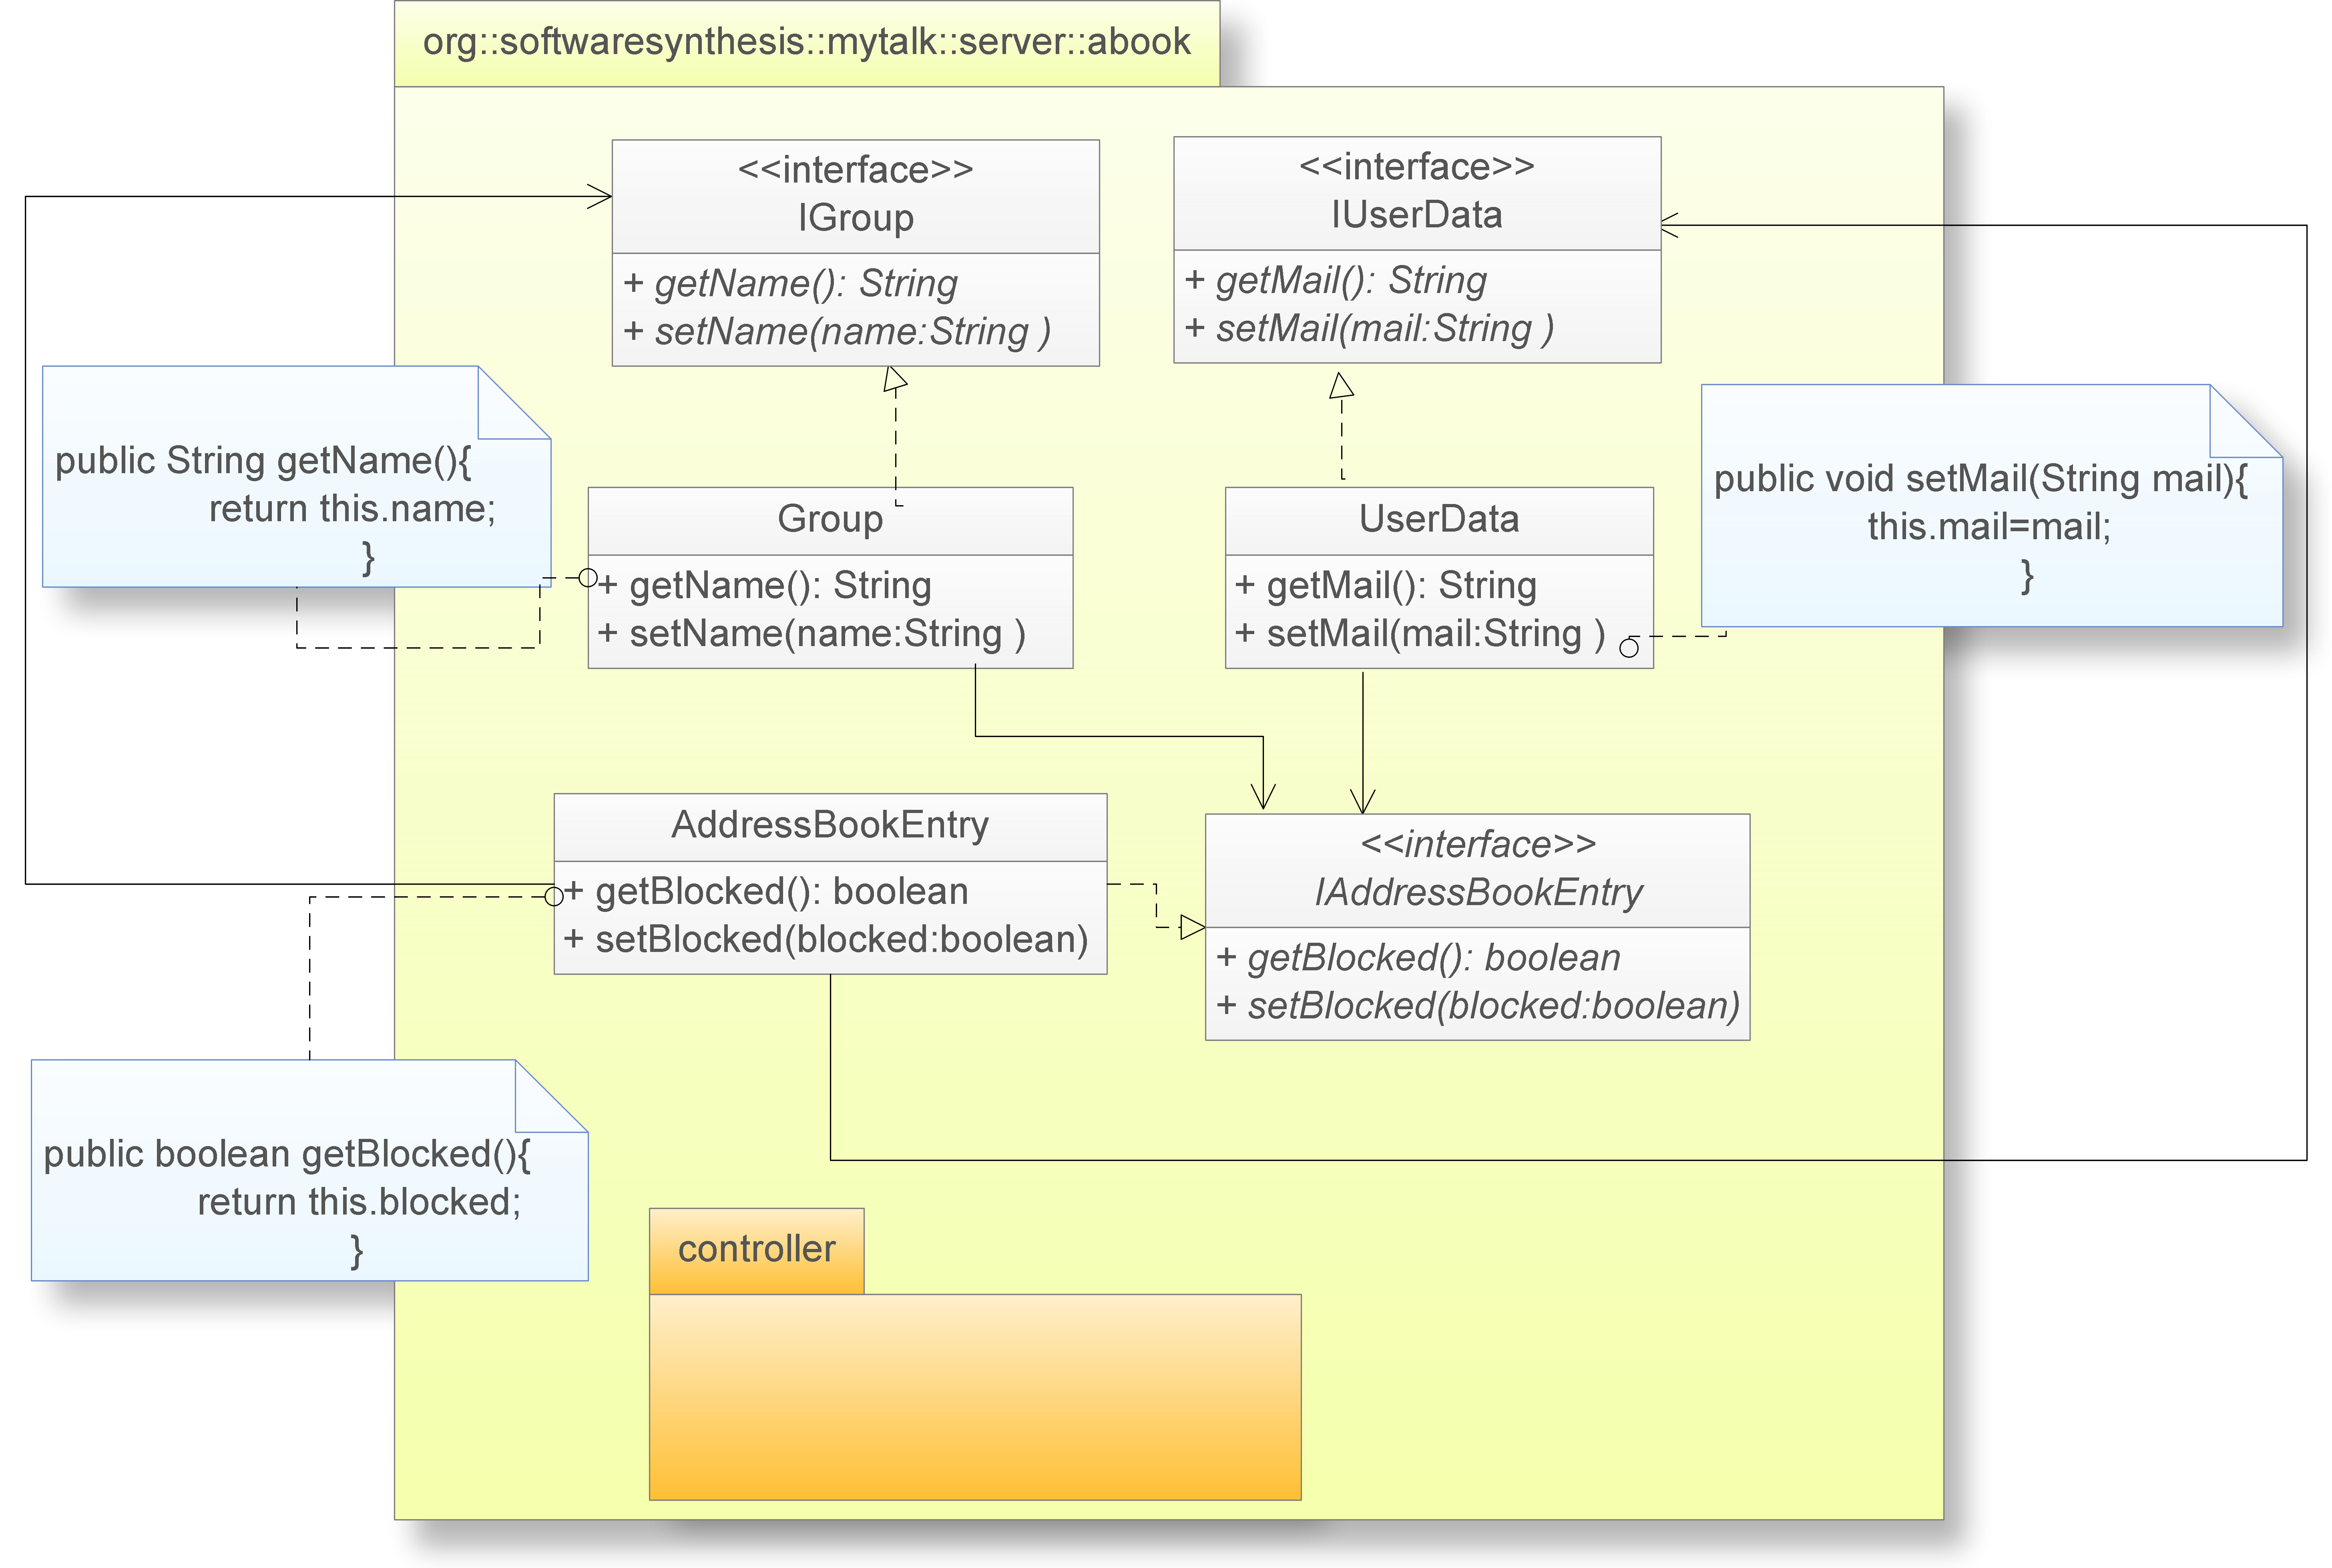
\includegraphics[width=\textwidth]{DDPAbook}
\caption{Diagramma package server.abook}
\end{figure}

\classsection{IUserData}

\subsubsection*{Funzione}
Interfaccia rappresentante il comportamento di un generico utente del sistema. L'interfaccia dovrà definire dei metodi di tipo \textit{get} e \textit{set} per i dati d'interesse.

\subsubsection*{Relazioni d'uso}

\begin{itemize}
	\item \classname{AddressBookEntry}: l'interfaccia definisce dei metodi per la manipolazione di dati \classname{AddressBookEntry}.
\end{itemize}

\subsubsection*{Classi estese ed interfacce implementate}
\begin{itemize}
	\item \texttt{org.softwaresynthesis.mytalk.server.IMyTalkObject}: interfaccia da estendere. Ogni oggetto che implementerà l'interfaccia \classname{IUserData} dovrà essere in grado di convertire il proprio contenuto informativo in formato JSON.
\end{itemize}


\subsubsection*{Metodi}
\begin{description}
	\item{\method{+ getId(): Long}}\\
	Restituisce l'identificatore univoco di uno \classname{IUserData}.
	\item{\method{+ getEmail(): String}}\\
	Restituisce l'indirizzo e-mail con cui uno \classname{IUserData} si è registrato nel sistema \caName.
	\item{\method{+ setEmail(mail: String): void}}\\ 
	Imposta l'indirizzo e-mail con cui si registra nel sistema \caName uno \classname{IUserData}.
	\item{\method{+ getPassword(): String}}\\
	Restituisce la \textit{password} di accesso al sistema \caName di uno \classname{IUserData}.
	\item{\method{+ setPassword(password: String): void}}\\
	Imposta la \textit{password} di accesso al sistema di uno \classname{IUserData}.
	\item{\method{+ getQuestion(): String}}\\
	Restituisce la domanda segreta, scelta da uno \classname{IUserData}, per il recupero della \textit{password} smarrita di accesso al sistema \caName.
	\item{\method{+ setQuestion(question: String): void}}\\
	Imposta la domanda segreta, scelta da uno \classname{IUserData}, per il recupero della \textit{password} smarrita di accesso al sistema \caName.
	\item{\method{+ getAnswer(): String}}\\
	Restituisce la risposta alla domanda per il recupero della \textit{password} smarrita di accesso al sistema \caName.
	\item{\method{+ setAnswer(answer: String): void}}\\
	Imposta la risposta alla domanda segreta per il recupero della \textit{password} di accesso al sistema \caName.
	\item{\method{+ getName(): String}}\\
	Restituisce il nome di uno \classname{IUserData}.
	\item{\method{+ setName(name: String): void}}\\
	Imposta il nome di uno \classname{IUserData}.
	\item{\method{+ getSurname(): String}}\\
	Restituisce il cognome di uno \classname{IUserData}.
	\item{\method{+ setSurname(surname: String): void}}\\
	Imposta il cognome di uno \classname{IUserData}.
	\item{\method{+ getPicturePath(): String}}\\
	Restituisce una stringa con il percorso dell'immagine del profilo di uno \classname{IUserData}.
	\item{\method{+ setPicturePath(path: String): void}}\\
	Imposta il percorso dell'immagine profilo di uno \classname{IUserData}.
	\item{\method{+ getAddressBook(): Set<AddressBookEntry>}}\\
	Metodo che ritorna il la rubrica dell'utente sotto forma d'insieme di \classname{AddressBookEntry}.
	\item{\method{+ addAddressBookEntry(entry: AddressBookEntry): void}}\\
	Metodo usato per aggiungere una nuova \classname{AddressBookEntry} all'insieme di \inglese{entry} che costituisce la rubrica utente.
\end{description}

\classsection{IGroup}

\subsubsection*{Funzione}
Interfaccia rappresentante un gruppo di una rubrica utente del sistema \caName.

\subsubsection*{Relazioni d'uso}

Nessuna relazione evidenziata.

\subsubsection*{Classi estese ed interfacce implementate}
\begin{itemize}
		\item \texttt{org.softwaresynthesis.mytalk.server.IMyTalkObject}: interfaccia da estendere. Ogni oggetto che implementerà l'interfaccia \classname{IGroup} dovrà essere in grado di convertire il proprio contenuto informativo in formato JSON
\end{itemize}

\subsubsection*{Metodi}
\begin{description}
	\item{\method{+ getId(): Long}}\\
	Restituisce l'identificativo univoco di uno gruppo di una rubrica utente.
	\item{\method{+ getName(): String}}\\
	Restituisce il nome di un gruppo di una rubrica utente.
	\item{\method{+ setName(name: String): void}}\\
	Imposta il nome di un gruppo di una rubrica utente.
\end{description}

\classsection{IAddressBookEntry}

\subsubsection*{Funzione}
Interfaccia rappresentante una \textit{entry} di una rubrica utente del sistema mytalk.

\subsubsection*{Relazioni d'uso}
\begin{itemize}
	\item \classname{IUserData}: l'interfaccia \classname{IAddressBookEntry} definisce più metodi che restituiscono oggetti aventi tipo di ritorno \classname{IUserData}, essi sono i metodi \inglese{get} per ottenere il ``proprietario'' della rubrica e l'utente registrato nella rubrica. Analogamente \classname{IUserData} viene usato come parametro d'ingresso per i metodi \inglese{set} collegati ai metodi già citati.
\end{itemize}

\subsubsection*{Classi estese ed interfacce implementate}
\begin{itemize}
		\item \texttt{org.softwaresynthesis.mytalk.server.IMyTalkObject}: interfaccia da estendere. Ogni oggetto che implementerà l'interfaccia \classname{IAddressBookEntry} dovrà essere in grado di convertire il proprio contenuto informativo in formato JSON.
\end{itemize}

\subsubsection*{Metodi}
\begin{description}
	\item{\method{+ getId(): Long}}\\
	Restituisce l'identificativo univoco di una \inglese{entry} di una rubrica utente del sistema \caName.
	\item{\method{+ getEntry(): IUserData}}\\
	Restituisce un istanza di un oggetto avente tipo \classname{IUserData} rappresentante un contatto della rubrica.
	\item{\method{+ setEntry(contact: IUserData): void}}\\
	Imposta l'utente \classname{IUserData} (passato come parametro d'ingresso) come contatto della rubrica.
	\item{\method{+ getGroup(): IGroup}}\\
	Restituisce il gruppo a cui appartiene lo \classname{IUserData} registrato nella rubrica.
	\item{\method{+ setGroup(group: IGroup): void}}\\
	Imposta il gruppo di appartenenza dello \classname{IUserData} registrato nella rubrica.
	\item{\method{+ getOwner(): IUserData}}\\
	Restituisce lo \classname{IUserData} possessore dell'\inglese{entry} corrente della rubrica
	\item{\method{+ setOwner(owner: IUserData ): void}}\\
	Imposta l'utente \classname{IUserData} possessore della \inglese{entry} della rubrica.
\end{description}

\classsection{UserData}

\subsubsection*{Funzione}
Implementazione dell'interfaccia \classname{IUserData}. Un istanza della classe dovrà rappresentare un generico utente del sistema definendone gli attributi e i metodi per impostare ed ottenere il contenuto dei medesimi.

\subsubsection*{Relazioni d'uso}

Nessuna relazione evidenziata

\subsubsection*{Classi estese ed interfacce implementate}
\begin{itemize}
		\item{IUserData}: interfaccia da implementare.
\end{itemize}

\subsubsection*{Attributi}

\begin{itemize}
	\item{\memberdata{-- id: long}}
	Attributo che definisce il codice identificativo con il quale l'utente è registrato nel database del sistema.
	\item{\memberdata{-- mail: String}}
	Attributo che definisce l'indirizzo e-mail con il quale l'utente si è registrato nel sistema.
	\item{\memberdata{-- password: String}}
	Attributo che definisce la \inglese{password} per il \inglese{login} dell'utente nel sistema.
	\item{\memberdata{-- question: String}}
	Attributo che definisce la domanda segreta usata dall'utente in caso di smarrimento della \textit{password}.
	\item{\memberdata{-- answer: String}}
	Attributo che definisce la risposta alla domanda segreta definita nell'attributo \memberdata{question}.
	\item{\memberdata{-- name: String}}
	Attributo che definisce il nome dell'utente.
	\item{\memberdata{-- surname: String}}
	Attributo che definisce il cognome dell'utente.
	\item{\memberdata{-- path: String}}
	Attributo che definisce il percorso (sul server) in cui è memorizzata l'immagine del profilo dell'utente.
	\item{\memberdata{-- addressBook: Set<AddressBookEntry>}}
	Attributo che definisce l'insieme di \classname{AddressBookEntry} che costituiscono la rubrica dell'utente.
	
\end{itemize}

\subsubsection*{Metodi}

\begin{description}
	\item{\method{+ getId(): Long}}\\
	Restituisce l'identificatore univoco di un utente, ritornando l'attributo \memberdata{id}.
	\item{\method{\# setId(id: long): void}}\\
	Imposta l'indirizzo \textit{id} con cui l'utente si registra nel sistema \caName. Il metodo sovrascrive il contenuto dell'attributo \memberdata{id} con il valore tipo \texttt{long} ricevuto come parametro d'ingresso ritornando l'attributo \memberdata{id}.
	\item{\method{+ getEmail(): String}}\\
	Restituisce l'indirizzo e-mail con cui uno l'utente si è registrato nel sistema \caName, ritornando il contenuto dell'attributo \memberdata{mail}.
	\item{\method{+ setEmail(mail: String): void}}\\ 
	Imposta l'indirizzo e-mail con cui l'utente si registra nel sistema \caName. Il metodo non fa altro che sovrascrivere il contenuto dell'attributo \memberdata{mail} con il valore tipo \texttt{String} ricevuto come parametro d'ingresso.
	\item{\method{+ getPassword(): String}}\\
	Restituisce la \inglese{password} dell'utente, ritornando il valore contenuto nell'attributo \memberdata{password}.
	\item{\method{+ setPassword(password: String): void}}\\
	Imposta la \inglese{password} di accesso al sistema, sovrascrivendo il contenuto dell'attributo \memberdata{password} con il valore di tipo \texttt{String} ricevuto come parametro d'ingresso.
	\item{\method{+ getQuestion(): String}}\\
	Restituisce la domanda segreta, scelta dall'utente, per il recupero della \inglese{password} di accesso al sistema \caName. Nello specifico il metodo restituisce il contenuto dell'attributo \memberdata{question}.
	\item{\method{+ setQuestion(question: String): void}}\\
	Imposta la domanda segreta da inserire in caso di smarrimento della \inglese{password}. Il metodo sovrascrive il contenuto dell'attributo \memberdata{question} con il valore tipo \texttt{String} ricevuto come parametro d'ingresso
	\item{\method{+ getAnswer(): String}}\\
	Restituisce la risposta alla domanda per il recupero della \inglese{password} (smarrita) di accesso al sistema \caName. Il metodo ritorna il contenuto dell'attributo \memberdata{answer}.
	\item{\method{+ setAnswer(answer: String): void}}\\
	Imposta la risposta alla domanda segreta per il recupero della \inglese{password}. Il metodo sovrascrive il contenuto dell'attributo \memberdata{answer} con il valore tipo \texttt{String} passato come parametro d'ingresso.
	\item{\method{+ getName(): String}}\\
	Restituisce il nome dell'utente ritornando il contenuto dell'attributo \memberdata{name}.
	\item{\method{+ setName(name: String): void}}\\
	Imposta il nome dell'utente sovrascrivendo il contenuto dell'attributo \memberdata{name} con il valore tipo \texttt{String} passato al metodo come parametro d'ingresso.
	\item{\method{+ getSurname(): String}}\\
	Restituisce il cognome dell'utente restituendo il contenuto dell'attributo \memberdata{surname}.
	\item{\method{+ setSurname(surname: String): void}}\\
	Imposta il cognome dell'utente sovrascrivendo il contenuto dell'attributo \memberdata{surnamename} con il valore tipo \texttt{String} passato al metodo come parametro d'ingresso.
	\item{\method{+ getPicturePath(): String}}\\
	Restituisce una stringa con il percorso dell'immagine del profilo dell'utente, restituendo il contenuto dell'attributo \memberdata{path}.
	\item{\method{+ setPicturePath(path: String): void}}\\
	Imposta il percorso dell'immagine profilo di un utente, sovrascrivendo il contenuto dell'attributo \memberdata{path} con il valore tipo \texttt{String} passato al metodo come parametro d'ingresso.
	\item{\method{+ getState(): State}}\\
	Restituisce lo stato in cui si trova l'utente, ritornando il contenuto dell'attributo \memberdata{state}.
	\item{\method{+ setState(state: State): void}}\\
	Imposta lo stato in cui si trova l'utente, sovrascrivendo il contenuto dell'attributo \memberdata{state} con il valore ricevuto come parametro d'ingresso.
	\item{\method{+ getAddressBook(): Set<AddressBookEntry>}}\\
	Metodo che ritorna il contenuto di \memberdata{addressBook}.
	\item{\method{+ addAddressBookEntry(entry: AddressBookEntry): void}}\\
	Metodo usato per aggiungere ad \memberdata{addressBook} una nuova \classname{AddressBookEntry} passata come parametro d'ingresso.
	\item{\method{+ toJson(): String}}\\
	Metodo usato per ritornare il contenuto di un istanza di \classname{UserData} sotto forma di stringa formattata in JSON. La stringa ritornata deve corrispondere al seguente formato:\\\\
	\verb|{name:"mio_nome",surname:"mio_cognome",email:"mia_mail"|\\\verb|,picturePath:"mia_immagine",id:"mio_id"}|\\
	
	dove i valori tra virgolette rappresentano il contenuto dei rispettivi campi dati contenuti nella classe.
\end{description}

\classsection{Group}

\subsubsection*{Funzione}
Implementazione dell'interfaccia \classname{IGroup}.

\subsubsection*{Relazioni d'uso}

Nessuna relazione evidenziata.

\subsubsection*{Classi estese ed interfacce implementate}
\begin{itemize}
	\item \classname{IGroup}: interfaccia d'implementazione.
\end{itemize}


\subsubsection*{Attributi}

\begin{itemize}
	\item{\memberdata{-- id: long}}
	Attributo del codice identificativo del gruppo.
	\item{\memberdata{-- name: String}}:
	Attributo del nome del gruppo.
\end{itemize}

\subsubsection*{Metodi}

\begin{description}
	\item{\method{+ getId(): Long}}\\
	Restituisce l'identificativo univoco di uno gruppo di una rubrica utente.
	\item{\method{+ getName(): String}}\\
	Restituisce il nome di un gruppo di una rubrica utente.
	\item{\method{+ setName(name: String): void}}\\
	Imposta il nome di un gruppo di una rubrica utente.
	\item{\method{+ toJson(): String}}\\
	Metodo usato per ritornare il contenuto di un istanza di \classname{Group} sotto forma di stringa formattata in JSON. La stringa ritornata deve corrispondere al seguente formato:\\\\
	\verb|{id:"mio_id",name:"mio_nome"}|\\
	
	dove i valori tra virgolette rappresentano il contenuto dei rispettivi campi dati contenuti nella classe.
\end{description}

\classsection{AddressBookEntry}

\subsubsection*{Funzione}
Implementazione dell'interfaccia IAddressBookEntry.

\subsubsection*{Relazioni d'uso}

\begin{itemize}
	\item \classname{IUserData}: usata per definire gli attributi destinati a identificare il possessore dell'istanza di \classname{AddressBookEntry} e il relativo contatto in essa registrato.
\end{itemize}

\subsubsection*{Classi estese ed interfacce implementate}
\begin{itemize}
	\item \classname{IAddressBookEntry}: interfaccia d'implementazione della classe.
\end{itemize}

\subsubsection*{Attributi}

\begin{itemize}
	\item{\memberdata{-- id: long}}
	Attributo del codice identificativo della classe.
	\item{\memberdata{-- group: IGroup}}
	Attributo destinato a identificare il gruppo a cui appartiene il contatto \classname{IUserName} registrato nella classe. Si ricorda che il contatto può anche non appartenere ad alcun gruppo.
	\item{\memberdata{-- contact: IUserData}}
	Attributo destinato ad identificare il contatto registrato nell'istanza di \classname{AddressBookEntry}.
	\item{\memberdata{-- owner: IUserData}}:
	Attributo destinato ad identificare il possessore dell'istanza di \classname{AddressBookEntry}.
	\item{\memberdata{-- blocked: boolean}}
	Attributo booleano necessario per bloccare il contatto, avviene impostando l'attributo a \textit{true}.
\end{itemize}


\subsubsection*{Metodi}

\begin{description}
	\item{\method{+ getId(): Long}}\\
	Restituisce l'identificativo univoco della \inglese{entry} di una rubrica utente del sistema \caName, nello specifico il contenuto dell'attributo \memberdata{id}.
	\item{\method{+ getEntry(): IUserData}}\\
	Restituisce il contenuto dell'attributo \memberdata{contact}.
	\item{\method{+ setEntry(contact: IUserData): void}}\\
	Imposta l'utente \classname{IUserData} (passato come parametro d'ingresso) come contatto della rubrica, nello specifico il contenuto dell'attributo \memberdata{contact}.
	\item{\method{+ getGroup(): IGroup}}\\
	Restituisce il gruppo a cui appartiene lo \classname{IUserData} registrato nella rubrica, nello specifico il contenuto dell'attributo \memberdata{group}.
	\item{\method{+ setGroup(group: IGroup): void}}\\
	Imposta il gruppo di appartenenza dello \classname{IUserData} registrato nella rubrica, nello specifico il contenuto dell'attributo \memberdata{group}.
	\item{\method{+ getOwner(): IUserData}}\\
	Restituisce lo \classname{IUserData} possesore di questa \inglese{entry} della rubrica, nello specifico il contenuto dell'attributo \memberdata{owner}.
	\item{\method{+ setOwner(owner: IUserData ): void}}\\
	Imposta l'utente \classname{IUserData} possessore della \textit{entry} della rubrica, nello specifico il contenuto dell'attributo \memberdata{owner}.
	\item{\method{+ toJson(): String}}\\
	Metodo usato per ritornare il contenuto di un istanza di \classname{AddressBookEntry} sotto forma di stringa formattata in JSON. La stringa ritornata deve corrispondere al seguente formato:\\\\
	\verb|{id:"mio_id",contact:"mio_contatto",group:"mia_gruppo",blocked:"bloccato"}|\\
	
	dove i valori tra virgolette rappresentano il contenuto dei rispettivi campi dati contenuti nella classe.

\end{description}

\subsection{Package \texttt{org.softwaresynthesis.mytalk.server.abook.controller}}\label{sec:call}

\begin{center}
\begin{figure}[H]
  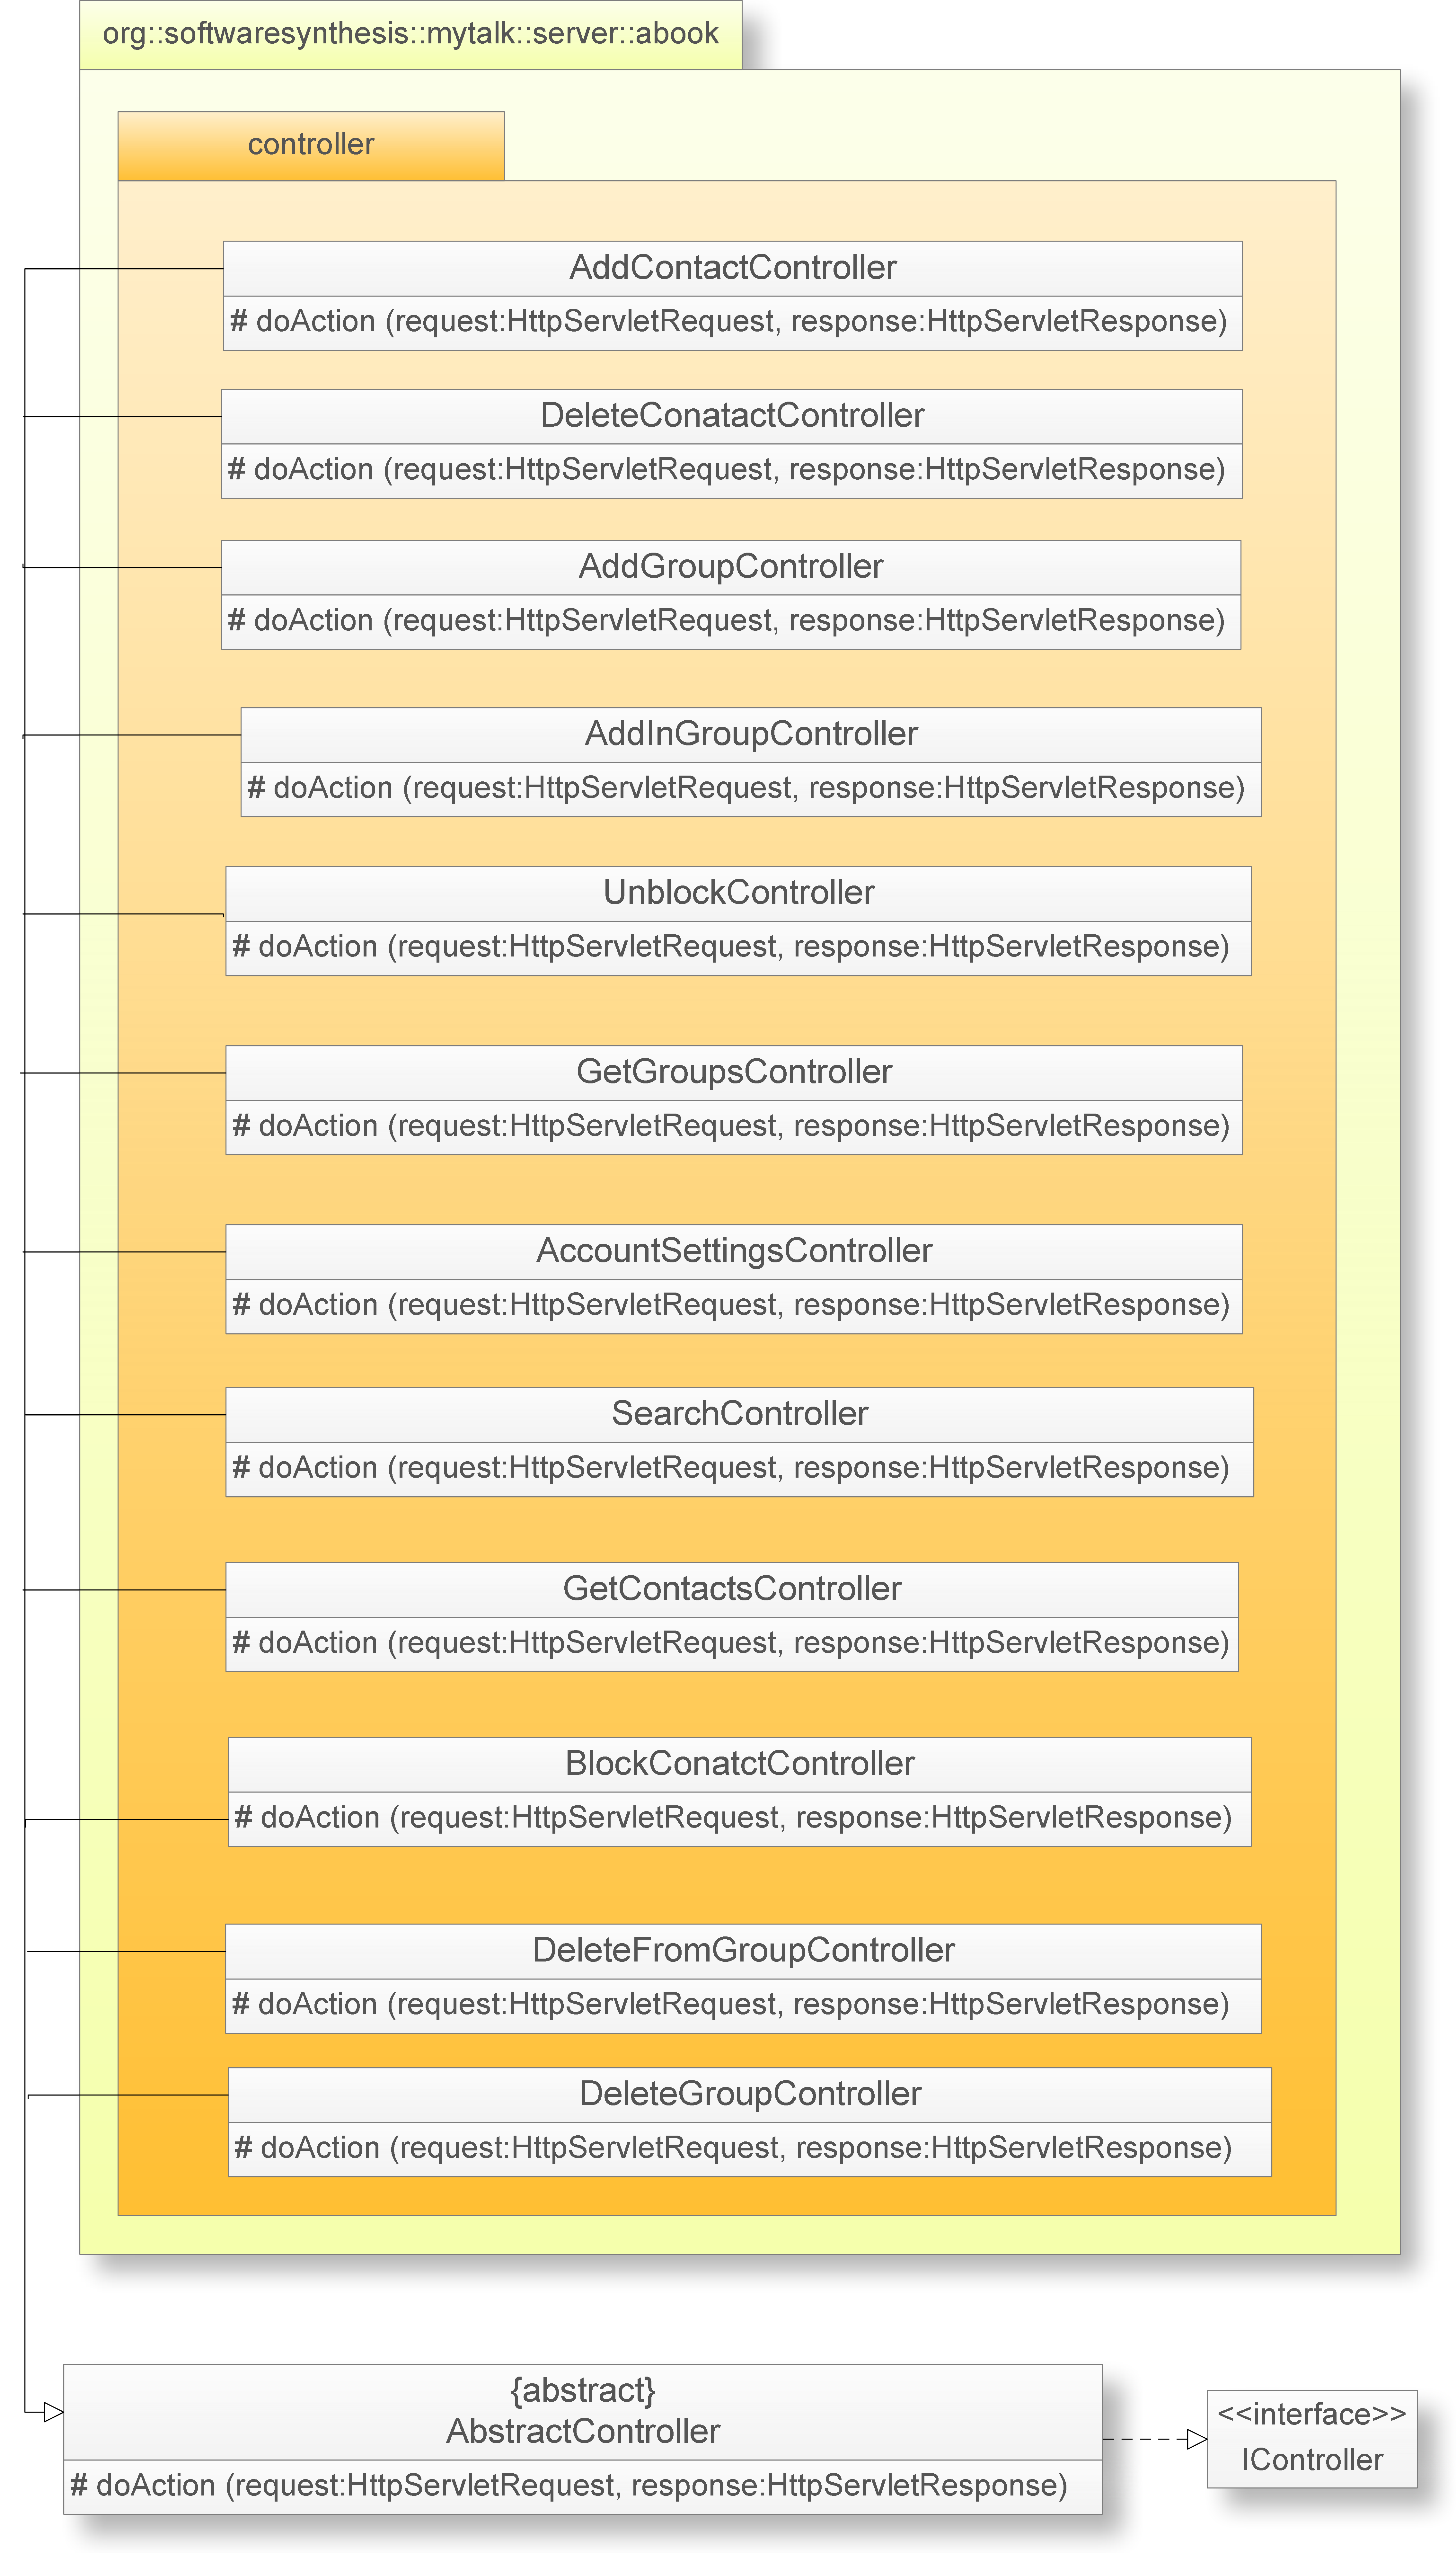
\includegraphics[width=.5\textwidth]{DDPAbookController}
\caption{Diagramma package server.abook.controller}
\end{figure}
\end{center}

%TODO da verificare

\classsection{AddContactController}

\subsubsection*{Funzione}
\textit{Controller} che ha il compito di aggiungere alla rubrica un nuovo contatto.

\subsubsection*{Relazioni d'uso}

\begin{itemize}
	\item \texttt{java.io.IOException}: eccezione richiamabile dal metodo \method{doAction()}.
	\item \texttt{java.io.PrintWriter}: classe istanziata all'interno del metodo \method{doAction()}. Usata per scrivere l'output del \inglese{controller}.
	\item \texttt{javax.servlet.ServletException}: eccezione sollevabile dai metodi \method{doAction()}.
	\item \texttt{javax.servlet.http.HttpServletRequest}: classe usata per interagire con le richieste AJAX inoltrate dal client.
	\item \texttt{javax.servlet.http.HttpServletResponse}: classe usata per interagire con le richieste AJAX inoltrate dal client.
	\item \classname{org.softwaresynthesis.mytalk.server.dao.DataPersistenceManager}: classe usata per comunicare tramite Hibernate con la tabella UserData della base di dati.
\end{itemize}

\subsubsection*{Classi estese ed interfacce implementate}
\begin{itemize}
	\item \texttt{server.AbstractController}: classe estesa.
\end{itemize}

\subsubsection*{Attributi}

Nessun attributo evidenziato

\subsubsection*{Metodi}
\begin{description}
	\item{\method{\# doAction(request HttpServletRequest, response HttpServletResponse): void}}\\	
	Metodo usato per eseguire la richiesta di aggiungere un nuovo contatto all'interno della rubrica. Il flusso principale inizia  con la creazione di un oggetto \classname{dao.DataPersistanceManager} avente nome \texttt{userDAO}. Quindi viene aperto un blocco try catch in cui vengono eseguite le seguenti istruzioni:
	\begin{itemize}
		\item salvare in un attributo di tipo \texttt{long}, \texttt{contactID}, l'\texttt{id} dell'utente. Tale id dovrà essere ottenuto con una chiamata:\\
		\verb|request.getParameter("contactId")|;\\
		
		\item si crea un istanza di tipo \classname{IUserData} che conterrà l'utente che dovrà essere registrato nella rubrica del proprietario. L'oggetto dovrà essere istanziato in seguito ad una chiamata:\\
		\verb|userDAO.getUseData(contactId)|;
		
		\item si crea un istanza di tipo \classname{IUserData} che conterrà l'utente che ha richiesto l'operazione. Tale utente sarà aggiunto alla rubrica del contatto precedentemente aggiunto alla propria.
	\end{itemize}
	
	Quindi se il contatto (che dovrò andare a registrare) è stato correttamente istanziato (\texttt{contatto} != \texttt{null}) allora il flusso principale procede creando e impostando un istanza di \classname{AddressBookEntry}. Il metodo termina ``scrivendo'' \texttt{true} all'interno di un istanza di \texttt{PrintWriter} creata a partire da \texttt{response.getWriter()} ed eseguendo il metodo \method{addAddressBookEntry()} (passando l'\textit{entry} creata in precedenza) a partire dall'istanza che rappresenta l'utente richiedente.
	
	Se invece si è osservato che l'oggetto contenente il contatto da aggiungere, ha valore uguale a \texttt{null}, allora il metodo termina scrivendo \texttt{false} all'intero della dello stesso \texttt{PrintWriter} già citato.
\end{description}

%TODO da verificare

\classsection{DeleteContactsController}

\subsubsection*{Funzione}
\inglese{Controller} richiamata dal \textit{front controller} per eseguire l'eliminazione di un contatto presente nella propria rubrica.

\subsubsection*{Relazioni d'uso}

\begin{itemize}
		\item \texttt{java.io.IOException}: eccezione richiamabile dal metodo \method{doAction()}.
	\item \texttt{java.io.PrintWriter}: classe istanziata all'interno del metodo \method{doAction()}. Usata per scrivere l'output del \inglese{controller}.
	\item \texttt{javax.servlet.ServletException}: eccezione sollevabile dai metodi \method{doAction()}.
	\item \texttt{javax.servlet.http.HttpServletRequest}: classe usata per interagire con le richieste AJAX inoltrate dal client.
	\item \texttt{javax.servlet.http.HttpServletResponse}: classe usata per interagire con le richieste AJAX inoltrate dal client. 
	\item \classname{org.softwaresynthesis.mytalk.server.dao.DataPersistanceManager}: classe usata per comunicare tramite Hibernate con la tabella UserData della base di dati.
\end{itemize}

\subsubsection*{Classi estese ed interfacce implementate}
\begin{itemize}
	\item \texttt{server.AbstractController}: classe estesa.
\end{itemize}

\subsubsection*{Attributi}

Nessun attributo evidenziato

\subsubsection*{Metodi}
\begin{description}
	\item{\method{\# doAction(request HttpServletRequest, response HttpServletResponse): void}}\\	
	Metodo usato per eseguire la richiesta di eliminazione di un contatto presente all'interno della rubrica. Tale metodo deve creare un istanza di \texttt{AddressBookEntry} con i dati relativi alla \textit{entry} da eliminare, quindi richiamerà il metodo \method{removeAddressBookEntry()} a partire dalle due istanze di \texttt{IUserData} (quella che rappresenta l'utente richiedete e quella che rappresenta l'utente da eliminare) passando come parametro l'\textit{entry} definita in precedenza. Più nello specifico Il flusso principale inizia  con la creazione di un oggetto \classname{dao.DataPersistanceManager} avente nome \texttt{userDAO}. Quindi viene aperto un blocco try catch in cui vengono eseguite le seguenti istruzioni::
	\begin{itemize}
		\item salvare in attributo di tipo \texttt{long}, \texttt{contactID}, l'\texttt{id} dell'utente. Tale id dovrà essere ottenuto con una chiamata:\\
		\verb|request.getParameter("contactId")|;\\
		
		\item si crea un istanza di tipo \classname{IUserData} che conterrà ``l'utente'' che dovrà essere eliminato dalla rubrica del chiamante. L'oggetto dovrà essere istanziato in seguito ad una chiamata:\\
		\verb|userDAO.getUserData(contactId)|;
	\end{itemize}
	Quindi se il contatto (che dovrò andare a cancellare dalla lista) è stato correttamente istanziato (\texttt{contatto != null}) allora il flusso principale procede creando e impostando un istanza di \classname{AddressBookEntry}. Quindi a partire dall'oggetto che rappresenta l'utente richiedente, viene richiamato il metodo \method{removeAddressBookEntry()}. Il metodo termina ``scrivendo'' \texttt{true} all'interno di un istanza di \texttt{PrintWriter} creata a partire da \texttt{response.getWriter()}.
	
	Se invece si è osservato che l'oggetto contenente il contatto da rimuovere, ha valore uguale a \texttt{null}, allora il metodo termina impostando \texttt{false} all'intero della dello stesso \texttt{PrintWriter} già citato.
\end{description}

%TODO da verificare

\classsection{AddGroupController}

\subsubsection*{Funzione}
\inglese{Controller} richiamata dal \textit{front controller} per creare un nuovo gruppo nella propria rubrica.

\subsubsection*{Relazioni d'uso}

\begin{itemize}
	\item \texttt{java.io.IOException}: eccezione richiamabile dal metodo \method{doAction()}.
	\item \texttt{java.io.PrintWriter}: classe istanziata all'interno del metodo \method{doAction()}. Usata per scrivere l'output del \inglese{controller}.
	\item \texttt{javax.servlet.ServletException}: eccezione sollevabile dai metodi \method{doAction()}.
	\item \texttt{javax.servlet.http.HttpServletRequest}: classe usata per interagire con le richieste AJAX inoltrate dal client.
	\item \texttt{javax.servlet.http.HttpServletResponse}: classe usata per interagire con le richieste AJAX inoltrate dal client.
	\item \classname{org.softwaresynthesis.mytalk.server.dao.DataPersistanceManager}: classe usata per comunicare tramite Hibernate con la tabella \texttt{UserData} della base di dati.
\end{itemize}

\subsubsection*{Classi estese ed interfacce implementate}
\begin{itemize}
	\item \texttt{server.AbstractController}: classe estesa.
\end{itemize}

\subsubsection*{Attributi}

Nessun attributo evidenziato

\subsubsection*{Metodi}
\begin{description}
	\item{\method{\# doAction(request HttpServletRequest, response HttpServletResponse): void}}\\	
	Metodo usato per eseguire la richiesta di creazione di un gruppo. Nell'ordine proposto, devono essere eseguite le seguenti operazioni:
	\begin{itemize}
		\item creazione di un oggetto \classname{dao.DataPersistanceManager} avente nome groupDAO;
		\item creazione di un oggetto \classname{abook.IGroup} avente nome \texttt{group};
		\item creazione di un oggetto \classname{abook.IUserData} avente nome \texttt{user};
		\item creazione di un oggetto \texttt{PrinterWriter} avente nome \texttt{writer};
		\item creazione di due stringhe, \texttt{name} e \texttt{result};
	\end{itemize}
	A questo punto viene creato un blocco \textit{try-catch}. Il blocco \textit{catch} imposta la stringa \texttt{result} a \texttt{false}, il blocco \textit{try} dovrà invece seguire il seguente iter:
	\begin{itemize}
		\item si imposta la variabile user nel seguente modo:
			\begin{itemize}
				\item si procede salvando l'indirizzo mail in una stringa (mail). Tale indirizzo è ottenuto mediante una chiamata a \method{getUserMail()};
				\item si esegue una chiamata a \texttt{userDAO.getUserData(mail)}, il cui valore restituito viene in fine salvato in user;
			\end{itemize}
		\item impostare \texttt{name} con il contenuto del parametro \textit{groupName} presente nell'oggetto \texttt{request};
		\item verificare se \texttt{name} è \texttt{null} o vuoto. Nel caso procedere impostando \texttt{result} a \texttt{false} e uscendo dal blocco \textit{try}.
		\item altrimenti, se \texttt{name} contiene un nome valido si crea un nuovo gruppo (salvandolo nella variabile \texttt{group}), e impostando il nome e l'utente proprietario.
		\item richiamare \method{insert()} a partire dall'istanza \texttt{groupDAO}, passando come parametro \texttt{group} (che ora conterrà in gruppo da inserire nel database). Viene impostato \texttt{result} a \texttt{true},
	il metodo termina scrivendo su \texttt{write} (usando l'omonimo metodo) il valore contenuto in \texttt{result}. 		
	\end{itemize}
	
\end{description}

%TODO da verificare

\classsection{DeleteGroupController}

\subsubsection*{Funzione}
\inglese{Controller} richiamata dal \textit{front controller} per eliminare un gruppo da una rubrica.

\subsubsection*{Relazioni d'uso}

\begin{itemize}
\item \texttt{java.io.IOException}: eccezione richiamabile dal metodo \method{doAction()}.
	\item \texttt{java.io.PrintWriter}: classe istanziata all'interno del metodo \method{doAction()}. Usata per scrivere l'output del controller.
	\item \texttt{javax.servlet.ServletException}: eccezione sollevabile dai metodi \method{doAction()}.
	\item \texttt{javax.servlet.http.HttpServletRequest}: classe usata per interagire con le richieste AJAX inoltrate dal client.
	\item \texttt{javax.servlet.http.HttpServletResponse}: classe usata per interagire con le richieste AJAX inoltrate dal client.
	\item \classname{org.softwaresynthesis.mytalk.server.dao.DataPersistanceManager}: classe usata per comunicare tramite Hibernate con la tabella \texttt{UserData} della base di dati.
\end{itemize}

\subsubsection*{Classi estese ed interfacce implementate}
\begin{itemize}
	\item \texttt{server.AbstractController}: classe estesa.
\end{itemize}

\subsubsection*{Attributi}

Nessun attributo evidenziato

\subsubsection*{Metodi}
\begin{description}
	\item{\method{\# doAction(request HttpServletRequest, response HttpServletResponse): void}}\\	
	Metodo usato per eseguire la richiesta di eliminazione di un gruppo. Nell'ordine proposto, devono essere eseguite le seguenti operazioni:
	\begin{itemize}
		\item creazione di un'istanza di \classname{dao.AddressBookEntryDAO} denominata \texttt{entryDAO};
		\item creazione di un \classname{dao.DataPersistanceManager} denominata \texttt{groupDAO}.
		\item creazione di un'istanza di \classname{abook.IGroup} denominata \texttt{group};
		\item creazione di un istanza di \classname{abook.IAddressBookEntry} denominata \texttt{entry};
		\item creazione di un istanza di \texttt{Iterator<IAddressBookEntry>} denominata \texttt{iterator};
		\item creazione di un istanza di \texttt{PrintWriter} denominata \texttt{writer};
		\item creazione di un \texttt{Set<IAddressBookEntry>} denominato \texttt{entrys};
		\item creazione di una stringa denominata result (utilizzata per registrare il messaggio da stampare sul \texttt{writer});
	\end{itemize} 
	A questo punto deve essere definito un blocco \textit{try-catch}. Dentro il blocco \textit{catch} si  imposta \texttt{result} con il valore \texttt{false}. {try}, il programmatore dovrà definire il seguente iter:
	\begin{itemize}
		\item salvare in \texttt{group} il valore ritornato da una chiamata \method{getByID} a cui passo l'identificativo del gruppo (\texttt{request.getParameter("groupId")}) a partire dall'oggetto \texttt{groupDAO}.
		\item quindi si esegue una verifica sul contenuto di \texttt{group}. Se \texttt{group == null} allora si imposta \texttt{result} a \texttt{false}. Altrimenti si carica in \textit{entry} l'oggetto ritornato da una chiamata \method{getAddressBook()} a partire da \texttt{group}.
		\item a tal punto (sempre dentro al costrutto condizionale \texttt{if(group != null))} si crea un iteratore tramite \texttt{entrys.iterator()} e ciclando con tale iteratore si va a modificare la voce ``gruppo'' di tutti i contati che nella mia rubrica appartengono a tale gruppo (cosi facendo l'eliminazione del gruppo non porterà all'eliminazione dei contatti presenti in tale gruppo).
		\item dunque si esegue la chiamata:
		\verb|groupDAO.delete(group)|\\
		e si imposta \textit{result} a \inglese{true}.
	\end{itemize}
	Il metodo termina scrivendo su \textit{writer} il contenuto di \textit{result}.
	
\end{description}

%TODO da verificare

\classsection{AddInGroupController}

\subsubsection*{Funzione}
\inglese{Controller} richiamato dal \textit{front controller} per inserire un utente nella propria rubrica, all'interno di un gruppo ben determinato.

\subsubsection*{Relazioni d'uso}

\begin{itemize}
	\item \texttt{java.io.IOException}: eccezione richiamabile dal metodo \method{doAction()}.
	\item \texttt{java.io.PrintWriter}: classe istanziata all'interno del metodo \method{doAction()}. Usata per scrivere l'output del \inglese{controller}.
	\item \texttt{javax.servlet.ServletException}: eccezione sollevabile dai metodi \method{doAction()}.
	\item \texttt{javax.servlet.http.HttpServletRequest}: classe usata per interagire con le richieste AJAX inoltrate dal client.
	\item \texttt{javax.servlet.http.HttpServletResponse}: classe usata per interagire con le richieste AJAX inoltrate dal client.
	\item \classname{abook.IAddressBookEntry}:Interfaccia che definisce il comportamento di una generica \inglese{entry} della rubrica utente. La classe che verrà descritta crea istanze di tipo \classname{abook.IAddressBookEntry}.
	\item \classname{abook.IGroup}:
Interfaccia che definisce il comportamento di un gruppo generico. La classe che qui si descrive crea istanze di tipo \classname{abook.IGroup}.
	\item \classname{abook.IUserData}:Interfaccia che definisce il comportamento di un utente generico. La classe che qui si descrive crea istanze di tipo \classname{abook.IUserData}.
	\item \classname{abook.AddressBookEntry}: classe usata per comunicare tramite \textit{Hibernate} con la tabella \texttt{AddressBookEntry} della base di dati.
	\item \classname{dao.DataPersistanceManager}: classe usata per comunicare tramite \textit{Hibernate} con la tabella \texttt{Group} della base di dati.
	\item \classname{dao.DataPersistanceManager}: classe usata per comunicare tramite \textit{Hibernate} con la tabella \texttt{UserData} della base di dati.
\end{itemize}

\subsubsection*{Classi estese ed interfacce implementate}
\begin{itemize}
	\item \texttt{server.AbstractController}: classe estesa.
\end{itemize}

\subsubsection*{Attributi}

Nessun attributo evidenziato

\subsubsection*{Metodi}

\begin{description}
	\item{\method{\# doAction(request HttpServletRequest, response HttpServletResponse): void}}\\	
	Metodo usato per eseguire la richiesta di aggiungere un contatto in un gruppo. Nell'ordine proposto, devono essere eseguite le seguenti operazioni:
	\begin{itemize}
		\item creazione di un istanza di \classname{DataPersistanceManager} denominata groupDAO;
\item si imposta la variabile user nel seguente modo:
			\begin{itemize}
				\item si procede salvando l'indirizzo mail in una stringa (mail). Tale indirizzo è ottenuto mediante una chiamata a \method{getUserMail()};
				\item si esegue una chiamata a \texttt{userDAO.getUserData(mail)}, il cui valore restituito viene in fine salvato in user;
			\end{itemize}
		\item creazione degli oggetti rappresentanti la realtà della rubrica su cui opero: un \texttt{IAddressBookEntry entry}, \texttt{IGroup group}e \texttt{IUserData friend};
		\item creazione di due identificativi di tipo \texttt{long}: \texttt{contactId} e \texttt{groupId}.
		\item creazione di un \texttt{PrintWriter} denominato \textit{writer} e di una stringa \textit{result} usata con lo scopo di memorizzare il contenuto testuale da scrivere sul \texttt{writer} come messaggio di notifica del \inglese{controller};
		\item creazione di un istanza \texttt{DataPersistanceManager} \texttt{userDAO}.
	\end{itemize}
	Dopo questa fase di creazione delle variabili il metodo deve definire un costrutto \textit{try-catch}. All'interno del blocco \textit{catch} dovrà essere predisposta la memorizzazione della parola ``\inglese{false}''. Passando invece alla definizione del blocco \textit{try}, al suo interno si dovranno predisporre le seguenti istruzioni:
	\begin{itemize}
		\item con una procedura analoga alla precedente definisco il contenuto di \texttt{contactID}. Usare \verb|getParameter("contactId")| a partire dall'oggetto \textit{request};
		\item istruzione analoga alla precedente usata per istanziare il contenuto di \texttt{groupId} (nome del parametro da ottenere: \texttt{groupId});
		\item inizializzare \texttt{friend} con una chiamata \method{getById} passando come parametro \texttt{contactId}.
		\item inizializzare \texttt{group} con una chiamata \method{getById} passando come parametro \texttt{groupId}.
		\item il metodo controlla se \texttt{group!=null}. Nel caso il flusso principale prosegue come segue: inizializzazione di \texttt{entry} e modifica dei dati stessi di \texttt{entry} mediante le chiamate a metodo dei vari \texttt{set} che la costituiscono. Nello specifico si intende impostare l'istanza in modo che definisca un contatto in rubrica non bloccato e registrato nel gruppo \textit{group}. Il possessore sarà user e il contatto registrato \texttt{friend}. Quindi viene eseguito l'\inglese{update} tramite una chiamata:\\
		\verb|userDAO.update(user)|
		\texttt{result} viene impostato a \texttt{true} e il programma esce dal costrutto condizionale.
		\item se \texttt{group} non era diverso da \texttt{null} allora si entra nel ramo \textit{else} del costrutto condizionale già citato. \texttt{result} viene impostato a \texttt{false} e il metodo esce dal ramo \textit{else}.
	\end{itemize}
	Il metodo termina scrivendo su \texttt{writer} il contenuto di \texttt{result}.
	
\end{description}

%TODO da verificare

\classsection{DeleteFromGroupController}

\subsubsection*{Funzione}
\inglese{Controller} richiamato dal \textit{front controller} per inserire un utente nella propria rubrica, all'interno di un gruppo ben determinato.

\subsubsection*{Relazioni d'uso}

\begin{itemize}
	\item \texttt{java.io.IOException}: eccezione richiamabile dal metodo \method{doAction()}.
	\item \texttt{java.io.PrintWriter}: classe istanziata all'interno del metodo \method{doAction()}. Usata per scrivere l'output del controller.
	\item \texttt{javax.servlet.ServletException}: eccezione sollevabile dai metodi \method{doAction()}.
	\item \texttt{javax.servlet.http.HttpServletRequest}: classe usata per interagire con le richieste AJAX inoltrate dal client.
	\item \texttt{javax.servlet.http.HttpServletResponse}: classe usata per interagire con le richieste AJAX inoltrate dal client. \classname{abook.IAddressBookEntry}.
	\item \classname{abook.IGroup}:
Interfaccia che definisce il comportamento di un gruppo generico. La classe che verrà descritta crea istanze di tipo \classname{abook.IGroup}.
	\item \classname{abook.IUserData}:Interfaccia che definisce il comportamento di un utente generico. La classe che verrà descritta crea istanze di tipo \classname{abook.IUserData}.
	\item \classname{abook.AddressBookEntry}: classe usata per comunicare tramite Hibernate con la tabella AddressBookEntry della base di dati.
	\item \classname{dao.DataPersistanceManager}: classe usata per comunicare tramite Hibernate con la tabella \texttt{Group} e \texttt{UserData} della base di dati.
\end{itemize}

\subsubsection*{Classi estese ed interfacce implementate}
\begin{itemize}
	\item \texttt{server.AbstractController}: classe estesa.
\end{itemize}

\subsubsection*{Attributi}

Nessun attributo evidenziato


\subsubsection*{Metodi}

\begin{description}
	\item{\method{\# doAction(request HttpServletRequest, response HttpServletResponse): void}}\\	
	Metodo usato per eseguire la richiesta di rimuovere un contatto da un gruppo. Nell'ordine proposto, devono essere eseguite le seguenti operazioni:
	\begin{itemize}
		\item creazione degli oggetti necessari al completamento dell'operazione:
		\begin{itemize}
			\item \classname{DataPersistanceManager} groupDAO;
			\item \classname{IAddressBookEntry} entry;
			\item \classname{IGroup} group;
			\item \classname{IUserData} friend;
			\item \classname{IUserData} user;
			Long contactIdl;
			Long groupId;
			\item \classname{PrintWriter} writer;
			String result;
			\item \classname{DataPersistanceManager} userDAO;
		\end{itemize}
		
		\item quindi il metodo procede definendo un blocco \textit{try-catch}. Nel ramo \textit{catch} si imposta \texttt{result} a \texttt{false}. Passando invece alla definizione del ramo \textit{try}, in esso devono essere definiti i seguenti punti:
		\begin{itemize}
			\item si imposta la variabile user nel seguente modo:
			\begin{itemize}
				\item si procede salvando l'indirizzo mail in una stringa (mail). Tale indirizzo è ottenuto mediante una chiamata a \method{getUserMail()};
				\item si esegue una chiamata a \texttt{userDAO.getUserData(mail)}, il cui valore restituito viene in fine salvato in user;
			\end{itemize}
			
			
			\item impostare \texttt{friend} e \texttt{group} a partire dai relativi tipi di istanze DAO e facendosi restituire i dati presenti nel database tramite una chiamata a metodo \method{getByID} a cui passa i relativi id (\texttt{contactId} e \texttt{groupid});
			\item avvia un costrutto condizionale dotato di ramo \textit{else}, se \texttt{group!=null} allora il metodo procede nel ramo \texttt{if} andando ad impostare \texttt{entry} con i relativi parametri, in modo da ricreare l'istanza \classname{IAddressBookEntry} da rimuovere dal database per mezzo del metodo \method{removeAddressBookEntry()} a cui passa \texttt{entry}. 
			\item altrimenti, se \texttt{group == null} allora entra nel ramo else del costrutto condizionale e procede impostando \texttt{result} a \texttt{false}.
		\end{itemize}
	\end{itemize}
	Il metodo termina scrivendo su \texttt{writer} il contenuto di \texttt{result}.
	
\end{description}

%TODO da verificare

\classsection{BlockContactController}

\subsubsection*{Funzione}
\inglese{Controller} richiamato dal \textit{front controller} per bloccare un contatto presente nella propria rubrica.

\subsubsection*{Relazioni d'uso}

\begin{itemize}
	\item \texttt{java.io.IOException}: eccezione richiamabile dal metodo \method{doAction()}.
	\item \texttt{java.io.PrintWriter}: classe istanziata all'interno del metodo \method{doAction()}. Usata per scrivere l'output del \inglese{controller}.
	\item \texttt{javax.servlet.ServletException}: eccezione sollevabile dai metodi \method{doAction()}.
	\item \texttt{javax.servlet.http.HttpServletRequest}: classe usata per interagire con le richieste AJAX inoltrate dal client.
	\item \texttt{javax.servlet.http.HttpServletResponse}: classe usata per interagire con le richieste AJAX inoltrate dal client.
	\item \classname{abook.IAddressBookEntry}:Interfaccia che definisce il comportamento di una generica \inglese{entry} della rubrica utente. La classe che verrà descritta crea istanze di tipo \classname{abook.IAddressBookEntry}.
	\item \classname{abook.IUserData}:Interfaccia che definisce il comportamento di un utente generico. La classe che verrà descritta crea istanze di tipo \classname{abook.IUserData}.
	\item \classname{dao.DataPersistanceManager}: classe usata per comunicare tramite Hibernate con la tabella \texttt{UserData} della base di dati.
\end{itemize}

\subsubsection*{Classi estese ed interfacce implementate}
\begin{itemize}
	\item \texttt{server.AbstractController}: classe estesa.
\end{itemize}

\subsubsection*{Attributi}

Nessun attributo evidenziato


\subsubsection*{Metodi}

\begin{description}
	\item{\method{\# doAction(request HttpServletRequest, response HttpServletResponse): void}}\\	
	Metodo usato per eseguire la richiesta di bloccare un contatto presente in una rubrica utente. Nell'ordine proposto, devono essere eseguite le seguenti operazioni:
	\begin{itemize}
		\item creazione degli oggetti necessari al completamento dell'operazione:
		\begin{itemize}
			\item \classname{DataPersistanceManager} groupDAO;
			\item \classname{IAddressBookEntry} entry;
			\item \classname{IUserData} friend;
			\item \classname{IUserData} user;
			Long contactIdl;
			\item \texttt{Iterator<IAddressBookEntry>} iterator;
			\item \texttt{Set<IAddressBookEntry>} entrys;
			\item \classname{PrintWriter} writer;
			String result;
			\item \classname{DataPersistanceManager} userDAO;
		\end{itemize}
		
		\item quindi il metodo procede definendo un blocco \textit{try-catch}. Nel ramo \textit{catch} si imposta \texttt{result} a \texttt{false}. Passando invece alla definizione del ramo \textit{try} devono essere definiti i seguenti punti:
		\begin{itemize}
			\item si imposta la variabile user nel seguente modo:
			\begin{itemize}
				\item si procede salvando l'indirizzo mail in una stringa (mail). Tale indirizzo è ottenuto mediante una chiamata a \method{getUserMail()};
				\item si esegue una chiamata a \texttt{userDAO.getUserData(mail)}, il cui valore restituito viene in fine salvato in user;
			\end{itemize}
			\item impostare  \texttt{friend} a partire dal relativo tipo di istanza DAO e facendo restituire i dati presenti nel database tramite una chiamata a metodo \method{getUserData()} a cui passa il parametro \texttt{contactId};
			\item avvia un costrutto condizionale dotato di ramo else. Se \texttt{friend!=null} il metodo procede nel ramo \texttt{if} andando a scaricare l'elenco delle \texttt{entry} a partire da \textit{user}. Quindi utilizzando l'iteratore \texttt{iterator} va a scorrere tale set di \textit{entry} e quando verifica la presenza del contatto \texttt{friend} all'interno, modifica l'\textit{entry} attualmente selezionata richiamando il metodo \method{setBlocked(true)}. Quindi prima di uscire dal costrutto \texttt{if}, viene eseguita un operazione di \textit{update} a partire da user e si memorizza nella variabile \texttt{result} il valore \texttt{true}.
			\item altrimenti, se \texttt{friend == null} allora entra nel ramo else del costrutto condizionale e procede impostando \texttt{result} a \texttt{false}.
		\end{itemize}
	\end{itemize}
	Il metodo termina scrivendo su \texttt{writer} il contenuto di \texttt{result}.
	
\end{description}

%TODO da verificare

\classsection{UnblockContactController}

\subsubsection*{Funzione}
\inglese{Controller} richiamato dal \textit{front controller} per sbloccare un contatto presente nella propria rubrica.

\subsubsection*{Relazioni d'uso}

\begin{itemize}
	\item \texttt{java.io.IOException}: eccezione richiamabile dal metodo \method{doAction()}.
	\item \texttt{java.io.PrintWriter}: classe istanziata all'interno del metodo \method{doAction()}. Usata per scrivere l'output del controller.
	\item \texttt{javax.servlet.ServletException}: eccezione sollevabile dai metodi \method{doAction()}.
	\item \texttt{javax.servlet.http.HttpServletRequest}: classe usata per interagire con le richieste AJAX inoltrate dal client.
	\item \texttt{javax.servlet.http.HttpServletResponse}: classe usata per interagire con le richieste AJAX inoltrate dal client.
	\item \classname{abook.IAddressBookEntry}: interfaccia che definisce il comportamento di una generica \inglese{entry} della rubrica utente. La classe che verrà descritta crea istanze di tipo \classname{abook.IAddressBookEntry}.
	\item \classname{abook.IUserData}: interfaccia che definisce il comportamento di un utente generico. La classe che verrà descritta crea istanze di tipo \classname{abook.IUserData}.
	\item \classname{dao.DataPersistanceManager}: classe usata per comunicare tramite Hibernate con la tabella \texttt{UserData} della base di dati.
\end{itemize}

\subsubsection*{Classi estese ed interfacce implementate}
\begin{itemize}
	\item \texttt{server.AbstractController}: classe estesa.
\end{itemize}

\subsubsection*{Attributi}

Nessun attributo evidenziato

\subsubsection*{Metodi}

\begin{description}
	\item{\method{\# doAction(request HttpServletRequest, response HttpServletResponse): void}}\\	
	Metodo usato per eseguire la richiesta di sbloccare un contatto presente in una rubrica utente. Nell'ordine proposto, devono essere eseguite le seguenti operazioni:
	\begin{itemize}
		\item creazione degli oggetti necessari al completamento dell'operazione:
		\begin{itemize}
			\item \classname{DataPersistanceManager} groupDAO;
			\item \classname{IAddressBookEntry} entry;
			\item \classname{IUserData} friend;
			\item \classname{IUserData} user;
			Long contactIdl;
			\item \texttt{Iterator<IAddressBookEntry>} iterator;
			\item \texttt{Set<IAddressBookEntry>} entrys;
			\item \classname{PrintWriter} writer;
			String result;
			\item \classname{DataPersistanceManager} userDAO;
		\end{itemize}
		
		\item quindi il metodo procede definendo un blocco \textit{try-catch}. Nel ramo \textit{catch} si imposta \texttt{result} a \texttt{false}. Passando invece alla definizione del ramo \textit{try}, in esso devono essere definiti i seguenti punti:
		\begin{itemize}
			\item si imposta la variabile user nel seguente modo:
			\begin{itemize}
				\item si procede salvando l'indirizzo mail in una stringa (mail). Tale indirizzo è ottenuto mediante una chiamata a \method{getUserMail()};
				\item si esegue una chiamata a \texttt{userDAO.getUserData(mail)}, il cui valore restituito viene in fine salvato in user;
			\end{itemize}
			\item impostare\texttt{friend} a partire dal relativo tipo di istanza DAO e facendo restituire i dati presenti nel database tramite una chiamata a metodo \method{getUserData()} a cui passa il parametro \texttt{contactId};
			\item avvia un costrutto condizionale dotato di ramo else. Se \texttt{friend!=null} il metodo procede nel ramo \textit{if} andando a scaricare l'elenco delle \textit{entry} a partire da \texttt{user}. Quindi utilizzando l'iteratore \textit{iterator} va a scorrere tale set di \textit{entry} e quando verifica la presenza del contatto \texttt{friend} all'interno, modifica l'\textit{entry} attualmente selezionata richiamando il metodo \method{setBlocked(false)}. Quindi prima di uscire dal costrutto \texttt{if}, viene eseguita un operazione di \textit{update} a partire da \textit{user} e si memorizza nella variabile \texttt{result} il valore \texttt{true}.
			\item altrimenti, se \texttt{friend == null} allora entra nel ramo else del costrutto condizionale e procede impostando \texttt{result} a \texttt{false}.
		\end{itemize}
	\end{itemize}
	Il metodo termina scrivendo su \texttt{writer} il contenuto di \texttt{result}.
	
\end{description}

%TODO da verificare

\classsection{SearchController}

\subsubsection*{Funzione}
\inglese{Controller} richiamato dal \textit{front controller} per effettuare una ricerca sulla propria rubrica. La ricerca consiste nell'individuare tutti i contatti che contengono nei campi \texttt{name}, \texttt{surname} o \texttt{email} la parola ricercata. Per eseguire questa procedura di ricerca ci si avvale del metodo \method{searchGeneric(nome\_parametro)} della classe \classname{DataPersistanceManager}.

\subsubsection*{Relazioni d'uso}

\begin{itemize}
	\item \texttt{java.io.IOException}: eccezione richiamabile dal metodo \method{doAction()}.
	\item \texttt{java.io.PrintWriter}: classe istanziata all'interno del metodo \method{doAction()}. Usata per scrivere l'output del controller.
	\item \texttt{javax.servlet.ServletException}: eccezione sollevabile dai metodi \method{doAction()}.
	\item \texttt{javax.servlet.http.HttpServletRequest}: classe usata per interagire con le richieste AJAX inoltrate dal client.
	\item \texttt{javax.servlet.http.HttpServletResponse}: classe usata per interagire con le richieste AJAX inoltrate dal client.
	\item \classname{abook.IUserData}:Interfaccia che definisce il comportamento di un utente generico. La classe che verrà descritta crea istanze di tipo \classname{abook.IUserData}.
	\item \classname{dao.DataPersistanceManager}: classe usata per comunicare tramite Hibernate con la tabella \texttt{UserData} della base di dati.
\end{itemize}

\subsubsection*{Classi estese ed interfacce implementate}
\begin{itemize}
	\item \texttt{server.AbstractController}: classe estesa.
\end{itemize}

\subsubsection*{Attributi}

Nessun attributo evidenziato

\subsubsection*{Metodi}

\begin{description}
	\item{\method{\# doAction(request HttpServletRequest, response HttpServletResponse): void}}\\	
	Metodo usato per eseguire una ricerca generica sui contatti presenti nella rubrica del \textit{client}. Nell'ordine proposto, devono essere eseguite le seguenti operazioni:
	\begin{itemize}
		\item creazione degli oggetti necessari al completamento dell'operazione:
		\begin{itemize}
			\item \classname{IUserData} entry;
			\item \texttt{List<IUserData>} users;
			\item \texttt{Iterator<IUserData>} iterator;
			\item \texttt{Set<IAddressBookEntry>} entrys;
			\item \classname{PrintWriter} writer;
			\item String result e String parameter;
			\item \classname{DataPersistanceManager} userDAO;
		\end{itemize}
		
		\item quindi il metodo procede definendo un blocco \textit{try-catch}. Nel ramo \textit{catch} si imposta \texttt{result} a \texttt{false}. Passando invece alla definizione del ramo \textit{try}, in esso devono essere definiti i seguenti punti:
		\begin{itemize}
			\item parameter viene impostato con il valore del parametro da ricercare. Tale operazione è da eseguirsi con l'istruzione:\\
			\verb|request.getParameter("param")|;
			\item quindi il metodo procede effettuando la ricerca del parametro. Tale operazione si svolge sfruttando le specifiche della classe \classname{DataPersistanceManager}. Nello specifico deve essere eseguita l'istruzione:\\
			\verb|users = userDAO.getUserData(parameter)|;
			\item a questo punto si dovrà predisporre un iteratore per scorrere la lista \textit{users};
			\item si imposta \texttt{result} al valore ``{'' e si entra in un ciclo \inglese{while} che potrà terminare solo quando l'iteratore già citato avrà raggiunto l'ultimo elemento ispezionabile;
			\item dentro al ciclo \inglese{while} si procederà con la formattazione della stringa \texttt{result} al fine di restituire al client un formato sul quale possa operare. Nello specifico la stringa \texttt{result} dovrà contenere (per ogni istanza di IUserData presente in \texttt{users}):\\
			
			\verb|\"ID_della_entry":{"name":"NOME_UTENTE",|\\
			\verb|"surname":"COGNOME_UTENTE,"email":EMAIL_UTENTE",|\\
			\verb|"id":"ID_UTENTE","picturePath":"PATH_IMG",|\\
			\verb|"state":"STATO","block":"BLOCCATO/SBLOCCATO"},|\\
			
			Si osservi che in quanto è riportato in precedenza, ciò che è scritto in maiuscolo corrisponde al valore effettivo di quel parametro, quindi per esempio la parola NOME\_UTENTE sarà di fatto sostituita dall'effettivo nome dell'istanza \classname{IUserData} attualmente sotto esame. Per ottenere tali valori ricorrerà ai metodi: \texttt{getName()}, \texttt{getSurname()}, \texttt{getMail()}, \texttt{getId()}, \texttt{getPath()} richiamabili a partire dall'\textit{entry} attualmente sotto esame.
			\item al termine di tale procedura la stringa \texttt{result} è pronta per essere restituita al client, quindi si aggiunge a \texttt{result} il valore ``}'', usato come carattere di terminazione.
		\end{itemize}
	\end{itemize}
	Il metodo termina scrivendo su \texttt{writer} il contenuto di \texttt{result}.
	
\end{description}

%TODO da verificare

\classsection{GetContactsController}

\subsubsection*{Funzione}
\inglese{Controller} richiamato dal \textit{front controller} per scaricare la lista dei contatti presenti nella propria rubrica.

\subsubsection*{Relazioni d'uso}

\begin{itemize}
	\item \texttt{java.io.IOException}: eccezione richiamabile dal metodo \method{doAction()}.
	\item \texttt{java.io.PrintWriter}: classe istanziata all'interno del metodo \method{doAction()}. Usata per scrivere l'output del controllers.
	\item \texttt{javax.servlet.ServletException}: eccezione sollevabile dai metodi \method{doAction()}.
	\item \texttt{javax.servlet.http.HttpServletRequest}: classe usata per interagire con le richieste AJAX inoltrate dal client.
	\item \texttt{javax.servlet.http.HttpServletResponse}: classe usata per interagire con le richieste AJAX inoltrate dal client.
	\item \classname{abook.IAddressBookEntry}:Interfaccia che definisce il comportamento di una \inglese{entry} della rubrica utente.
	\item \classname{abook.IUserData}:Interfaccia che definisce il comportamento di un utente generico. La classe che verrà descritta crea istanze di tipo \classname{abook.IUserData}.
	\item \classname{dao.DataPersistanceManager}: classe usata per comunicare tramite Hibernate con la tabella \texttt{UserData} della base di dati.
\end{itemize}

\subsubsection*{Classi estese ed interfacce implementate}
\begin{itemize}
	\item \texttt{server.AbstractController}: classe estesa.
\end{itemize}

\subsubsection*{Attributi}

Nessun attributo evidenziato

\subsubsection*{Metodi}

\begin{description}
	\item{\method{\# doAction(request HttpServletRequest, response HttpServletResponse): void}}\\	
	Metodo usato per eseguire la richiesta di download della lista dei contatti. Nell'ordine proposto, devono essere eseguite le seguenti operazioni:
	\begin{itemize}
		\item creazione degli oggetti necessari al completamento dell'operazione:
		\begin{itemize}
			\item \classname{IUserData} user;
			\item \classname{IUserData} friend;
			\item \texttt{Iterator<IAddressBookEntry>} iterator;
			\item \texttt{Set<IAddressBookEntry>} entrys;
			\item \classname{PrintWriter} writer;
			\item String result;
			\item \classname{IAddressBookEntry} entry;
		\end{itemize}
		
		\item quindi il metodo procede definendo un blocco \textit{try-catch}. Nel ramo \textit{catch} si imposta \texttt{result} a \texttt{null}. Passando invece alla definizione del ramo \textit{try}, devono essere definiti i seguenti punti:
		\begin{itemize}
			\item si imposta la variabile user nel seguente modo:
			\begin{itemize}
				\item si procede salvando l'indirizzo mail in una stringa (mail). Tale indirizzo è ottenuto mediante una chiamata a \method{getUserMail()};
				\item si esegue una chiamata a \texttt{userDAO.getUserData(mail)}, il cui valore restituito viene in fine salvato in user;
			\end{itemize}
			\item quindi il metodo procede impostando user a partire dalla sessione precedentemente creata. Tale operazione richiede l'uso del metodo \method{getAttribute(``user''};
			\item viene inizializzato l'insieme \texttt{contacts} tramite una chiamata \method{getAddressBook()} richiamata a partire dalla variabile \texttt{user};
			\item a questo punto si dovrà predisporre un iteratore per scorrere l'insieme \textit{contacts};
			\item si imposta \textit{result} al valore ``{'' e si entra in un ciclo \inglese{while} che potrà terminare solo quando l'iteratore già citato avrà raggiunto l'ultimo elemento ispezionabile;
			\item dentro al ciclo \inglese{while}, dopo aver impostato \textit{entry} al valore \texttt{next()} dell'iteratore, viene salvato in \texttt{friend} il contatto ritornato da una chiamata a \textit{entry}.\method{getContact()}. Si procederà  poi con la formattazione della stringa \texttt{result} al fine di restituire al \textit{client} un formato sul quale possa operare. Nello specifico la stringa \texttt{result} dovrà contenere (per ogni istanza di \texttt{IUserData} presente in \texttt{users}):\\
			
			\verb|\"ID_della_entry":{"name":"NOME_UTENTE",|\\
			\verb|"surname":"COGNOME_UTENTE,"email":EMAIL_UTENTE",|\\
			\verb|"id":"ID_UTENTE","picturePath":"PATH_IMG",|\\
			\verb|"state":"STATO","block":"BLOCCATO/SBLOCCATO"},|\\
			
			Si osservi che in quanto è riportato in precedenza, ciò che è scritto in maiuscolo corrisponde al valore effettivo di quel parametro. Quindi per esempio la parola NOME\_UTENTE sarà di fatto sostituita dall'effettivo nome dell'istanza \classname{IUserData} attualmente sotto esame. Per ottenere tali valori si ricorre ai metodi: \texttt{getName()}, \texttt{getSurname()}, \texttt{getMail()}, \texttt{getId()}, \texttt{getPath()} richiamabili a partire da friend.
			\item al termine di tale procedura la stringa \texttt{result} è pronta per essere restituita al client. Quindi si aggiunge a \texttt{result} il valore ``}'', usato come carattere di terminazione.
		\end{itemize}
	\end{itemize}
	Il metodo termina scrivendo su \texttt{writer} il contenuto di \texttt{result}.
	
\end{description}

%TODO da verificare

\classsection{GetGroupsController}

\subsubsection*{Funzione}
\inglese{Controller} richiamato dal \textit{front controller} per scaricare la propria rubrica, provvista di gruppi e contatti in essi presenti.

\subsubsection*{Relazioni d'uso}

\begin{itemize}
	\item \texttt{java.io.IOException}: eccezione richiamabile dal metodo \method{doAction()}.
	\item \texttt{java.io.PrintWriter}: classe istanziata all'interno del metodo \method{doAction()}. Usata per scrivere l'output del \inglese{controller}.
	\item \texttt{javax.servlet.ServletException}: eccezione sollevabile dai metodi \method{doAction()}.
	\item \texttt{javax.servlet.http.HttpServletRequest}: classe usata per interagire con le richieste AJAX inoltrate dal client.
	\item \texttt{javax.servlet.http.HttpServletResponse}: classe usata per interagire con le richieste AJAX inoltrate dal client.
	\item \classname{abook.IAddressBookEntry}:Interfaccia che definisce il comportamento di una \inglese{entry} della rubrica utente.
	\item \classname{abook.IUserData}:Interfaccia che definisce il comportamento di un utente generico. La classe che verrà descritta crea istanze di tipo \classname{abook.IUserData}.
		\item \classname{abook.IGroup}:Interfaccia che definisce il comportamento di un gruppo generico. La classe che verrà descritta crea istanze di tipo \classname{abook.IGroup}.
	\item \classname{dao.DataPersistanceManager}: classe usata per comunicare tramite Hibernate con la tabella \texttt{Group} della base di dati.
\end{itemize}

\subsubsection*{Classi estese ed interfacce implementate}
\begin{itemize}
	\item \texttt{server.AbstractController}: classe estesa.
\end{itemize}

\subsubsection*{Attributi}

Nessun attributo evidenziato

\subsubsection*{Metodi}

\begin{description}
\item{\method{\# doAction(request HttpServletRequest, response HttpServletResponse): void}}\\	
	Metodo usato per eseguire la richiesta di download della lista dei contatti utente). Nell'ordine proposto, devono essere eseguite le seguenti operazioni:
	\begin{itemize}
		\item creazione degli oggetti necessari al completamento dell'operazione:
		\begin{itemize}
			\item \classname{DataPersistanceManager} groupDAO;
			\item \classname{IAddressBookEntry} entry;
			\item \classname{IGroup} group;
			\item \classname{IUserData} user;
			\item \texttt{Iterator<IAddressBookEntry>} entryIter;
			\item \texttt{Iterator<IGroup>} groupIter;
			\item \texttt{Set<IAddressBookEntry>} addentrys;
			\item \classname{PrintWriter} writer;
			\item String result;
		\end{itemize}
		
		\item quindi il metodo procede definendo un blocco \textit{try-catch}. Nel ramo catch si imposta \texttt{result} a \texttt{false}. Passando invece alla definizione del ramo \textit{try}, in esso devono essere definiti i seguenti punti:
		\begin{itemize}
			\item si imposta la variabile user nel seguente modo:
			\begin{itemize}
				\item si procede salvando l'indirizzo mail in una stringa (mail). Tale indirizzo è ottenuto mediante una chiamata a \method{getUserMail()};
				\item si esegue una chiamata a \texttt{userDAO.getUserData(mail)}, il cui valore restituito viene in fine salvato in user;
			\end{itemize}
			\item quindi il metodo procede impostando user a partire dalla sessione precedentemente creata. Tale operazione richiede l'uso del metodo \method{getAttribute(``user'')};
			\item viene inizializzato l'oggetto \texttt{groupDAO};
			\item si inizializza la lista \texttt{groups} dei gruppi. Tale operazione deve essere eseguita mediante l'istruzione:\\
			\verb|groupDAO.getGroup(user.getId())|
			\item il metodo definisce un costrutto condizionale \textit{if-else} basato sulla condizione \texttt{groups != null}. Nel ramo \textit{else} il metodo non fa altro che impostare \texttt{result} a \texttt{false}. Nel ramo \textit{if} saranno definite le seguenti istruzioni:	
			\begin{itemize}
				\item predisporre un iteratore per scorrere l'insieme \texttt{groups} (inizializzazione di groupIter);
				\item si imposta \texttt{result} al valore ``\{'' e si entra in un ciclo \inglese{while} che potrà terminare solo quando l'iteratore già citato avrà raggiunto l'ultimo elemento ispezionabile;
				\item all'interno del ciclo si estrae dall'iteratore il gruppo attualmente in esame e si salva sull'oggetto \texttt{group};
				\item a partire da \texttt{group}, tramite una chiamata \method{getAddressBook()}, si ottiene la lista di \textit{entry} di quel gruppo e la si slava in \texttt{addEntry};
				\item si definisce un nuovo iteratore \texttt{addEntry} \method{iterator()} e lo si memorizza in entryIter;
				\item si ``scrive'' in \texttt{result}, i dati inerenti il gruppo in esame (\texttt{name}, \texttt{id}) e si aggiunge la stringa ``contacts:['';
				\item si entra in un nuovo ciclo \inglese{while} che cicla sulle \textit{entry} dell'iteratore \texttt{entryIter}. All'interno di tale ciclo si estraggono le \textit{entry} che costituiscono i contatti del gruppo in esame e si riporta in \texttt{result} l'id di tali contatti (usare metodo \method{getId()});
				\item all'uscita del ciclo \inglese{while} più interno si concatena al contenuto di \texttt{result} la stringa ``]\}'';
				\item all'uscita del ciclo \inglese{while} più esterno si concatena al contenuto di \texttt{result} la stringa ``\}'';
			\end{itemize}
		\end{itemize}
	\end{itemize}
	Il metodo termina scrivendo su \texttt{writer} il contenuto di \texttt{result}.	
	
\end{description}

\classsection{AccountSettingController}

\subsubsection*{Funzione}
\inglese{Controller} usato per modificare i dati utente. Nello specifico il client potrà operare una modifica ai campi \texttt{nome} e \texttt{cognome}. Lo sviluppatore deve ricordarsi che i dati di autenticazione risiedono nella session con il quale il client sta interagendo con il \textit{front controller}.

\subsubsection*{Relazioni d'uso}

\begin{itemize}
	\item \texttt{java.io.IOException}: eccezione richiamabile dal metodo \method{doAction()}.
	\item \texttt{java.io.PrintWriter}: classe istanziata all'interno del metodo \method{doAction()}. Usata per scrivere l'output del controller.
	\item \texttt{javax.servlet.ServletException}: eccezione sollevabile dai metodi \method{doAction()}.
	\item \texttt{javax.servlet.http.HttpServletRequest}: classe usata per interagire con le richieste AJAX inoltrate dal client.
	\item \texttt{javax.servlet.http.HttpServletResponse}: classe usata per interagire con le richieste AJAX inoltrate dal client.
	\item \classname{org.softwaresynthesis.mytalk.server.dao.DataPersistenceManager}: classe usata per comunicare tramite Hibernate con la tabella \texttt{UserData} della base di dati.
\end{itemize}

\subsubsection*{Classi estese ed interfacce implementate}
\begin{itemize}
	\item \texttt{server.AbstractController}: classe estesa.
\end{itemize}

\subsubsection*{Attributi}

Nessun attributo evidenziato

\subsubsection*{Metodi}
\begin{description}
	\item{\method{\# doAction(request HttpServletRequest, response HttpServletResponse): void}}\\	
	Metodo usato per eseguire la richiesta di modifica dei dati di un nuovo client, registrato all'interno del database. Il flusso principale inizia con la creazione delle variabili locali:

\begin{itemize}
\item String email = null;
\item IUserData user = null;
\item String name = null;
\item String surname = null;
\item String path = null;
\item Part filePart = null;
\item InputStream istream = null;
\item FileOutputStream ostream = null;
\item DataPersistanceManager dao = null;
\item PrintWriter writer = null;
\item String result = null;
\end{itemize}	

Lo sviluppatore dovrà attenersi scrupolosamente alla nomenclatura qui riportata.

Il flusso principale del metodo prosegue definendo un blocco \textit{try-catch-finaly}. Il \textit{catch} definito cattura un eccezione generica di tipo \texttt{Exception} e si occupa semplicemente di impostare \texttt{result} a \texttt{null} (si sottolinea che \texttt{result} è la stringa da ritornare nel \texttt{writer} per informare il chiamante sul risultato della chiamata a metodo). Inoltre è definito un blocco \textit{finaly} che si occupa di inizializzare \texttt{writer} a partire da \texttt{response.getWriter()}. Quindi termina scrivendo nel \texttt{writer} il contenuto della stringa \texttt{result}.

Tornando al blocco try, in esso seno definiti i seguenti step:

\begin{itemize}
	\item si impostano i dati relativi al nome, cognome, mail e immagine profilo, con quelli ottenibili da una chiamata a metodo \texttt{getParameter(nomeParametro)}, richiamabile a partire dall'oggetto \texttt{request};
	\item quindi viene inizializzato l'oggetto DAO con una chiamata getDAOFactory();
	\item si inizializza user a partire dall'oggetto DAO e si procede impostando (con gli appositi set) il nome e il cognome dell'utente;
	\item si esegue un controllo sul \textit{filePath} della nuova immagine profilo. Se si verifica che il \textit{filePath} è diverso da \texttt{null}, allora si prosegue con le operazioni necessarie per caricare nel server l'immagine dell'utente e impostando in un secondo momento il path dell'immagine con quella nuova (usare il metodo \texttt{setPath()} di \texttt{user});
	\item si richiama \texttt{update(user)} a partire dall'oggetto DAO. Si imposta \texttt{result} a \texttt{true}.
\end{itemize}
	
\end{description}


\subsection{Package \texttt{org.softwaresynthesis.mytalk.server.call}}\label{sec:call}

\begin{center}
\begin{figure}[H]
  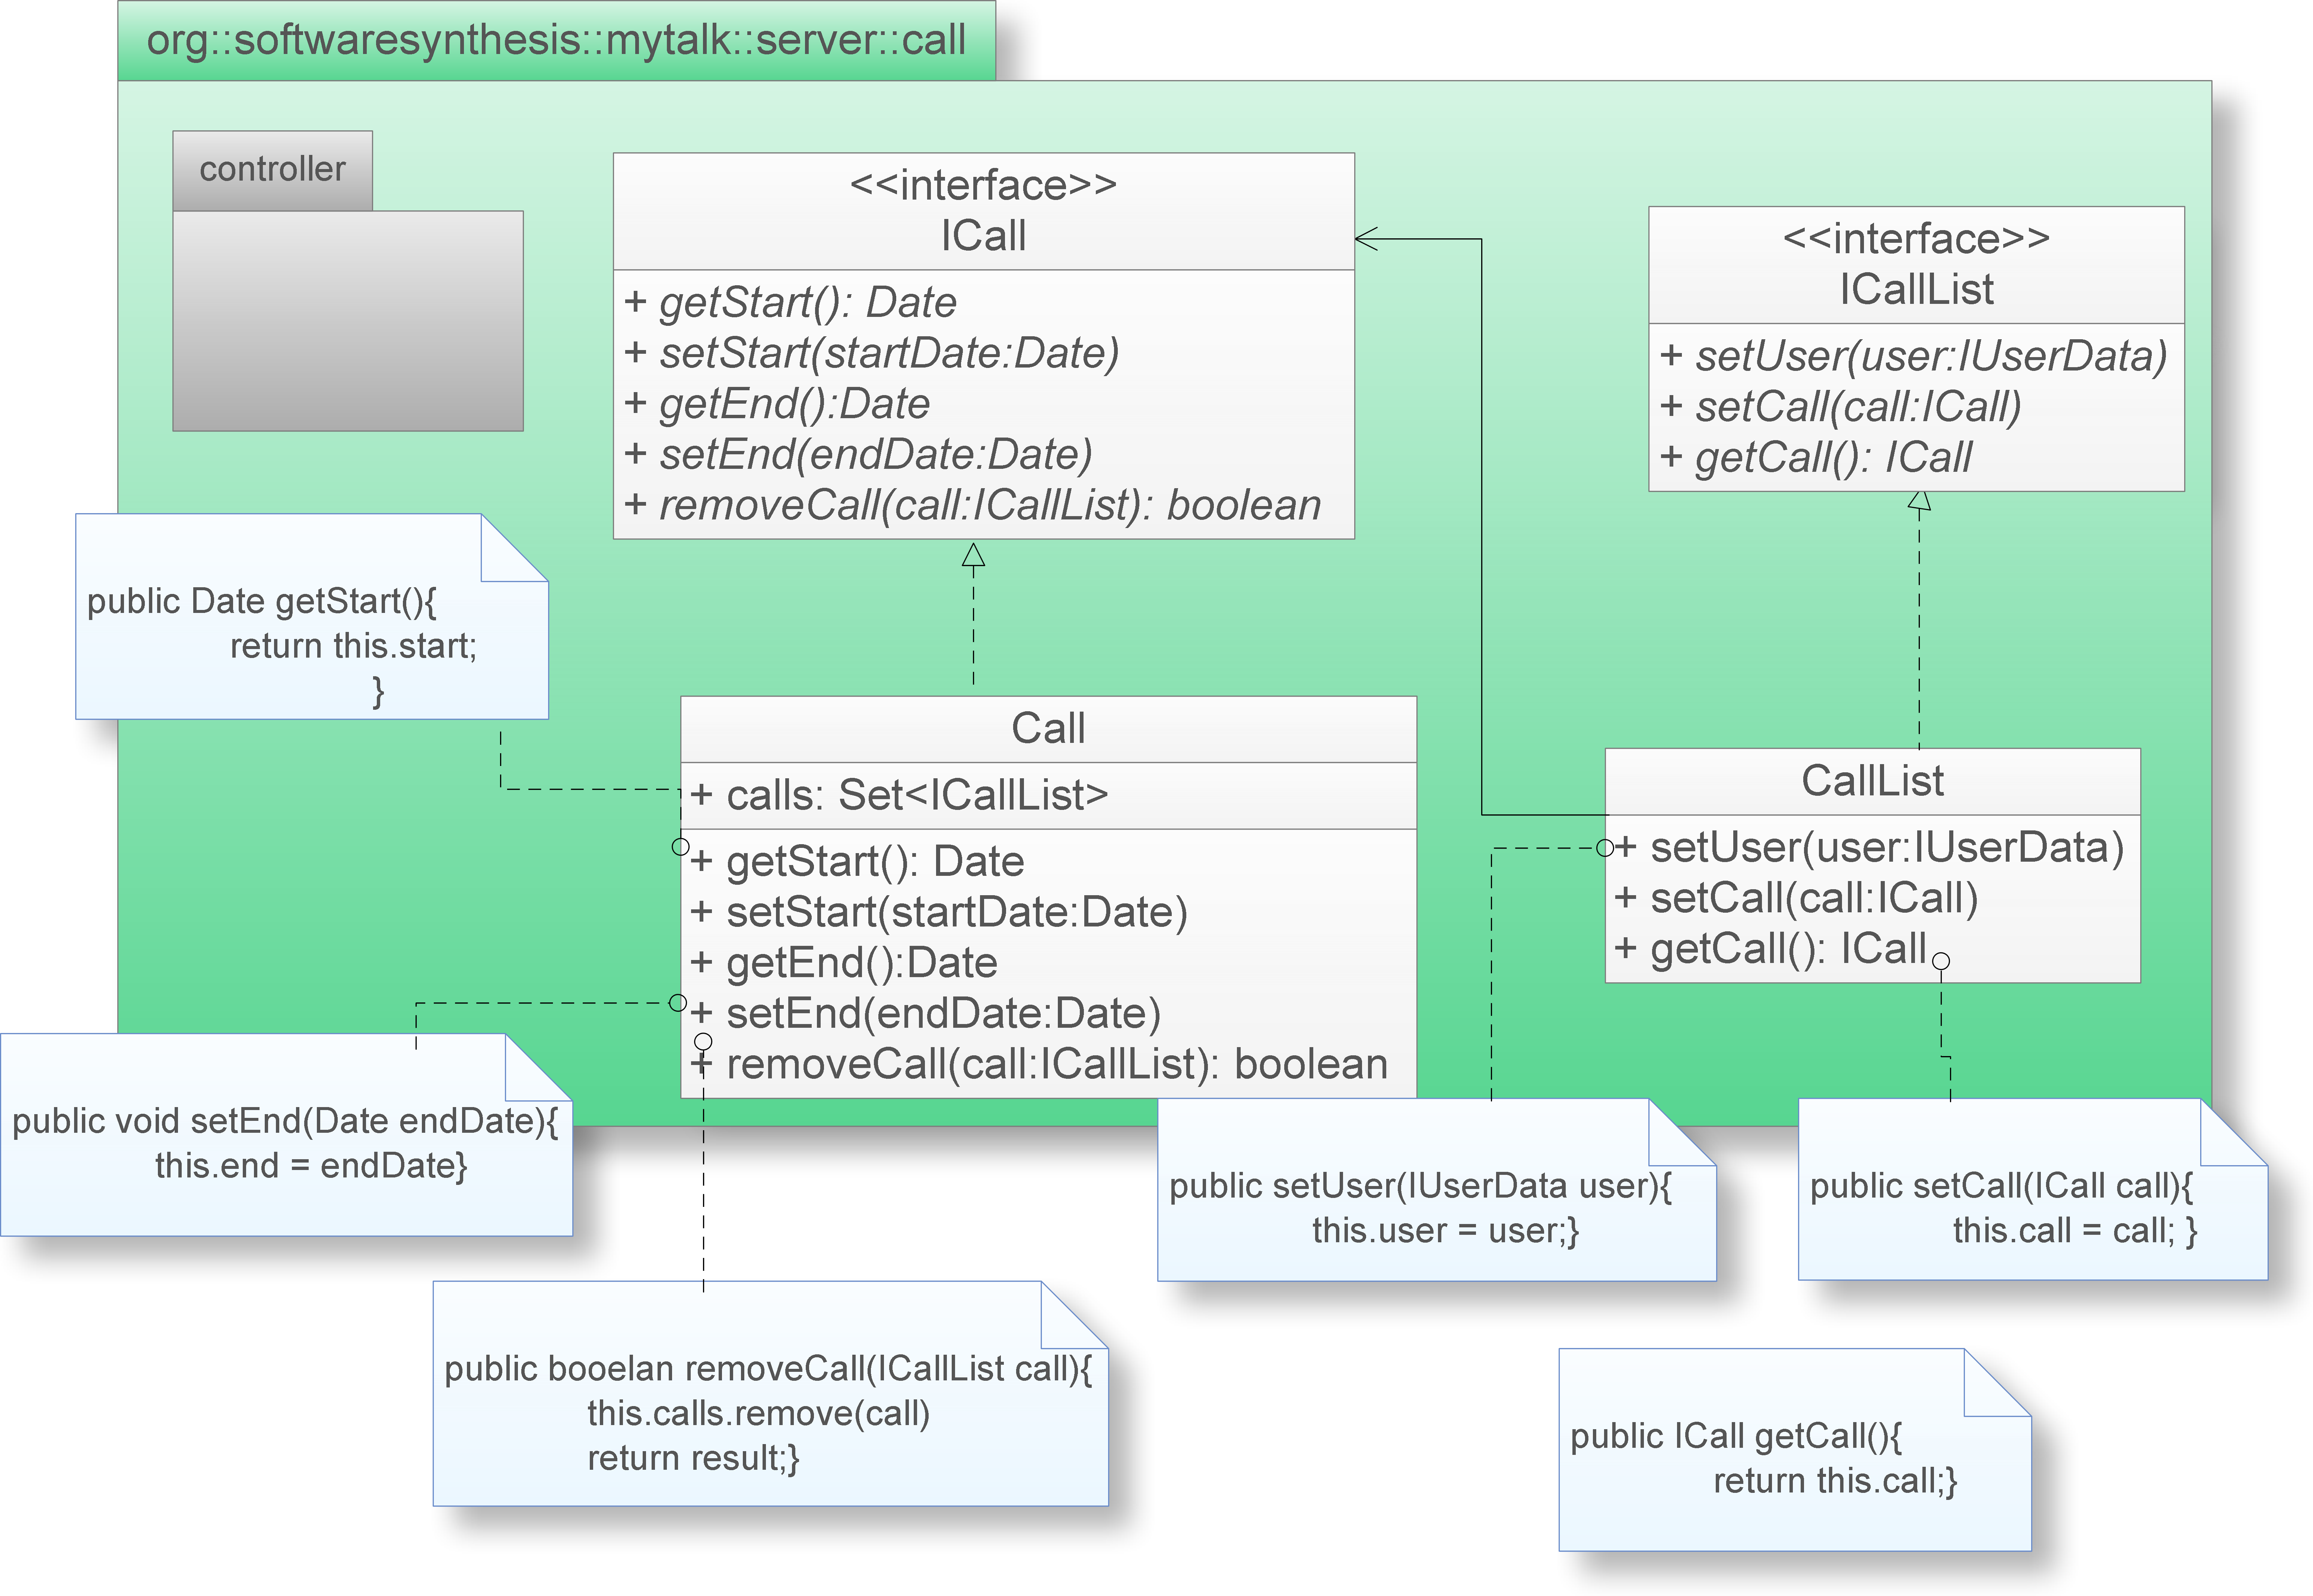
\includegraphics[width=\textwidth]{DDPCall}
\caption{Diagramma package server.call}
\end{figure}
\end{center}

\classsection{ICall}

\subsubsection*{Funzione}
Interfaccia che rappresenta una chiamata effettuata dal sistema \caName. Gli oggetti che implementano tale interfaccia vengono usati per rappresentare lo storico delle chiamate di un utente.

\subsubsection*{Relazioni d'uso}
\begin{itemize}
	\item \texttt{java.util.Date}: tipo utilizzato per definire la data d'inizio e fine di una chiamata.
\end{itemize}

\subsubsection*{Classi estese ed interfacce implementate}

\begin{itemize}
	\item \texttt{org.softwaresynthesis.mytalk.server.IMyTalkObject}: interfaccia estesa utilizzata per dire che la classe è da considerarsi come un \texttt{transfer object} gestito da Hibernate.
\end{itemize}

\subsubsection*{Metodi}
\begin{description}
	\item{\method{+ getId(): Long}}\\
	Restituisce l'identificativo univoco della chiamata.
	\item{\method{+ getStart(): Date}}\\
	Restituisce un istanza di \texttt{java.util.Date} di avvio della chiamata.
	\item{\method{+ setStart(startDate: Date): void}}\\
	Imposta la data di avvio della chiamata.
	\item{\method{+ getEnd(): Date}}\\
	Restituisce la data in cui termina la chiamata
	\item{\method{+ setEnd(endDate: Date): void}}\\
	Imposta la data in cui termina la chiamata.
	\item{\method{+ getCall(): Set<ICallList>}}\\
	Metodo usato per ottenere la lista dei partecipanti alla chiamata.
	\item{\method{+ setCall(callList: Set<ICallList>): void}}\\
	Metodo usato per impostare la lista dei partecipanti alla chiamata.
	\item{\method{+ addCall(call: ICallList): boolean}}\\
	Metodo usato per aggiungere un partecipante alla chiamata.
	\item{\method{+ removeCall(call: ICallList): boolean}}\\
	Metodo usato per rimuovere un partecipate alla chiamata 
\end{description}

\classsection{Call}

\subsubsection*{Funzione}
Classe che implementa l'interfaccia \classname{ICall}.

\subsubsection*{Relazioni d'uso}
\begin{itemize}
	\item \texttt{java.util.Date}: tipo utilizzato per definire la data d'inizio e fine di una chiamata.
\end{itemize}

\subsubsection*{Classi estese ed interfacce implementate}
\begin{itemize}
	\item \classname{ICall} interfacci d'implementazione.
\end{itemize}

\subsubsection*{Attributi}

\begin{itemize}
	\item{\memberdata{-- id: long}}
	Attributo contenente il codice identificativo della chiamata.
	\item{\memberdata{-- startDate: Date}}
	Attributo di tipo \texttt{java.util.Date} contenente la data (compresa l'ora) d'inizio della chiamata.
	\item{\memberdata{-- endDate: Date}}
	Attributo di tipo \texttt{java.util.Date} contenente la data (compresa l'ora) in cui la chiamata è terminata.
	\item{\memberdata{-- calls: Set<ICallList>}}
	Attributo usato per definire la lista dei partecipanti alla chiamata.
\end{itemize}

\subsubsection*{Metodi}
\begin{description}
	\item{\method{+ getId(): Long}}\\
	Restituisce l'identificativo univoco della chiamata ritornando il contenuto dell'attributo \memberdata{id}.
	\item{\method{+ getStart(): Date}}\\
	Restituisce il contenuto del campo \memberdata{startDate}.
	\item{\method{+ setStart(startDate: Date): void}}\\
	Imposta la data di avvio della chiamata, sovrascrivendo il contenuto \memberdata{startData}.
	\item{\method{+ getEnd(): Date}}\\
	Restituisce il contenuto del campo \memberdata{endDate}.
	\item{\method{+ setEnd(endDate: Date): void}}\\
	Imposta la data di avvio della chiamata, sovrascrivendo il contenuto \memberdata{endData}.
	\item{\method{+ getCall(): Set<ICallList>}}\\
	Restituisce il contenuto del campo \memberdata{calls}.
	\item{\method{+ setCall(callList: Set<ICallList>): void}}\\
	Metodo usato per impostare la lista dei partecipanti alla chiamata. Sovrascrive il contenuto di \memberdata{calls}.
	\item{\method{+ addCall(call: ICallList): boolean}}\\
	Metodo usato per aggiungere un partecipante alla chiamata. Aggiunge al \memberdata{calls} un nuovo partecipante (call). Il metodo termina ritornando \texttt{true} se l'operazione va a buon fine, \texttt{false} altrimenti.
	\item{\method{+ removeCall(call: ICallList): boolean}}\\
	Metodo usato per rimuovere un partecipate alla chiamata, esso avviene invocando il metodo \texttt{remove(call)} dall'attributo \memberdata{calls}. Il metodo ritorna un valore booleano per indicare l'esisto dell'operazione: \texttt{false} in presenza di errori, \texttt{true} altrimenti.
\end{description}

\classsection{ICallList}

\subsubsection*{Funzione}
Interfaccia rappresentante una \textit{entry} di uno storico chiamate di un utente del sistema \caName.

\subsubsection*{Relazioni d'uso}
\begin{itemize}
	\item \classname{IUserData}: l'interfaccia \classname{ICallList} definisce più metodi che restituiscono oggetti aventi tipo di ritorno \classname{IUserData}, essi sono i metodi \inglese{get} per ottenere l'utente che ha effettuato la chiamata. Analogamente \classname{IUserData} viene usato come parametro d'ingresso per i metodi \inglese{set} collegati ai metodi già citati.
	\item \classname{ICall}: l'interfaccia \classname{ICallList} definiscono metodi che restituiscono oggetti aventi tipo di ritorno \classname{ICall}.
\end{itemize}

\subsubsection*{Classi estese ed interfacce implementate}
\begin{itemize}
	\item \texttt{org.softwaresynthesis.mytalk.server.IMyTalkObject}: interfaccia da estendere. Ogni oggetto che implementerà l'interfaccia \classname{ICallList} dovrà essere in grado di convertire il proprio contenuto informativo in formato JSON.
\end{itemize}

\subsubsection*{Metodi}
\begin{description}
	\item{\method{+ getId(): Long}}\\
	Restituisce l'identificativo univoco di una \inglese{entry} di uno storico chiamate.
	
	\item{\method{+ setIdCall(call: ICall): void}}\\
	Imposta l'id della chiamta \classname{ICall} (passato come parametro d'ingresso).
	\item{\method{+ getIdCall(): IUserData}}\\
	Restituisce un id di un oggetto avente tipo \classname{ICall} rappresentante una chiamata effettuata dall'utente.
	
	\item{\method{+ setIdUser(contact: IUserData): void}}\\
	Imposta l'id dell'utente \classname{IUserData} (passato come parametro d'ingresso) come l'utente che ha effettuato la chiamata.
	\item{\method{+ getIdUser(): IUserData}}\\
	Restituisce l'id di oggetto avente tipo \classname{IUserData} rappresentante l'utente che ha effettuato la chiamata.
	
	\item{\method{+ setCaller(caller: boolean): void}}\\
	Imposta l'utente che ha effettuato la chiamata come chiamante se il parametro ricevuto ha valore \texttt{true}.
	\item{\method{+ getCaller(): boolean}}\\
	Ritorna un valore di tipo \texttt{bool} se l'utente della chiamata è colui che l'ha iniziata o meno.
\end{description}




\classsection{CallList}

\subsubsection*{Funzione}
Classe che implementa l'interfaccia \classname{ICallList}.

\subsubsection*{Relazioni d'uso}

Nessuna relazione evidenziata.

\subsubsection*{Classi estese ed interfacce implementate}
\begin{itemize}
	\item \texttt{call.ICallList}: interfaccia implementata dalla classe.
\end{itemize}

\subsubsection*{Attributi}

\begin{itemize}
	\item{\memberdata{-- id: long}}
	Attributo contenente il codice identificativo dello storico chiamata.
	\item{\memberdata{-- idCall: long}}
	Attributo contenente il codice identificativo della chiamata.
	\item{\memberdata{-- idUser: long}}
	Attributo contenente il codice identificativo dell'utente partecipante alla chiamata.
	\item{\memberdata{-- caller: boolean}}
	Attributo che identifica se l'utente è il chiamante o meno.
\end{itemize}

\subsubsection*{Metodi}
\begin{description}
	\item{\method{+ getId(): Long}}\\
	Restituisce il valore dell'attributo \memberdata{id}.
	
	\item{\method{+ setIdCall(call: Long): void}}\\
	Imposta il valore dell'attributo \memberdata{idCall} con il valore ricevuto da parametro ``call''.
	\item{\method{+ getIdCall(): Long}}\\
	Restituisce il valore dell'attributo \memberdata{idCall}.
	
	\item{\method{+ setIdUser(contact: Long): void}}\\
	Imposta il valore dell'attributo \memberdata{idUser} con il valore ricevuto da parametro ``contact''.
	\item{\method{+ getIdUser(): Long}}\\
	Restituisce il valore dell'attributo \memberdata{idUser}.
	
	\item{\method{+ setCaller(caller: boolean): void}}\\
	Imposta il valore dell'attributo \memberdata{caller} con il valore ricevuto da parametro ``caller''.
	\item{\method{+ getCaller(): boolean}}\\
	Restituisce il valore dell'attributo \memberdata{caller}.
\end{description}

\subsection{Package \texttt{org.softwaresynthesis.mytalk.server.call.controller}}\label{sec:callServlet}

\begin{center}
\begin{figure}[H]
  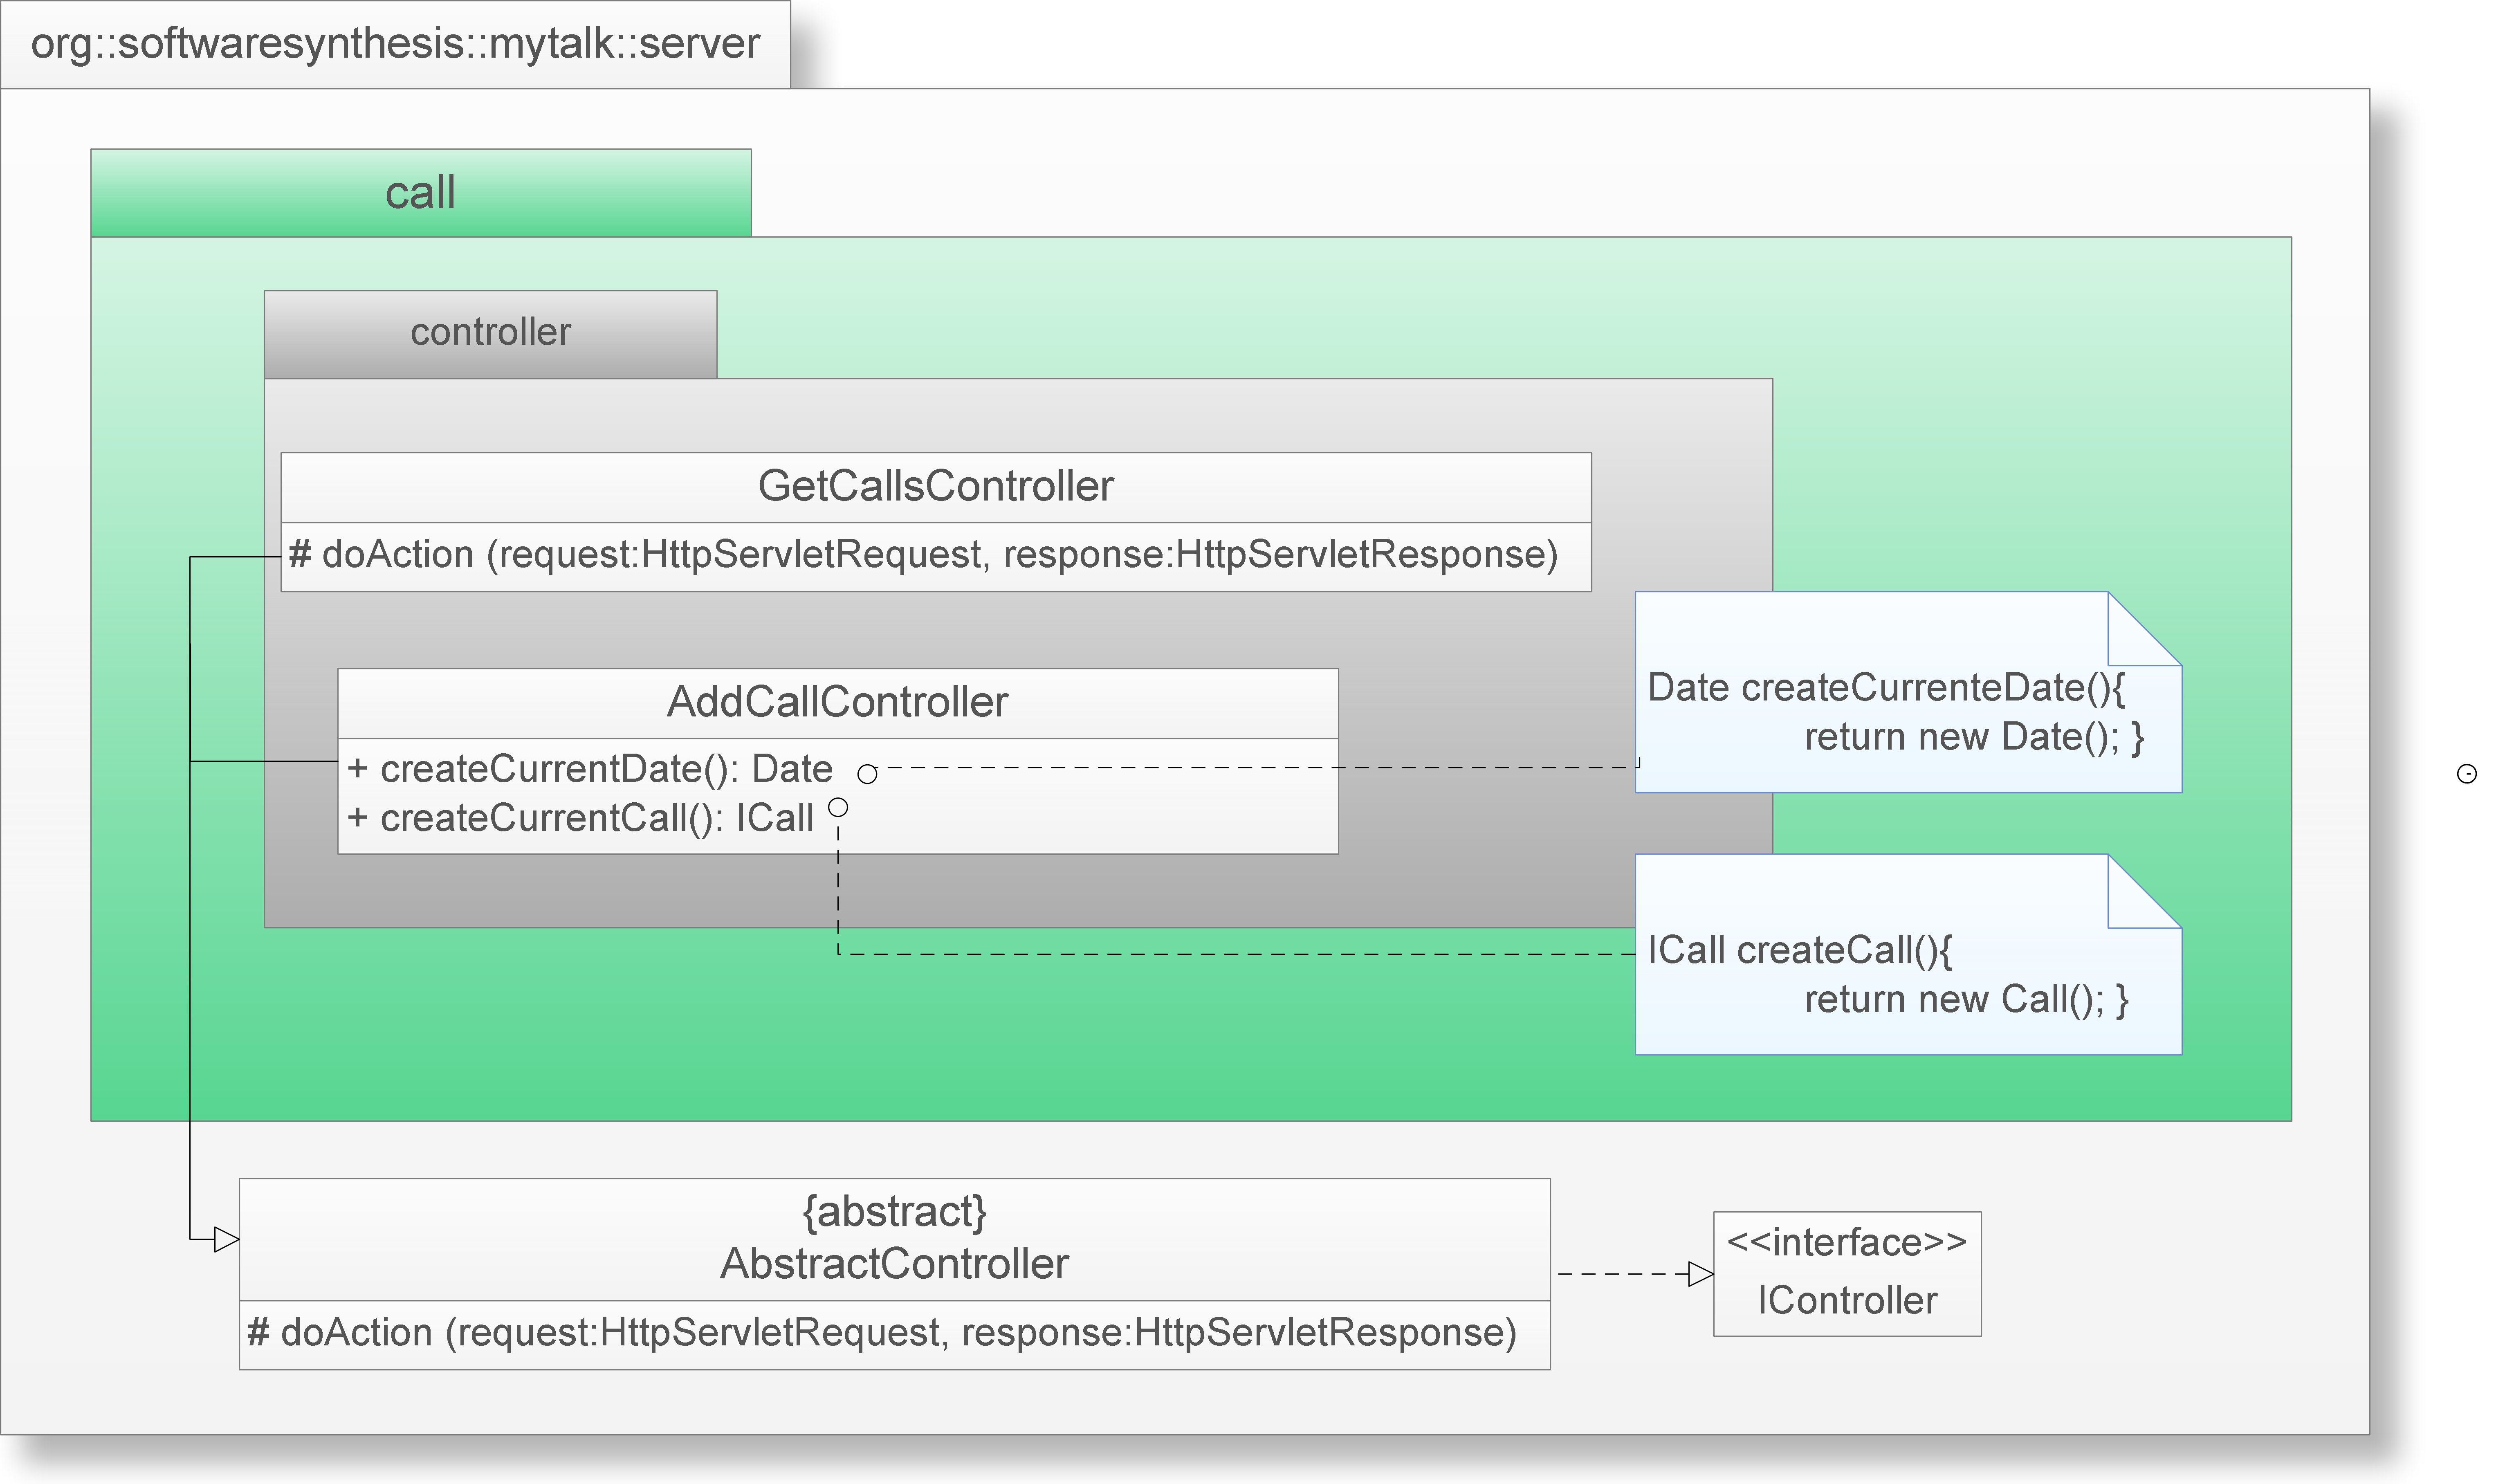
\includegraphics[width=\textwidth]{DDPCallController}
\caption{Diagramma package server.call.controller}
\end{figure}
\end{center}

\classsection{GetCallsController}

\subsubsection*{Funzione}
\textit{Controller} da richiamare per effettuare il download della lista che rappresenta lo storico delle chiamate effettuate e ricevute dell'utente. I dati vengono ritornati sotto forma di stringa in formato JSON.

\subsubsection*{Relazioni d'uso}
\begin{itemize}
	\item \texttt{java.io.IOException}: eccezione richiamabile dal metodo\method{doAction()}.
	\item \texttt{java.io.PrintWriter}: classe istanziata all'interno del metodo \method{doAction()}. Usata per scrivere l'output del controller.
	\item \texttt{javax.servlet.ServletException}: eccezione sollevabile dai metodi \method{doAction()}.
	\item \texttt{javax.servlet.http.HttpServletRequest}: classe usata per interagire con le richieste AJAX inoltrate dal client.
	\item \texttt{javax.servlet.http.HttpServletResponse}: classe usata per interagire con le richieste AJAX inoltrate dal client.
	\item \classname{call.ICall}: usata per definire un oggetto rappresentante una chiamata.
	\item \classname{abook.IUserData}: usata per definire un utente generico, che ha partecipato alla chiamata.
\end{itemize}

\subsubsection*{Classi estese ed interfacce implementate}
\begin{itemize}
	\item \texttt{server.AbstractController}: classe estesa.
\end{itemize}

\subsubsection*{Attributi}

Nessun attributo evidenziato

\subsubsection*{Metodi}
\begin{description}
	
	\item{\method{\# doAction(request: HttpServletRequest, response: HttpServletResponse): void}}\\
	Metodo usato per accedere alla funzionalità del \textit{controller}. Il procedimento da definire passa attraverso 3 step essenziali:
	\begin{itemize}
		\item \texttt{Inizializzazione}: si imposta la variabile user nel seguente modo:
			\begin{itemize}
				\item si procede salvando l'indirizzo mail in una stringa (mail). Tale indirizzo è ottenuto mediante una chiamata a \method{getUserMail()};
				\item si esegue una chiamata a \texttt{userDAO.getUserData(mail)}, il cui valore restituito viene in fine salvato in user;
			\end{itemize}
		\item \texttt{Elaborazione dati}: il metodo interroga il database attraverso la classe \classname{DataPersistanceManager}. Per ogni oggetto \classname{ICall} in cui si evidenzia che uno dei due partecipanti è il client (\classname{IUserData}) che ha inoltrato la richiesta al \textit{front controller}, si aggiunge alla stringa \texttt{result} da ritornare i dati di tale chiamata. Nello specifico la formattazione della stringa di ritorno, dovrà descrivere la seguente logica:\\
		
		\verb|{name:"NOME_UTENTE",start="DATA_INIZIO",end="DATA_FINE"}|\\
		
		Si consideri che la dove vi è un nome in maiuscolo, vi dovrà essere il dato inerente estrapolato dall'istanza \classname{ICall} presa in considerazione.
		\item \texttt{Restituzione risultato}: dopo aver elaborato i dati, il \textit{controller} dovrà scrivere nel \texttt{PrintWriter} associato alla \textit{request}:
			\begin{itemize}
				\item una stringa formattata come sopra, se l'utente ha effettuato o ricevuto almeno una chiamata;
				\item \texttt{null}, altrimenti.
			\end{itemize}
	\end{itemize}

\end{description}

\classsection{AddCallController}

\subsubsection*{Funzione}
\textit{Controller} da richiamare per aggiungere una nuova chiamata al database.

\subsubsection*{Relazioni d'uso}
\begin{itemize}
	\item \texttt{java.io.IOException}: eccezione richiamabile dal metodo\method{doAction()}.
	\item \texttt{java.io.PrintWriter}: classe istanziata all'interno del metodo \method{doAction()}. Usata per scrivere l'output del \inglese{controller}.
	\item \texttt{javax.servlet.ServletException}: eccezione sollevabile dai metodi \method{doAction()}.
	\item \texttt{javax.servlet.http.HttpServletRequest}: classe usata per interagire con le richieste AJAX inoltrate dal client.
	\item \texttt{javax.servlet.http.HttpServletResponse}: classe usata per interagire con le richieste AJAX inoltrate dal client.
	\item \classname{call.ICall}: usata per definire un oggetto rappresentante una chiamata.
	\item \classname{abook.IUserData}: usata per definire un utente generico, che ha partecipato alla chiamata.
\end{itemize}

\subsubsection*{Classi estese ed interfacce implementate}
\begin{itemize}
	\item \texttt{server.AbstractController}: classe estesa.
\end{itemize}

\subsubsection*{Attributi}

Nessun attributo evidenziato

\subsubsection*{Metodi}
\begin{description}
	
	\item{\method{\# doAction(request: HttpServletRequest, response: HttpServletResponse): void}}\\
	Metodo usato per accedere alla funzionalità del \textit{controller}. Il metodo può essere pensato come suddiviso in due parti logiche: la creazione delle variabili locali, e il blocco \textit{try-catch} di esecuzione delle istruzioni di aggiunta al database. Nella prima parte il metodo definisce le seguenti variabili (NOTA: il nome usato non può essere cambiato a piacere, ma deve essere quello qui prestabilito):
	
	\begin{itemize}
		\item Long userId = null;
		\item String email = null;
		\item IUserData user = null;
		\item IUserData other = null;
		\item ICall call = null;
		\item ICallList userCall = null;
		\item ICallList otherCall = null;
		\item Date date = null;
		\item Writer writer = null;
		\item DataPersistanceManager dao = null;
		\item String result = null;
	\end{itemize}

Dopo questa fase di inizializzazione, il metodo definisce un blocco \textit{try-catch}. Il \textit{catch} definito cattura un eccezione generica di tipo \texttt{Exception} e si occupa semplicemente di impostare \texttt{result} a \texttt{null} (si sottolinea che \texttt{result} è la stringa da ritornare nel \texttt{writer} per informare il chiamante sul risultato della chiamata a metodo). Inoltre è definito un blocco \textit{finaly} che si occupa di inizializzare \texttt{writer} a partire da \texttt{response.getWriter()}. Quindi termina scrivendo nel \texttt{writer} il contenuto della stringa \texttt{result}.

Tornando al blocco \textit{try}, in esso si evidenziano i seguenti step:

\begin{itemize}
	\item si impostano le variabili locali legate al contenuto informativo della chiamata (email, userId, user, other, date, call) con i dati ottenuti da apposite chiamate all'istanza di \classname{DataPersistanceManager};
	\item si inserisce la chiamata cosi creata attraverso un istruzione \texttt{dao.insert(call)};
	\item si inserisce la prima \texttt{CallList} associata, definendo una nuova CallList da memorizzare in userCall. Quindi si imposta il suo contenuto con \texttt{call} e \texttt{user} e si termina questo step aggiungendo \texttt{userCall} al contenuto del database (usare sempre una chiamata a metodo \texttt{dao.insert(userCall)};
	\item si inserisce la seconda \texttt{CallList}. La procedura è identica a quella dello step precedente, con la differenza che  al posto di user si usa other per impostare il campo utente della chiamata;
	\item il blocco \textit{try} termina impostando \texttt{result} a \texttt{true}.
\end{itemize}

\end{description}

\subsection{Package \texttt{org.softwaresynthesis.mytalk.server.message}}\label{sec:message}

\begin{center}
\begin{figure}[H]
  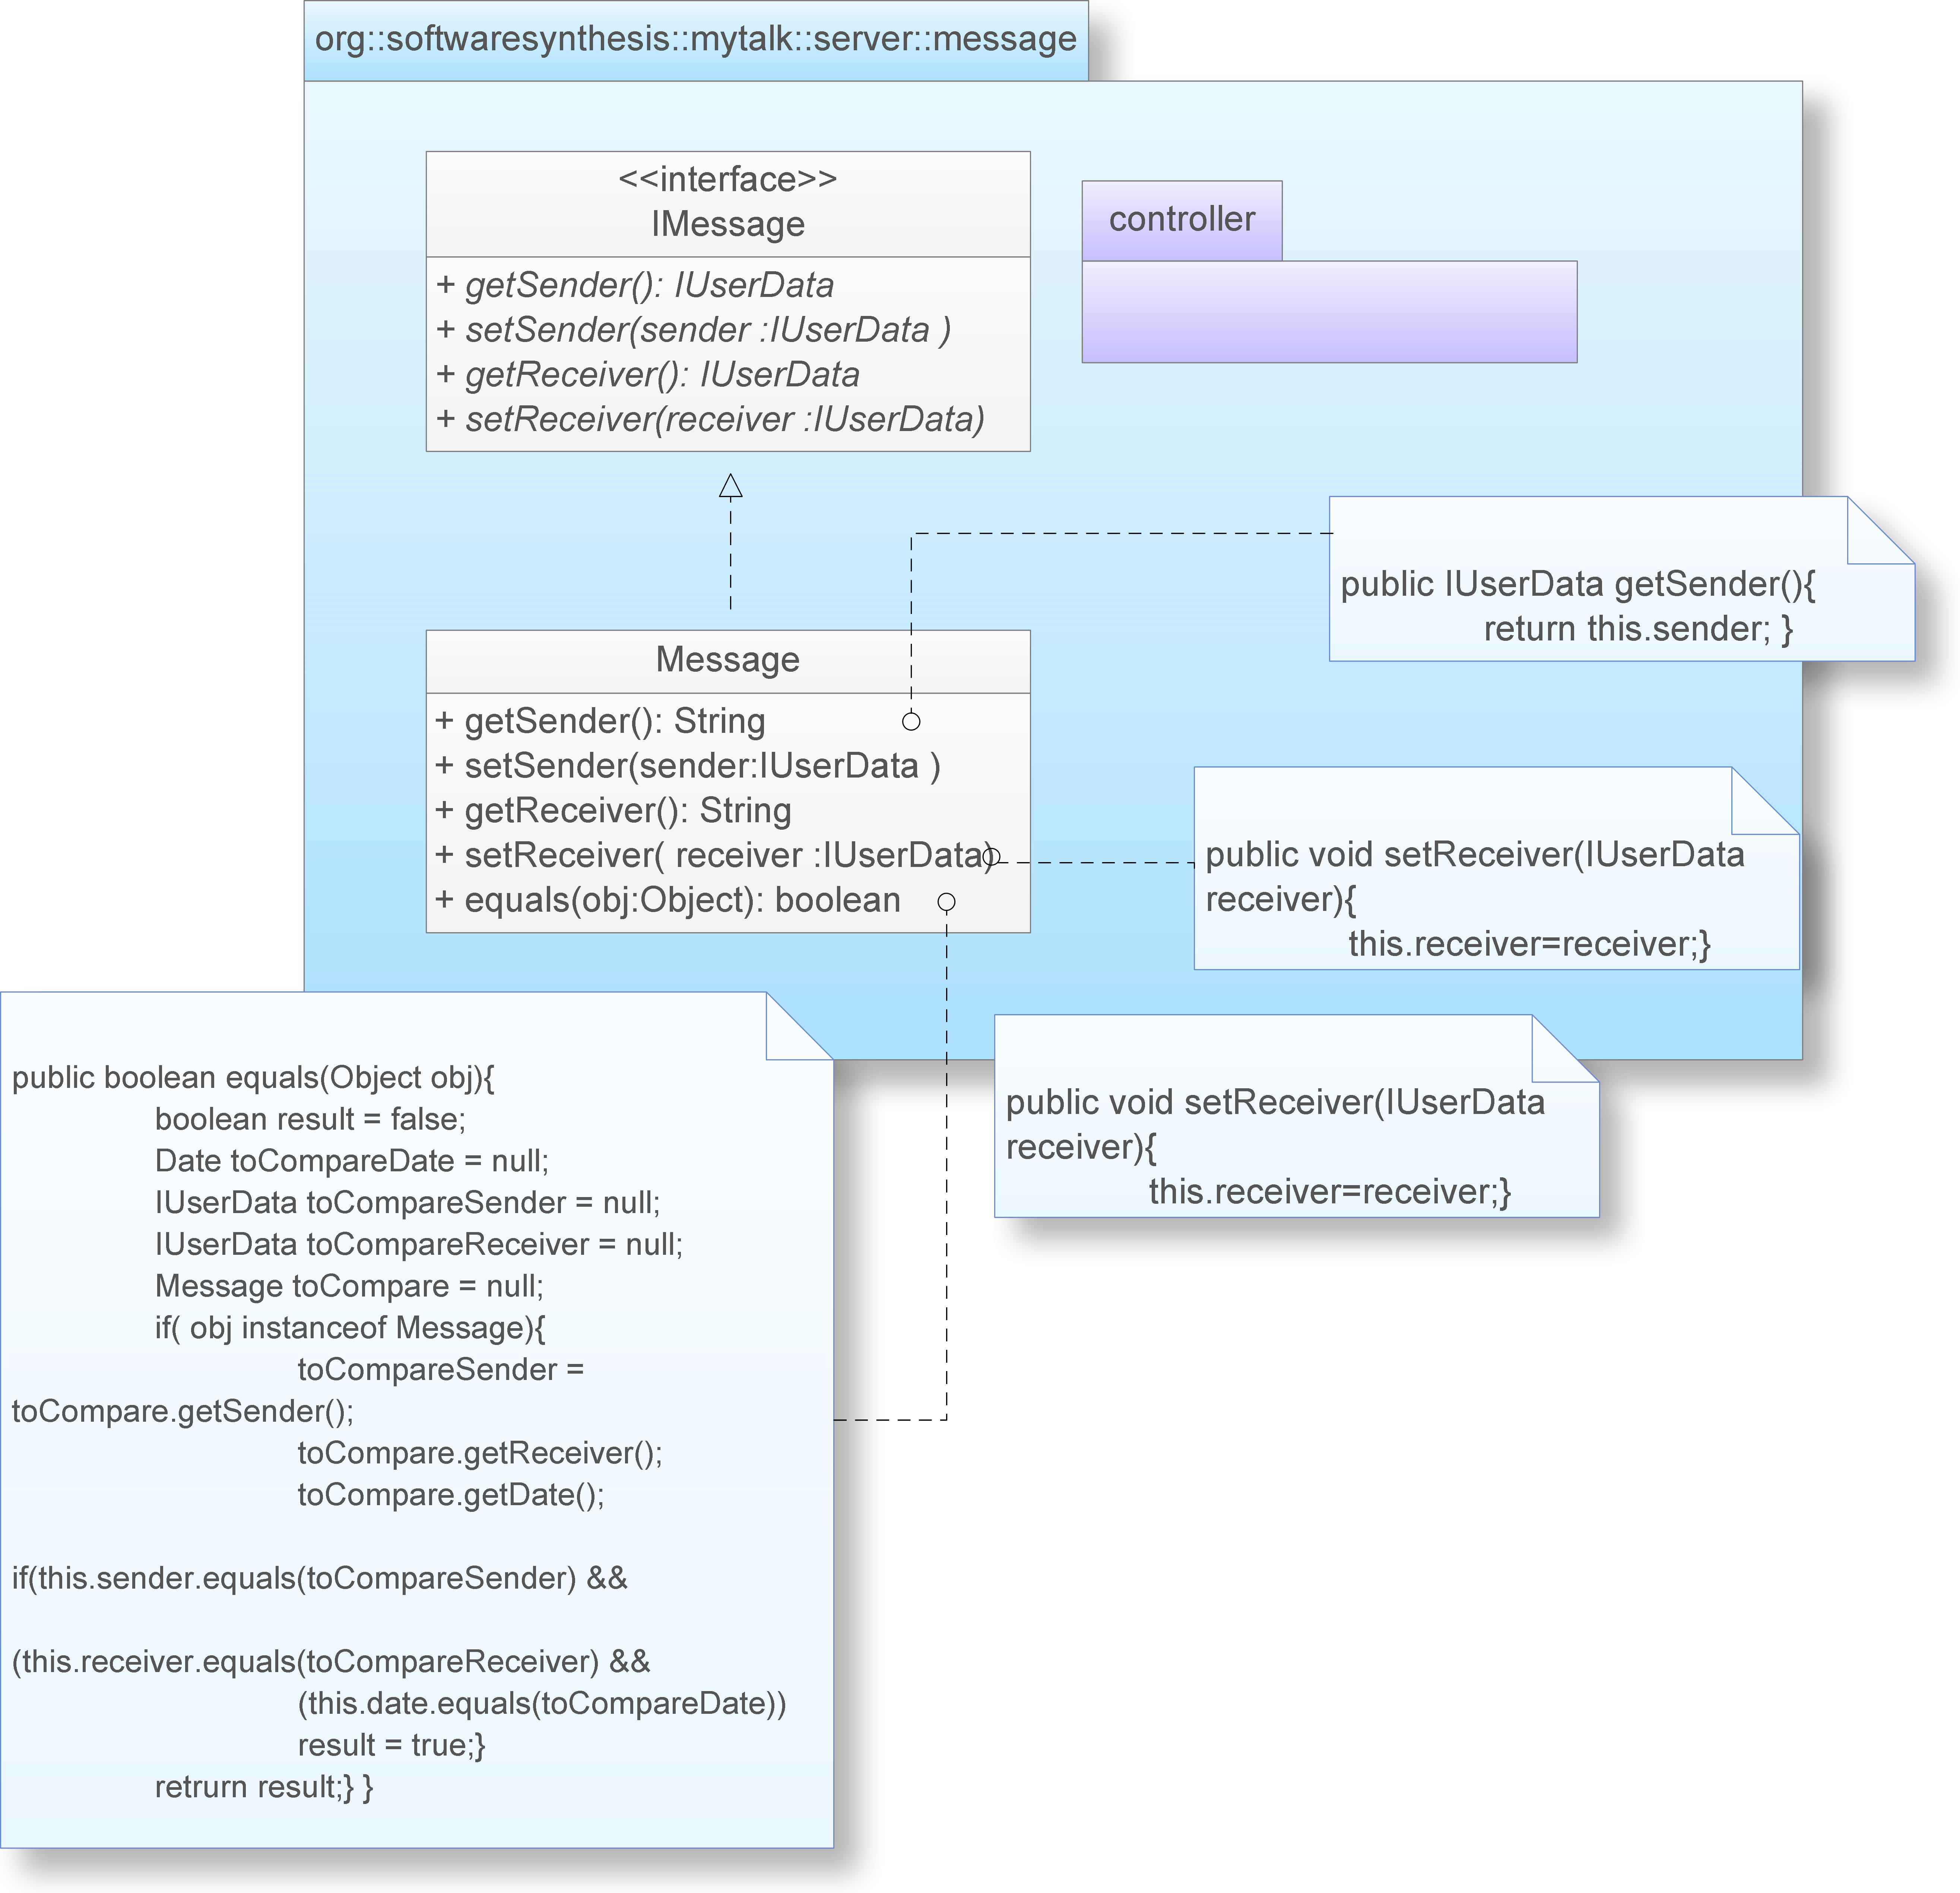
\includegraphics[width=\textwidth]{DDPMessage}
\caption{Diagramma package server.message}
\end{figure}
\end{center}


\classsection{IMessage}

\subsubsection*{Funzione}
Interfaccia che rappresenta un messaggio di segreteria del sistema \caName.

\subsubsection*{Relazioni d'uso}
\begin{itemize}
	\item \texttt{java.util.Date}: tipo utilizzato per definire la data in cui è stato registrato un messaggio.
	\item \classname{abook.IUserData}: usata per rappresentare il mittente e il destinatario del messaggio di segreteria.
\end{itemize}

\subsubsection*{Classi estese ed interfacce implementate}

\begin{itemize}
	\item \texttt{org.softwaresynthesis.mytalk.server.IMyTalkObject}: interfaccia estesa. Utilizzata per dire che la classe è da considerarsi come un \texttt{transfer object} gestito da Hibernate.
\end{itemize}

\subsubsection*{Metodi}
\begin{description}
	\item{\method{+ getId(): Long}}\\
	Restituisce l'identificativo univoco del messaggio.
	\item{\method{+ getSender(): IUserData}}\\
	Restituisce un istanza di tipo classname{abook.IUserData} che rappresenta il mittente del messaggio.
	\item{\method{+ setSender(sender: IUserData): void}}\\
	Imposta il mittente del messaggio.
	\item{\method{+ getReceiver(): IUserData}}\\
	Restituisce un istanza di tipo classname{abook.IUserData} che rappresenta il destinatario del messaggio.
	\item{\method{+ setReceiver(receiver: IUserData): void}}\\
	Imposta il destinatario del messaggio.
	\item{\method{+ getNewer(): boolean}}\\
	Restituisce un valore booleano che identifica lo stato del messaggio (``già letto'' se il valore ritornato è \texttt{true}, ``da leggere'' se il valore ritornato è \textit{false}).
	\item{\method{+ setNewer(status: boolean): void}}\\
	Imposta il messaggio come ``già ascoltato'' o come ``da ascoltare''.
	\item{\method{+ getVideo(): boolean}}\\
	Restituisce un booleano che determina se si tratta di un messaggio audio oppure audio-video.
	\item{\method{+ setVideo(video: boolean): void }}\\	
	Imposta il messaggio come messaggio audio-video o come messaggio contenente solamente una traccia audio.
	\item{\method{+ getDate(): Date}}\\
	Restituisce la data in cui il mittente ha lasciato il messaggio nella segreteria del destinatario.
	\item{\method{+ setDate(date: Date): void}}\\
	Imposta la data in cui il mittente ha lasciato il messaggio nella segreteria del destinatario.
\end{description}

\classsection{Message}

\subsubsection*{Funzione}
Classe che implementa l'interfaccia \classname{IMessage}.

\subsubsection*{Relazioni d'uso}
\begin{itemize}
	\item \texttt{java.util.Date}: tipo utilizzato per definire la data in cui è stato registrato un messaggio.
	\item \classname{abook.IUserData}: usata per rappresentare il mittente e il destinatario del messaggio di segreteria.
\end{itemize}

\subsubsection*{Classi estese ed interfacce implementate}
\begin{itemize}
	\item \classname{message.IMessage}: interfaccia d'implementazione.
\end{itemize}

\subsubsection*{Attributi}

\begin{itemize}
	\item{\memberdata{-- id: long}}
	Attributo contenente il codice identificativo del messaggio.
	\item{\memberdata{-- sender: IUserData}}
	Attributo contenente lo \classname{IUserData} che rappresenta il destinatario del messaggio.
	\item{\memberdata{-- receiver: IUserData}}
	Attributo contenente lo \classname{IUserData} che rappresenta il destinatario del messaggio.
	\item{\memberdata{-- status: boolean}}
	Attributo contenente un valore booleano che identifica se il messaggio è stato visionato/ascoltato o meno. L'attributo se impostato a \texttt{true}, designa il messaggio come \textit{ascoltato}. Invece se impostato a \texttt{false} identifica il messaggio come \textit{ancora da ascoltare}.
	\item{\memberdata{-- video: boolean}}
	Attributo che stabilisce se il messaggio contiene o meno una traccia video. Si ricorda che ogni messaggio contiene (di \inglese{default}) una traccia audio. Se tale attributo è impostato a \texttt{true} allora il messaggio contiene una traccia video.
	\item{\memberdata{-- date: Date}}
	Attributo che definisce l'orario di invio del messaggio.
\end{itemize}

\subsubsection*{Metodi}
\begin{description}
	\item{\method{+ getId(): Long}}\\
	Restituisce l'identificativo univoco del messaggio, ritornando il contenuto di \memberdata{id}.
	\item{\method{+ getSender(): IUserData}}\\
	Restituisce un istanza di tipo classname{abook.IUserData} che rappresenta il mittente del messaggio. Nello specifico il metodo ritorna l'attributo \memberdata{sender}.
	\item{\method{+ setSender(sender: IUserData): void}}\\
	Imposta il mittente del messaggio, sovrascrivendo il contenuto dell'attributo \memberdata{sender}.
	\item{\method{+ getReceiver(): IUserData}}\\
	Restituisce un istanza di tipo classname{abook.IUserData} che rappresenta il destinatario del messaggio. Nello specifico il metodo ritorna l'attributo \memberdata{receiver}.
	\item{\method{+ setReceiver(receiver: IUserData): void}}\\
	Imposta il destinatario del messaggio, sovrascrivendo il contenuto dell'attributo \memberdata{receiver}.
	\item{\method{+ getNewer(): boolean}}\\
	Metodo che ritorna il contenuto dell'attributo \memberdata{status}.
	\item{\method{+ setNewer(status: boolean): void}}\\
	Imposta il messaggio come ``già ascoltato'' o come ``da ascoltare'', sovrascrivendo il contenuto dell'attributo \memberdata{status}.
	\item{\method{+ getVideo(): boolean}}\\
	Restituisce il contenuto dell'attributo \memberdata{video}.
	\item{\method{+ setVideo(video: boolean): void }}\\	
	Metodo usato per impostare la ``natura'' del messaggio, impostando il contenuto dell'attributo \memberdata{video} mettendolo a \texttt{true} se il messaggio contiene una traccia video, oppure a \texttt{false} se non la contiene.
	\item{\method{+ getDate(): Date}}\\
	Restituisce la data in cui il mittente ha lasciato il messaggio nella segreteria del destinatario, ritornando il contenuto dell'attributo \memberdata{date}.
	\item{\method{+ setDate(date: Date): void}}\\
	Imposta la data in cui il mittente ha lasciato il messaggio nella segreteria del destinatario, sovrascrivendo il contenuto dell'attributo \memberdata{date}.

\end{description}

\subsection{Package \texttt{org.softwaresynthesis.mytalk.server.message.controller}}\label{sec:messageServlet}

\begin{center}
\begin{figure}[H]
  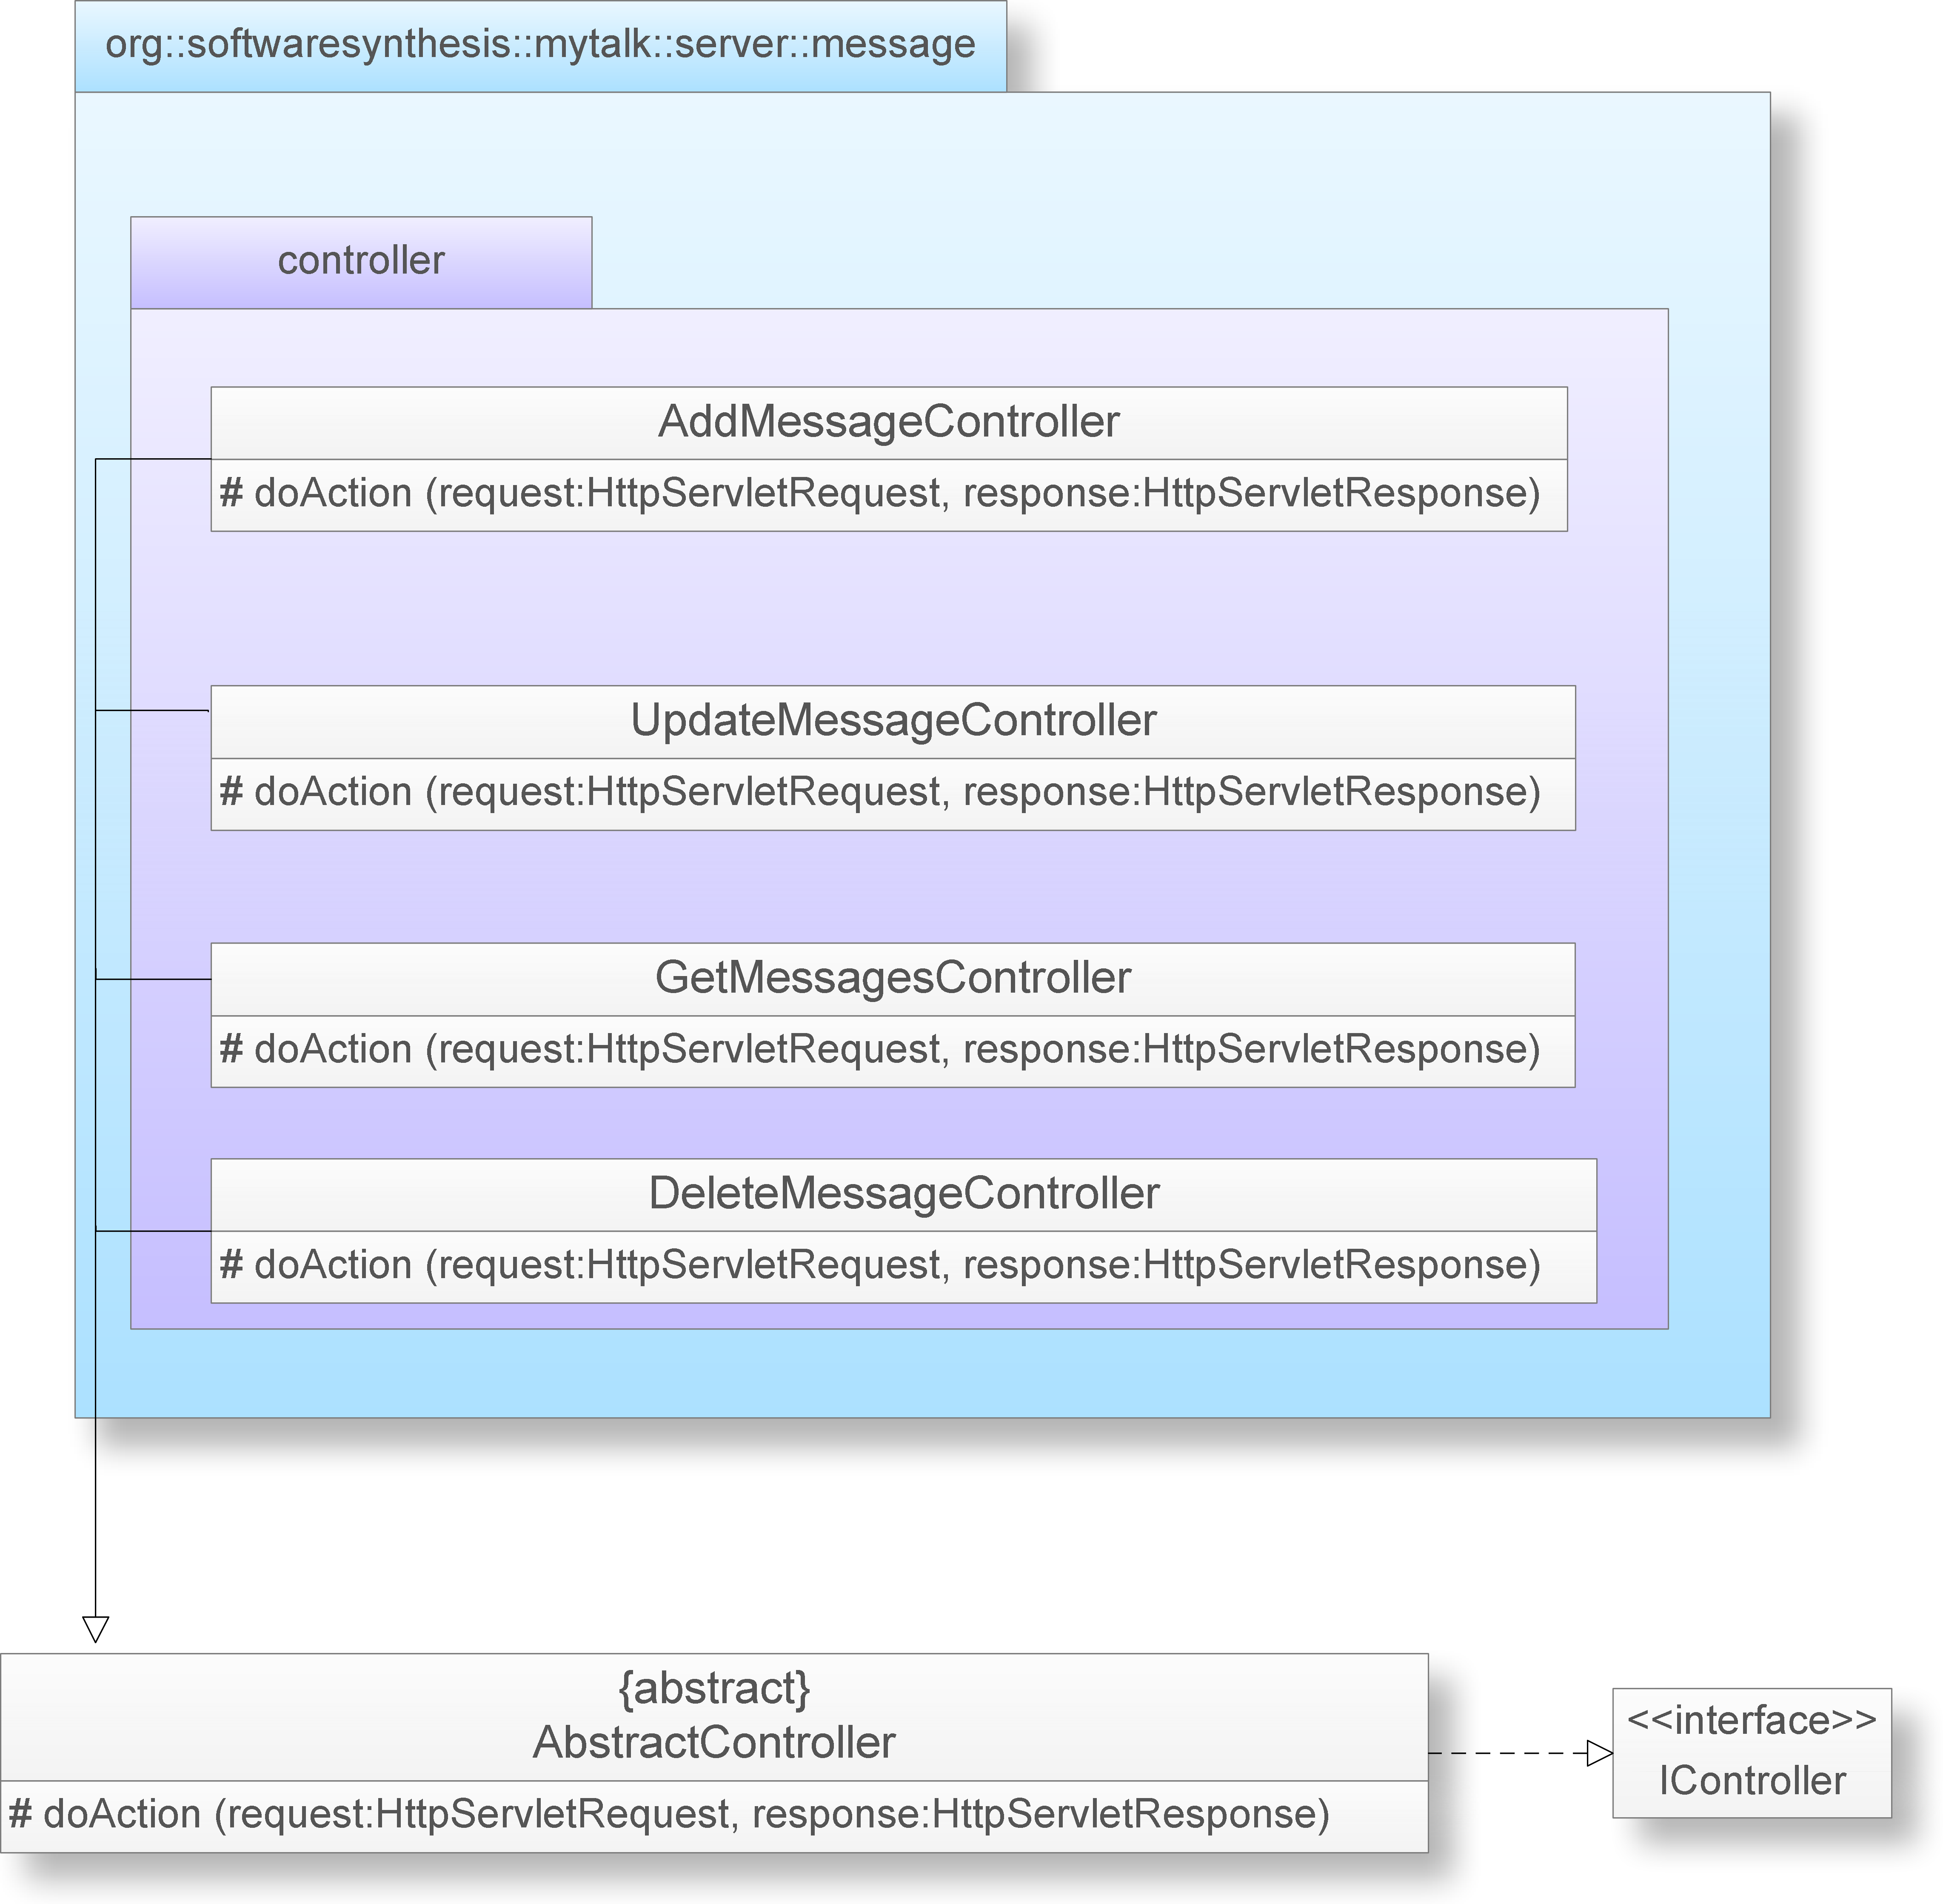
\includegraphics[width=\textwidth]{DDPMessageController}
\caption{Diagramma package server.message.controller}
\end{figure}
\end{center}

\classsection{AddMessageController}

\subsubsection*{Funzione}
\inglese{Controller} da richiamare per inserire un messaggio nella segreteria di un utente.

\subsubsection*{Relazioni d'uso}
\begin{itemize}
	\item \texttt{java.io.IOException}: eccezione richiamabile dal metodo\method{doAction()}.
	\item \texttt{java.io.PrintWriter}: classe istanziata all'interno del metodo \method{doAction()}. Usata per scrivere l'output della del \inglese{controller}.
	\item \texttt{javax.servlet.ServletException}: eccezione sollevabile dai metodi \method{doAction()}.
	\item \texttt{javax.servlet.http.HttpServletRequest}: classe usata per interagire con le richieste AJAX inoltrate dal client.
	\item \texttt{javax.servlet.http.HttpServletResponse}: classe usata per interagire con le richieste AJAX inoltrate dal client.
	\item \classname{message.IMessage}: usata per definire un oggetto rappresentante un messaggio in segreteria.
	\item \classname{abook.IUserData}: usata per definire un utente generico, che ha partecipato alla chiamata.
\end{itemize}

\subsubsection*{Classi estese ed interfacce implementate}
\begin{itemize}
	\item \texttt{server.AbstractController}: classe estesa.
\end{itemize}

\subsubsection*{Attributi}

Nessun attributo evidenziato

\subsubsection*{Metodi}
\begin{description}
	
	\item{\method{\# doAction(request: HttpServletRequest, response: HttpServletResponse): void}}\\
	Metodo usato per accedere alla funzionalità del controller. Il procedimento da definire passa attraverso 3 step essenziali:
	\begin{itemize}
		\item \texttt{Inizializzazione}: si imposta la variabile user nel seguente modo:
			\begin{itemize}
				\item si procede salvando l'indirizzo mail in una stringa (mail). Tale indirizzo è ottenuto mediante una chiamata a \method{getUserMail()};
				\item si esegue una chiamata a \texttt{userDAO.getUserData(mail)}, il cui valore restituito viene in fine salvato in user;
			\end{itemize}
		\item \texttt{Elaborazione dati}: il metodo procede creando un \classname{IMessage} con i dati forniti dalla \texttt{request} e dopo aver aperto una \texttt{transaction} verso il database, esegue l'operazione \method{save()} sul relativo oggetto DAO. Al termine sarà necessario procedere con un operazione di \textit{commit}. Nel realizzare il metodo, il programmatore incaricato dovrà tenere in considerazione la possibilità di fallimento durante l'esecuzione delle operazioni mediante la \texttt{transaction}. Ciò andrà gestito mediante un operazione di \textit{rollback} atta ad eliminare una possibile inconsistenza dei dati.
		\item \texttt{Restituzione risultato}: dopo aver elaborato i dati, il \inglese{controller} dovrà scrivere nel \texttt{PrintWriter} associato alla \texttt{request}:
			\begin{itemize}
				\item \texttt{true} se l'operazione è andata a buon fine;
				\item \texttt{false} altrimenti.
			\end{itemize}
	\end{itemize}

\end{description}

\classsection{DeleteMessageController}

\subsubsection*{Funzione}
\inglese{Controller} da richiamare per eliminare un messaggio.

\subsubsection*{Relazioni d'uso}
\begin{itemize}
	\item \texttt{java.io.IOException}: eccezione richiamabile dal metodo\method{doAction()}.
	\item \texttt{java.io.PrintWriter}: classe istanziata all'interno del metodo \method{doAction()}. Usata per scrivere l'output della del \inglese{controller}.
	\item \texttt{javax.servlet.ServletException}: eccezione sollevabile dai metodi \method{doAction()}.
	\item \texttt{javax.servlet.http.HttpServletRequest}: classe usata per interagire con le richieste AJAX inoltrate dal client.
	\item \texttt{javax.servlet.http.HttpServletResponse}: classe usata per interagire con le richieste AJAX inoltrate dal client.
	\item \classname{message.IMessage}: usata per definire un oggetto rappresentante un messaggio in segreteria.
	\item \classname{abook.IUserData}: usata per definire un utente generico, che ha partecipato alla chiamata.
\end{itemize}

\subsubsection*{Classi estese ed interfacce implementate}
\begin{itemize}
	\item \texttt{server.AbstractController}: classe estesa.
\end{itemize}

\subsubsection*{Attributi}

Nessun attributo evidenziato

\subsubsection*{Metodi}
\begin{description}

\item{\method{\# doAction(request: HttpServletRequest, response: HttpServletResponse): void}}\\
	Metodo usato per accedere alla funzionalità della controller. Il procedimento da definire passa attraverso 3 step essenziali:
	\begin{itemize}
		\item \texttt{Inizializzazione}: si imposta la variabile user nel seguente modo:
			\begin{itemize}
				\item si procede salvando l'indirizzo mail in una stringa (mail). Tale indirizzo è ottenuto mediante una chiamata a \method{getUserMail()};
				\item si esegue una chiamata a \texttt{userDAO.getUserData(mail)}, il cui valore restituito viene in fine salvato in user;
			\end{itemize}
		\item \texttt{Elaborazione dati}: il metodo procede creando un \classname{IMessage} con i dati forniti dalla \textit{request} e dopo aver aperto una \texttt{transaction} verso il database, esegue un operazione di ricerca dell'instanza appena creata all'interno della lista di \classname{IMessage} ottenuta dal database. Quindi se si verifica che tale istanza è effettivamente presente nel database, il metodo esegue l'operazione \method{delete()} sul relativo oggetto DAO. Al termine sarà necessario procedere con un operazione di \textit{commit}. Nel realizzare il metodo, il programmatore incaricato dovrà tenere in considerazione la possibilità di fallimento durante l'esecuzione delle operazioni mediante la \texttt{transaction}. Ciò andrà gestito mediante un operazione di \textit{rollback} atta ad eliminare una possibile inconsistenza dei dati.
		\item \texttt{Restituzione risultato}: dopo aver elaborato i dati, il \inglese{controller} dovrà scrivere nel \texttt{PrintWriter} associato alla \textit{request}:
			\begin{itemize}
				\item \texttt{true} se l'operazione è andata a buon fine;
				\item \texttt{false} altrimenti (compreso non solo il caso di errore dovuto ad un problema di connessione verso il database, ma anche quello relativo al mancato match del elemento ricercato con quelli presenti nel database).
			\end{itemize}
	\end{itemize}

\end{description}

\classsection{UpdateStatusMessageController}

\subsubsection*{Funzione}
\inglese{Controller} da richiamare per modificare lo stato di un messaggio. L'idea alla base è che un messaggio può trovarsi in uno dei seguenti due stati:
\begin{itemize}
	\item letto;
	\item non letto;
\end{itemize}
Il \inglese{controller} permette di effettuare una transizione di stato da ``non letto'' a ``letto''.

\subsubsection*{Relazioni d'uso}
\begin{itemize}
	\item \texttt{java.io.IOException}: eccezione richiamabile dal metodo\method{doAction()}.
	\item \texttt{java.io.PrintWriter}: classe istanziata all'interno del metodo \method{doAction()}. Usata per scrivere l'output della del controller.
	\item \texttt{javax.servlet.ServletException}: eccezione sollevabile dai metodi \method{doAction()}.
	\item \texttt{javax.servlet.http.HttpServletRequest}: classe usata per interagire con le richieste AJAX inoltrate dal client.
	\item \texttt{javax.servlet.http.HttpServletResponse}: classe usata per interagire con le richieste AJAX inoltrate dal client.
	\item \classname{message.IMessage}: usata per definire un oggetto rappresentante un messaggio in segreteria.
	\item \classname{abook.IUserData}: usata per definire un utente generico, che ha partecipato alla chiamata.
\end{itemize}

\subsubsection*{Classi estese ed interfacce implementate}
\begin{itemize}
	\item \texttt{server.AbstractController}: classe estesa.
\end{itemize}

\subsubsection*{Attributi}

Nessun attributo evidenziato


\subsubsection*{Metodi}
\begin{description}
	\item{\method{\# doAction(request: HttpServletRequest, response: HttpServletResponse): void}}\\
	Il procedimento da definire passa attraverso 3 step essenziali:
	\begin{itemize}
		\item \texttt{Inizializzazione}: si imposta la variabile user nel seguente modo:
			\begin{itemize}
				\item si procede salvando l'indirizzo mail in una stringa (mail). Tale indirizzo è ottenuto mediante una chiamata a \method{getUserMail()};
				\item si esegue una chiamata a \texttt{userDAO.getUserData(mail)}, il cui valore restituito viene in fine salvato in user;
			\end{itemize}
		\item \texttt{Elaborazione dati}: il metodo procede creando un \classname{IMessage} con i dati forniti dalla \textit{request} e dopo aver aperto una \texttt{transaction} verso il database, esegue un operazione di ricerca dell'instanza appena creata all'interno della lista di \classname{IMessage} ottenuta dal database. Quindi se si verifica che tale istanza è effettivamente presente nel database, il metodo esegue l'operazione \method{update()} sul relativo oggetto DAO, andando a modificare lo stato in di lettura del messaggio. Al termine sarà necessario procedere con un operazione di \textit{commit}. Nel realizzare il metodo il programmatore incaricato dovrà tenere in considerazione la possibilità di fallimento durante l'esecuzione delle operazioni mediante la \texttt{transaction}. Ciò andrà gestito mediante un operazione di \textit{rollback} atta ad eliminare una possibile inconsistenza dei dati.
		\item \texttt{Restituzione risultato}: dopo aver elaborato i dati, il \inglese{controller} dovrà scrivere nel \texttt{PrintWriter} associato alla \textit{request}:
			\begin{itemize}
				\item \texttt{true} se l'operazione è andata a buon fine;
				\item \texttt{false} altrimenti.
			\end{itemize}
	\end{itemize}

\end{description}

\classsection{GetMessagesController}

\subsubsection*{Funzione}
\inglese{Controller} da richiamare per scaricare la lista di messaggi attualmente presenti nella propria segreteria.

\subsubsection*{Relazioni d'uso}
\begin{itemize}
	\item \texttt{java.io.IOException}: eccezione richiamabile dal metodo\method{doAction()}.
	\item \texttt{java.io.PrintWriter}: classe istanziata all'interno del metodo \method{doAction()}, usata per scrivere l'output della del controller.
	\item \texttt{javax.servlet.ServletException}: eccezione sollevabile dai metodi \method{doAction()}.
	\item \texttt{javax.servlet.http.HttpServletRequest}: classe usata per interagire con le richieste AJAX inoltrate dal client.
	\item \texttt{javax.servlet.http.HttpServletResponse}: classe usata per interagire con le richieste AJAX inoltrate dal client.
	\item \classname{message.IMessage}: usata per definire un oggetto rappresentante un messaggio in segreteria.
	\item \classname{abook.IUserData}: usata per definire un utente generico, che ha partecipato alla chiamata.
\end{itemize}

\subsubsection*{Classi estese ed interfacce implementate}
\begin{itemize}
	\item \texttt{server.AbstractController}: classe estesa.
\end{itemize}

\subsubsection*{Attributi}

Nessun attributo evidenziato

\subsubsection*{Metodi}
\begin{description}
	\item{\method{\# doAction(request: HttpServletRequest, response: HttpServletResponse): void}}\\
	Il procedimento da definire passa attraverso 3 step essenziali:
	\begin{itemize}
		\item \texttt{Inizializzazione}: si imposta la variabile user nel seguente modo:
			\begin{itemize}
				\item si procede salvando l'indirizzo mail in una stringa (mail). Tale indirizzo è ottenuto mediante una chiamata a \method{getUserMail()};
				\item si esegue una chiamata a \texttt{userDAO.getUserData(mail)}, il cui valore restituito viene in fine salvato in user;
			\end{itemize}
		\item \texttt{Elaborazione dati}: quindi esegue un operazione di download degli oggetti \classname{IMessage} il cui possessore è l'utente che ha fatto richiesta di \inglese{download}. in seguito a tale operazione, sarà necessario popolare e formattare la stringa di ritorno come segue: per ogni messaggio presente nella lista si dovrà riportare la dicitura:\\
		
		\verb|{name:"NOME_UTENTE",mail:"INDIRIZZO_MAIL",state:"LETTO/NON LETTO"|\\
		\verb|,url:"INDIRIZZO_MESSAGGIO",data:"DATA_REGISTRAZIONE_MESSAGGIO"}|\\
	
		\item \texttt{Restituzione risultato}: dopo aver elaborato i dati, il \inglese{controller} dovrà scrivere nel \texttt{PrintWriter} associato alla \textit{request}:
			\begin{itemize}
				\item la sequenza
				\item \texttt{null}, altrimenti.
			\end{itemize}
	\end{itemize}

\end{description}

\subsection{Package \texttt{org.softwaresynthesis.mytalk.server.authentication.security}}\label{sec:authentication}

\begin{center}
\begin{figure}[H]
  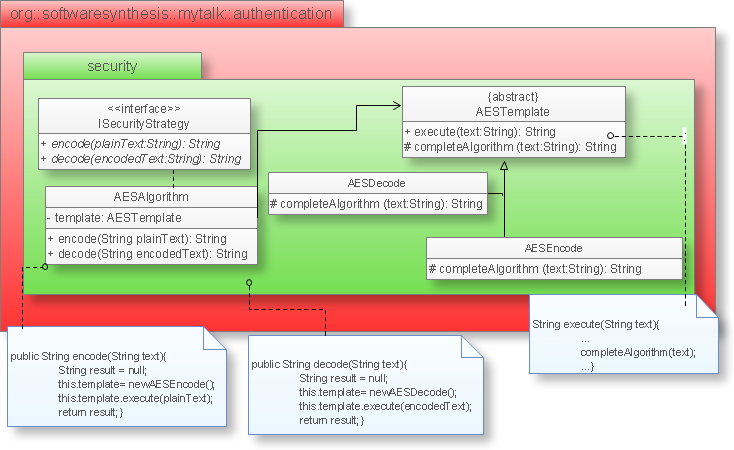
\includegraphics[width=\textwidth]{DDPAuthenticationSecurity}
\caption{Diagramma package server.authentication.security}
\end{figure}
\end{center}

\classsection{ISecurityStrategy}

\subsubsection*{Funzione}
Interfaccia che identifica il comportamento di una strategia generica di crittografia dei dati.

\subsubsection*{Relazioni d'uso}
Nessuna relazione d'uso evidenziata.

\subsubsection*{Classi estese ed interfacce implementate}

Nessuna relazione d'uso evidenziata.

\subsubsection*{Metodi}
\begin{description}
	\item{\method{+ encrypt(plainText: String): String}}\\
	Cripta la stringa di testo ricevuta come parametro e la restituisce al chiamante.\\\\
	Il metodo può solleva eccezioni:
	\begin{itemize}
		\item \exception{IOException}: l'implementazione di tale metodo dovrà predisporre il lancio di un eccezione qualora il messaggio passato al metodo (plainText) sia vuoto.
	\end{itemize}
	\item{\method{+ decrypt(encryptedText: String)}}\\
	Decripta la stringa di testo ricevuta come parametro e la restituisce al chiamante.\\\\
	Il metodo può sollevare eccezioni:
	\begin{itemize}
		\item \exception{IOException}: l'implementazione di tale metodo dovrà predisporre il lancio di un eccezione qualora il messaggio passato al metodo (plainText) sia vuoto.
	\end{itemize}
\end{description}

\classsection{AESAlgorithm}

\subsubsection*{Funzione}
Implementazione della strategia di codifica/decodifica con l'uso dell'algoritmo AES a 128bit.

\subsubsection*{Relazioni d'uso}
\begin{itemize}
	\item \texttt{java.security.Key}: usata per creare un istanza di una chiave durante il processo di criptazione.
	\item \texttt{javax.crypto.Cipher}: usata per creare un istanza di un oggetto di criptazione che implementa l'algoritmo AES a 128 bit.
	\item \texttt{javax.crypto.spec.SecretKeySpec}: usata dall'algoritmo di per costruire una chiave segreta a partire da un array di byte.
	\item \texttt{sun.misc.BASE64Encoder}: utilizzata per eseguire una trasformazione da stringa a byte.
	\item \texttt{sun.misc.BASE64Decoder}: utilizzata per eseguire una trasformazione da byte in stringa.
\end{itemize}

\subsubsection*{Classi estese ed interfacce implementate}
\begin{itemize}
	\item \classname{ISecurityStrategy}: interfaccia d'implementazione.
\end{itemize}

\subsubsection*{Attributi}
\begin{description}
  \item{\memberdata{-- \{frozen\} \underline{keyValue}: byte[]}}\\
  Array di byte usato per definire il valore della chiave su cui si basa l'algoritmo AES di criptazione. La chiave effettiva sarà creata a partire da tale attributo, per mezzo della classe \texttt{javax.crypto.spec.SecretKeySpec}.
  \item{\memberdata{-- \{frozen\} \underline{algorithm}: String}}\\
  Stringa costante che identifica il nominativo dell'algoritmo usato, e che dovrà essere specificato durante l'uso di \texttt{javax.crypto.Cipher}. l'attributo avrà valore ``AES''.
\end{description}

\subsubsection*{Metodi}
\begin{description}
	\item{\method{- generateKey(): Key}}\\
	Metodo che restituisce una chiave di tipo \texttt{java.security.Key}, a partire dall'array \memberdata{keyValue}. Per fare ciò, il metodo usa il costruttore di \texttt{javax.crypto.spec.SecretKeySpec}.
	Il metodo può sollevare eccezioni:
	\begin{itemize}
		\item \exception{Exception}: il metodo può sollevare un'eccezione generica.
	\end{itemize}
	\item{\method{+ encrypt(plainText: String): String}}\\
	Metodo usato per criptare un testo di tipo \texttt{String} passato come parametro d'ingresso. Il metodo usa una chiave ottenuta a partire dal metodo \method{generateKey()} in associazione alla classe \texttt{javax.crypto.Cipher} per criptare il testo tramite l'algoritmo AES.
	\begin{itemize}
		\item \exception{Exception}: il metodo solleva un'eccezione.
	\end{itemize}
	\item{\method{+ decrypt(encryptedText: String)}}\\
	Decripta la stringa di testo ricevuta come parametro, attuando una procedura inversa a quella presentata nel metodo \method{encrypt(plainText: String)}\\\\
	Il metodo può sollevare eccezioni:
	\begin{itemize}
		\item \exception{Exception}: il metodo può sollevare un'eccezione generica.
	\end{itemize}
\end{description}

\classsection{AESTemplate}

\subsubsection*{Funzione}
Rappresenta la struttura dell'algoritmo di crittografia AES a 128 bit, implementa inoltre \texttt{template method}.

\subsubsection*{Relazioni d'uso}
\begin{itemize}
	\item \texttt{java.security.Key};
	\item \texttt{javax.crypto.Cipher};
	\item \texttt{javax.crypto.spec.SecretKeySpec};
\end{itemize}

\subsubsection*{Classi estese ed interfacce implementate}

Nessuna relazione evidenziata.

\subsubsection*{Attributi}
\begin{description}
  \item{\memberdata{-- key: byte[]}}\\
  Array di byte usato per definire il valore della chiave su cui si basa l'algoritmo AES di criptazione. La chiave effettiva sarà creata a partire da tale attributo per mezzo della classe \texttt{javax.crypto.spec.SecretKeySpec}.
  \item{\memberdata{-- cipher: Cipher}}\\
  Oggetto rappresentante l'algoritmo di criptazione.
  \item{\memberdata{-- generated: Key}}\\
  Oggetto rappresentante la chiave generata dall'algoritmo di criptazione.
\end{description}

\subsubsection*{Metodi}
\begin{description}

	\item{\method{+ AESTemplate()}}\\
	Costruttore pubblico. imposta key con il seguente contenuto:\\
	\verb|new byte[]{'C', 'p', '2', 'Q', 'j', 'w', 'M', 'F', '7', 'e', 'j', 'N', 't', 'd', 'b', '1'};|.

	\item{\method{+ \{frozen\} execute(text: String): String}}\\
	Metodo che definisce l'iter di esecuzione di una generica procedura riguardante il sistema di sicurezza. Il metodo si occupa di inizializzare il cifratore \memberdata{cipher} mediante il metodo \texttt{getIstance(''AES'')}, quindi si imposta il contenuto di \memberdata{generated} con ciò che viene restituito da \texttt{SecretKeySpec(this.key, ''AES'')}. Il metodo invoca \method{compleateAlgorithm}, e salva il suo valore di ritorno in una Stringa denominata \texttt{result}, terminando restituendo \texttt{result}.

	\item{\method{\# \{abstract\} compleateAlgotihm(text: String): String}}\\
	Metodo astratto. Costituisce l'implementazione del pattern \texttt{template method}.

	\item{\method{\# getCipher(): Cipher}}\\
	Metodo che restituisce il cifratore \memberdata{cipher} alle sottoclassi in modo che possano criptare/decriptare il testo.

	\item{\method{\# getGenerateKey(): Key}}\\
	Metodo che restituisce una chiave di tipo \texttt{java.security.Key}, a partire dall'attributo \memberdata{generated}.
	
\end{description}

\classsection{AESEncode}

\subsubsection*{Funzione}
Rappresenta la struttura dell'algoritmo di criptazione usato nel sistema, ridefinisce il metodo astratto \method{compleateAlgorithm} della classe padre \classname{AESTemplate}.

\subsubsection*{Relazioni d'uso}
\begin{itemize}
	\item \texttt{javax.crypto.Cipher}: usato come cifratore durante la procedura di criptazione;
	\item \texttt{sun.misc.BASE64Encoder}: encoder di criptazione.
\end{itemize}

\subsubsection*{Classi estese ed interfacce implementate}

\begin{itemize}
	\item \classname{AESTemplate}: classe estesa.
\end{itemize}

\subsubsection*{Attributi}

Nessun attributo evidenziato.

\subsubsection*{Metodi}
\begin{description}

	\item{\method{\# \{final\} compleateAlgotihm(text: String): String}}\\
	Metodo usato per definire l'algoritmo di criptazione, esso definisce un oggetto di tipo \texttt{BASE64Encoder} denominato encoder e lo inizializza con il suo costruttore di default. Quindi si definisce un array di byte (buffer) in cui si dovrà caricare il contenuto del testo da criptare. Si osservi che per tale operazione è richiesto l'utilizzo del metodo \texttt{getBytes()} eseguito a partire da \textit{text}. Quindi il metodo prosegue definendo  un cifratore di tipo \texttt{Cipher}. Una stringa \texttt{result} sarà usata per restituire il risultato dell'operazione di criptazione. Il prossimo passaggio definisce il cuore della procedura di criptazione, ed è importante che lo sviluppatore si attenga scrupolosamente a quanto qui riportato. Il metodo definisce le istruzioni:\\
	
	\verb|cipher.init(Cipher.ENCRYPT_MODE, super.getGeneratedKey());|\\
	\verb|buffer = cipher.doFinal(buffer);|\\
	\verb|result = encoder.encode(buffer);|\\
	
	Il metodo termina ritornando il contenuto di result.
	
\end{description}

\classsection{AESDecode}

\subsubsection*{Funzione}
Rappresenta la struttura dell'algoritmo di criptazione usato nel sistema, esso ridefinisce il metodo astratto \method{compleateAlgorithm} della classe padre \classname{AESTemplate}.

\subsubsection*{Relazioni d'uso}
\begin{itemize}
	\item \texttt{javax.crypto.Cipher}: usato come cifratore durante la procedura di decriptazione;
	\item \texttt{sun.misc.BASE64Decoder}: decoder di decriptazione.
\end{itemize}

\subsubsection*{Classi estese ed interfacce implementate}

\begin{itemize}
	\item \classname{AESTemplate}: classe estesa.
\end{itemize}

\subsubsection*{Attributi}

Nessun attributo evidenziato.

\subsubsection*{Metodi}
\begin{description}

	\item{\method{\# \{final\} compleateAlgotihm(text: String): String}}\\
	Metodo usato per definire l'algoritmo di decriptazione, esso definisce un oggetto di tipo \texttt{BASE64Decoder} denominato decoder e lo inizializza con il suo costruttore di default. Quindi si definisce un array di byte (buffer) in cui si dovrà caricare il contenuto del testo da decriptare. Si osservi che per tale operazione è richiesto l'utilizzo del metodo \texttt{decodeBuffer(text)} eseguito a partire da decoder. Quindi il metodo prosegue definendo  un cifratore di tipo \texttt{Cipher}. Una stringa \texttt{result} sarà usata per restituire il risultato dell'operazione . Il prossimo passaggio definisce il cuore della procedura di decriptazione, ed è importante che lo sviluppatore si attenga scrupolosamente a quanto qui riportato. Il metodo definisce le istruzioni:\\
	
	\verb|cipher.init(Cipher.DECRYPT_MODE, super.getGeneratedKey());|\\
	\verb|buffer = cipher.doFinal(buffer);|\\
	\verb|result = new String(buffer);|\\
	
	Il metodo termina ritornando il contenuto di result.
	
\end{description}

\subsection{Package \texttt{org.softwaresynthesis.mytalk.server.authentication}}\label{sec:authentication}

\begin{center}
\begin{figure}[H]
  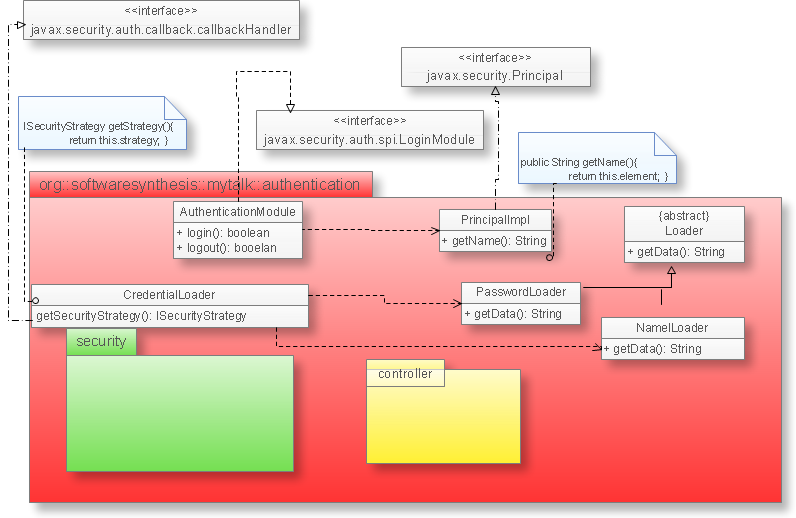
\includegraphics[width=\textwidth]{DDPAuthentication}
\caption{Diagramma package server.authentication}
\end{figure}
\end{center}

\classsection{PrincipalImpl}

\subsubsection*{Funzione}
Oggetto che permette di identificate univocamente uno \texttt{IUserData} memorizzato nel database del sistema \caName.

\subsubsection*{Relazioni d'uso}
\begin{itemize}
	\item \texttt{java.io.Serializable}: interfaccia d'implementazione usata per rendere serializzabili le istanze della classe.
	\item \texttt{java.security.Principal}: interfaccia d'implementazione usata per rendere caratterizzate le istanze della classe.
\end{itemize}

\subsubsection*{Classi estese ed interfacce implementate}

Nessuna relazione evidenziata.

\subsubsection*{Attributi}
\begin{description}
  \item{\memberdata{-- \{frozen\} \underline{serialVersionUID}: long}}\\
  Identificativo univoco per la classe, usato al fine di rendere l'oggetto serializzabile.
  \item{\memberdata{-- mail: String}}\\
  Attributo che rappresenta l'indirizzo e-mail dell'utente.
\end{description}

\subsubsection*{Metodi}
\begin{description}
	\item{\method{+ PrincipalImpl(mail: String)}}\\
	Classe costruttore. crea un oggetto \texttt{PrincipalImpl} che permette di determinare univocamente lo \texttt{IUserData} che ha effettuato il login.
	\item{\method{+ getName(): String}}\\
	Restituisce l'elemento identificativo (mail dell'utente) dello \texttt{IUserData} che ha effettuato la procedura di login.
	\item{\method{+ equals(obj: Object): boolean}}\\
	Verifica l'uguaglianza di due oggetti \texttt{PrincipalImpl} sulla base di un confronto tra gli indirizzi mail degli utenti confrontati.
	\item{\method{+ hashCode(): int}}\\
	Restituisce il codice \textit{hash} dell'oggetto di invocazione.				\item{\method{+ toString(): String}}\\
	Restituisce l'istanza dell'oggetto sotto forma di stringa. In particolare evidenziando l'indirizzo e-mail dell'utente.
\end{description}

\classsection{AuthenticationModule}

\subsubsection*{Funzione}
Modulo di autenticazione utilizzato dal sistema \caName.

\subsubsection*{Relazioni d'uso}
\begin{itemize}
	\item \texttt{java.io.IOException}: la classe è in grado di sollevare eccezioni relative a operazioni di IO.
	\item \texttt{java.security.Principal}: interfaccia che definisce i dati di autenticazione di un utente.
	\item \texttt{java.util.Map}: parametri passati ad \method{inizialize()}.
	\item \texttt{java.util.Set}: la classe può definire istanze di \texttt{Set}, per memorizzare i dati trattati.
	\item \texttt{javax.security.auth.callback.Callback}: vettore utilizzato per contenere i dati di autenicazione.
	\item \texttt{javax.security.auth.callback.CallbackHandler}: parametri passati ad \method{inizialize()}.
	\item \texttt{javax.security.auth.callback.NameCallback}: oggetto che contiene il \texttt{name} dell'utente da autenticare.
	\item \texttt{javax.security.auth.callback.PasswordCallback}: oggetto che contiene la password dell'utente da autenticare.
	\item \texttt{javax.security.auth.callback.UnsupportedCallbackException}: la classe è in grado di sollevare eccezioni relative a operazioni di \texttt{UnsupportedCallback}.
	\item \texttt{javax.security.auth.login.FailedLoginException}: la classe è in grado di sollevare eccezioni relative a operazioni di \texttt{FailedLoginException}.
	\item \texttt{javax.security.auth.login.LoginException}: la classe è in grado di sollevare eccezioni relative a operazioni di \texttt{LoginException}.
	\item \texttt{javax.security.auth.Subject}: definisce il soggetto da autenticare.
	\item \classname{abook.IUserData}: la classe interagisce con istanze di oggetti identificabili come utenti.
	\item \classname{dao.UserDataDAO}: utilizzata per modificare il contenuto del database. Nello specifico viene usata per interagire con la tabella \texttt{UserData}.
\end{itemize}

\subsubsection*{Classi estese ed interfacce implementate}
\begin{itemize}
	\item \texttt{javax.security.auth.spi.LoginModule}: interfaccia d'implementazione.
\end{itemize}

\subsubsection*{Attributi}
\begin{description}
  \item{\memberdata{-- login: boolean}}\\
  Attributo che determina se il login è avvenuto oppure no.
  \item{\memberdata{-- commit: boolean}}\\
  Attributo che determina se il commit è già stato eseguito.
  \item{\memberdata{-- handler: CallbackHandler}}\\
  Oggetto utilizzato per il caricamento delle credenzialie.
  \item{\memberdata{-- password: char[]}}\\
  Attributo che che contiene la \textit{password} immessa dall'utente.
  \item{\memberdata{-- username: String}}\\
   Attributo che che contiene lo \textit{username} immesso dall'utente.
  \item{\memberdata{-- principal: Principal}}\\
  Contiene la caratteristica autenticativa del subject. Nel sistema MyTalk tale proprietà è riservata al campo mail.
  \item{\memberdata{-- subject: Subject}}\\
  Attributo che definisce il soggetto da autenticare.
\end{description}

\subsubsection*{Metodi}
\begin{description}
	\item{\method{+ initialize(subject: Subject, handler: CallbackHandler, sharedState: Map, option: Map): void }}\\
	Il metodo ha il compito di inizializzare gli attributi privati della classe con i parametri d'input.

	\item{\method{+ login(): boolean throws LoginException}}\\
	Metodo richiamato per verificare un riscontro tra i dati passati per l'autenticazione e i dati presenti nel database. Il metodo deve appoggiarsi alla classe \classname{UserDataDAO} per le operazione di estrazione dati dal database.
	
	\item{\method{+ commit(): boolean throws LoginException}}\\
	Metodo richiamato direttamente dal framework se il login va a buon fine. Il suo scopo è quellodi inizializzare il \textit{subject} con i relativi \textit{principle}.
	
	\item{\method{+ abort(): boolean throws LoginException}}\\
	Metodo usato per bloccare la procedura di login.
	
	\item{\method{+ logout(): boolean throws LoginException}}\\
	Metodo per il logout del sistema. Il suo scopo è quello di eliminare il \textit{principle} e il \textit{subject}.

\end{description}

\classsection{CredentialLoader}

\subsubsection*{Funzione}
Permette di caricare le credenziali di autenticazione, fornite dall'utente, per preparare la fase di login.

\subsubsection*{Relazioni d'uso}
\begin{itemize}
	\item \texttt{javax.security.auth.callback.Callback}: usato durante la procedura di inserimento dati.
	\item \texttt{javax.security.auth.callback.NameCallback}: tipo di dato richiesto in ingresso per completare la parte di login.
	\item \texttt{javax.security.auth.callback.PasswordCallback}: tipo di dato richiesto in ingresso per completare la parte di login.
	\item \texttt{java.io.IOException}: eccezione che può essere sollevata dal metodo \texttt{handle} definito dall'interfaccia \texttt{javax.security.auth.callback.CallbackHandler}.
	\item \texttt{javax.security.auth.callback.UnsupportedCallbackException}: eccezione che può essere sollevata dal metodo \texttt{handle} definito dall'interfaccia \texttt{javax.security.auth.callback.CallbackHandler}.
\end{itemize}

\subsubsection*{Classi estese ed interfacce implementate}
\begin{itemize}
	\item \texttt{javax.security.auth.callback.CallbackHandler}: Interfaccia implementata dalla classe.
\end{itemize}

\subsubsection*{Attributi}
\begin{description}
  \item{\memberdata{-- credential: AuthenticationData}}\\
  Attributo contenente i dati da autenticare per la login dell'utente.
  \item{\memberdata{-- security: ISecurityStrategy}}\\
  Attributo che contiene un oggetto che definisce un algoritmo di criptazione per i dati. Necessario per criptare i dati di autenticazione.
\end{description}

\subsubsection*{Metodi}
\begin{description}
	\item{\method{+ CredentialLoader(credential: AuthenticationData, security: ISecurityStrategy)}}\\
	Costruttore pubblico. Crea un istanza con le credenziali fornite dall'utente (fornite in fase di login).

	\item{\method{+ handle(callbacks: Callback[]): void}}\\
	Effettua il caricamento e crittografa delle credenziali fornite dall'utente per la fase di login\\\\
	Il metodo può sollevare eccezioni:
	\begin{itemize}
		\item \exception{IOException}
		\item \exception{UnsupportedCallbackException}
	\end{itemize}

\end{description}

\classsection{Loader}

\subsubsection*{Funzione}
Oggetto usato per il caricamento delle credenziali di autenticazione.

\subsubsection*{Relazioni d'uso}
\begin{itemize}
	\item \texttt{java.io.IOException};
	\item \texttt{javax.servlet.http.HttpServletRequest};
	\item \texttt{org.softwaresynthesis.mytalk.server.authentication.security.ISecurityStrategy}: usata per definire l'algoritmo di criptazione.
\end{itemize}

\subsubsection*{Classi estese ed interfacce implementate}

\begin{itemize}
	\item \texttt{javax.security.auth.callback.Callback}: interfaccia d'implementazione.
\end{itemize}

\subsubsection*{Attributi}
\begin{description}
  \item{\memberdata{-- callback: Callback}}\\
  \item{\memberdata{-- strategy: ISecurityStrategy}}\\
\end{description}

\subsubsection*{Metodi}
\begin{description}
	\item{\method{+ Loader(callback: Callback)}}\\
	Costruttore pubblico. Crea il ''caricatore'' con la giusta istanza di \texttt{callback}.
	
	\item{\method{\# getCallback(): callback}}\\
	Metodo usato per ritornare l'attributo \memberdata{callback}.
	
	\item{\method{\# getISecurityStrategy(): ISecurityStrategy}}\\
	Metodo usato per ritornare l'attributo \memberdata{strategy}.
	
\end{description}

\classsection{NameLoader}

\subsubsection*{Funzione}
Caricatore per lo \textit{username}. Ha il compito di caricare e preparare lo \textit{username} fornito dall'utente per la successiva fase di autenticazione.

\subsubsection*{Relazioni d'uso}
\begin{itemize}
	\item \texttt{java.io.IOException};
	\item \texttt{javax.servlet.http.HttpServletRequest};
	\item \texttt{javax.security.auth.callback.NameCallback)};
\end{itemize}

\subsubsection*{Classi estese ed interfacce implementate}

\begin{itemize}
	\item \texttt{Loader}: classe estesa.
\end{itemize}

\subsubsection*{Attributi}

Nessun attributo evidenziato.

\subsubsection*{Metodi}
\begin{description}
	\item{\method{+ NameLoader()}}\\
	Costruttore pubblico che richiama il costruttore della super classe passando come parametro: \verb|new NameCallback("username")|.
	
	\item{\method{+ load(request: HttpServletRequest): void}}\\
	Il metodo crea un istanza di \texttt{NameCallback} a partire dalla \textit{callback} ottenuta dalla chiamata \verb|super.getCallback()|. Quindi carica in una variabile locale di tipo \texttt{String} il nome dell'utente. Tale parametro si ottiene mediante una chiamata a metodo getParameter(''username'') invocata dall'istanza \textit{request}. Quindi si imposta tale nome sull'istanza callback (usare \verb|callback.setName(username)|).
	
	\item{\method{+ getData(): String}}\\
	Metodo usato per ottenere il nome dell'utente. Il metodo ritorna il contenuto di una chiamata \verb|super.getCallback().getName()|.
	
\end{description}

\classsection{PasswordLoader}

\subsubsection*{Funzione}
Caricatore per la \textit{password}. Ha il compito di caricare e preparare la \textit{password} fornita dall'utente per la successiva fase di autenticazione.

\subsubsection*{Relazioni d'uso}
\begin{itemize}
	\item \texttt{java.io.IOException};
	\item \texttt{javax.servlet.http.HttpServletRequest};
	\item \texttt{javax.security.auth.callback.PasswordCallback)};
\end{itemize}

\subsubsection*{Classi estese ed interfacce implementate}

\begin{itemize}
	\item \texttt{Loader}: classe estesa.
\end{itemize}

\subsubsection*{Attributi}

Nessun attributo evidenziato.

\subsubsection*{Metodi}
\begin{description}
	\item{\method{+ PasswordLoader()}}\\
	Costruttore pubblico che richiama il costruttore della super classe passando come parametro: \verb|new PasswordCallback("password")|.
	
	\item{\method{+ load(request: HttpServletRequest): void}}\\
	Il metodo crea un istanza di \texttt{PasswordCallback} a partire dalla \textit{callback} ottenuta dalla chiamata \verb|super.getCallback()|. Quindi carica in una variabile locale di tipo \texttt{String} la \textit{password} dell'utente, ed usando l'algoritmo di sicurezza definito dall'istanza di tipo ISecurityStrategy, cripta la \textit{password}. Tale parametro si ottiene mediante una chiamata a metodo getParameter(''password'') invocata dall'istanza \textit{request}. Quindi si imposta tale nome sull'istanza \textit{callback} (usare \verb|callback.setName(PASSWORD_CRIPTATA)|).
	
	\item{\method{+ getData(): String}}\\
	Metodo usato per ottenere la \textit{password} dell'utente. Il metodo salva il contenuto di una chiamata \verb|super.getCallback().getPassword()|. Poi, prima di ritornare il valore, esegue la decriptazione mediante l'algoritmo \texttt{ISecurityStrategy} utilizzato.
	
\end{description}

\subsection{Package \texttt{org.softwaresynthesis.mytalk.server.authentication.controller}}\label{sec:autservlet}

\begin{center}
\begin{figure}[H]
  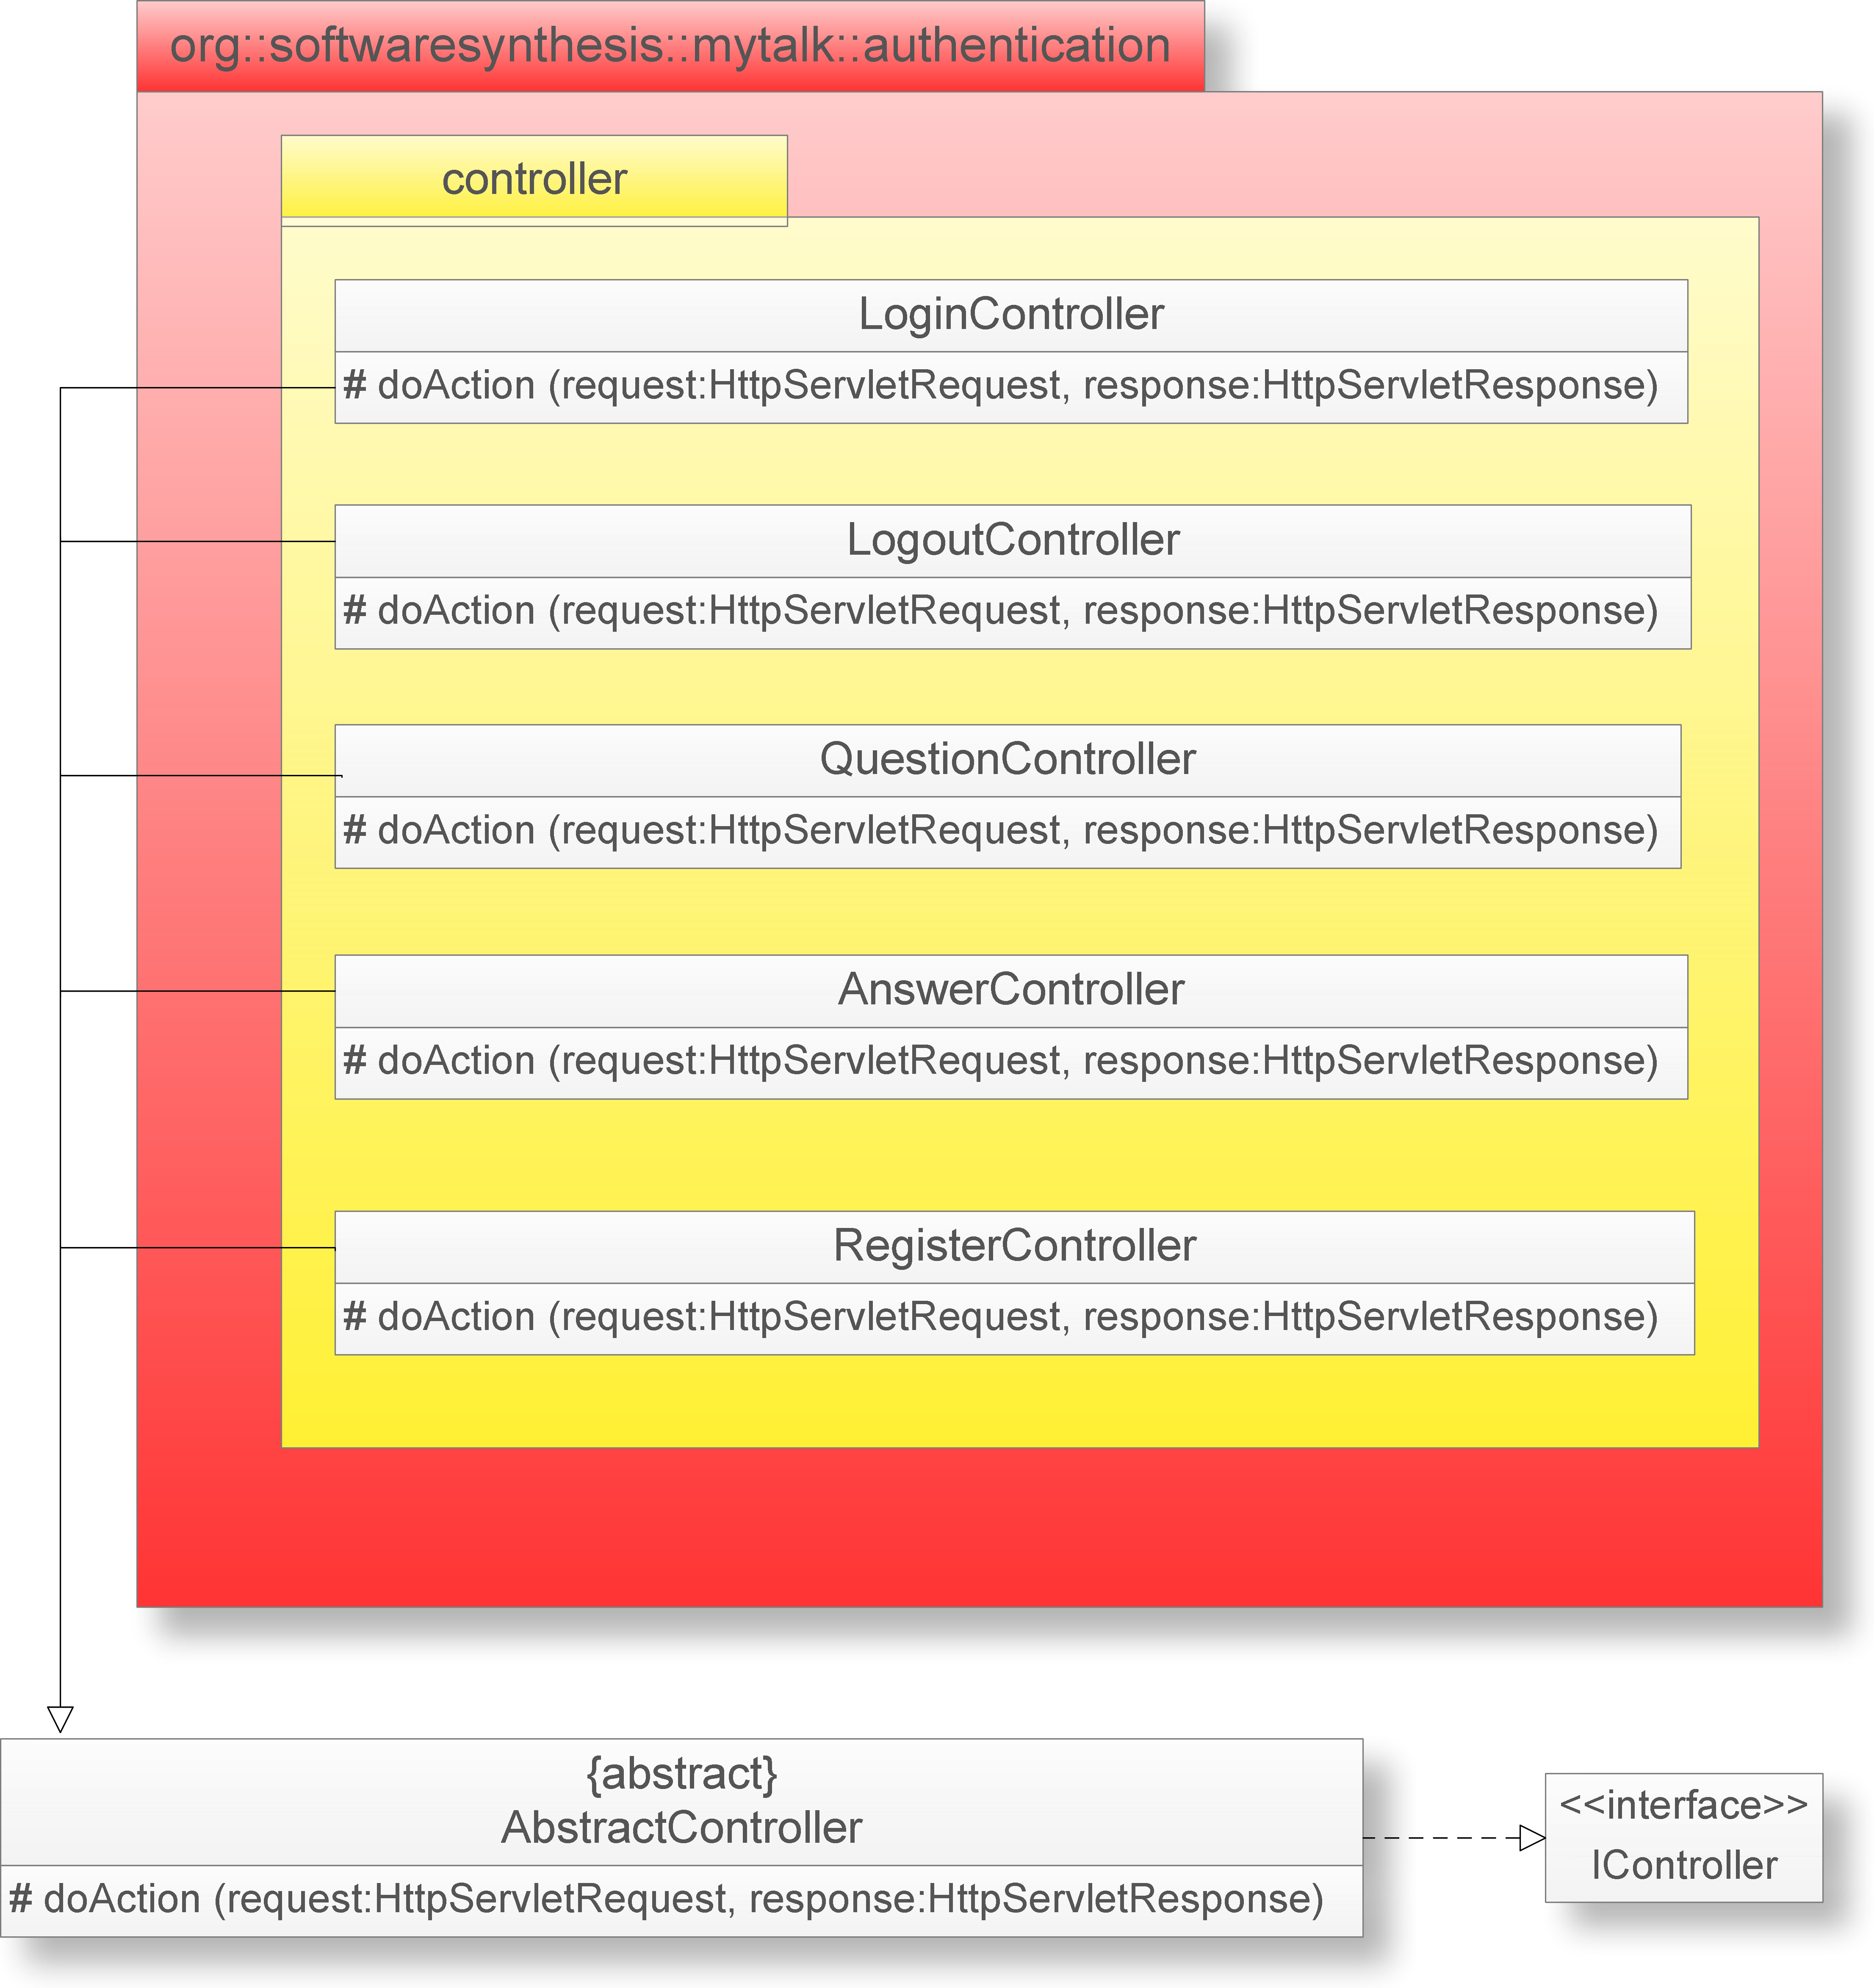
\includegraphics[width=\textwidth]{DDPAuthenticationController}
\caption{Diagramma package server.authentication.controller}
\end{figure}
\end{center}

%TODO da rivedere nella definizione dei metodi! 
\classsection{LogoutController}

\subsubsection*{Funzione}
\inglese{Controller} da richiamare per effettuare il logout dal sistema.

\subsubsection*{Relazioni d'uso}
\begin{itemize}
	\item \texttt{java.io.IOException}: eccezione richiamabile dal metodo\method{doAction()}.
	\item \texttt{java.io.PrintWriter}: classe istanziata all'interno del metodo \method{doAction()}. Usata per scrivere l'output della \inglese{servlet}.
	\item \texttt{javax.servlet.ServletException}: eccezione sollevabile dai metodi \method{doAction()}.
	\item \texttt{javax.servlet.http.HttpServletRequest}: classe usata per interagire con le richieste AJAX inoltrate dal client.
	\item \texttt{javax.servlet.http.HttpServletResponse}: classe usata per interagire con le richieste AJAX inoltrate dal client.
	\item \classname{abook.IUserData}: usata per definire un utente.
	\item \classname{dao.DataPersistanceManager}: usata per comunicare tramite Hibernate con la tabella \texttt{UserData} della base di dati.
\end{itemize}

\subsubsection*{Classi estese ed interfacce implementate}
\begin{itemize}
	\item \texttt{server.AbstractController}: classe estesa.
\end{itemize}

\subsubsection*{Attributi}

Nessun attributo evidenziato

\subsubsection*{Metodi}
\begin{description}
	\item{\method{\# doAction(request: HttpServletRequest, response: HttpServletResponse): void}}\\
	Metodo che costituisce il kernel logico di risposta del \inglese{controller}. Il metodo inizia caricando i parametri ricevuti mediante \texttt{HttpServletRequest}. Una chiamata a tale \inglese{controller} corrisponde ad una richiesta di logout e si attua impostando a false la sessione contenuta nell'oggetto \texttt{HttpServletRequest request}. Il metodo procede con la creazione di un istanza  di \texttt{LoginContext} denominata \texttt{context}. Quindi viene effettuata la memorizzazione dell'oggetto ritornato da una chiamata:
\\
\verb|session.getAttribute("LoginContext");|
\\

L'oggetto cosi ottenuto dovrà essere controllato, ovvero si dovrà accertare che il tipo dinamico è conforme al tipo \texttt{LoginContext} (il programmatore dovrà obbligatoriamente usare   la primitiva \texttt{istanceof}). Quindi si sovrascrive il contenuto di \texttt{context} con quanto ottenuto dalla chiamata a metodo sopracitata, e si richiama il metodo \texttt{logout()} a partire dall'oggetto \texttt{context}. Il metodo termina invalidando la sessione richiamando il metodo \texttt{invalidate()} di \texttt{HttpSession}.

\end{description}

\classsection{LoginController}

\subsubsection*{Funzione}
\inglese{Controller} da richiamare per effettuare l'autenticazione dell'utente.

\subsubsection*{Relazioni d'uso}
\begin{itemize}
\item \texttt{java.io.IOException}: eccezione richiamabile dal metodo\method{doAction()}.
	\item \texttt{java.io.PrintWriter}: classe istanziata all'interno del metodo \method{doAction()}. Usata per scrivere l'output della \inglese{servlet}.
	\item \texttt{javax.servlet.ServletException}: eccezione sollevabile dai metodi \method{doAction()}.
	\item \texttt{javax.servlet.http.HttpServletRequest}: classe usata per interagire con le richieste AJAX inoltrate dal client.
	\item \texttt{javax.servlet.http.HttpServletResponse}: classe usata per interagire con le richieste AJAX inoltrate dal client.
	\item \classname{abook.IUserData}: usata per definire un utente.
	\item \classname{dao.DataPersistanceManager}: usata per comunicare tramite Hibernate con la tabella \texttt{UserData} della base di dati.
\end{itemize}

\subsubsection*{Classi estese ed interfacce implementate}
\begin{itemize}
	\item \texttt{server.AbstractController}: classe estesa.
\end{itemize}

\subsubsection*{Attributi}

Nessun attributo evidenziato

\subsubsection*{Metodi}
\begin{description}
	\item{\method{\# doAction(request: HttpServletRequest, response: HttpServletResponse): void}}\\

Il metodo inizia caricando i parametri ricevuti mediante \texttt{HttpServletRequest}. Una chiamata a tale metodo corrisponde ad una richiesta di login e si attua impostando due campi \texttt{String} con i dati ottenuti da una chiamata a \texttt{getParameter(``username'')} e \texttt{getParameter(``password'')}. Il metodo prosegue controllando se l'\textit{username} e la \textit{password} precedentemente ottenute hanno valore diverso da \texttt{null}. Nel caso il flusso principale continua creando un'istanza di \classname{AutenthicationData} (denominata \texttt{credential}) a partire dai parametri \textit{username} e \textit{password}. Quindi si carica la path del file di configurazione in un apposita stringa \texttt{pathFileConfig}, tramite la chiamata a metodo:\\
	
\verb|System.getenv("MyTalkConfiguration") + "\\LoginConfiguration.conf"|.\\

Il flusso principale prosegue all'interno di un blocco \texttt{try-catch} creando:
	\begin{itemize}
		\item[•] un \classname{CredentialLoader} (loader);
		\item[•] un \classname{LoginContext} (context);
		\item[•] un \classname{dao.UserDataDao} (user);
	\end{itemize}
Quindi tramite context si esegue il login e si impostano gli attributi di sessione come segue: 

\texttt{session.setAttribute("LoginContext", context);}

Infine si carica in user un istanza di \classname{dao.DataPersistanceManager} ottenuta dalla chiamata a metodo \method{DataPersistanceManager.getUserData()}, e restituendo user in un formato di formattazione \texttt{Json} (\texttt{user.toJson()}).

\end{description}

\classsection{RegisterController}

\subsubsection*{Funzione}
\inglese{Conroller} da richiamare per effettuare la registrazione al sistema MyTalk.

\subsubsection*{Relazioni d'uso}
\begin{itemize}
	\item \texttt{java.io.IOException}: eccezione richiamabile dal metodo\method{doAction()}.
	\item \texttt{java.io.PrintWriter}: classe istanziata all'interno del metodo \method{doAction()}. Usata per scrivere l'output della \inglese{servlet}.
	\item \texttt{javax.servlet.ServletException}: eccezione sollevabile dai metodi \method{doAction()}.
	\item \texttt{javax.servlet.http.HttpServletRequest}: classe usata per interagire con le richieste AJAX inoltrate dal client.
	\item \texttt{javax.servlet.http.HttpServletResponse}: classe usata per interagire con le richieste AJAX inoltrate dal client.
	\item \classname{abook.IUserData}: usata per definire un utente.
	\item \classname{dao.DataPersistanceManager}: usata per comunicare tramite Hibernate con la tabella \texttt{UserData} della base di dati.
	\item \classname{authentication.security.ISecurityStrategy}: usata per criptare/decriptare i dati da inviare/ricevere
	\item \classname{authentication.security.AESAlgorithm}: implementazione di \classname{authentication.ISecurityStrategy} usata dalla classe descritta.
	
\end{itemize}

\subsubsection*{Classi estese ed interfacce implementate}
\begin{itemize}
	\item \texttt{server.AbstractController}: classe estesa.
\end{itemize}

\subsubsection*{Attributi}

Nessun attributo evidenziato

\subsubsection*{Metodi}
\begin{description}
	\item{\method{\# doAction(request: HttpServletRequest, response: HttpServletResponse): void}}\\

Il metodo inizia caricando i parametri ricevuti mediante \texttt{HttpServletRequest}. Una chiamata a tale metodo corrisponde ad una richiesta di registrazione al sistema e si attua impostando i dati di registrazione:
	\begin{itemize}
		\item name;
		\item username;
		\item mail;
		\item password;
		\item path immagine;
		\item domanda segreta;
		\item risposta alla domanda segreta;
	\end{itemize}
	Per eseguire tali operazioni, il metodo predispone delle opportune variabili di tipo \texttt{String} e crea uno \classname{abook.IUserData} user. Quindi all'interno di un blocco \textit{try-catch} viene impostata una strategia di criptaggio dei dati (creando un istanza di \classname{authentication.security.AESAlgorithm}). Quindi vengono caricati i dati di registrazione nelle variabili precedentemente create. Per eseguire tali operazioni è necessario usare l'istruzione:\\
	
	\verb|request.getParameter("NOME_PARAMTERO")|\\
	
	dove i nomi dei parametri sono:
	\begin{itemize}
		\item username (usata per l'indirizzo mail);
		\item name;
		\item surname;
		\item password;
		\item answer;
		\item question;
		\item picturePath;
	\end{itemize}
	Il passo successivo (sempre dentro il blocco try) consiste nel creare un istanza di \classname{dao.DataPersistanceManager} \texttt{userDAO}, e nell'eseguire un operazione di \texttt{userDAO} \method{insert()} passando come parametro user (l'utente precedentemente creato). Il blocco \textit{try} termina impostando \texttt{result} a \texttt{true}.
	
	Per quanto riguarda il blocco \textit{catch}, in esso viene impostato \texttt{result} a \texttt{false}.
	
	Il metodo termina scrivendo in un \texttt{PrintWriter} il valore di \texttt{result}.
\end{description}

\classsection{QuestionController}

\subsubsection*{Funzione}
\inglese{Conroller} da richiamare per gestire la visualizzazione della domanda segreta per il recupero della \textit{password}.

\subsubsection*{Relazioni d'uso}
\begin{itemize}
	\item \texttt{java.io.IOException}: eccezione richiamabile dal metodo\method{doAction()}.
	\item \texttt{java.io.PrintWriter}: classe istanziata all'interno del metodo \method{doAction()}. Usata per scrivere l'output della \inglese{servlet}.
	\item \texttt{javax.servlet.ServletException}: eccezione sollevabile dai metodi \method{doAction()}.
	\item \texttt{javax.servlet.http.HttpServletRequest}: classe usata per interagire con le richieste AJAX inoltrate dal client.
	\item \texttt{javax.servlet.http.HttpServletResponse}: classe usata per interagire con le richieste AJAX inoltrate dal client.
	\item \classname{abook.IUserData}: usata per definire un utente.
	\item \classname{dao.DataPersistanceManager}: usata per comunicare tramite Hibernate con la tabella \texttt{UserData} della base di dati.
	\item \classname{authentication.security.ISecurityStrategy}: usata per criptare/decriptare i dati da inviare/ricevere
	\item \classname{authentication.security.AESAlgorithm}: implementazione di \classname{authentication.ISecurityStrategy} usata dalla classe descritta.
	
\end{itemize}

\subsubsection*{Classi estese ed interfacce implementate}
\begin{itemize}
	\item \texttt{server.AbstractController}: classe estesa.
\end{itemize}

\subsubsection*{Attributi}

Nessun attributo evidenziato

\subsubsection*{Metodi}
\begin{description}
	\item{\method{\# doAction(request: HttpServletRequest, response: HttpServletResponse): void}}\\

Il metodo inizia creando un istanza di \classname{DataPersistanceManager} DAO. Quindi si caricano i parametri ricevuti mediante \texttt{HttpServletRequest} e si usano per la creazione di un \classname{IUserData}. Ciò significa che il metodo dovrà creare una stringa per memorizzare la mail e inizializzarla con una chiamata \texttt{getParameter(''username'')} da eseguire a partire dal parametro d'ingresso \texttt{request}. Successivamente si inizializza una variabile \classname{IUserData} denominata user (ciò avviene con un istruzione \verb|dao.getUserData(mail)|). Quindi si definisce una clausola condizionale \textit{if-else}. Il ramo \textit{if} è caratterizzato dalla condizione \texttt{user != null}. Nel caso il metodo definisce al suo interno le istruzioni per restituire la domanda segreta. Le operazioni qui sono:
\begin{itemize}
	\item si definisce uno \texttt{String question} e lo si inizializza con \verb|user.getQuestion()|;
	\item si definisce un \texttt{PrintWriter writer};
	\item si scrive nel \texttt{writer} la domanda \texttt{question}.
\end{itemize}

Nel caso la condizione dell'\textit{if} risulti falsa, il metodo definisce un ramo \textit{else} con le istruzioni necessaria per scrivere nel \texttt{writer} la stringa \texttt{null}.
\end{description}

\classsection{AnswerController}

\subsubsection*{Funzione}
\inglese{Conroller} che ha lo scopo di verificare la risposta alla domanda segreta per il recupero della \textit{password}.

\subsubsection*{Relazioni d'uso}
\begin{itemize}
	\item \texttt{java.io.IOException}: eccezione richiamabile dal metodo\method{doAction()}.
	\item \texttt{java.io.PrintWriter}: classe istanziata all'interno del metodo \method{doAction()}. Usata per scrivere l'output della \inglese{servlet}.
	\item \texttt{javax.servlet.ServletException}: eccezione sollevabile dai metodi \method{doAction()}.
	\item \texttt{javax.servlet.http.HttpServletRequest}: classe usata per interagire con le richieste AJAX inoltrate dal client.
	\item \texttt{javax.servlet.http.HttpServletResponse}: classe usata per interagire con le richieste AJAX inoltrate dal client.
	\item \classname{abook.IUserData}: usata per definire un utente.
	\item \classname{dao.DataPersistanceManager}: usata per comunicare tramite Hibernate con la tabella \texttt{UserData} della base di dati.
	\item \classname{authentication.security.ISecurityStrategy}: usata per criptare/decriptare i dati da inviare/ricevere
	\item \classname{authentication.security.AESAlgorithm}: implementazione di \classname{authentication.ISecurityStrategy} usata dalla classe descritta.
	
\end{itemize}

\subsubsection*{Classi estese ed interfacce implementate}
\begin{itemize}
	\item \texttt{server.AbstractController}: classe estesa.
\end{itemize}

\subsubsection*{Attributi}

Nessun attributo evidenziato

\subsubsection*{Metodi}
\begin{description}
	\item{\method{\# doAction(request: HttpServletRequest, response: HttpServletResponse): void}}\\

Il metodo inizia definendo i seguenti oggetti:

\begin{itemize}
	\item DataPersistanceManager dao: oggetto usato per l'inizializzazione di \classname{IUserData};
	\item ISecurityStrategy strategy = getSecurityStrategyFactory();
	\item String mail: da inizializzare con \verb|request.getParameter("username")|;
	\item String answer: da inizializzare con \verb|request.getParameter("answer")|;
	\item String result;
	\item String password;
	\item IUserData user: da inizializzare con \verb|dao.getUserData(mail)|;
	\item PrintWriter writer;
\end{itemize}

A questo punto il metodo definisce un costrutto condizionale \textit{if-else}. L'\textit{if} viene definito con la condizione \texttt{answer != null}. Nel caso il metodo procede definendo un blocco \textit{try-catch}. Nel blocco \textit{try}, si procede sovrascrivendo \texttt{answer} con la criptazione di \texttt{answer} stesso. Tale operazione necessita dell'uso di \texttt{strategy.encode(answer)}. Ora se \texttt{answer} è uguale alla risposta presente nell'oggetto \texttt{user}, allora si procede decriptando la \textit{password} (usare \texttt{strategy.decode(user.getPassword())}) e definendo la seguente istruzione:\\

\verb|boolean success = this.sendMail("mytalk@softwaresynthesis.org",|\\
\verb|user.getMail(), "Recupero password", password);|\\

Se \texttt{success} contiene il valore \texttt{true} allora il metodo imposta \texttt{result} a \texttt{true}, altrimenti lo imposta a \texttt{null}. Se in seguito al controllo precedente si osserva che \texttt{answer} è uguale a \texttt{null}, allora il metodo imposta \texttt{result} a \texttt{null}. Analogamente si fa nel ramo \textit{catch} del blocco \textit{try-catch} creato in precedenza. Il metodo termina scrivendo in \texttt{write} il risultato \texttt{result}.

\item{\method{+ sendMail(sender: String, receiver: String, subject: String, text: String): boolean}}\\

Il metodo viene usato per inviare una mail all'utente che sta cercando di autenticarsi presso il sistema. Tale procedura richiede obbligatoriamente l'impostazione di un host e di una porta. Lo sviluppatore dovrà usare le seguenti istruzioni:\\

\verb|String host = "smtp.gmail.com";|\\
\verb|int port = 465;|\\

Il metodo prosegue definendo un oggetto \classname{Properties} props.  Quindi si impostano le proprietà mediante le seguenti  istruzioni:\\

\verb|props.put("mail.smtp.auth", "true");|\\
\verb|props.put("mail.smtp.user", "MyTalk@softwaresynthesis.org");|\\
\verb|props.put("mail.smtp.host", host);|\\
\verb|props.put("mail.smtp.port", port);|\\
\verb|props.put("mail.smtp.starttls.enable","true");|\\
\verb|props.put("mail.smtp.socketFactory.port", port);|\\
\verb|props.put("mail.smtp.socketFactory.class", "javax.net.ssl.SSLSocketFactory");|\\
\verb|props.put("mail.smtp.socketFactory.fallback", "false");|\\

Quindi si definisce una sessione (\classname{Session}), e si procede con la creazione delle \texttt{''BodyParts''} del messaggio. Tale procedura avviene dentro ad un blocco try catch. Il metodo definisce tre blocchi di eccezioni catch:
\begin{itemize}
	\item catch(AddressException ae);
	\item catch(NoSuchProviderException nspe);
	\item catch(MessagingException me);
\end{itemize}

All'interno di questi blocchi viene eseguita un operazione di \texttt{return} \texttt{true}.

Il blocco \textit{try} invece procede come segue:

\begin{itemize}
	\item si costruisce un MimeMessage msg a partire dalla sessione precedentemente creata;
	\item si costruisce l'header del messaggio nel seguente modo:\\
	
		\verb|msg.setSubject("Recupero password");|\\
	    \verb|msg.setSentDate(new Date());|\\
	    \verb|msg.setFrom(new InternetAddress("MyTalk@softwaresynthesis.org"));|\\
	\item a partire dai parametri d'ingresso del metodo si definisce il ricevente receiver del messaggio e il corpo text;
	\item infine si impostano le procedure per l'invio della mail. Data la sensibilità di tale fase, è importante che il programmatore riporti l'utilizzo dell'oggetto \classname{Trasport} cosi come qui descritto:\\
	
		\verb|Transport transport = getTransport(session, "smtps");|\\
		\verb|transport.connect(host, "software.synthesis@gmail.com", "ingegneria");|\\
		\verb|transport.sendMessage(msg, msg.getAllRecipients());|\\
		\verb|transport.close();|
\end{itemize}

\end{description}

\subsection{Package \texttt{org.softwaresynthesis.mytalk.server.connection}}\label{sec:connection}

%\begin{center}
%\begin{figure}[H]
%  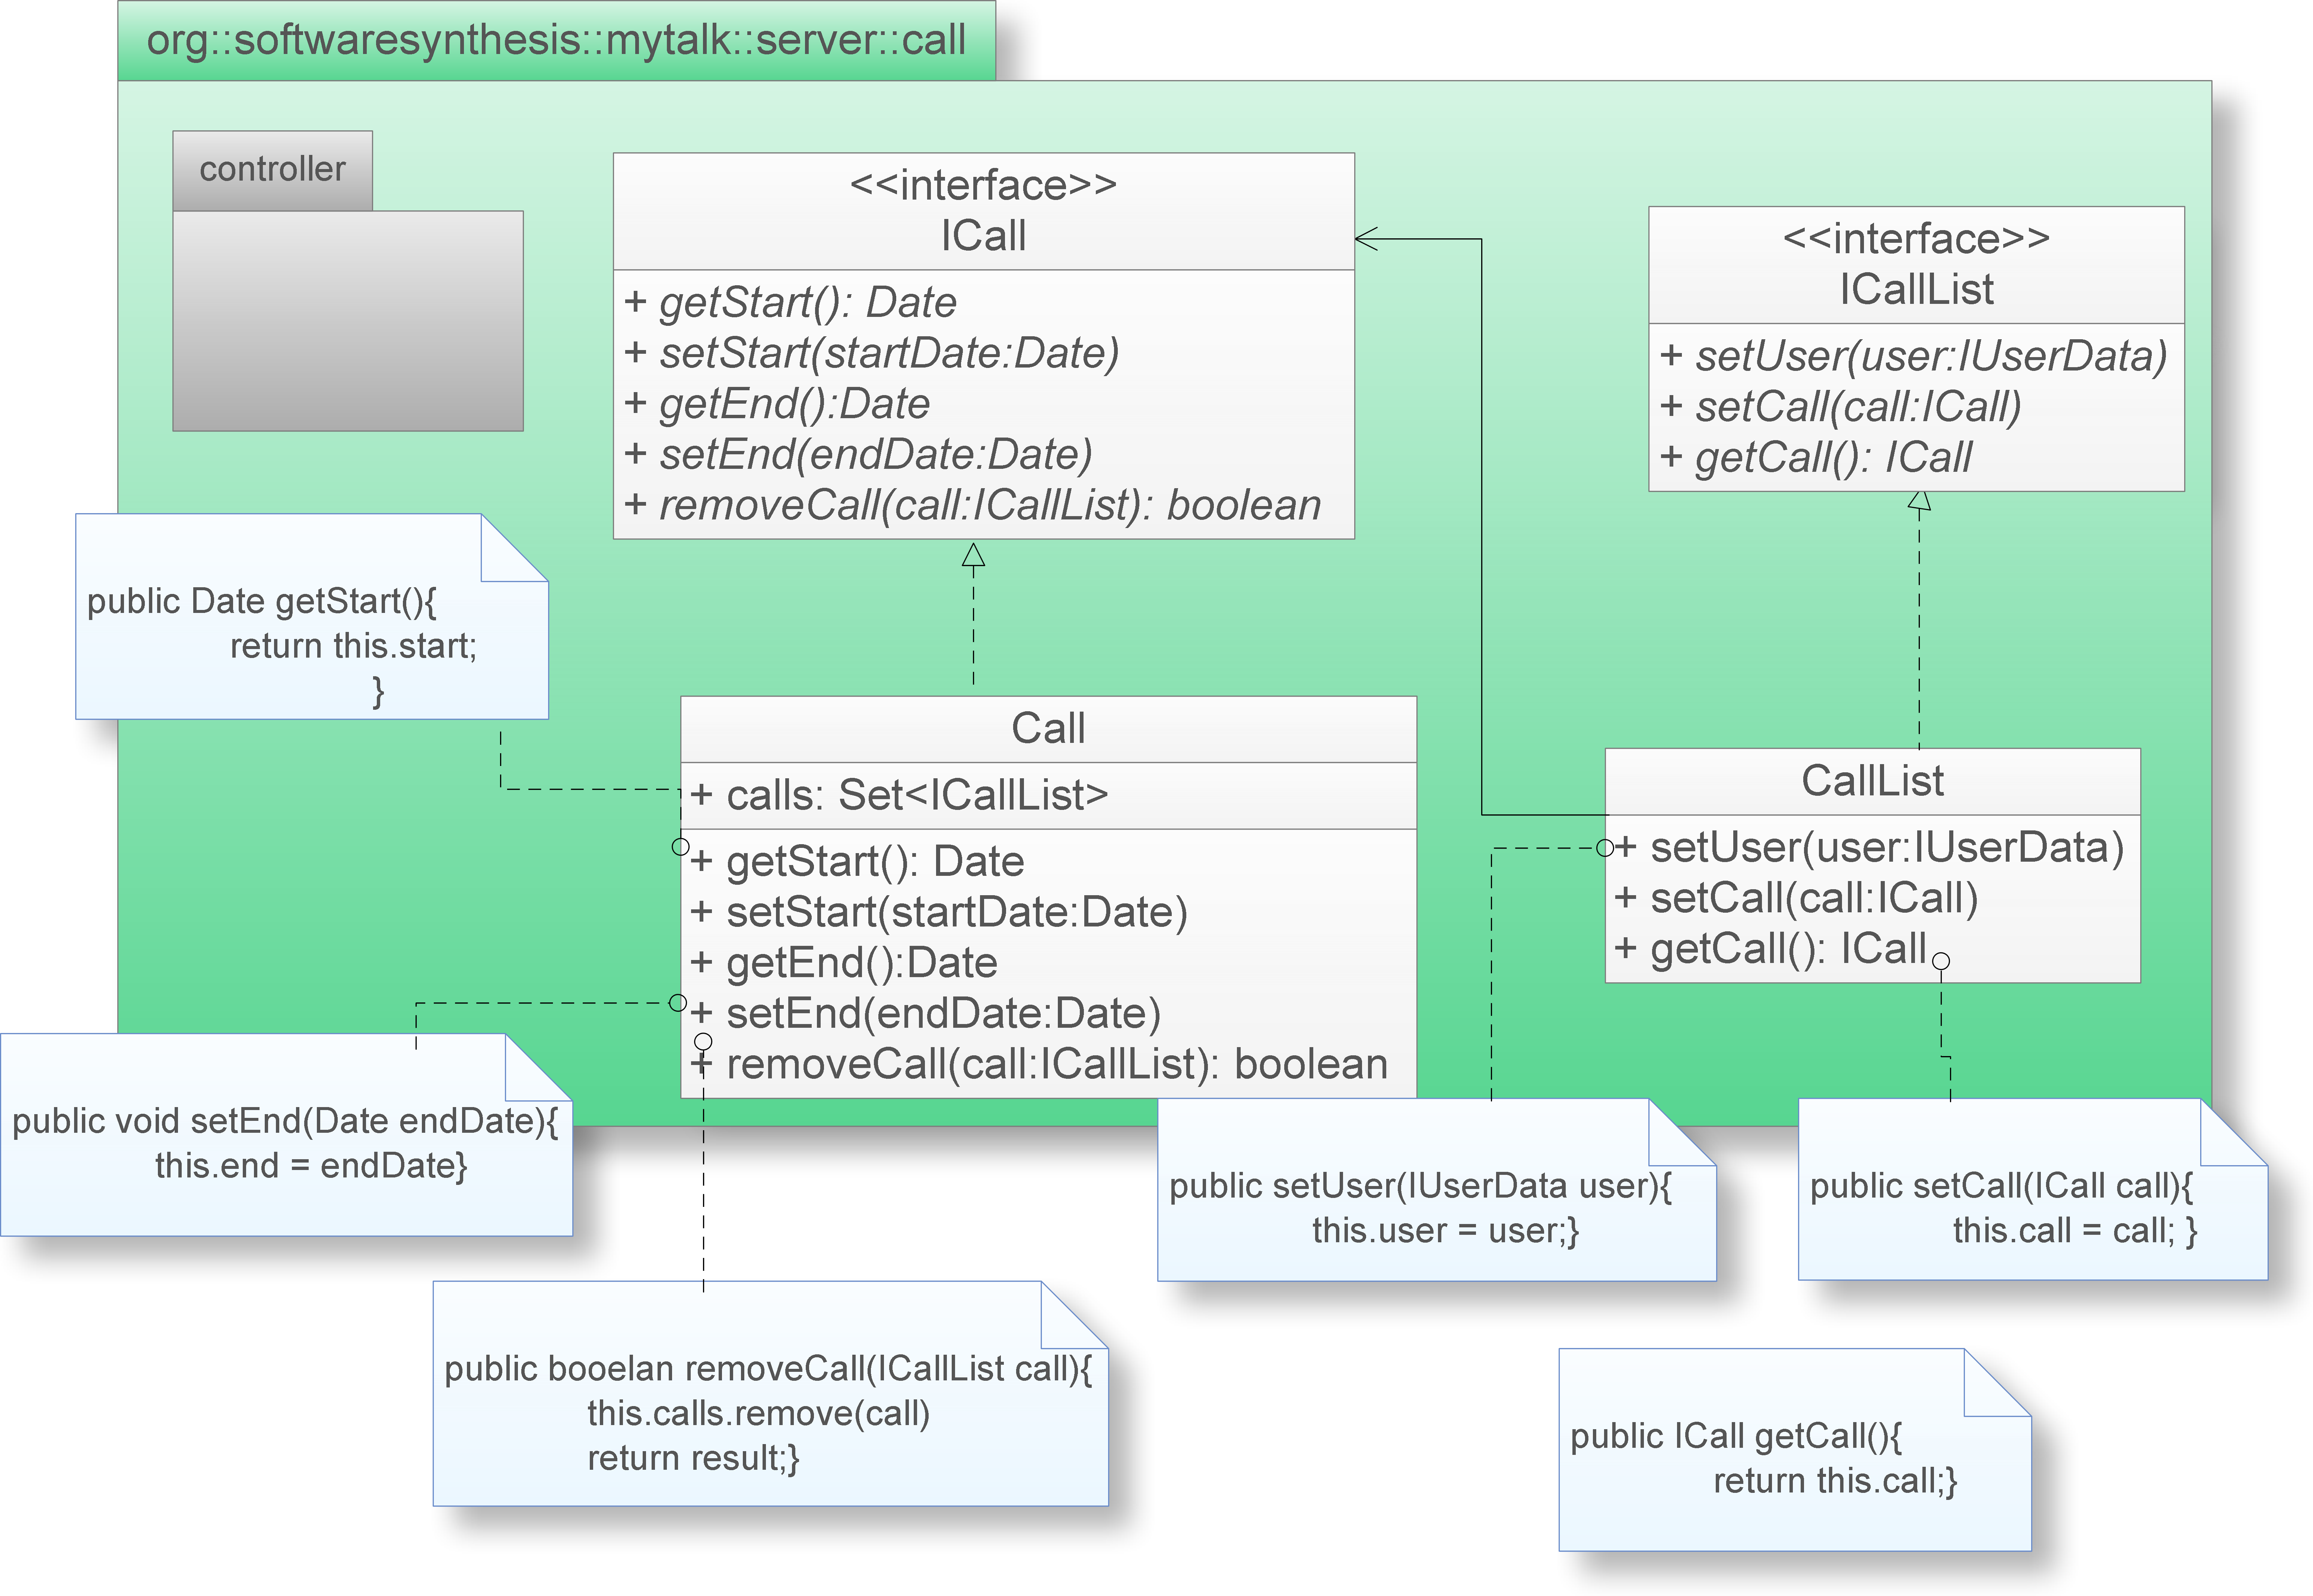
\includegraphics[width=\textwidth]{DDPCall}
%\caption{Diagramma package server.call}
%\end{figure}
%\end{center}

\classsection{PushInbound}

\subsubsection*{Funzione}
Classe per la definizione di un apposito canale di comunicazione client-server. La classe è un'estensione di \texttt{org.apache.catalina.websocket.MessageInbound}. Si osservi che l'associazione tra un istanza di \classname{PushInbound} e un utente del sistema è univoca: fintanto che connesso un utente ha un proprio \classname{PushInbound} presente sul server.

\subsubsection*{Relazioni d'uso}
\begin{itemize}
	\item \texttt{java.io.IOException}: Eccezione che può sollevare il metodo \method{OnTextMessage()}.
	\item \texttt{java.nio.CharBuffer}: tipologia di \textit{buffer} usata per memorizzare il messaggio ricevuto come parametro d'ingresso.
	\item \texttt{java.util.Iterator}: usata per scorrere il contenuto dell'insieme di \classname{AddressBookEntry}
	\item \texttt{java.util.Set}: struttura dati usata per memorizzare le \inglese{entry} (\classname{AddressBookEntry}) che costituiscono la rubrica dell'utente.
	\item \texttt{com.google.gson.*}: converte i dati interni in una stringa formato JSON.
	
	\item \classname{abook.AddressBookEntry}: usata per definire la rubrica dell'utente, richiamata dal metodo \method{onTextMessage} nel momento in cui si presenta la necessità di aggiornare lo stato dell'utente e renderlo visibile ai suoi contatti.
	\item \classname{abook.IUserData}: usata per riferire un istanza della classe ad un particolare utente.
	\item \classname{dao.DataPersistanceManger}: usata per riferire un istanza della classe ad un particolare utente.

\end{itemize}

\subsubsection*{Classi estese ed interfacce implementate}
\begin{itemize}
	\item \texttt{org.apache.catalina.websocket.MessageInbound}: classe da estendere, aggiunge alla classe \classname{PushInbound} le funzionalità necessarie per renderla un ``canale di comunicazione'' utilizzabile dai client.
\end{itemize}

\subsubsection*{Attributi}
\begin{description}
  \item{\memberdata{-- id: Long}}\\
  Identificativo di tipo \textit{Long} del canale di comunicazione associato ad un client univoco.
  \item{\memberdata{-- state: State}}\\
  Attributo usato per memorizzare lo stato dell'utente ``proprietario'' del \classname{PushInbound}.
\end{description}

%TODO da rivedere.

\subsubsection*{Metodi}
\begin{description}

	\item{\method{+ setId(n: Long): void}}\\
	Metodo per impostare il valore contenuto nell'attributo \memberdata{id}.
	
	\item{\method{+ getId(): Long}}\\
	Metodo che ritorna il contenuto dell'attributo \memberdata{id}.
	
	\item{\method{+ onTextMessage(message: CharBuffer): void}}\\
	Metodo invocato al momento della ricezione di un messaggio da parte del client. Il metodo riceve in input un oggetto di tipo \texttt{CharBuffer} contenente il messaggio inviato dal client.
Inizialmente il metodo crea un istanza per ognuno dei seguenti oggetti:
	\begin{itemize}
		\item[•]\texttt{Gson}: tipo di JSON definito da \textit{Google};
		\item[•]\texttt{JsonParser}: \textit{parser} usato per scorrere il contenuto di una stringa JSON;
		\item[•]\texttt{JsonArray}: array popolato a partire dal \inglese{parsing} della stringa di messaggio data in input.
	\end{itemize}
	
	Prima di procedere si voglia considerare quanto segue: il metodo dopo aver ``segmentato'' il messaggio ricevuto in input, si occupa di esaminarne il contenuto che può essere di 5 tipologie, ciascuna identificata tramite un valore intero positivo da 1 a 5. Tale valore deve essere salvato nell'istanza di \texttt{JsonArray}
	Detto ciò, tornando a definire il flusso principale del metodo, si osservi che:

	\begin{itemize}
		\item[•]Se la richiesta inoltrata è del tipo 1: il metodo prende in lettura il messaggio e imposta il contenuto di \memberdata{id} con il valore letto mediante procedura di \inglese{parsing} analoga a quella definita al passo precedente. Per farlo utilizza il metodo \texttt{fromJson} richiamato dall'istanza \texttt{gsonObj} di tipo \texttt{Gson} creata al passo precedente. A tale metodo passa il contenuto dell'array e in particolare ciò che è salvato nella posizione 1 (utilizzo di metodo \texttt{get(int i)}).
		\item[•]Se la richiesta inoltrata è del tipo 2: il metodo procede con le istruzioni necessarie a scambiare i dati per la chiamata. Nello specifico viene salvato in un attributo di tipo \texttt{Long}, l'\texttt{id} del client che desidero chiamare, quindi ricerco l'oggetto \texttt{PushInbound} associato al client che desidero contattare, e gli inoltro il messaggio ricevuto come parametro d'ingresso.
		\item[•]Se la richiesta inoltrata è del tipo 3: il metodo comunica al client ``destinatario'' della chiamata, l'\texttt{id} del client chiamante. La procedura è analoga a quella identificata nel punto precedente, con la specifica che il messaggio inoltrato è l'identificativo del cliente che desidera avviare la chiamata.
		\item[•]Se la richiesta inoltrata è del tipo 4: il metodo si occupa dell'eliminazione della \underline{WebSocket}.
		\item[•]Se la richiesta inoltrata è del tipo 5: il metodo viene usato per modificare lo stato dell'utente, con il valore passato tramite messaggio. Dopo la ricezione del messaggio, il metodo cambia il valore del campo \texttt{state} con il valore ricevuto come parametro d'ingresso. Quindi procede ricavando la lista degli utenti nella rubrica dell'utente che ha cambiato stato e comunica loro che è avvenuto un cambiamento di stato.
	\end{itemize}
\end{description}

\clearpage

\section{Specifica sotto-architettura \texttt{clientpresenter}}\label{sec:clientpresenterarchitecture}

La sotto-architettura \texttt{clientpresenter}\footnote{%
  Considerazioni in tutto e per tutto analoghe si applicano anche alla sotto-architettura \texttt{clientview} descritta nella sezione \vref{sec:clientviewarchitecture} del presente documento.
}
richiede una trattazione speciale a causa del particolare dominio tecnologico coinvolto. Essa è infatti definita con il linguaggio JavaScript che pur essendo definito come linguaggio orientato agli oggetti non permette di definire classi ed è, inoltre, debolmente tipizzato.

Al fine di facilitare al programmatore la comprensione del progetto (pensando quindi alle varie entità come a classi) senza però confonderlo in fase di stesura del codice, si è stabilito di adoperare la seguente terminologia:

\begin{description}
	\item{\scshape\bfseries Attributi}: saranno definiti con una sintassi simile a quella già usata per la parte server, pertanto al nome dell'attributo sarà associato il tipo ``logico'' che idealmente rappresenta. Dal momento che in JavaScript non esiste il controllo dei tipi, si è stabilito di attenersi a una notazione simile a quella utilizzata per lo strumento di generazione automatica della documentazione JSDoc. In particolare i tipi legali consentiti sono:
	\begin{itemize}
	  \item \texttt{HTMLElement} che corrispondono a nodi DOM già esistenti nella pagina HTML che definisce l'interfaccia utente oppure modificati (a \textit{run-time}) sulla base di informazioni ottenute dal server e che saranno indicati come:
	  	\begin{verbatim}
				(+, -) attributo: HTMLElement
			\end{verbatim}
	
    \item \texttt{String} se l'attributo è destinato a contenere esclusivamente valori di tipo \textit{String} che sarà segnato nel documento come:
			
			\begin{verbatim}
				(+, -) attributo: String
			\end{verbatim}
			
			\item \texttt{Array}, se l'attributo è un \inglese{array}, che in JavaScript non chiede di essere definito per tipo di valori contenibili che nel presente documento sarà segnalato come:
			
			\begin{verbatim}
				(+, -) attributo: Array
			\end{verbatim}
			
			\item \texttt{Number}, che è da considerarsi come il supertipo di tutti i tipi numerici e che sarà menzionato nel presente documento come:
			\begin{verbatim}
			  (+, -) attributo: Number
			\end{verbatim}
			
			\item \texttt{Boolean}, che rappresenta un valore booleano e che sarà indicato nel presente documento come:
			\begin{verbatim}
			  (+, -) attributo: Boolean
			\end{verbatim}
			
			\item \texttt{Object}, che è da intendersi come un oggetto generico JavaScript, dotato una serie di proprietà per ciascuna delle quali è definito un valore e che sarà rappresentato come:
			\begin{verbatim}
			  (+, -) attributo: Object
			\end{verbatim}
	\end{itemize}
		
Per quanto riguarda l'accessibilità degli attributi, invece, saranno distinti i due casi di accessibilità pubblica e accessibilità privata, indicati nel presente documento con un formalismo analogo a quello utilizzato per la parte server.

Nell'attività di codifica, i programmatori dovranno attenersi alle seguenti pratiche:
\begin{itemize}
  \item gli attributi pubblici saranno assimilati a proprietà dell'oggetto creato tramite la funzione costruttore accessibili all'esterno, e dovranno pertanto essere specificati come:
  \begin{verbatim}
    this.attributo = new ClassName();
  \end{verbatim}
  
  \item gli attributi privati invece, dal momento che saranno visibili solo all'interno del costruttore e di tutte le funzioni annidate all'interno di esso -- vale a dire i metodi della classe -- dovranno essere dichiarati come variabili locali secondo la consueta sintassi JavaScript:
  \begin{verbatim}
    var attributo = new ClassName();
  \end{verbatim}
\end{itemize}
		
	\item{\scshape\bfseries Metodi}: la sintassi usata dal programmatore per definire un metodo in JavaScript dipende dalla natura pubblica o privata del metodo stesso, in particolare:
	\begin{itemize}
	
\item i metodi pubblici possono essere assimilati in tutto e per tutto a delle proprietà che l'oggetto espone verso l'esterno, pertanto dovranno essere specificati come:
\begin{verbatim}
  this.doSomething = function(arg0, arg1, ...) {
          ...corpo del metodo...
  }
\end{verbatim}

\item i metodi privati, invece, essendo utilizzabili solo all'interno di altri metodi della classe, possono essere definiti come funzioni annidate all'interno del costruttore della classe stessa, secondo la consueta sintassi
\begin{verbatim}
  function doSomething(arg0, arg1, ...) {
        ...corpo del metodo...
  }
\end{verbatim}

La sintassi utilizzata all'interno del presente documento, in ogni caso, rimane quella che è stata definita in precedenza e prevede i marcatori \verb|+| per i metodi pubblici e \verb|-| per i metodi privati.

Per quanto concerne il tipo di ritorno, nel caso in cui non fosse previsto alcun valore da restituire, esso sarà indicato nel presente documento con la parola chiave \texttt{void}, analogamente a come sono stati trattati i metodi nella sotto-architettura \texttt{server}.

Qualora, infine, il metodo dovesse sollevare eccezioni mediante il costrutto JavaScript
\begin{verbatim}
  throw "error";
\end{verbatim}
nel presente documento sarà utilizzato il tipo generico \exception{Exception} specificando di volta in volta il messaggio di diagnostica contenuto nell'eccezione.

	\end{itemize}
\end{description}

\subsection{Package \texttt{org.softwaresynthesis.mytalk.clientpresenter.guicontrol}}\label{sec:guicontrol}

\begin{center}
\begin{figure}[H]
  \includegraphics[width=\textwidth]{DDPGuiControl}
\caption{Diagramma package clientpresenter.guicontrol}
\end{figure}
\end{center}

\classsection{AccountSettingsPresenter}
\subsubsection*{Funzione}
\inglese{Presenter} incaricato di gestire il pannello delle impostazioni e dei dati personali dell'utente visualizzando i dati inseriti in fase di registrazione e permettendo di modificarli in un secondo momento.

\subsubsection*{Relazioni d'uso}
\begin{itemize}
  \item \texttt{clientview.AccountSettingsView}: vista controllata da questo \inglese{presenter}.
\end{itemize}

\subsubsection*{Classi estese ed interfacce implementate}
Nessuna relazione evidenziata.

\subsubsection*{Attributi}
\begin{description}
\item{\memberdata{-- thisPanel: HTMLElement}}\\
Attributo che rappresenta un riferimento all'elemento HTML, da intendersi come nodo DOM, che rappresenta la radice del pannello associato a questo \inglese{presenter} ed è costituito da un \verb'<div>' avente come identificativo la stringa \verb'AccountSettingsPanel'.
\end{description}

\subsubsection*{Metodi}
\begin{description}

\item{\method{+ onShowAccountSettingPanel(): void}}\\
Questo gestore di eventi viene attivato al verificarsi dell'evento \verb'showAccountSettingPanel' e determina il caricamento del \inglese{template} che corrisponde al pannello delle impostazioni utente, demandando in un secondo momento alla vista il compito di inizializzare il comportamento del pannello mediante il metodo \method{display()} che essa mette a disposizione.

\item{\method{+ sendUserData(data: Object): Boolean}}\\
Il metodo ha il compito di gestire la modifica dell'utente ai propri dati verificando innanzitutto se essi hanno subito qualche variazione rispetto a quanto noto in precedenza, mediante una chiamata al metodo \method{hasSomethingChanged}. In caso affermativo, dovrà essere inviata una richiesta all'indirizzo del \inglese{front controller} per trasferire la modifica sui dati salvati sul database del server.

A tale scopo dovrà essere creata una nuova istanza di \verb'XMLHttpRequest' per effettuare una richiesta AJAX sincrona, con particolare attenzione a utilizzare un'istanza di \inglese{form data} dal momento che dovranno essere spediti anche dati di natura non testuale, con una sintassi del tipo:
\begin{verbatim}
  var form = new FormData();
  formData.append("operation", "accountSettings");
        ...altri valori da inviare...
  var request = new XMLHttpRequest();
  request.open("POST", controllerURL, false);
  request.send(form);
\end{verbatim}

Da ultimo, il metodo dovrà restituire il valore ottenuto deserializzando il testo della risposta ottenuta dal server, che è \verb'true' se l'operazione è andata a buon fine e \verb'false' altrimenti.

\item{\method{-- hasSomethingChanged(data: Object): Boolean}}\\
L'oggetto passato come parametro in ingresso a questo metodo è costituito dalle proprietà \verb'name', \verb'surname' e \verb'picturePath' che rappresentano gli unici dati utente che sono suscettibili di possibili modifiche. Il metodo dovrà restituire \verb'true' se almeno una di queste proprietà ha un valore diverso rispetto alle informazioni che sono memorizzate nel client  e \verb'false' altrimenti.

\end{description}


\classsection{AddressBookPresenter}

\subsubsection*{Funzione}
\inglese{Presenter} incaricato di gestire il pannello della rubrica che controlla i \inglese{widget} grafici relativi alla vista e ha la responsabilità di aggiornarla sulla base dei dati ricevuti dal server.

\subsubsection*{Relazioni d'uso}
\begin{itemize}
  \item \texttt{clientview.AddressBookView}: vista controllata da questo \inglese{presenter}.
\end{itemize}

\subsubsection*{Classi estese ed interfacce implementate}
Nessuna relazione evidenziata.

\subsubsection*{Attributi}
\begin{description}
  
   \item{\memberdata{-- contacts: Object}}\\
  Attributo che rappresenta la lista degli utenti presenti nella rubrica. Tale attributo è rappresentato da un array associativo indicizzato in base all'identificativo di ciascun contatto i cui valori sono oggetti che rappresentano contatti, e ha una rappresentazione in formato JSON del tipo:
  \begin{verbatim}
  {
  	"id0": {
  	        "id": "id0",
  	        "name": "Mario",
  	        "surname": "Rossi",
            "email": "indirizzo1@dominio.it",
            "picturePath": "img/contactImg/Default.png",
            "state": "available",
            "blocked": false
  	       },
  	"id1": {
  	        "id": "id1",
  	        "name": "Giuseppe",
  	        "surname": "Verdi",
            "email": "indirizzo2@dominio.it",
            "picturePath": "img/contactImg/Default.png",
            "state": "offline",
            "blocked": false
  	       }
  }
  \end{verbatim}
  
   \item{\memberdata{-- groups: Object}}\\
  Attributo che definisce la lista dei gruppi presenti nella rubrica dell'utente che ha effettuato l'autenticazione.
  
  Tale attributo è rappresentato da un array associativo indicizzato in base all'identificativo di ciascun gruppo, di cui sono elencati il nome e i contatti in forma di array enumerativo, secondo un formato JSON del tipo:
  \begin{verbatim}
  {
  	"id0": {
  	        "id": "id0",
  	        "name": "addrBookEntry",
  	        "contacts": [0, 1, 2, 3]
  	       },
  	"id1": {
  	        "id": "id1",
  	        "name": "someName",
  	        "contacts": [1, 2]
  	       }
  }
  \end{verbatim}
  
   \item{\memberdata{-- thisPanel: HTMLElement}}\\
  Riferimento all'elemento, da intendersi come nodo DOM, che rappresenta il pannello controllato da questo \inglese{presenter} che nello specifico è rappresentato da un \verb'<div>' con l'identificativo \verb'AddressBookPanel'.
  
\end{description}

\subsubsection*{Metodi}
\begin{description}

\item{\method{+ applyFilterByGroup(idGroup: Number): Object}}\\
Il metodo ha il compito di restituire al chiamante un array associativo di contatti, indicizzato in base all'identificativo univoco degli stessi, aventi la proprietà di essere tutti e soli contatti che appartengono al gruppo avente come identificativo il valore intero passato come parametro.

Tale insieme di contatti può essere ottenuto iterando sugli identificativi contenuti nella proprietà \verb'contacts' del gruppo e inserendo in un array associativo l'elemento \memberdata{contacts}\verb'[i]' in corrispondenza della chiave \verb'i'.

\item{\method{+ applyFilterByString(param: String): Object}}\\
Questo metodo ha il compito di restituire sotto forma di array associativo indicizzato per l'identificativo di ciascun contatto l'insieme dei contatti tali che soddisfano un determinato criterio di ricerca testuale passato come parametro.

A tale scopo dovranno quindi essere creati un array inizialmente vuoto e una nuova espressione regolare corrispondente al parametro di ricerca con l'istruzione
\begin{verbatim}
  var pattern = new RegExp(param);
\end{verbatim}

In seguito, dovrà essere eseguito un ciclo su tutti i contatti contenuti nell'attributo \memberdata{contacts} aggiungendo all'array iniziale qualsiasi contatto le cui proprietà \verb'name', o \verb'surname' oppure \verb'email' soddisfi il test con l'espressione regolare.

Infine, dal momento che soddisfa i requisiti richiesti dal chiamante, l'array così popolato dovrà essere restituito al chiamante.

\item{\method{+ getContact(idContact: Number): Object}}\\
Il metodo dovrà restituire il contatto della rubrica che ha come valore identificativo l'intero passato come parametro. Tale risultato può essere ottenuto accedendo all'oggetto corrispondente nell'array associativo \memberdata{contacts} dal momento che gli identificativi sono le chiavi su cui è indicizzato.

\item{\method{+ getContacts(): Object}}\\
Fornisce al chiamante l'insieme dei contatti che sono presenti nella rubrica dell'utente restituendo un riferimento all'oggetto memorizzato nella variabile di istanza \memberdata{contacts}.

\item{\method{+ getGroups(): Object}}\\
Fornisce al chiamante l'insieme dei gruppi che sono presenti nella rubrica dell'utente restituendo un riferimento all'oggetto memorizzato nella variabile di istanza \memberdata{groups}.

\item{\method{+ getGroupsWhereContactsIs(contact:Object): Object}}\\
Tale metodo dovrà restituire un array associativo con la stessa struttura interna del campo dati \memberdata{groups} contenente l'insieme di tutti i gruppi cui appartiene il contatto passato come parametro.

All'interno del corpo del metodo dovrà pertanto essere definito un nuovo array associativo, quindi dovrà essere realizzato un ciclo su tutti i gruppi della rubrica e, all'interno di ciascun gruppo, dovrà essere scorsa la proprietà \verb'contacts' per determinare se fra gli identificativi ivi contenuti si trova l'id del contatto da cercare.

In tal caso il gruppo dovrà essere aggiunto all'array definito nel metodo che, al termine del ciclo principale, conterrà tutti e soli i gruppi desiderati e potrà essere restituito al chiamante.

\item{\method{+ onAddContactToAddressBook(contact: Object): Boolean}}\\
Questo gestore di eventi ha il compito di verificare se nella rubrica dell'utente esiste già il contatto ricevuto come parametro in ingresso con un'invocazione del metodo privato \method{contactAlreadyPresent}. 

In caso negativo, il metodo dovrà procedere inviando una richiesta AJAX sincrona al server per provocare l'aggiunta del contatto alla rubrica dell'utente creando una nuova istanza di \verb'XMLHttpRequest' con la \inglese{query string}
\begin{verbatim}
    "operation=addContact&contactId=" + contact.id
\end{verbatim}

Poiché il server ritorna la stringa \verb'"true"' se l'operazione va a buon fine, è sufficiente che il metodo restituisca \texttt{true} se il risultato di \verb'JSON.parse(request.responseText)' è valutato positivamente e \verb'false' in caso contrario. Inoltre, nel caso in cui il contatto sia stato aggiunto con successo, dovrà essere richiamato il metodo \method{setup()} del \inglese{presenter}.

In caso di terminazione con errore della procedura nel server oppure nell'eventualità in cui il contatto che si richiede di aggiungere alla rubrica sia già presente, il metodo dovrà sollevare due \exception{Exception} contenenti, rispettivamente, il messaggio ``Errore nel server'' e ``Contatto già presente in rubrica''.

\item{\method{+ onAddContactToGroup(contact: Object, group: Object): Boolean}}\\
Questo gestore di eventi ha il compito di verificare che il contatto passato come primo parametro non sia già presente nel gruppo passato come secondo parametro tramite il metodo privato \method{contactExistInGroup} e, in caso negativo, inviare una richiesta AJAX sincrona al server per provocare l'aggiunta del contatto all'interno del gruppo della rubrica, creando una nuova istanza di \verb'XMLHttpRequest' con la \inglese{query string}
\begin{verbatim}
"operation=addInGroup&contactId=" + contact.id + "&groupId=" + group.id
\end{verbatim}

Poiché il server ritorna la stringa \verb'"true"' se l'operazione va a buon fine, è sufficiente che il metodo restituisca \verb'true' se il risultato di \verb'JSON.parse(request.responseText)' è valutato positivamente e \verb'false' in caso contrario. Inoltre, nel caso in cui il contatto sia stato aggiunto con successo al gruppo, dovrà essere richiamato il metodo \method{setup()} fornito dal \inglese{presenter} stesso.

In caso di errore oppure nell'eventualità in cui il contatto che si richiede di aggiungere alla rubrica sia già presente, il metodo dovrà sollevare due \exception{Exception} contenenti, rispettivamente, il messaggio ``Errore nel server'' e ``Contatto già presente nel gruppo''.

\item{\method{+ onBlockContact(contact: Object): Boolean}}\\
Questo gestore di eventi ha il compito di verificare se il contatto passato come parametro non è presente in rubrica oppure se è già bloccato (verificando la proprietà \verb'contact.blocked') e, in caso negativo, inviare una richiesta AJAX sincrona al server per provocare il blocco del contatto. A tal fine dovrà essere predisposta una nuova istanza di \verb'XMLHttpRequest' da inviare all'indirizzo del \inglese{front controller} con la \inglese{query string}
\begin{verbatim}
    "operation=blockContact&contactId=" + contact.id
\end{verbatim}

Poiché il server ritorna la stringa \verb'"true"' se l'operazione va a buon fine, è sufficiente che il metodo restituisca \verb'true' se il risultato di \verb'JSON.parse(request.responseText)' è valutato positivamente e \verb'false' in caso contrario. Inoltre, nel caso in cui il contatto sia stato bloccato, dovrà essere richiamato il metodo \method{setup()} del \inglese{presenter}.

In caso di errore da parte del server, o di richiesta di bloccare un contatto inesistente, oppure nell'eventualità in cui il contatto di cui si richiede il blocco sia già bloccato, il metodo dovrà sollevare tre \exception{Exception} contenenti, rispettivamente, il messaggio ``Errore nel server'', ``Contatto non presente in rubrica'' e ``Contatto già bloccato''.

\item{\method{+ onChangeAddressBooksContactState(contact: Object, state: String): void}}\\
Questo gestore di eventi è richiamato nel momento in cui si riceve una notifica di cambiamento di stato relativa a un contatto. Il metodo dovrà innanzitutto controllare che il contatto passato come primo parametro sia presente nella rubrica, quindi aggiornare la proprietà \verb'state' di quest'ultimo in maniera corrispondente.

In seguito sarà responsabilità del \inglese{presenter} aggiornare la vista in modo che lo stato visualizzato nell'interfaccia utente corrisponda a quello reale, mediante una chiamata al metodo \method{setState} reso disponibile dalla vista.

\item{\method{+ onCreateGroup(name: String): Boolean}}\\
Questo gestore di eventi ha il compito di verificare se nella rubrica dell'utente esiste già un gruppo con nome uguale a quello passato come parametro iterando sui valori contenuti nell'array associativo \memberdata{groups} e confrontando la loro proprietà \verb'name' con il valore del parametro.

In caso negativo, dovrà provvedere all'invio di una richiesta AJAX sincrona al server per provocare l'aggiunga del nuovo gruppo, creando a tale scopo una nuova istanza di \verb'XMLHttpRequest' con la seguente \inglese{query string}
\begin{verbatim}
    "operation=addGroup&groupName=" + group.name
\end{verbatim}

Poiché il server ritorna la stringa \verb'"true"' se l'operazione va a buon fine, è sufficiente che il metodo restituisca \verb'true' se il risultato di \verb'JSON.parse(request.responseText)' è valutato positivamente e \verb'false' in caso contrario. Inoltre, nel caso in cui il gruppo sia stato effettivamente creato, dovrà essere richiamato il metodo \method{setup()} del \inglese{presenter}.

In caso di errore nel server oppure nell'eventualità in cui il gruppo che si richiede di creare esista già, il metodo dovrà sollevare due \exception{Exception} contenenti, rispettivamente, il messaggio ``Errore nel server'' e ``Gruppo già presente''.

\item{\method{+ onDeleteGroup(group: Object): Boolean}}\\
Questo gestore di eventi avrà il compito di verificare che il gruppo passato come parametro esista realmente nella rubrica dell'utente iterando sulle chiavi dell'array associativo \memberdata{groups} confrontandole con la proprietà \verb'id' del gruppo passato come parametro.

In caso affermativo, e solo in tale caso, il metodo dovrà inviare una richiesta AJAX sincrona al server per provocarne la cancellazione creando a tale fine una nuova istanza di \verb'XMLHttpRequest' con la seguente \inglese{query string}
\begin{verbatim}
    "operation=deleteGroup&groupId=" + group.id
\end{verbatim}

Poiché il server ritorna la stringa \verb'"true"' se l'operazione va a buon fine, è sufficiente che il metodo restituisca \verb'true' se il risultato di \verb'JSON.parse(request.responseText)' è valutato positivamente e \texttt{false} in caso contrario. Inoltre, nel caso in cui il gruppo sia stato effettivamente rimosso, dovrà essere richiamato il metodo \method{setup()} del \inglese{presenter}.

In caso di errore nel server oppure nell'eventualità in cui il gruppo che si richiede di eliminare non esista, il metodo dovrà sollevare due \exception{Exception} contenenti, rispettivamente, il messaggio ``Errore nel server'' e ``Impossibile eliminare gruppo inesistente''.

\item{\method{+ onRemoveAddressBookPanel(): void}}\\
Questo gestore di eventi ha il compito di provocare la distruzione del pannello per la visualizzazione della rubrica dell'utente, richiamando il metodo \method{destroy()} messo a disposizione dalla vista corrispondente.

\item{\method{+ onRemoveContactFromAddressBook(contact: Object): Boolean}}\\
Questo gestore di eventi ha il compito verificare che il contatto passato come parametro sia effettivamente presente nella rubrica dell'utente mediante un'invocazione del metodo \method{contactAlreadyPresent} e, solo in caso affermativo, di inviare una richiesta AJAX sincrona al server per provocare la rimozione del contatto dalla rubrica. A tal fine dovrà essere predisposta una nuova istanza di \verb'XMLHttpRequest' con la \inglese{query string}
\begin{verbatim}
  "operation=deleteContact&contactId=" + contact.id
\end{verbatim}

Poiché il server ritorna la stringa \verb'"true"' se l'operazione va a buon fine, è sufficiente che il metodo restituisca \verb'true' se il risultato di \verb'JSON.parse(request.responseText)' è valutato positivamente e \texttt{false} in caso contrario. Inoltre, nel caso in cui il contatto sia stato effettivamente rimosso dalla rubrica, dovrà essere richiamato il \method{setup()} del \inglese{presenter}.

In caso di errore nel server oppure nell'eventualità in cui il contatto che si richiede di rimuovere dalla rubrica non è già presente, il metodo dovrà sollevare due \exception{Exception} contenenti, rispettivamente, il messaggio ``Errore nel server'' e ``Impossibile eliminare contatto non presente in rubrica''.

\item{\method{+ onRemoveContactFromGroup(contact: Object, group: Object): Boolean}}\\
Questo gestore di eventi avrà il compito innanzitutto di verificare che il contatto passato come primo parametro sia effettivamente presente nel gruppo passato come secondo parametro, mediante una chiamata al metodo privato \method{contactExistInGroup}.

Esclusivamente in caso affermativo, dovrà essere inviata una richiesta AJAX sincrona all'indirizzo del server per provocare l'effettiva rimozione del contatto, creando una nuova istanza di \verb'XMLHttpRequest' con la seguente \inglese{query string}
\begin{verbatim}
"operation=deleteContact&contactId=" + contact.id + "&groupId=" + group.id
\end{verbatim}

Dato che il server ritorna la stringa \verb'"true"' se l'operazione va a buon fine, è sufficiente che il metodo restituisca \verb'true' se il risultato di \verb'JSON.parse(request.responseText)' è valutato positivamente e \verb'false' in caso contrario. Inoltre, nel caso in cui il contatto sia stato rimosso con successo dal gruppo, dovrà essere richiamato il metodo \method{setup()}.

In caso di errore nel server oppure nell'eventualità in cui il contatto che si richiede di rimuovere dal gruppo non vi appartenga, il metodo dovrà sollevare due \exception{Exception} contenenti, rispettivamente, il messaggio ``Errore nel server'' e ``Impossibile eliminare contatto non presente nel gruppo''.

\item{\method{+ onShowAddressBookPanel(): void}}\\
Questo gestore di evento ha il compito di provocare la visualizzazione dei \inglese{widget} grafici che costituiscono il pannello della rubrica, determinando il caricamento del \inglese{template} corrispondente e demandando in un secondo momento alla vista il compito di inizializzarsi.

\item{\method{+ onUnlockContact(contact: Object): Boolean}}\\
Questo gestore di eventi dovrà innanzitutto verificare che il contatto passato come parametro sia effettivamente presente nella rubrica (mediante il metodo \method{contactAlreadyPresent}) e che non sia già stato in precedenza sbloccato controllando la proprietà \verb'blocked' del contatto.

In caso affermativo, e solo allora, il metodo avrà il compito di inviare una richiesta AJAX sincrona al server per rimuovere il blocco dal contatto passato come parametro, creando una nuova istanza di \verb'XMLHttpRequest' con la \inglese{query string}
\begin{verbatim}
    "operation=unblockContact&contactId=" + contact.id
\end{verbatim}

Poiché il server ritorna la stringa \verb'"true"' se l'operazione va a buon fine, è sufficiente che il metodo restituisca \verb'true' se il risultato di \verb'JSON.parse(request.responseText)' è valutato positivamente e \verb'false' in caso contrario. Inoltre, nel caso in cui il contatto sia stato effettivamente sbloccato, dovrà essere richiamato il metodo \method{setup()} del \inglese{presenter}.

In caso di errore, o di richiesta di sbloccare un contatto non presente in rubrica oppure nell'eventualità in cui il contatto di cui si richiede lo sblocco è già stato sbloccato, il metodo dovrà sollevare tre \exception{Exception} contenenti, rispettivamente, il messaggio ``Errore nel server'', ``Contatto non presente in rubrica'' e ``Contatto già sbloccato''.

\item{\method{+ setup(): void}}\\
Il metodo ha il compito di scaricare dal server i dati necessari al funzionamento del \inglese{presenter} e in secondo momento passare alla vista le informazioni necessarie per popolare il pannello nel formato di cui quest'ultima necessita.

Dovrà essere pertanto richiamato il metodo privato \method{getAddressBookData()}, per poi richiamare le due operazioni \method{initializeContactList()} e \method{initializeGroupSelect()} messe a disposizione della vista. Per ogni contatto presente in rubrica dovrà quindi essere chiamato il metodo \method{addListItem} e per ogni gruppo dovrà essere richiamato il metodo \method{addOptionToSelect}, entrambi messi a disposizione dalla vista.

\item{\method{-- contactAlreadyPresent(contact): Boolean}}
Il metodo dovrà restituire \verb'true' se il contatto passato come parametro appartiene alla rubrica dell'utente e \verb'false' altrimenti. Tale controllo dovrà essere effettuato con un ciclo sui valori contenuti nell'array \memberdata{contacts} e confrontando le proprietà \verb'id' dei contatti.

\item{\method{-- contactExistInGroup(contact: Object, group: Object): Boolean}}\\
Restituisce il valore \verb'true' se il contatto passato come primo parametro in ingresso appartiene al gruppo passato come secondo parametro, \verb'false' altrimenti.

Il metodo dovrà pertanto ciclare fra tutti gli identificativi presenti nella proprietà \verb'contacts' del gruppo e, nel momento in cui dovesse trovare un valore uguale a \verb'contact.id' restituire \verb'true', mentre restituire \verb'false' nel caso in cui il ciclo termini per esaurimento degli elementi contenuti in \verb'group.contacts'.

\item{\method{-- getAddressBookData(): void}}\\
Tale metodo ha il compito di recuperare l'insieme dei contatti e dei gruppi presenti nella rubrica dell'utente per inizializzare in maniera corretta i campi dati \memberdata{contacts} e \memberdata{groups} rispettivamente.
  
  A tal fine dovranno essere inviate due richieste AJAX sincrone all'indirizzo del \inglese{front controller} presente sul server creando due opportune nuove istanze di \verb'XMLHttpRequest' che dovranno contenere nella \inglese{query string} il parametro \verb'operation' uguale, rispettivamente, a \verb'getContacts' e \verb'getGroups'.

\end{description}


\classsection{CallHistoryPresenter}

\subsubsection*{Funzione}
\inglese{Presenter} incaricato alla visualizzazione e alla gestione dello storico chiamate dell'utente.

\subsubsection*{Relazioni d'uso}
\begin{itemize}
  \item \texttt{clientview.CallHistoryView}: vista controllata da questo \inglese{presenter}.
\end{itemize}

\subsubsection*{Classi estese ed interfacce implementate}
Nessuna relazione evidenziata.

\subsubsection*{Attributi}
\begin{description}
  \item{\memberdata{-- calls: Array}}\\
  Array enumerativo che conterrà tutte le chiamate effettuate dall'utente recuperate dal server la cui struttura è rappresentata in formato JSON dalla seguente stringa
  \begin{verbatim}
  [
    {
      "id" : 0
      "email" : "indirizzo1@dominio.it",
      "start": "Wed May 22 12:42:42 CEST 2013",
      "caller": true
    },
    {
      "id" : 1,
      "email" : "indirizzo2@dominio.it",
      "start": "Thu May 23 21:42:42 CEST 2013",
      "caller": true
    }
  ]
  \end{verbatim}
  
  
  \item{\memberdata{-- thisPanel: HTMLElement}}\\
  Elemento HTML, da intendersi come nodo DOM, che rappresenta la vista controllata da questo \inglese{presenter} e che corrisponde a un elemento \verb'<div>' avente come nome identificativo la stringa \verb'CallHistroryPanel'.
\end{description}

\subsubsection*{Metodi}
\begin{description}

  \item{\method{+ displayList(): void}}\\
  Metodo che ha il compito di popolare la lista delle chiamate in cui è coinvolto un determinato utente. Il metodo ha il compito di procurarsi la lista delle chiamate attraverso il server al fine di inizializzare il campo dati privato \verb'calls'.
  
  Quindi, per ognuna delle chiamate che sono state scaricate, ha il compito di aggiornare la vista corrispondente provocando la visualizzazione dei dati della chiamata mediante il metodo \verb'addListItem' messo a disposizione da quest'ultima.
  
  \item{\method{+ onShowCallHistoryPanel(): void}}\\
  Questo gestore di eventi ha il compito di provocare la visualizzazione del pannello contenente lo storico delle chiamate demandando alla vista il compito di costruirsi e caricare il relativo \inglese{template}.
  
    \item{\method{-- getCalls(): Array}}\\
  Metodo che ha il compito di recuperare tutta la lista delle chiamate effettuate e tracciate nel server, inviando una richiesta AJAX sincrona al \inglese{front controller} che nell'intestazione contiene il parametro \verb'operation' impostato a \verb'getCalls'.
  
  In particolare, il metodo ha il compito di creare una nuova istanza di \verb'XMLHttpRequest' con la \inglese{query string} specificata in precedenza e di inviarla al server quindi ritornare il testo della risposta ottenuta dopo averlo deserializzato e costruito l'array di chiamate corrispondente.

\end{description}


\classsection{CommunicationPresenter}
\subsubsection*{Funzione}
Questo \inglese{presenter} ha il compito di gestire tutte le comunicazioni che possono avvenire tra persone, quindi sia di natura testuale che di tipo audio oppure audio/video.

\subsubsection*{Relazioni d'uso}
\begin{itemize}
  \item \texttt{clientview.CommunicationView}: vista controllata da questo \inglese{presenter};
  \item \texttt{clientpresenter.kernelCommunicationCenter}: per gestire le chiamate in ingresso/uscita.
\end{itemize}

\subsubsection*{Classi estese ed interfacce implementate}
Nessuna relazione evidenziata.

\subsubsection*{Attributi}
\begin{description}

  \item{\memberdata{-- audio: Object}}\\
  Mappa associativa di oggetti creati con una chiamata al costruttore \verb'new Audio(fileName)' le cui chiavi corrispondono alle stringhe \verb'"income"' e \verb'"outcome"' cui sono associati i suoni per il segnale di chiamata in arrivo e di chiamata in uscita rispettivamente.
  
  \item{\memberdata{-- intervalRing: Object}}\\
  Intervallo impostato inizialmente a \verb'null' nel costruttore e in seguito inizializzato di volta in volta dal gestore di evento \method{onStartRinging} che permette di controllare (e di arrestare) la riproduzione del segnale di chiamata.
  
\item{\memberdata{-- thisPanel: HTMLElement}}\\
Riferimento all'elemento HTML, da intendersi come nodo DOM, che corrisponde alla radice del pannello per la visualizzazione delle comunicazioni ed è costituito, ai fini pratici, da un elemento \verb'<div>' avente l'identificativo \verb'CommunicationPanel'.

\end{description}

\subsubsection*{Metodi}
\begin{description}

  \item{\method{+ getMyVideo(): HTMLElement}}\\
  Il metodo dovrà restituire un riferimento l'elemento DOM con l'identificativo ad\verb'myVideo' presente nel pannello delle comunicazioni.

  \item{\method{+ getOtherVideo(): HTMLElement}}\\
  Il metodo dovrà restituire un riferimento l'elemento DOM con l'identificativo ad\verb'otherVideo' presente nel pannello delle comunicazioni.
  
  \item{\method{+ onAppendMessageToChat(user: Object, message: String, amISender: Boolean)}}\\
  Questo gestore di eventi ha il compito di aggiungere il messaggio di testo passato come secondo parametro all'elemento che rappresenta la chat testuale aperta con l'utente passato come primo parametro, in maniera corretta rispetto al fatto che l'utente del client sia o meno il mittente del messaggio. A tale fine dovrà essere richiamato il metodo \method{appendToChat} messo a disposizione dalla vista associata a questo \inglese{presenter}.
  
  %FIXME questo sicuramente non sarà corretto! Controllare per favore!
  \item{\method{+ onCall(user: Object, onlyAudio: Boolean): void}}\\
  Questo gestore di eventi viene richiamato al verificarsi di un evento con stringa identificativa \verb'call' che segnala l'avvio di una comunicazione audio (secondo parametro a \verb'true') o audio/video (secondo parametro a \verb'false') con l'utente passato come primo parametro.
  Al verificarsi di un simile evento, il \inglese{presenter} dovrà contattare l'istanza presente di \classname{CommunicationCenter} e invocare il metodo \method{call} di quest'ultimo con il primo parametro a \verb'true' e inoltrando i valori di \verb'contact' e \verb'onlyAudio' come secondo e terzo parametro.
  
  \item{\method{+ onChatStarted(user: Object): void}}\\
  Questo gestore di eventi viene richiamato quando si avvia una comunicazione testuale con il contatto passato come parametro. A tal fine dovrà essere invocato il metodo \method{addChat} messo a disposizione dalla vista associata a questo \inglese{presenter}.
  
  \item{\method{+ onShowCommunicationPanel(): void}}\\
  Questo gestore di eventi avrà il compito di provocare la visualizzazione del pannello per la gestione delle comunicazioni, provocando il caricamento del \inglese{template} corrispondente, la sua aggiunta nel punto corretto dell'albero DOM e demandando in un secondo momento alla vista il compito dell'inizializzazione dei \inglese{widget} grafici che lo costituiscono.
  
  \item{\method{+ onStartRinging(evt: String): void}}\\
  Questo gestore di eventi ha il compito di avviare il trillo che segnala una chiamata in arrivo (se il parametro è uguale a \verb'"income"') oppure il segnale di attesa di risposta (se il parametro è uguale a \verb'"outcome"').
  
  A tal fine dovrà essere utilizzata la funzione di libreria \verb'setInterval', salvando il risultato dell'invocazione della funzione nel campo dati \memberdata{intervalRing}. Il secondo parametro da passare alla funzione sarà l'intervallo di \inglese{timeout} pari a 1000 (per determinare la riproduzione ciclica del suono ogni secondo), mentre la funzione anonima passata come primo parametro dovrà invocare il metodo \verb'play()' sull'elemento \verb'Audio' corrispondente, in base al valore del parametro \verb'evt' ricevuto dal metodo.
  
  \item{\method{+ onStopRinging(): void}}\\
  Questo gestore di eventi dovrà determinare l'interruzione della riproduzione del suono che segnala una chiamata in uscita oppure in entrata. A tal fine dovrà essere utilizzata la funzione di libreria \verb'clearInterval' passando come parametro l'attributo \memberdata{intervalRing}, quindi impostare quest'ultimo al valore \verb'null'.

\end{description}


\classsection{ContactPresenter}

\subsubsection*{Funzione}
\inglese{Presenter} incaricato di gestire il pannello per la visualizzazione di un contatto, sia esso della rubrica che un generico utente del sistema non presente in rubrica.

\subsubsection*{Relazioni d'uso}
\begin{itemize}
  \item \texttt{clientview.ContactView}: vista controllata da questo \inglese{presenter}.
\end{itemize}

\subsubsection*{Classi estese ed interfacce implementate}
Nessuna relazione evidenziata.

\subsubsection*{Attributi}
\begin{description}

  \item{\memberdata{-- thisPanel: HTMLElement}}\\
  Riferimento all'elemento HTML, da intendersi come nodo DOM, che rappresenta la radice del pannello per la visualizzazione di un contatto. Quest'ultimo è costituito concretamente da un elemento \verb'<div>' con l'identificativo \verb'ContactPanel'.
  
\end{description}

\subsubsection*{Metodi}
\begin{description}

  \item{\method{+ onRemoveContactPanel(): void}}\\
  Questo gestore di eventi dovrà eseguire le operazioni che dovranno essere richiamate quando il pannello per la visualizzazione dei dati di un contatto viene rimosso e, in particolare, dovrà impostare a \verb'null' il valore del campo dati \memberdata{currentContact}.
  
  \item{\method{+ onShowContactPanel(contact: Object): void}}\\
  Questo gestore di eventi ha il compito di provocare la visualizzazione del pannello del profilo del contatto passato come parametro, caricando il \inglese{template} HTML presente sul server, inizializzando il valore dell'attributo \memberdata{currentContact} e demandando in un secondo momento alla vista il compito di inizializzarsi tramite il metodo \method{display}.
  
\end{description}


\classsection{GroupPresenter}

\subsubsection*{Funzione}
\inglese{Presenter} incaricato di gestire il pannello per la visualizzazione e l'amministrazione dei gruppi presenti nella rubrica.

\subsubsection*{Relazioni d'uso}
\begin{itemize}
  \item \texttt{clientview.GroupView}: vista controllata da questo \inglese{presenter}.
\end{itemize}

\subsubsection*{Classi estese ed interfacce implementate}
Nessuna relazione evidenziata.

\subsubsection*{Attributi}
\begin{description}

  \item{\memberdata{-- contacts: Object}}\\
  Array associativo in cui sono memorizzati i contatti della rubrica, indicizzato in base al numero identificativo di ciascun contatto.
  
  \item{\memberdata{-- groups: Object}}\\
  Array associativo in cui sono memorizzati i gruppi presenti nella rubrica, indicizzato in base al numero identificativo di ciascun gruppo.
  
  \item{\memberdata{-- thisPanel: Object}}\\
  Riferimento all'elemento HTML, da intendersi come nodo DOM, che rappresenta il pannello controllato dal \inglese{presenter} ed è costituito da un \verb'<div>' con l'identificativo \verb'GroupPanel'.
  
\end{description}

\subsubsection*{Metodi}
\begin{description}

  \item{\method{+ displayList(): void}}\\
  Metodo che visualizza all'interno del pannello la lista dei gruppi presenti in rubrica. A tale scopo è necessario innanzitutto inizializzare i campi dati \memberdata{contacts} e \memberdata{groups}, quindi è possibile popolare la vista mediante una chiamata al metodo \method{addListItem} messo a disposizione dalla vista per ognuno dei gruppi che sono stati precedentemente recuperati.
  
  \item{\method{+ onShowGroupPanel(): void}}\\
  Questo gestore di eventi è associato all'evento con l'identificativo \verb'showGroupPanel' e determina la visualizzazione del pannello per l'amministrazione dei gruppi della rubrica caricando il relativo \inglese{template} e demandando in un secondo momento alla vista il compito di inizializzare le proprie componenti grafiche.
  
  \item{\method{+ selectCandidates(group: Object): Object}}\\
  Il metodo ha il compito di estrarre dall'insieme di tutti i contatti memorizzati nella rubrica quelli che non appartengono al gruppo passato come parametro e che, pertanto, sono dei candidati per l'aggiunta allo stesso.
  
  L'algoritmo mediante il quale dovrà essere raggiunto questo scopo consiste nell'effettuare una copia \textit{profonda} dell'array associativo dei contatti presenti in rubrica, che costituirà l'insieme dei candidati da restituire al chiamante.
  
  In seguito, si dovrà scorrere la proprietà \verb'contacts' del gruppo (che è un array enumerativo dei numeri identificativi dei contatti che vi appartengono) e rimuovere gli oggetti corrispondenti dall'array dei candidati con l'istruzione \verb'delete'.
  
  Al termine del \inglese{loop}, l'array associativo così ottenuto conterrà solo i contatti che non appartengono al gruppo come richiesto e potrà quindi essere restituito al chiamante.

\end{description}


\classsection{LoginPresenter}

\subsubsection*{Funzione}
\inglese{Presenter} incaricato di gestire il pannello di \textit{login}, ha il compito di recuperare i dati inseriti dall'utente (\textit{username} e \textit{password}) dall'interfaccia grafica, controllare se assumono dei valori legali e in seguito passarli al server per eseguire l'autenticazione.

Il \inglese{presenter} si occupa inoltre di gestire il caso in cui l'autenticazione non può essere portata a termine per errori nei dati di input e fornisce infine le funzionalità per il recupero della \textit{password}.

\subsubsection*{Relazioni d'uso}
\begin{itemize}
  \item \texttt{clientview.LoginView}: vista controllata da questo \inglese{presenter}.
\end{itemize}

\subsubsection*{Classi estese ed interfacce implementate}
Nessuna relazione evidenziata.

\subsubsection*{Attributi}
\begin{description}

\item{\memberdata{-- thisPanel: HTMLElement}}\\
Attributo che definisce il contenuto del nodo DOM inerente alla schermata di \inglese{login}, nello specifico tale nodo corrisponde ad un \verb+<div>+ il cui valore identificativo è uguale a \texttt{LoginPanel}.

\end{description}

\subsubsection*{Metodi}
\begin{description}

\item{\method{+ getUsername(): String}}\\
Metodo che ha il compito di recuperare tramite l'interfaccia della vista il nome utente inserito dall'utente, quindi effettuare un controllo preliminare per assicurare che il valore rientri all'interno del dominio dei valori legali.

Il controllo dovrà essere effettuato mediante un'opportuna espressione regolare del tipo:
\begin{verbatim}
  ^[A-Z0-9._%+-]+@[A-Z0-9.-]+\.[A-Z]{2,4}$
\end{verbatim}
e, nel caso in cui il valore non corrispondesse, il metodo dovrà sollevare una \exception{Exception} contenente il testo ``indirizzo email non valido''. Dal momento che il metodo restituisce una stringa, in caso di valore accettabile quest'ultimo dovrà essere restituito al chiamante.

\item{\method{+ getPassword(): String}}\\
Metodo che ha il compito di recuperare tramite l'interfaccia della vista la \textit{password} inserita dall'utente. Prima di restituire il valore ottenuto al chiamante, il metodo ha il compito di verificare che il valore sia valido e che, in particolare, non sia \verb+undefined+ oppure uguale alla stringa vuota. In simili circostanze, il metodo solleva una \exception{Exception} contenente esattamente il testo ``password non specificata''.

\item{\method{+ getSecretQuestion(username: String): String}}\\
Il metodo a il compito di richiedere al server tramite una chiamata AJAX sincrona la domanda segreta associata all'utente che ha come nome identificativo la stringa passata come parametro, e restituirla al chiamante.

Al suo interno dovrà essere creata pertanto una nuova istanza di \verb+XMLHttpRequest+ destinata all'indirizzo del \inglese{front controller} presente sul server, e dovrà essere inviata  passando al metodo \verb+send+ la stringa:
\begin{verbatim}
  "operation=question&username=" + encodeURIComponent(username)
\end{verbatim}

Dal momento che il testo della risposta ricevuta dal server contiene la domanda segreta, sarà infine sufficiente restituire il valore ottenuto con \verb+request.responseText+.

\item{\method{+ login(data: Object): String}}\\
Il metodo prende come parametro un oggetto dotato delle due proprietà \verb+usename+ e \verb+password+ sulla base delle quali avrà il compito di costruire la \inglese{query string} da inviare al server per la verifica delle credenziali.

Il metodo dovrà pertanto costruire una \verb+XMLHttpRequest+ da inviare all'indirizzo del \inglese{front controller} presente sul server con la stringa
\begin{verbatim}
    operation=login&username=" + encodeURIComponent(data.username) +
                  "&password=" + encodeURIComponent(data.password)
\end{verbatim}
quindi invocare il già visto metodo \verb+testCredentials+ con il testo della risposta. Il valore da restituire al chiamante è proprio la stringa di \inglese{query} che è stata trasmessa al server.

\item{\method{+ onLogin(user: Object): void}}\\
Questo gestore di evento incapsula il comportamento del \inglese{presenter} nel momento in cui è sollevato un evento avente come identificativo la stringa \verb'login'.

Il metodo ha il compito di memorizzare all'interno del client i dati di autenticazione (in particolare, il valore numerico ID necessario all'identificazione del client da parte del server e degli altri client), avviare la connessione al server e provocare la visualizzazione della \inglese{home screen} dell'applicativo.

\item{\method{+ onRemoveLoginPanel() : void}}\\
Questo gestore di evento ha il compito di provocare la distruzione del pannello di autenticazione, richiamando il metodo \method{destroy()} della vista corrispondente.

\item{\method{+ onShowLoginPanel(): void}}\\
Questo gestore di evento ha il compito di provocare la visualizzazione del pannello di login. Questo dovrà essere ottenuto sollevando un nuovo evento tramite il quale tutti i pannelli presenti sono rimossi (\verb'removeAllPanel') quindi demandando alla vita il compito di costruirsi e caricare il relativo \inglese{template}.

\item{\method{-- hasAnsweredCorrectly(username: String, answer: String): void}}\\
Il metodo ha il compito di inviare la risposta ottenuta tramite l'interfaccia grafica al server per verificare se corrisponde al valore memorizzato nel database del sistema in fase di registrazione iniziale. In particolare, il metodo ha il compito di inviare una richiesta AJAX sincrona all'indirizzo del \inglese{front controller} la cui intestazione è la stringa
\begin{verbatim}
  "operation=answer&username=" + username + "&answer=" + answer
\end{verbatim}

Una volta ricevuta la risposta, poiché questa già corrisponde alla stringa \verb+true+ o \verb+false+ che rappresentano le costanti booleane in formato JSON, sarà sufficiente restituirne la valutazione ottenuta con la consueta funzione \verb+parse+.

\item{\method{-- testCredentials(data: String): void}}\\
Il metodo prende come parametro una stringa JSON ricevuta dal server che, in caso di dati di autenticazione andata a buon fine, corrisponde a una forma serializzata dell'oggetto che rappresenta l'utente autenticato ed è invece uguale alla stringa \verb+null+ in caso contrario.

Il metodo ha il compito di deserializzare i dati dell'utente tramite la funzione di libreria \verb+JSON.parse(data)+ e, nel caso in cui questa sia valutata positivamente -- vale a dire non è né \verb+null+ né \verb+undefined+ -- sollevare un evento avente come nome la stringa \verb'login' e come proprietà \verb+user+ un riferimento al nuovo utente creato.

In caso di autenticazione non andata a buon fine, invece, dovrà essere aggiornata in modo opportuno la vista per segnalare la condizione di errore.

\end{description}


\classsection{MainPresenter}

\subsubsection*{Funzione}
\inglese{Presenter} incaricato di gestire il pannello principale, ossia quello che occupa la regione centrale.

\subsubsection*{Relazioni d'uso}
\begin{itemize}
  \item \texttt{clientview.MainView}: vista controllata da questo \inglese{presenter}.
\end{itemize}

\subsubsection*{Classi estese ed interfacce implementate}
Nessuna relazione evidenziata.

\subsubsection*{Attributi}
\begin{description}
\item{\memberdata{-- thisPanel: HTMLElement}}\\
  Riferimento all'elemento controllato dal \inglese{presenter} vale a dire un \verb'<div>' avente come identificativo la stringa \verb'MainPanel'.
\end{description}

\subsubsection*{Metodi}
\begin{description}

  \item{\method{+ onRemoveMainPanel(): void}}\\
  Questo gestore di eventi è richiamato nel momento in cui è sollevato un evento con nome identificativo \texttt{removeMainPanel} e ha il compito di richiamare il metodo \method{destroy()} della vista corrispondente.
  
  \item{\method{+ onShowGeneralPanel(panel: String): void}}\\
  Gestore di eventi che ha il compito di aggiornare la vista associata a questo \inglese{presenter} tramite il metodo \method{displayChildPanel} per la visualizzazione di un generico contenuto HTML (ricevuto come parametro) all'interno del pannello principale.
  
  \item{\method{+ onShowMainPanel(): void}}\\
  Questo gestore di eventi è richiamato nel momento in cui è sollevato un evento avente come nome identificativo la stringa \texttt{showMainPanel} e ha il compito di provocare il caricamento del \inglese{template} del pannello e, in seguito, di demandare al metodo \method{display()} della vista la sua inizializzazione.

\end{description}


\classsection{MessagePresenter}

\subsubsection*{Funzione}
\inglese{Presenter} incaricato di gestire i messaggi in segreteria che permette di scaricarli dal server, eliminarli e impostarne lo stato.

\begin{itemize}
  \item \texttt{clientview.MessageView}: vista controllata da questo \inglese{presenter}.
\end{itemize}

\subsubsection*{Classi estese ed interfacce implementate}
Nessuna relazione evidenziata.

\subsubsection*{Attributi}
\begin{description}
 \item{\memberdata{-- messages: Array}}\\
 Array destinato a contenere la lista dei messaggi della segreteria il cui destinatario è l'utente del client.

 \item{\memberdata{-- thisPanel: HTMLElement}}\\
  Riferimento all'elemento HTML, da intendersi come nodo DOM, che rappresenta il pannello della segreteria ed è concretamente un \verb'<div>' con identificativo uguale a \verb'MessagePanel'.
\end{description}

\subsubsection*{Metodi}
\begin{description}

  \item{\method{+ deleteMessage(message: Object) Boolean}}\\
  Elimina un messaggio dalla segreteria inviando all'indirizzo del \inglese{front controller} del server una richiesta AJAX sincrona tramite un'istanza di \verb'XMLHttpRequest' che contiene la \inglese{query string}
  \begin{verbatim}
    "operation=deleteMessage&idMessage=" + message.id
  \end{verbatim}
  
  Poiché il server restituisce le stringhe \verb'"true"' o \verb'"false"' che corrispondono alla rappresentazione in formato JSON delle omonime costanti letterali del linguaggio, sarà sufficiente che il metodo restituisca il risultato dell'espressione \verb'JSON.parse(request.responseText)'. In caso di errore, inoltre, dovrà comparire un messaggio d'errore indicante il motivo.
  
    \item{\method{+ displayList(): void}}\\
  Tale metodo ha il compito di popolare la vista con i messaggi della segreteria telefonica provvedendo in primo luogo a scaricarli dal server mediante il metodo \method{getMessages()} al fine di inizializzare l'attributo \memberdata{messages}, quindi aggiornare la vista in maniera corrispondente invocando per ognuno dei messaggi scaricati in precedenza il metodo \method{addListItem} messo a disposizione dalla vista.
  
    \item{\method{+ onShowMessagePanel(): void}}\\
  Questo gestore di eventi viene attivato al verificarsi dell'evento \verb'showMessagePanel' e determina il caricamento del \inglese{template} che corrisponde al pannello della segreteria telefonica, demandando in un secondo momento alla vista il compito di inizializzare il comportamento del pannello chiamando il metodo \method{display()} messo a disposizione dalla vista.
  
    \item{\method{+ setStatus(message: Object, valueToSet: Boolean): Boolean}}\\
  Imposta lo stato di un messaggio come ``nuovo'' oppure ``già letto'' a seconda del parametro ricevuto in input. Tale metodo ha il duplice compito di modificare lo stato del messaggio ricevuto come parametro in base al valore di \verb'valueToSet' e quindi inviare una richiesta AJAX sincrona al server che contiene la \inglese{query string}
  \begin{verbatim}
    "operation=updateMessage&idMessage=" + message.id +
               "&read=" + valueToSet
  \end{verbatim}
  
  Poiché il server restituisce le stringhe \verb'"true"' o \verb'"false"' che corrispondono alla rappresentazione in formato JSON delle omonime costanti letterali del linguaggio, sarà sufficiente che il metodo restituisca il risultato dell'espressione \verb'JSON.parse(request.responseText)'.
  
    \item{\method{-- getMessages(): Array}}\\
  Ottiene i messaggi di segreteria salvati nel server creando una nuova \verb'XMLHttpRequest' da inviare all'indirizzo del \inglese{front controller} del server per realizzare una richiesta AJAX sincrona nella cui \inglese{query string} dovrà obbligatoriamente essere presente il parametro \verb'operation', con una sintassi del tipo:
  \begin{verbatim}
    request.send("operation=getMessages");
  \end{verbatim}
  
  Dal momento che il server risponde con la versione serializzata in JSON della lista di messaggi desiderata, il metodo dovrà limitarsi a restituire il risultato dell'invocazione di \verb'JSON.parse(request.responseText)'.
  
\end{description}


\classsection{PresenterMediator}

\subsubsection*{Funzione}
L'unica istanza di tale classe presente nel client ha il compito di coordinare la collaborazione, potenzialmente complessa, fra tutti i \inglese{presenter} che gestiscono l'interfaccia grafica permettendo lo scambio di informazioni fra gli stessi ed evitando che ognuno di essi debba riferire direttamente gli altri.

\subsubsection*{Relazioni d'uso}
L'istanza di questa classe si trova ad utilizzare, per coordinare la loro interazione, un riferimento a tutti e dodici i\inglese{presenter} che sono stati definiti, vale a dire:
\begin{itemize}
  \item \texttt{clientpresenter.guicontrol.AccountSettingsPresenter};
  \item \texttt{clientpresenter.guicontrol.AddressBookPresenter};
  \item \texttt{clientpresenter.guicontrol.CallHistoryPresenter};
  \item \texttt{clientpresenter.guicontrol.CommunicationPresenter};
  \item \texttt{clientpresenter.guicontrol.ContactPresenter};
  \item \texttt{clientpresenter.guicontrol.GroupPresenter};
  \item \texttt{clientpresenter.guicontrol.LoginPresenter};
  \item \texttt{clientpresenter.guicontrol.MainPresenter};
  \item \texttt{clientpresenter.guicontrol.MessagePresenter};
  \item \texttt{clientpresenter.guicontrol.RegisterPresenter};
  \item \texttt{clientpresenter.guicontrol.SearchResultPresenter};
  \item \texttt{clientpresenter.guicontrol.ToolsPresenter}.
\end{itemize}

\subsubsection*{Classi estese ed interfacce implementate}
Nessuna relazione evidenziata.

\subsubsection*{Attributi}
\begin{description}

  \item{\memberdata{-- views}}\\
  Mappa associativa i cui chiavi e le cui valori sono rappresentati da tipi \verb'String', che permette di associare gli identificativi delle viste ai relativi \inglese{template} HTML che devono essere caricati mediante il metodo \method{getView}.
  
  Essendo il contenuto di questo oggetto interamente determinato in maniera statica, è possibile fornirne una rappresentazione in formato JSON che corrisponde a:
  \begin{verbatim}
  {
      "accountSettings" : "AccountSettingsView.html",
      "addressBook" : "AddressBookView.html",
      "callHistory" : "CallHistoryView.html",
      "contact" : "ContactView.html",
      "communication" : "CommunicationView.html",
      "group" : "GroupView.html",
      "login" : "LoginView.html",
      "main" : "MainView.html",
      "message" : "MessageView.html",
      "phoneCallsRegistry" : "PhoneCallsRegistryView.html",
      "register" : "RegisterView.html",
      "searchResult" : "SearchResultView.html",
      "tools" : "ToolsView.html"
  }
  \end{verbatim}
  
  \item{\memberdata{-- presenters}}\\
  Array associativo che contiene i riferimenti a tutti i \inglese{presenter} di primo livello come valori, utilizzando il medesimo insieme di chiavi descritto in dettaglio per l'attributo \memberdata{views}.
  
  Alla chiave \verb'login' dovrà pertanto corrispondere una nuova istanza di \classname{LoginPresenter} inizializzata all'interno del costruttore della classe \classname{PresenterMediator} con l'istruzione
\begin{verbatim}
  new LoginPresenter();
\end{verbatim}
e così via per ciascuno dei cinque presenter di primo livello, vale a dire:
\begin{itemize}
  \item[--] \classname{LoginPresenter};
  \item[--] \classname{RegisterPresenter};
  \item[--] \classname{MainPresenter};
  \item[--] \classname{AddressBookPresenter};
  \item[--] \classname{ToolsPresenter};
\end{itemize}
in modo che in seguito sia possibile ottenere un'istanza del \inglese{presenter} semplicemente utilizzando la notazione \verb'presenters["login"]', \verb'presenters["addressBook"]' e così via.
  
  \item{\memberdata{-- secondaryPresenters}}\\
Tale campo dati ha il compito di memorizzare in un array associativo i riferimenti ai sette \inglese{presenter} di secondo livello, indicizzati secondo le stesse stringhe che sono state utilizzate per le viste all'interno del campo dai \memberdata{views}.

L'inizializzazione di questo campo dati dovrà avvenire all'interno del metodo costruttore di \classname{PresenterMediator} in maniera del tutto analoga a quanto descritto per la variabile di istanza \memberdata{presenters} e dovrà riguardare, in particolare:
\begin{itemize}
  \item[--] \classname{AccountSettingsPresenter}; 
  \item[--] \classname{CallHistoryPresenter}; 
  \item[--] \classname{CommunicationPresenter}; 
  \item[--] \classname{ContactPresenter};
  \item[--] \classname{GroupPresenter};
  \item[--] \classname{MessagePresenter};
  \item[--] \classname{SearchResultPresenter}.
\end{itemize}

Anche in questo caso, all'interno dei metodi della classe sarà possibile riferire i vari \inglese{presenter} utilizzando una notazione del tipo \verb'secondarypresenters["contact"]' oppure \verb'secondarypresenters["communication"]'.
  
\end{description}

\subsubsection*{Metodi}

\begin{description}

\item{\method{+ contactAlreadyPresent(contact: Object): Boolean}}\\
Tale metodo dovrà restituire \verb'true' se il contatto passato come parametro appartiene già alla rubrica dell'utente e \verb'false' altrimenti. Il valore desiderato può essere ottenuto mediante una semplice invocazione del metodo omonimo messo a disposizione da \classname{AddressBookPresenter}.

\item{\method{+ createNameLabel(contact: Object): String}}\\
Il metodo ha il compito di restituire la rappresentazione in formato stringa del nome del contatto passato come parametro, da utilizzarsi ogni volta che un contatto dovrà essere visualizzato nell'interfaccia grafica (ad esempio nella rubrica, fra i risultati di una ricerca, come mittente di un messaggio in segreteria oppure contatto coinvolto in una chiamata nello storico).

La rappresentazione testuale di un contatto deve contenere almeno una voce tra i valori di \verb'contact.name' e \verb'contact.surname', se almeno uno dei due è specificato oppure, se non sono disponibili i dati anagrafici del contatto da visualizzare, l'indirizzo email di quest'ultimo.

\item{\method{+ getAddressBookContacts(): Object}}\\
Tale metodo ha il compito di restituire tutti i contatti presenti nella rubrica dell'utente rappresentati come un array associativo con una struttura analoga a quella della variabile privata \memberdata{contacts} contenuta in \classname{AddressBookPresenter}. Un simile oggetto può essere ottenuto mediante il metodo pubblico \method{getContacts()} fornito da \classname{AddressBookPresenter}.

\item{\method{+ getAddressBookGroups(): Object}}\\
Tale metodo ha il compito di restituire l'insieme dei gruppi presenti nella rubrica dell'utente rappresentati come un array associativo con una struttura analoga a quella della variabile privata \memberdata{groups} contenuta in \classname{AddressBookPresenter}. Un simile oggetto può essere ottenuto mediante un'invocazione del metodo pubblico \method{getGroups()} messo a disposizione da \classname{AddressBookPresenter}.

\item{\method{+ getContactById(idContact: Number): Object}}\\
Il metodo dovrà restituire il contatto della rubrica che è caratterizzato dal numero intero identificativo passato come parametro. A tal fine è possibile invocare il metodo \method{getContact} che è reso disponibile da \classname{AddressBookPresenter}.

\item{\method{+ getGroupsWhereContactIs(contact: Object): Object}}\\
Tale metodo avrà il compito di restituire l'insieme di tutti e soli i gruppi della rubrica dell'utente tali che il contatto passato come parametro vi appartiene, in formato di mappa associativa dalla struttura analoga a quella del campo dati \memberdata{groups} di \classname{AddressBookPresenter}. Un oggetto di questo tipo può essere ottenuto mediante l'invocazione del metodo omonimo messo a disposizione dal \inglese{presenter} per la gestione del pannello della rubrica.

\item{\method{+ getMyVideo(): HTMLElement}}\\
Questo metodo dovrà restituire un riferimento all'elemento \verb'<video>' che nel pannello della comunicazione corrisponde alla visualizzazione del flusso multimediale proveniente dal client dell'utente finale dell'applicativo. Un simile riferimento può essere ottenuto mediante l'invocazione del metodo pubblico omonimo messo a disposizione dal \classname{CommunicationPresenter}.

\item{\method{+ getOtherVideo(): HTMLElement}}\\
Questo metodo dovrà restituire un riferimento all'elemento \verb'<video>' che nel pannello della comunicazione corrisponde alla visualizzazione del flusso multimediale proveniente dal client dell'utente remoto con cui si è instaurata una comunicazione. Un simile riferimento può essere ottenuto mediante l'invocazione del metodo pubblico omonimo messo a disposizione dal \classname{CommunicationPresenter}.

\item{\method{+ getView(key: String): void}}\\
Questo metodo ha il compito di ottenere dal server un frammento XHTML che rappresenta la porzione di codice corrispondente al pannello della vista, che in seguito dovrà essere gestita in una fase preliminare dal metodo \method{onLoadedView} di questa stessa classe, e in una fase successiva dagli \method{initialize} delle viste di primo livello e dai \method{display()} delle viste di secondo livello.

Al fine di scaricare dal server il \inglese{template} del pannello, questo metodo dovrà inviare una nuova richiesta AJAX sincrona all'indirizzo del server tramite un'opportuna istanza di \verb'XMLHttpRequest', richiedendo tramite il metodo HTTP GET la risorsa il cui URI relativo è dato dalla concatenazione della stringa \verb'"clientview/"' con il valore presente nell'attributo \memberdata{views} in corrispondenza dell'indice dato dal parametro \verb'key' del metodo stesso.

Dopo aver inviato la richiesta mediante il metodo di libreria \verb'send()', dovrà essere invocato il metodo di utilità (privato) \verb'onLoadedView' di questo stesso presenter, passando come primo parametro la chiave identificativa del \inglese{presenter} detinatario (\texttt{key}) e come secondo parametro il testo scaricato dal server (cioè la proprietà \texttt{response}) della richiesta.

\item{\method{+ onRemoveAllPanel(): void}}\\
Questo gestore di eventi dovrà determinare la scomparsa dall'interfaccia grafica di tutte le viste di primo livello visualizzate. A tale scopo dovranno essere quindi sollevati i cinque eventi corrispondenti (su cui le viste sono in ascolto), vale a dire \verb'removeLoginPanel', \verb'removeRegistrationPanel', \verb'removeAddressBookPanel', \verb'removeToolsPanel' e, da ultimo, \verb'removeMainPanel'.

\item{\method{+ onShowUIPanels(): void}}\\
Questo gestore di eventi avrà il compito di far visualizzare l'interfaccia grafica principale a seguito di un'autenticazione avvenuta con successo. A tale fine dovrà essere sollevato innanzitutto un evento con stringa identificativa uguale a \verb'removeAllPanels', quindi dovranno essere sollevati in sequenza i tre eventi \verb'showAddressBookPanel', \verb'showMainPanel' e \verb'showToolsPanel' che avviano i relativi \inglese{presenter} e fanno visualizzare i pannelli.

\item{\method{-- onLoadedView(presenter: String, view: String): void}}\\
Questo metodo privato ha il compito di gestire il caricamento di una delle viste che compongono l'interfaccia grafica. Il suo comportamento dovrà pertanto differenziarsi a seconda del fatto che si tratti di una vista di primo o di secondo livello o non appartenga a nessuno dei due casi, in base al valore del primo parametro che identifica il \inglese{presenter} destinatario.

Nel caso di una vista di primo livello, dovrà essere richiamato il metodo \method{initialize} messo a disposizione dalla vista stessa, passando la stringa HTML ricevuta come secondo parametro per la visualizzazione e l'inizializzazione della vista.

Nel caso invece di una vista di secondo livello, sarà responsabilità del metodo far visualizzare la vista nel pannello centrale tramite il metodo \method{displayChildPanel} della \classname{MainView}, demandando poi alla specifica vista l'inizializzazione delle componenti tramite il metodo \method{display} corrispondente.

Infine, se il primo parametro non corrisponde ad alcuno dei \inglese{presenter} di primo o di secondo livello, allora dovrà essere visualizzato un pannello temporaneo il cui contenuto HTML interno corrisponde a quanto ricevuto come secondo parametro dal metodo.

A tale scopo dovrà pertanto essere creato un \verb'<div>' con l'identificativo \verb'overlayPopUp' che dovrà essere aggiunto come primo figlio dell'elemento \verb'<body>' e un secondo \verb'<div>' con identificativo \verb'popUp' che dovrà essere aggiunto immediatamente dopo l'\inglese{overlay} dopo aver assegnato il valore del parametro \verb'view' al contenuto HTML interno di quest'ultimo. Tutti gli altri eventuali figli del \verb'<body>' dovranno essere posizionati in successivamente nell'albero DOM con un'istruzione del tipo \verb'body.insertBefore(overlay, bodyFirstChild)'.

\end{description}


\classsection{RegisterPresenter}

\subsubsection*{Funzione}
\inglese{Presenter} incaricato di gestire il \inglese{form} di registrazione al sistema.

\subsubsection*{Relazioni d'uso}
\begin{itemize}
  \item \texttt{clientview.RegisterView}: vista controllata da questo \inglese{presenter}.
\end{itemize}

\subsubsection*{Classi estese ed interfacce implementate}
Nessuna relazione evidenziata.

\subsubsection*{Attributi}
\begin{description}
  \item{\memberdata{-- thisPanel: HTMLElement}}\\
  Elemento HTML (da intendersi come nodo DOM) controllato da questo Presenter, che corrisponde a un elemento \verb'<div>' avente identificativo uguale a \verb'RegisterPanel'.
\end{description}

\subsubsection*{Metodi}
\begin{description}

	\item{\method{+ getAnswer(): String}}\\
	Metodo che estrae dal \inglese{form} la risposta alla domanda segreta associata al nuovo utente e la restituisce se specificata, mentre in caso contrario solleva una \exception{Exception} avente come messaggio esattamente la stringa ``risposta alla domanda segreta non specificata''.
	
	\item{\method{+ getName(): String}}\\
	Metodo che estrae dalla \inglese{form} il valore del nome del nuovo utente e lo restituisce.
	
		\item{\method{+ getPassword(): String}}\\
	Metodo che estrae dalla \inglese{form} la \textit{password} associata al nuovo utente e la restituisce se presente, mentre in caso contrario solleva una \exception{Exception} avente come messaggio esattamente la stringa ``password non specificata''.
	
		\item{\method{+ getPicturePath(): String}}\\
	Metodo che estrae dal \inglese{form} il percorso dell'immagine del nuovo profilo utente e lo restituisce.
	
		\item{\method{+ getQuestion(): String}}\\
	Metodo che estrae dalla \inglese{form} la domanda segreta associata al nuovo utente e la restituisce se presente, mentre in caso contrario solleva una nuova \exception{Exception} avente come messaggio esattamente la stringa ``domanda segreta non specificata''.

	\item{\method{+ getSurname(): String}}\\
	Metodo che estrae dalla \inglese{form} il valore del cognome del nuovo utente e lo restituisce.
	

	\item{\method{+ getUsername(): String}}\\
	Metodo che estrae dalla \inglese{form} lo \textit{username} del nuovo utente (per \textit{username} si intende l'indirizzo email dell'utente). Il metodo dovrà verificare che la mail restituita corrisponda all'espressione regolare:
\begin{verbatim}
	  ^[A-Z0-9._%+-]+@[A-Z0-9.-]+\.[A-Z]{2,4}$
\end{verbatim}
	
Se la mail è valida il metodo termina ritornandone il valore, mentre nel caso in cui non sia un indirizzo ben formato o non sia stato specificato il metodo solleva due \exception{Exception} aventi come messaggio, rispettivamente, ``indirizzo email non valido'' e ``indirizzo email non specificato''.

	\item{\method{+ onRemoveRegistrationPanel(): void}}\\
	Questo gestore di evento ha il compito di provocare la distruzione del pannello di registrazione, richiamando il metodo opportuno della vista corrispondente, vale a dire \method{destroy()}.
	
	\item{\method{+ onShowRegistrationPanel(): void}}\\
	Questo gestore di evento ha il compito di provocare la visualizzazione del pannello di registrazione. Ciò dovrà essere ottenuto sollevando un nuovo evento tramite il quale tutti i pannelli presenti sono rimossi (\verb'removeAllPanel') quindi demandando alla vista il compito di costruirsi e caricare il relativo \inglese{template}.
	
	\item{\method{+ register(userData: Object): void}}\\
	Metodo che invia i dati ricevuti al \inglese{front controller} del server per la creazione di un nuovo account utente. Tale metodo inizia creando un istanza di \texttt{XMLHttpRequest} sincrona da inviare all'indirizzo del server. Il metodo dovrà estrarre le proprietà obbligatorie \verb'username', \verb'password', \verb'question', \verb'answer' e quelle facoltative \verb'name', \verb'surname' e \verb'picturePath'.
	
	Dopo averle opportunamente codificate per per la trasmissione con la funzione di libreria \verb'encodeURIComponent' queste ultime dovranno essere inserite in un oggetto \verb'FormData' da utilizzare per inviare la richiesta al server. Una volta ricevuta la riposta dal server, il metodo dovrà effettuare la deserializzazione del testo ad essa associato e, se questo contiene un oggetto utente legale, sollevare un evento con nome identificativo \verb'login'.

\end{description}


\classsection{SearchResultPresenter}

\subsubsection*{Funzione}
\inglese{Presenter} incaricato di gestire il pannello che visualizza i risultati di ricerca.

\subsubsection*{Relazioni d'uso}
\begin{itemize}
  \item \texttt{clientview.SearchResultView}: vista controllata da questo \inglese{presenter}.
\end{itemize}

\subsubsection*{Classi estese ed interfacce implementate}
Nessuna relazione evidenziata.

\subsubsection*{Attributi}
\begin{description}
\item{\memberdata{-- thisPanel: HTMLElement}}\\
Riferimento al pannello controllato da questo \inglese{presenter}, vale a dire un elemento \verb'<div>' avente come identificativo la stringa \verb'SearchResultPanel'.
\end{description}

\subsubsection*{Metodi}
\begin{description}
  
    \item{\method{+ handleResult(contacts: Object): void}}\\
  Il metodo riceve in input in array associativo indicizzato in base agli identificativi dei contatti che in ogni posizione contiene l'oggetto contatto corrispondente alla chiave.
  
  Il compito del metodo è azzerare il contenuto della lista di utenti visualizzati (se era non vuota), quindi richiamare per ognuno dei contatti contenuti nell'array richiamare il metodo \method{addListItem} fornito dalla vista e passando il contatto come parametro.
  
  Invece, nel caso limite in cui l'array di contatti passato come parametro fosse vuoto, dovrà essere inserito nella lista un elemento contenente il solo nodo di testo ``Nessun risultato''.
  
  \item{\method{+ onShowSearchResultPanel(): void}}\\
  Questo gestore di eventi ha il compito di provocare la visualizzazione del pannello di ricerca caricando il \inglese{template} corrispondente e demandando alla \classname{SearchResultView} di inizializzarsi tramite il metodo \method{display()} preposto a tale scopo.
  
  \item{\method{+ sendSearchRequest(pattern: String): Object}}\\
  Il metodo ha il compito di avviare una ricerca fra gli utenti registrati al sistema a partire dalla stringa \verb'param' come criterio di ricerca (che può corrispondere a parte del nome, del cognome o del nome utente).
  
  A tale scopo il \inglese{presenter} dovrà contattare il server inviando all'indirizzo del\inglese{front controller} una richiesta AJAX sincrona con il metodo POST e avente come \inglese{query string} esattamente la stringa
  \begin{verbatim}
    "operation=search&param=" + pattern
  \end{verbatim}
  
  Dal momento che il server risponde inviando in forma serializzata l'array di contatti desiderato, sarà sufficiente che il metodo restituisca la forma deserializzata del contenuto della risposta, con un'istruzione del tipo:
  \begin{verbatim}
    return JSON.parse(request.responseText);
  \end{verbatim}
  
\end{description}


\classsection{ToolsPresenter}

\subsubsection*{Funzione}
\inglese{Presenter} che ha il compito di gestire il pannello degli strumenti.

\subsubsection*{Relazioni d'uso}
\begin{itemize}
  \item \texttt{clientview.ToolsView}: vista controllata da questo \inglese{presenter}.
\end{itemize}

\subsubsection*{Classi estese ed interfacce implementate}
Nessuna relazione evidenziata.

\subsubsection*{Attributi}
\begin{description}
\item{\memberdata{-- thisPanel: HTMLElement}}\\
Riferimento all'elemento HTML, da intendersi come nodo DOM, che corrisponde al pannello degli strumenti e che nello specifico è rappresentato da un elemento \verb'<div>' avente come identificativo la stringa \verb'ToolsPanel'.
\end{description}

\subsubsection*{Metodi}
\begin{description}

  \item{\method{+ onLogout(): void}}\\
  Questo gestore di eventi viene richiamato al verificarsi dell'evento \verb'logout' e ha il compito di effettuare l'uscita dal sistema. In particolare, nel corpo del metodo dovrà essere chiusa la connessione WebSocket con il server, mediante il metodo \verb'disconnect()' di \texttt{CommunicationCenter} e dovrà essere sollevato un evento \verb'resetChatsObject'.
  
  Inoltre, al fine di portare a termine il logout e invalidare la sessione sul server, dovrà essere creata una nuova \verb'XMLHttpRequest' da inviare all'indirizzo del \inglese{front controller} presente sul server, nella cui \inglese{query string} sarà presente il parametro \verb'operation' con il valore \texttt{logout} per permettere il corretto smistamento della richiesta.
  
  Infine, dal momento che il server risponde con una stringa \verb'true' o \verb'false', il metodo ha il compito di effettuare la deserializzazione con \verb'JSON.parse(request.responseText)' e nel caso in cui il risultato fosse valutato negativamente, provocare la visualizzazione di un generico messaggio d'errore.
  
  \item{\method{+ onRemoveToolsPanel(): void}}\\
  Questo gestore di eventi viene associato come risposta del \inglese{presenter} nel momento in cui viene sollevato un event con nome identificativo uguale a \verb'removeToolsPanel'. Il metodo dovrà provocare l'eliminazione dall'interfaccia grafica del pannello degli strumenti, demandando alla vista la propria rimozione dall'albero DOM tramite il metodo \method{destroy()} messo a disposizione da quest'ultima.
  
  \item{\method{+ onShowReturnToCommunicationPanelButton(): void}}\\
  Questo gestore di eventi è invocato nel momento in cui si attiva una comunicazione di qualsiasi natura (audio, audio/video o testuale) e provoca l'aggiunta di un nuovo pulsante nel pannello grafico tramite il metodo \method{addCommunicationFunction()} fornito dalla vista. Lo scopo di tale pulsante è permettere di tornare al pannello della comunicazione in un secondo momento, dopo che si è passati alla visualizzazione di un altro pannello.
  
  \item{\method{+ onShowToolsPanel(): void}}\\
  Questo gestore di eventi è associato all'evento con identificativo \texttt{showToolsPanel} e ha il compito di provocare la visualizzazione del pannello degli strumenti sulla parte sinistra dell'interfaccia grafica. Il metodo dovrà avere il compito di caricare il \inglese{template} della vista dal server. L'inizializzazione del pannello sarà quindi demandata in un secondo momento alla vista, tramite il metodo \method{initialize} fornito da quest'ultima.

\end{description}


\subsection{Package \texttt{org.softwaresynthesis.mytalk.clientpresenter.kernel}}\label{sec:kernel}

\begin{center}
\begin{figure}[H]
  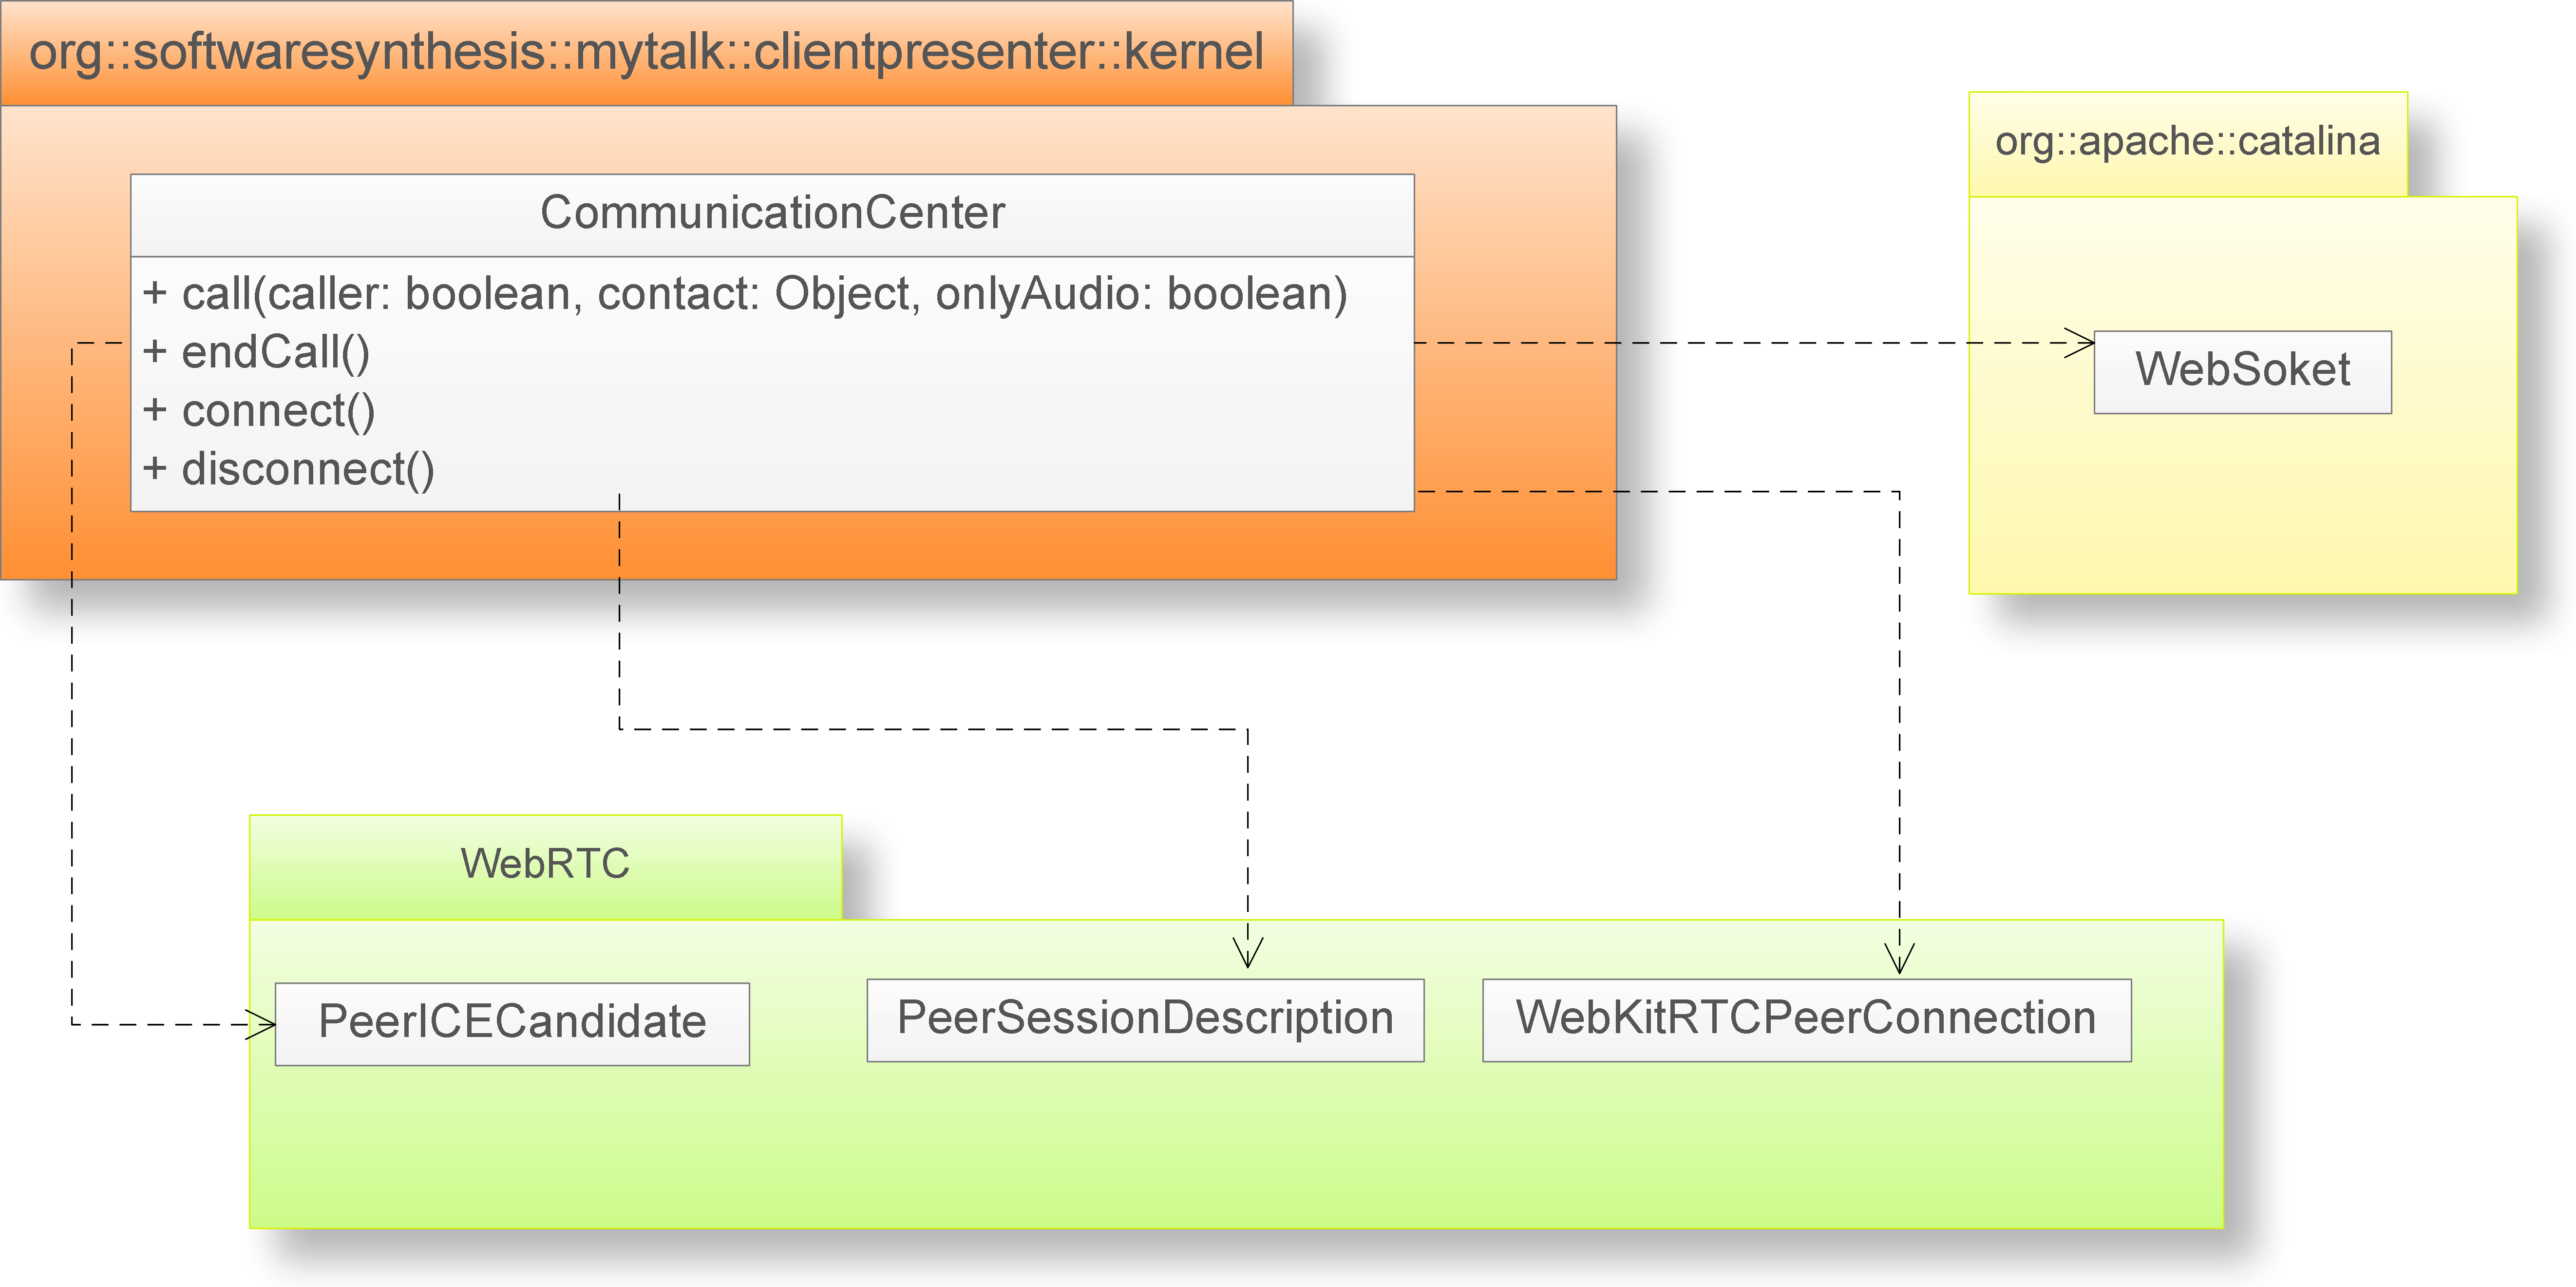
\includegraphics[width=\textwidth]{DDPKernel}
\caption{Diagramma package clientpresenter.kernel}
\end{figure}
\end{center}

\classsection{CommunicationCenter}

\subsubsection*{Funzione}
Classe logica che ha il compito di gestire tutta la parte della comunicazione lato \textit{client}.

\subsubsection*{Relazioni d'uso}
\begin{itemize}
  \item \texttt{clientpresenter.guicontrol.PresenterMediator}: utilizzato per gestire l'interazione fra il sottosistema di comunicazione e il componente di controllo dell'interfaccia grafica.
\end{itemize}

\subsubsection*{Classi estese ed interfacce implementate}
Nessuna relazione evidenziata.

\subsubsection*{Attributi}
\begin{description}
  \item{\memberdata{-- my: Object}}\\
  Mappa associativa  che contiene i dati personali dell'utente associato al client.

  \item{\memberdata{-- websocket: Object}}\\
  Oggetto WebSocket da utilizzare per lo scambio di messaggi con il server.

  \item{\memberdata{-- pc: Object}}\\
  Oggetto che rappresenta la RTCPeerConnection aperta con un altro client nel momento in cui è attiva una comunicazione audio o audio/video.
  
  \item{\memberdata{-- remoteDescriptionPacket: Array}}\\
  Array in cui viene memorizzata la descrizione del \inglese{peer} chiamante nel caso della ricezione di un messaggio di tipo 2.
  
  \item{\memberdata{-- sdpPacket: Array}}\\
  Array in cui sono memorizzati i dati relativi al \inglese{Session Description Protocol} per la descrizione dei parametri di inizializzazione delle sessioni di scambio di \inglese{stream} multimediali.
  
  \item{\memberdata{-- timer: Object}}\\
  Oggetto restituito dalla funzione \verb'setInterval' che viene creato all'avvio del \inglese{timer} per tenere traccia della durata della comunicazione in corso.
  
  \item{\memberdata{-- statCollector: Object}}\\
  Oggetto restituito dalla funzione \verb'setInterval' che viene creato all'avvio di una comunicazione al fine di tenere traccia delle statistiche che la riguardano.

\end{description}

\subsubsection*{Metodi}
\begin{description}

  \item{\method{+ call(isCaller: Boolean, contact: Object): void}}\\
  Metodo che gestisce la chiamata tramite WebRTC\@. In un primo momento si inizializza la variabile \memberdata{pc} che è di tipo RTCPeerConnection, oggetto reso disponibile dalle librerie di WebRTC dopo aver sollevato un evento \verb'chageMyState' e averne impostato la proprietà \verb'state' alla stringa \verb'"occupied"'.
  
  Successivamente dovranno essere definiti i comportamenti della RTCPeerConnection, vale a dire:
  \begin{itemize}
    \item[--] \texttt{onicecandidate}: gestore di evento che viene richiamato quando un nuovo \inglese{peer} si ``candida'' per poter chiamare, viene quindi inviata la propria descrizione all'altro \inglese{peer} tramite il server, inviando sulla \memberdata{websocket} un messaggio di tipo 2.
    
    \item[--] \texttt{onaddstream}: gestore di evento che viene richiamato quando viene aggiunto uno \textit{stream} nell'oggetto RTCPeerConnection. In questa situazione, il chiamato riceve lo \textit{stream} del chiamante e lo visualizza nell'apposito elemento \verb'<video>'. In contemporanea, vengono richiamati i metodi che fanno partire il timer della comunicazione e la visualizzazione delle statistiche di chiamata.
    
    \item[--] \texttt{onremovestream}: gestore di evento che viene richiamato quando viene rimosso uno \textit{stream} nell'oggetto RTCPeerConnection. In tal caso dovrà essere sollevato un evento \verb'changeMyState' dopo averne impostato la proprietà \verb'state' a \verb'"available"', fermare lo \inglese{stream} con il metodo \verb'stop()', chiudere la RTCPeerConnection, arrestare i timer e la visualizzazione delle statistiche e riconfigurare gli attributi \verb'src' degli elementi \verb'<video>' nel pannello della comunicazione.
  \end{itemize}

  \item{\method{+ connect(): void}}\\
  Metodo utilizzato per la creazione della connessione WebSocket con il server. A tal fine viene inizializzato il campo dati \memberdata{websocket} richiamando il costruttore con un parametro che identifica l'URL a cui è raggiungibile il sottotipo di \verb'WebSocketServlet' in ascolto sul server.
  
  In una fase successiva viene specificato il comportamento della WebSocket per determinati eventi quali:
  \begin{itemize}
    \item[--] \texttt{onopen}: gestore di evento che viene richiamato quando la WebSocket viene aperta. In questo caso, deve essere inviato alla WebSocket un messaggio di tipo  1 con il proprio identificativo utente in modo tale da identificare univocamente il canale aperto con il server. Dovrà inoltre essere sollevato un evento identificato dalla stringa \verb'changeMyState' dopo averne impostato la proprietà \verb'state' a \verb'"available"'.
    \item[--] \texttt{onclose}: gestore di evento che viene richiamato quando la WebSocket viene chiusa per qualsiasi motivo, notificando il server di tale avvenimento.
    \item[--] \texttt{onerror}: gestore di evento che viene richiamato quando avviene un errore con la WebSocket. Tale evento verrà notificato all'utente con un messaggio d'errore che descrive l'errore e l'atteggiamento da seguire.
    \item[--] \texttt{onmessage}: tale funzione ha il compito di gestire l'evento richiamato quando giunge un messaggio dal server destinato al client. Per diversificare i messaggi ricevuti, si è deciso di rappresentare il messaggio come un array nel quale il primo elemento identifica il tipo di richiesta.
    
    È possibile individuare quattro tipi di messaggi:
    \begin{itemize}
      \item[-] tipo 2: riceve e gestisce una richiesta di chiamata, estraendo l'oggetto contenuto nella seconda posizione del messaggio in una variabile \verb'signal'.
      
      Nel caso in cui si tratti di una chiamata in arrivo (quando la variabile \memberdata{pc} è \verb'null') dovrà essere salvato il \verb'signal' nel campo dati \memberdata{remoteDescriptionPacket} oppure \memberdata{sdpPacket} a seconda del fatto che il \verb'signal' contenga o meno la descrizione del \inglese{peer} chiamante e dovrà inoltre essere visualizzato l'avviso di chiamata.
      
      Nel caso invece di una chiamata in uscita, ancora una volta a seconda del fatto che il \verb'signal' contenga o meno la descrizione del \inglese{peer} chiamante, dovrà essere creata una nuova RTCSessionDescription da associare alla RTCPeerConnection tramite il metodo di libreria \verb'setRemoteDescription' oppure, in caso negativo, creare un nuovo RTCIceCandidate da associare alla RTCPeerConnection con il metodo \verb'addIceCandidate'.

       \item[-] tipo 3: riceve una richiesta con l'identificativo del chiamante come dato. Viene memorizzato nel client in modo tale da conoscere il canale che il chiamante ha aperto con il server per future comunicazioni.
      \item[-] tipo 5: notifica il cambiamento di stato degli amici. I dati ricevuti contengono l'identificativo dell'utente in seconda posizione e il relativo nuovo stato in formato stringa in terza posizione. Dovrà, quindi essere sollevato un evento \verb'changeAddressBooksContactState' dopo averne impostato le due proprietà \verb'idUserChange' e \verb'statusUserChange'.
      \item[-] tipo 6: il messaggio denota il rifiuto di una chiamata che deve essere gestito sollevando un evento con stringa identificativa \verb'rejectedCall'.
      \item[-] tipo 7: il messaggio denota l'arrivo di un nuovo messaggio testuale da visualizzare nel pannello delle chat. Dovrà pertanto essere estratto il primo parametro (che corrisponde all'utente coinvolto nella chat) e il secondo parametro (che corrisponde al testo trasmesso) quindi sollevare un evento \verb'appendMessageToChat' dopo averne impostato i relativi parametri.
    \end{itemize}
  \end{itemize}
  
  \item{\method{+ disconnect(): void}}\\
  Metodo utilizzato per disconnettersi dal sistema, tale evento deve essere notificato al server tramite la WebSocket inviando un messaggio di tipo 4 al server, chiudendo la WebSocket con il metodo di libreria \verb'close()', azzerando il contenuto della variabile \memberdata{my} e impostando a \verb'null' i valori di \memberdata{pc} e \memberdata{websocket}.

  \item{\method{+ endCall(): void}}\\
  Metodo richiamato per terminare una chiamata tra due client che ha il compito innanzitutto di sollevare un evento con identificativo \verb'changeMyState' dopo averne impostato la proprietà \verb'state' ad \verb'"available"'. In seguito dovrà essere interrotto e rimosso lo \inglese{stream} associato alla RTCPeerConnection e riconfigurati gli attributi \verb'src' degli elementi \verb'<video>' del pannello per la comunicazione. Dovranno inoltre essere fermati i timer e l'aggiornamento delle statistiche e chiusa la RTCPeerConnection memorizzata nel campo dati \memberdata{pc} dopo un'attesa di 1 secondo.
  
  \item{\method{+ onAcceptCall(contact: Object, onlyAudio: boolean): void}}\\
  Questo gestore di eventi viene richiamato all'avvenuta accettazione di una chiamata in ingresso e ha pertanto il compito di invocare il metodo \method{call} messo a disposizione dalla classe con il primo parametro a \verb'false' e inoltrando i parametri \verb'contact' e \verb'onlyAudio' associati all'evento.
  
  Alla RTCPeerConnection inizializzata durante l'esecuzione di \method{call} dovranno essere inoltre associati i valori contenuti negli attributi \memberdata{remoteDescriptionPacket} e \memberdata{sdpPacket} mediante i metodi \verb'setRemoteDescription' e \verb'addIceCandidate' messi a disposizione dalla libreria WebRTC.
  
  \item{\method{+ onChangeMyState(state: String): void}}\\
  Questo gestore di eventi ha il compito di inviare al server il messaggio che denota un cambiamento di stato dell'utente associato al client. A tal fine dovrà essere creato un array enumerativo avente in prima posizione il numero \verb'5' e in seconda posizione la stringa passata come parametro.
  
  Dovrà quindi essere invocato il metodo di libreria JSON \verb'stringify' sull'array e il testo ottenuto dovrà essere spedito al server tramite un'invocazione del metodo \verb'send' dell'oggetto WebSocket.
  
  \item{\method{+ onCall(contact: Object, onlyAudio: boolean): void}}\\
  Questo gestore di eventi viene richiamato nel momento in cui si avvia una chiamata in uscita verso un altro utente, rappresentato dal secondo parametro. Il terzo parametro rappresenta invece la natura solo audio oppure audio/video della chiamata.
  
  Il gestore dell'evento ha il compito di richiamare il metodo \method{call} messo a disposizione da questa classe con i parametri corretti (in particolare, il primo parametro dovrà essere \verb'true' dal momento che si tratta di una chiamata in uscita). Al fine di permettere la visualizzazione del pannello per l'amministrazione della chiamata dovrà essere sollevato inoltre un evento \verb'showCommunicationPanel'. Per avvisare l'utente dell'avvio della chiamata dovrà inoltre essere sollevato un evento \verb'startRinging', dopo averne impostato correttamente la proprietà \verb'evento' alla stringa \verb'"outcome"'.
  
  \item{\method{+ onRejectCall(caller: Object): void}}\\
  Questo gestore di eventi è richiamato nel momento in cui il client rifiuta una chiamata in ingresso proveniente da un altro client. A tal fine dovrà essere creato un messaggio nella forma di un array enumerativo la cui prima posizione è occupata dal valore \verb'6' e la seconda posizione dall'identificativo del chiamante. Tale messaggio, convertito in stringa tramite la funzione \verb'JSON.stringify' dovrà essere inviato al server tramite la WebSocket rappresentata dall'attributo \memberdata{websocket}.
  
  \item{\method{+ onRejectedCall(): void}}\\
  Questo gestore di evento deve essere richiamato nel momento in cui da parte dell'altro \inglese{peer} coinvolto in una chiamata in uscita giunge un rifiuto della chiamata. Al suo interno dovrà pertanto essere cambiato lo stato dell'utente sollevando un evento \verb'changeMyState' dopo averne impostato la proprietà \verb'state' alla stringa \verb'"available"'.
  
  Dovrà inoltre essere fermata la suoneria sollevando un evento \verb'stopRinging', chiusa la RTCPeerConnection e rimossi dall'interfaccia utente gli \inglese{stream} video relativi alla comunicazione.
  
  \item{\method{+ onSendMessage(contact: Object, messageText: String): void}}\\
  Questo gestore di eventi ha il compito di provocare l'invio di un messaggio testuale (corrispondente al secondo parametro) in una chat con l'utente passato come primo parametro.
  
  A tal fine dovrà essere creato un nuovo array enumerativo avente in prima posizione il numero 7, in seconda posizione l'identificativo del contatto ricevuto come primo parametro e in terza posizione il messaggio da aggiungere. Il messggio, ottenuto invocando la funzione \verb'stringify' sull'array, dovrà quindi essere inviato sulla WebSocket aperta con il server.
  
  Per visualizzare il nuovo messaggio nell'interfaccia grafica, dovrà inoltre essere sollevato un evento \verb'appendMessageToChat' dopo averne impostato le proprietà \verb'user' e \verb'text' in base ai parametri ricevuto e la proprietà \verb'amISender', ovviamente, a \verb'true' (dato che si tratta di un messaggio testuale in uscita).
  
  \item{\method{+ refusedCall(): void}}\\
  Metodo richiamato al rifiuto di una chiamata da parte dell'altro utente coinvolto in una comunicazione in uscita. Al fine di gestire questa eventualità, il metodo dovrà invocare \verb'localStream.stop()' e impostare alla stringa vuota gli attributi \verb'src' degli elementi \verb'<video>' presenti nella \classname{CommunicationView}, quindi invocate il metodo \verb'close()' sul campo dati \memberdata{pc}.

  \item{\method{+ webkitGetUserMedia(audio: Boolean, video: Boolean): void}}\\
  Metodo richiamato nel momento in cui un utente vuole iniziare una chiamata. Il metodo, fornito dalle librerie native di \underline{Chrome}, cattura lo \textit{stream} della propria videocamera/microfono. Riceve due parametri che indicano se deve essere catturato audio e/o video. Procedendo, viene aggiunto lo \textit{stream} all'oggetto RTCPeerConnection tramite il metodo \verb'addStream(localstream)' fornito dalle librerie di WebRTC\@.

% FIXME questo dovrà essere sicuramente cambiato!!
  \item{\method{-- dumpStats(obj: Object): void}}\\
  Metodo che permette l'estrazione dei dati rappresentanti le statistiche della chiamata, esso riceve come parametro un oggetto, lo elabora, ed estrae solo i byte ricevuti e inviati. Ricavati questi dati, li visualizza nello \verb'<span>' corrispondente tramite il sistema di controllo dell'interfaccia grafica del sistema.

  \item{\method{-- formatBytes(bytes: Number): String}}\\
  Metodo che formatta i byte ricevuti ed inviati al fine di fornire una visualizzazione delle statistiche in formato facilmente \inglese{human readable}.
  
Il metodo riceve come parametro un numero che rappresenta i byte e li converte in una misura espressa in KB o MB a seconda della grandezza.

  \item{\method{-- formatTime(time: Number): String}}\\
  Metodo che ritorna nel formato ``hh:mm:ss'' il tempo della comunicazione. Il metodo riceve come parametro un numero che rappresenta il tempo espresso in secondi, lo converte nel formalismo sopra descritto e quindi lo restituisce al chiamante.

  \item{\method{-- gotDescription(): void}}\\
  Metodo utilizzato da WebRTC che imposta la propria descrizione e la invia al client chiamato in modo tale da poter instaurare la comunicazione. Al suo interno dovrà quindi prima di tutto essere utilizzata la funzione della libreria di WebRTC \verb'setLocalDescription' per impostare la propria descrizione e successivamente, mediante la WebSocket aperta con il server, quest'ultima dovrà essere fatta pervenire al client \inglese{peer} chiamato.

  \item{\method{-- stopStats(): void}}\\
  Metodo che ferma l'aggiornamento delle statistiche relative alla chiamata in corso agendo sul campo dati privato \memberdata{statCollector} e che viene pertanto richiamato quando la chiamata termina

  \item{\method{-- stopTimer(): void}}\\
  Metodo che ferma l'aggiornamento del timer agendo sul campo dati privato \memberdata{time} e che deve essere richiamato quando la chiamata in corso termina.

\end{description}

\clearpage

\section{Specifica sotto-architettura \texttt{clientview}}\label{sec:clientviewarchitecture}
Il sistema dispone di dodici viste, ognuna associata ad uno specifico \inglese{presenter}. Tali viste vengono create e modificate da parte dei relativi \inglese{presenter} invocando i metodi che le viste rendono disponibili tramite la loro API pubblica.

La descrizione di ciascuna vista riportata nel presente documento comprende, oltre alla funzione, agli attributi e ai metodi che essa mette a disposizione del relativo \inglese{presenter}, anche la struttura degli elementi che la compongono.

\subsection{Package \texttt{org.softwaresynthesis.mytalk.clientview}}

\begin{center}
\begin{figure}[H]
  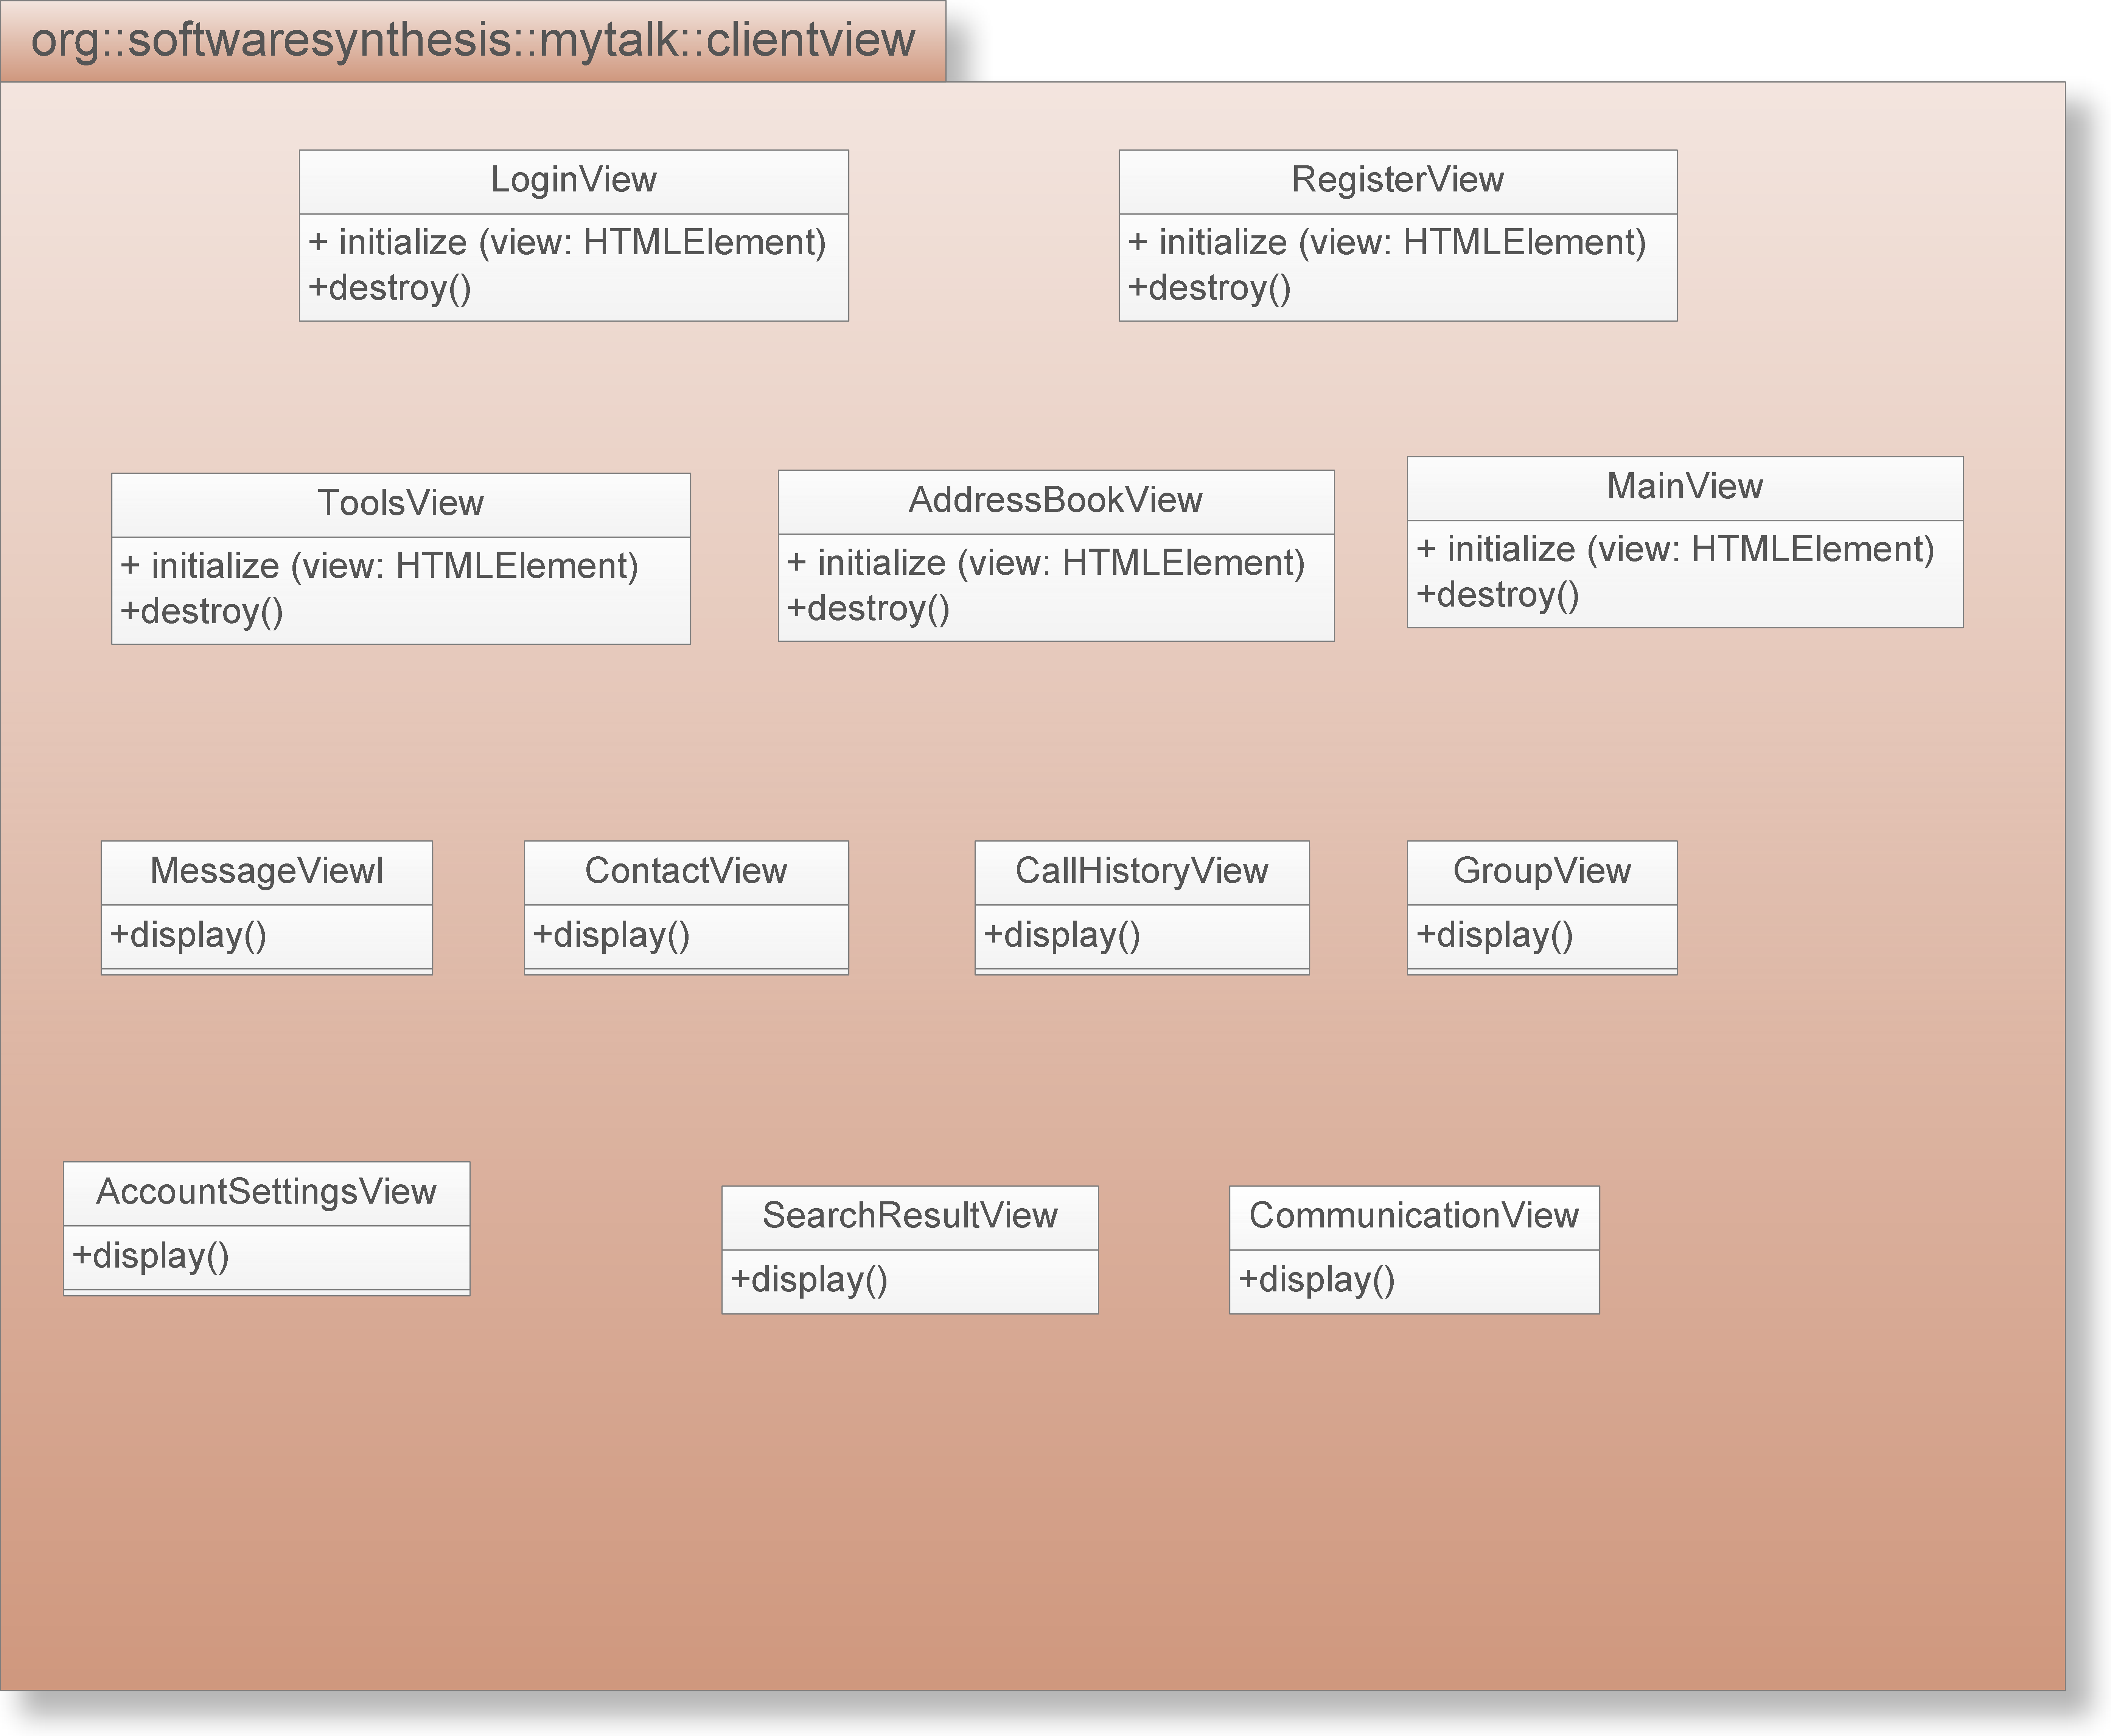
\includegraphics[width=\textwidth]{DDPClientGui}
\caption{Diagramma package clientpresenter.clientview}
\end{figure}
\end{center}

\classsection{AccountSettingsView}
\subsubsection*{Funzione}
Vista associata al \inglese{presenter} \classname{AccountSettingsPresenter} che ha il compito di permettere la visualizzazione e la modifica dei dati dell'utente.

\subsubsection*{Relazioni d'uso}
\begin{itemize}
  \item \texttt{clientpresenter.guicontrol.AccountSettingsPresenter}: per riferire il \inglese{presenter} a cui saranno inoltrati i comandi recepiti dall'interfaccia utente.
\end{itemize}

\subsubsection*{Attributi}
\begin{description}
  \item{\memberdata{-- thisPresenter: Object}}\\
  Riferimento al \inglese{presenter} associato alla vista al quale vengono inoltrati i comandi relativi alla logica applicativa tramite i gestori di eventi associati agli elementi grafici del pannello.
\end{description}

\subsubsection*{Metodi}
\begin{description}
\item{\method{+ display(): void}}\\
Tale metodo ha il compito di inizializzare la vista, ovvero l'insieme dei \inglese{widget} grafici che costituiscono il pannello per la visualizzazione delle impostazioni e dei dati dell'utente.

In particolare, la vista ha il compito di ottenere i dati relativi a nome, cognome e immagine del profilo dell'utente e popolare le apposite regioni del pannello con le informazioni corrispondenti, quindi configurare il comportamento del pulsante per la modifica dei dati alla cui pressione deve corrispondere un'invocazione del metodo \method{onChangeButtonPressed()}.

\item{\method{+ onChangeButtonPressed(): void}}\\
Gestisce la pressione del pulsante ``Modifica dati'' trasformando l'elemento \verb'<div>' che contiene l'immagine del profilo e la lista di elementi testuali in un \textit{form} da compilare per apportare i cambiamenti i propri dati di registrazione. È importante che quest'ultimo abbia per l'attributo \verb'enctype' il valore \verb'multipart/form-data'.

Il \inglese{form} è costituito da una lista i cui tre elementi \verb'<li>' contengono rispettivamente:
\begin{itemize}
  \item[--] una \verb'<label>' e il relativo campo \verb'<input>' per il nome, che inizialmente visualizza il nome precedentemente impostato nel client;
  \item[--] una \verb'<label>' e il relativo campo \verb'<input>' per il cognome dell'utente, che inizialmente visualizza il valore precedentemente impostato nel client;
  \item[--] una \verb'<label>' e il relativo campo \verb'<input>' per l'immagine del profilo (quest'ultimo dovrà avere l'attributo \verb'type' uguale a \verb'file').
\end{itemize}

Inoltre, il \inglese{form} presenta un pulsante per l'invio dei dati inseriti al server alla cui pressione deve essere attivato un gestore di evento che raccoglie i dati inseriti e li trasmette invocando il metodo \method{sendUserData} del \inglese{presenter} e quindi solleva un evento con identificativo \verb'showAccountSettingPanel' per ricaricare il pannello.

\end{description}

\subsubsection*{Elementi}
Il pannello è costituito da un elemento \verb'<div>' con identificativo uguale a \verb'AccountSettingsPanel' che contiene al proprio interno:
\begin{itemize}
  \item[--] un \verb'<div>' con attributo \verb'class' uguale a \verb'panelHeader' con all'interno un elemento \verb'<h1>' avente come figlio il solo nodo testo \textsc{<<dati personali>>};
  \item[--] un elemento \verb'<img>' con identificativo uguale alla stringa \verb'picture';
  \item[--] un elemento \verb'<ul>' contenente:
  \begin{itemize}
    \item[-] un \verb'<li>' con identificativo uguale a \verb'name';
    \item[-] un \verb'<li>' con identificativo uguale a \verb'surname';
  \end{itemize}
  \item[--] un elemento \verb'<button>' contenente il testo ``Modifica dati''.
\end{itemize}


\classsection{AddressBookView}
\subsubsection*{Funzione}
Vista associata ad \classname{AddressBookPresenter} usata per la visualizzazione della rubrica personale.

\subsubsection*{Relazioni d'uso}
\begin{itemize}
  \item \texttt{clientpresenter.guicontrol.AddressBookPresenter}: per riferire il \inglese{presenter} a cui saranno inoltrati i comandi recepiti dall'interfaccia utente.
\end{itemize}

\subsubsection*{Attributi}
\begin{description}
\item{\memberdata{-- thisPresenter: Object}}\\
Riferimento al \inglese{presenter} incaricato di controllare e aggiornare questa vista, che contiene fra i suoi metodi pubblici le funzioni di \inglese{callback} da attivare in seguito all'interazione dell'utente con i \inglese{widget} grafici contenuti nel pannello.
\end{description}

\subsubsection*{Metodi}
\begin{description}

\item{\method{+ destroy(): void}}\\
Il metodo dovrà determinare la completa eliminazione del pannello per la visualizzazione della rubrica dall'interfaccia grafica rimuovendo il nodo che corrisponde alla radice di tale pannello nell'albero DOM della UI\@.

\item{\method{+ initialize(view: String): void}}\\
Questo metodo ha il compito di provocare la visualizzazione del pannello della rubrica nell'interfaccia grafica, inserendo nel punto corretto dell'albero DOM della pagina l'elemento HTML la cui rappresentazione in formato stringa è ricevuta come parametro in ingresso.

Sarà responsabilità di questo metodo anche configurare il comportamento della vista, impostando le funzioni di \inglese{callback} che reagiscono all'interazione dell'utente con l'interfaccia grafica, eventualmente tramite le opportune chiamate ai metodi pubblici del \inglese{presenter} corrispondente.

In particolare, alla pressione del pulsante di ricerca (con identificativo \verb'inputButton') dovrà essere recuperato il valore inserito nel campo \verb'<input>' di ricerca, dovrà essere recuperato l'insieme di contatti che soddisfano il criterio di ricerca tramite un'invocazione del metodo \method{applyFilterByString} messo a disposizione dal \inglese{presenter}.

Inoltre, al verificarsi dell'evento predefinito \verb'change' associato all'elemento  \verb'<select>' (con l'identificativo \verb'selectGroup') che contiene come opzioni i gruppi della rubrica, dovranno essere effettuate le seguenti operazioni
\begin{itemize}
  \item[--] estrarre l'indice che corrisponde al gruppo selezionato accedendo alla proprietà \verb'value' dell'opzione selezionata (che avrà indice uguale al valore della proprietà \verb'selectedIndex' dell'elemento \verb'<select>');
  \item[--] calcolare l'insieme dei contatti che appartengono al gruppo mediante un'invocazione del metodo \method{applyFilterByGroup} messo a disposizione dal \inglese{presenter};
  \item[--] determinare se il gruppo è la \inglese{whitelist} in base al nome del gruppo, quindi determinare la visualizzazione del gruppo con il metodo privato \method{showFilter} della vista stessa.
\end{itemize}

\item{\method{+ initializeContactList(): void}}\\
Il compito di questo metodo è azzerare il contenuto dell'elenco di contatti visualizzato nella lista presente all'interno all'interno del pannello della rubrica, prima di un aggiornamento di quest'ultima da parte del \inglese{presenter}.

\item{\method{+ initializeGroupSelect(): void}}\\
Questo metodo ha il compito di azzerare il contenuto dell'elemento \verb'<select>' per la visualizzazione dei gruppi presente all'interno del pannello della rubrica, prima di un aggiornamento di quest'ultimo.

\item{\method{+ setState(contact: Object, state: String): void}}\\
Il metodo ha il compito di aggiornare la visualizzazione del contatto passato come primo parametro quando quest'ultimo cambia stato. Dovrà pertanto ottenere un riferimento al \inglese{list item} corrispondente, estrarne il secondo figlio che corrisponde all'immagine di stato e quindi impostarne l'attributo \verb'src' sulla base del valore calcolato dal metodo \method{getImageSrc}.

\item{\method{-- addOptionToSelect(select: HTMLElement, value: Number, text: String): void}}\\
Tale metodo di utilità ha il compito di creare una nuova opzione da visualizzare all'interno dell'elemento \verb'<select>' passato come primo parametro, che servirà per la visualizzazione dei gruppi presenti in rubrica.

Il metodo dovrà quindi creare un nuovo elemento \verb'<option>', impostarne l'attributo \verb'value' all'identificativo intero ricevuto come secondo parametro e impostarne il testo che corrisponde al nome del gruppo passato come terzo parametro. Nel caso in cui quest'ultimo valore fosse la stringa ``addrBookEntry'' -- che rappresenta la \inglese{whitelist} -- il nodo di testo da inserire nella \verb'<option>' dovrà essere la stringa ``Rubrica''.

\item{\method{-- addListItem(contact: Object): void}}\\
Il metodo ha il compito di aggiungere una nuova voce all'elenco dei contatti visualizzato nel pannello della rubrica. Dovrà pertanto ottenere prima di tutto un riferimento all'elemento \verb'<ul>' presente nel pannello, in base all'identificativo \verb'AddressBookList' che lo caratterizza.

In seguito dovrà essere creato il nuovo \verb'<li>' assegnando ad esso un identificativo uguale a quello del contatto passato come parametro. Il nuovo elemento \verb'<li>' dovrà contenere come figli
\begin{itemize}
  \item[--] un elemento \verb'<img>' per visualizzare l'immagine del contatto, con l'attributo \verb'src' uguale a \verb'contact.picturePath';
  \item[--] un nodo di testo contenente il nome del contatto (se specificato) oppure l'indirizzo email dello stesso;
  \item[--] un elemento \verb'<img>' per rappresentare lo stato del contatto, il cui attributo \verb'src' dovrà essere calcolato mediante una chiamata al metodo \method{getImageSrc}.
\end{itemize}

Inoltre, al clic dell'utente sulla nuova voce dell'elenco che rappresenta la rubrica, dovrà essere sollevato un evento avente come nome identificativo la stringa \verb'showContactPanel', dopo aver assegnato alla proprietà \verb'contact' del nuovo evento il riferimento al contatto che è visualizzato da questo metodo.

\item{\method{-- getImageSrc(contact: Object): String}}\\
Tale metodo ha il compito di restituire il percorso (relativo) corretto per l'immagine che rappresenta lo stato del contatto passato come parametro. In particolare, il metodo dovrà verificare il valore della proprietà \verb'contact.state' e restituire:
\begin{itemize}
  \item[--] il percorso \verb'img/stateavailable.png' nel caso in cui il contatto sia disponibile;
  \item[--] il percorso \verb'img/stateoccupied.png' nel caso in cui il contatto sia non disponibile o impegnato in un'altra conversazione;
  \item[--] il percorso \verb'img/stateoffline' nel caso in cui il contatto sia non in linea.
\end{itemize}

\item{\method{-- getIndexOnSelect(select:  HTMLElement, idGroup: Number): Number}}\\
Il metodo riceve come primo parametro un elemento \verb'<select>' contenente al proprio interno una serie di opzioni che rappresentano i gruppi presenti nella rubrica dell'utente. Il valore intero restituito dovrà essere l'indice dell'opzione il cui attributo \verb'value' è uguale all'identificativo del gruppo ricevuto come secondo parametro.

Tale risultato dovrà essere ottenuto iterando sulle opzioni del menu di scelta multipla grazie alla proprietà \verb'options' degli elementi \verb'<select>' resa disponibile dalle API JavaScript per la manipolazione del DOM\@.

\item{\method{-- showFilter(filteredContacts: Object, isDefaultGroup: Boolean): void}}\\
Questo metodo ha il compito di visualizzare l'insieme dei contatti passato come primo parametro in ingresso (che dovrà avere una struttura analoga a quella a quella dell'attributo \memberdata{contacts}) nella lista presente all'interno del pannello della rubrica. Il secondo parametro, invece, indica se l'insieme dei contatti passato corrisponde alla \inglese{whitlist} dell'utente.

In primo luogo, dovrà essere determinato se il metodo è invocato per visualizzare l'intera rubrica o solo una sua parte, in base al valore di \verb'idDefaultGroup' e, in caso affermativo, aggiungere un \verb'<li>' alla lista contenente il testo ``Filtraggio''. All'evento \verb'click' associato a questa voce della lista, inoltre, dovrà essere associata una funzione anonima che rimuove il filtraggio, calcolando l'indice del gruppo di \inglese{default} e quindi invocando nuovamente \method{showFilter} con il primo parametro uguale al valore di ritorno del metodo \method{applyFilterByGroup} del \inglese{presenter} e come secondo parametro \verb'true'.

In secondo luogo, dovrà essere determinato se il gruppo da visualizzare contiene almeno un contatto, tramite la proprietà \verb'length' dell'oggetto passato come primo parametro e, in caso negativo, dovrà essere aggiunto alla lista un solo \verb'<li>' contenente il nodo testo ``Nessun contatto con questo criterio''.

Infine, per ognuno degli oggetti contenuti in \verb'filteredContacts' dovrà essere invocato il metodo privato \method{addListItem} della vista, al fine di visualizzare al termine del \inglese{loop} tutti i contatti dell'insieme, come desiderato.

\end{description}

\subsubsection*{Elementi}
Il pannello è costituito da un elemento \verb'<div>' con l'identificativo \verb'LoginPanel', il quale contiene al proprio interno:
\begin{itemize}
  \item[--] un \verb'<div>' con attributo \verb'class' uguale a \verb'panelHeader' contenente un \verb'<h1>' con il solo nodo testo \textsc{<<rubrica>>} per il titolo del pannello;
  \item[--] un \verb'<div>' con l'identificativo \verb'divFilter' contenente:
  \begin{itemize}
    \item[-] un \verb'<input>' con l'identificativo \verb'inputText';
    \item[-] un \verb'<input>' di tipo \verb'image' con l'identificativo \verb'inputButton' e percorso sorgente uguale a \verb'img/search.png';
  \end{itemize}
  \item[--] un \verb'<div>' con identificativo uguale a \verb'divList' contenente a sua volta un \verb'<ul>' con l'identificativo \verb'AddressBookList';
  \item[--] un \verb'<div>' con l'identificativo \verb'divGroup' con all'interno un elemento \verb'<select>' con identificativo uguale a \verb'selectGroup';
\end{itemize}


\classsection{CallHistoryView}
\subsubsection*{Funzione}
Vista associata al \inglese{presenter} \classname{CallHistoryPresenter} utilizzata per la visualizzazione dello storico chiamate di un utente del sistema.

\subsubsection*{Relazioni d'uso}
\begin{itemize}
  \item \texttt{clientpresenter.guicontrol.CallHistoryPresenter}: per riferire il \inglese{presenter} a cui saranno inoltrati i comandi recepiti dall'interfaccia utente.
\end{itemize}

\subsubsection*{Attributi}
\begin{description}
  \item{\memberdata{-- thisPresenter: Object}}\\
  Riferimento al \inglese{presenter} associato alla vista al quale vengono inoltrati i comandi relativi alla logica applicativa tramite i gestori di eventi associati agli elementi grafici del pannello.
\end{description}

\subsubsection*{Metodi}
\begin{description}

  \item{\method{+ addListItem(call: Object): void}}\\
  Metodo che aggiunge alla lista delle chiamate visualizzata nel pannello una nuova voce che corrisponde alla chiamata passata come parametro.
  
  Ogni voce della lista contiene i dati relativi alla chiamata vale a dire l'altro utente coinvolto e la data della chiamata. Dal momento che quest'ultimo potrebbe non essere presente in rubrica, il metodo dovrà procurarsi in base all'identificativo o allo \inglese{username} un riferimento all'oggetto contatto corrispondente, quindi costruire la rappresentazione del suo nome in formato testuale.
  
  Poiché a partire da questo pannello non è possibile effettuare alcuna azione, non è presente alcuna funzione di \inglese{callback} associata alle voci della lista.
  
  \item{\method{+ display(): void}}\\
  Tale metodo ha il compito di inizializzare il pannello della vista con i dati corretti popolando la lista delle chiamate in base ai dati ricevuti dal \inglese{presenter}.
  
\end{description}

\subsubsection*{Elementi}
Il pannello è costituito da un elemento \verb'<div>' avente come identificativo il valore \verb'CallHistoryPanel' il quale, a sua volta, contiene:
\begin{itemize}
  \item[--] un elemento \verb'<div>' avente attributo \verb'class' uguale al valore \verb'panelHeader' e con all'interno un elemento \verb'<h1>' contenente il titolo \textsc{<<storico chiamate>>};
  \item[--] un elemento \verb'<ul>' avente come identificativo la stringa \verb'ulHistory'.
\end{itemize}


%TODO questa sarà da rivedere a breve!
\classsection{CommunicationView}
\subsubsection*{Funzione}
Vista associata al \inglese{presenter} \classname{CommunicationPresenter} utilizzata durante una chiamata audio e per la gestione delle chat testuali con gli altri utenti.

\subsubsection*{Relazioni d'uso}
\begin{itemize}
  \item \texttt{clientpresenter.guicontrol.CommunicationPresenter}: per riferire il \inglese{presenter} a cui saranno inoltrati i comandi recepiti dall'interfaccia utente.
\end{itemize}

\subsubsection*{Attributi}
\begin{description}

  \item{\memberdata{-- chatElements: Object}}\\
  Array associativo i cui valori sono costituiti da una serie di \verb'HTMLElement' che rappresentano tutte le chat aperte in un dato momento, mentre i cui valori sono gli identificativi degli utenti coinvolti nella comunicazione.

  \item{\memberdata{-- thisPresenter: Object}}\\
  Riferimento al \inglese{presenter} associato alla vista al quale vengono inoltrati i comandi relativi alla logica applicativa tramite i gestori di eventi associati agli elementi grafici del pannello.
\end{description}

\subsubsection*{Metodi}
\begin{description}

  \item{\method{+ display(): void}}\\
  Tale metodo ha il compito di inizializzare il comportamento della vista, in particolare assegnando all'evento \verb'click' del pulsante per la chiusura della chat deve essere sollevato un evento avente come nome identificativo la stringa \verb'callEnded'.

  \item{\method{+ onAppendMessage(user: Object, text: String, amISender: Boolean): void}}\\
  Questo gestore di eventi ha il compito di aggiungere la stringa passata come secondo parametro all'interno dell'area di testo che è associata alla chat con l'utente passato come primo parametro del metodo, dopo averla recuperata dall'attributo \memberdata{chatElements}.

  A seconda del fatto che il mittente del messaggio sia o meno l'utente del client, il testo del messaggio dovrà essere concatenato alla stringa \verb'"io: "' oppure \verb'contact.name + ": "'.

  \item{\method{+ onChatAdded(user: Object): void}}\\
  Questo gestore di eventi provoca l'aggiunta di una chat che coinvolge con l'utente ricevuto come parametro aggiornando il campo privato \memberdata{chatElements}. Inoltre, dovrà essere creato un nuovo elemento \verb'<li>' tramite una chiamata al metodo \method{createChatItem}, che dovrà essere aggiunto al sotto-albero radicato nell'elemento \verb'<ul>' con l'identificativo uguale a \verb'ulOpenChat'.

  \item{\method{+ onChatRemoved(user: Object): void}}\\
  Questo gestore di eventi provoca la chiusura definitiva della chat aperta con l'utente passato come parametro eliminando l'elemento corrispondente da \memberdata{chatElements} e rimuovendo contestualmente l'elemento HTML corrispondente al \verb'<li>' della chat dalla lista con identificativo \verb'ulOpenChat'.

  Inoltre, se l'utente passato come parametro è associato proprio alla chat visualizzata all'interno del pannello, quest'ultima dovrà essere eliminata anche dall'albero DOM dell'interfaccia grafica oltre che dall'attributo \memberdata{chatElements}.

  \item{\method{+ onUpdateStats(text: String, isReceivedData: Boolean): void}}\\
  Il metodo controlla tramite il parametro \verb'isReceivedData' ricevuto in input se è necessario aggiornare lo \verb'<span>' relativo ai dati inviati oppure lo \verb'<span>' relativo ai dati ricevuti e lo imposta con il valore del primo parametro dopo aver anteposto il prefisso \verb'"Dati inviati: "' oppure \verb'"Dati ricevuti: "' a seconda del caso.

  \item{\method{+ onUpdateTimer(text: String): void}}\\
  Il metodo aggiorna il tempo di comunicazione durante una chiamata. Imposta il contenuto dello \verb'<span>' relativo alla visualizzazione del tempo chiamata con il valore della stringa ricevuta come parametro in ingresso, dopo aver aggiunto il prefisso \verb'"Tempo chiamata: "'.

  \item{\method{- createChatElement(user: Object): HTMLElement}}\\
  Tale metodo restituisce un elemento HTML costituito da un \verb'<div>' che rappresenta l'area occupata dalla chat con l'utente passato come parametro. A tale elemento viene assegnato l'identificativo \verb'divContainerChat'.
  
  Deve inoltre essere aggiunto come ultimo figlio del \verb'<div>' anche un \verb'<form>' avente come identificativo la proprietà \verb'id' dell'utente passato come parametro preceduta dal prefisso \verb'"chatForm-"'. A tale \verb'<form>' dovranno essere aggiunti:
  \begin{itemize}
    \item[--] una \verb'<textarea>' con l'identificativo \verb'chatText' dove andrà visualizzata la cronologia della chat;
    \item[--] una campo di di input testuale con l'identificativo uguale \verb'input';
    \item[--] un pulsante per inviare il messaggio contenente il nodo di testo \verb'"Invia"' al cui evento \verb'click' è attivata una funzione anonima che solleva un evento \verb'sendMessage' dopo averne impostato la proprietà \verb'contact' con l'utente passato come parametro e la proprietà \verb'text' al valore estratto dall'area di testo \verb'chatText'.
  \end{itemize}

  \item{\method{-- createChatItem(user: Object): HTMLElement}}\\
  Tale metodo restituisce un elemento HTML di tipo \verb'<li>' contenente l'identificativo dell'utente che corrisponde all'oggetto passato come parametro.
  
   Al \inglese{list item} restituito viene assegnato un identificativo corrispondente a quello dell'utente con cui si vuole dialogare con il prefisso \verb'"chat-"'. All'evento \verb'click' associato a questo \verb'<li>' si collega tramite una funzione anonima un'invocazione del metodo privato \method{displayChat} con il parametro \verb'user' che fa visualizzare la chat. Viene inoltre creato un pulsante per chiudere la chat al cui evento \verb'click' è associata una funzione anonima che richiama il metodo \method{removeChat} ancora passando \verb'user' come parametro.

  \item{\method{-- displayChat(user: Object): void}}\\
  Provoca la visualizzazione della chat che coinvolge l'utente passato come parametro nell'interfaccia grafica posizionando correttamente nell'albero DOM della pagina l'elemento che può essere ottenuto da \memberdata{chatElements} in corrispondenza della chiave \verb'user.id'.

\end{description}

\subsubsection*{Elementi}
Il pannello è costituito da un \verb'<div>' con l'identificativo \verb'CommunicationPanel', il quale contiene al proprio interno:
\begin{itemize}
  \item[--] un \verb'<div>' di classe \verb'panelHeader' contenente un elemento \verb'<h1>' con il solo nodo testo \textsc{<<comunicazione>>};
  \item[--] un \verb'<div>' con l'identificativo \verb'divCall' contenente:
  \begin{itemize}
    \item[-] un elemento \verb'<video>' con l'identificativo \verb'myVideo' e gli attributi booleani \verb'autoplay' e \verb'muted' attivati;
    \item[-] un elemento \verb'<video>' con l'identificativo \verb'otherVideo' e l'attributo \verb'autoplay' attivato;
    \item[-] un \verb'<div>' con l'identificativo \verb'statDiv' contenente:
    \begin{itemize}
      \item[$\cdot$] uno \verb'<span>' con l'identificativo \verb'statSpan' con all'interno uno \verb'<span>' con l'identificativo \verb'statRecevd' e un altro \verb'<span>' con l'identificativo \verb'statSend';
      \item[$\cdot$] uno \verb'<span>' con l'identificativo \verb'timerSpan';
    \end{itemize}
    \item[-] un \verb'<button>' con identificativo \verb'closeButton' e l'etichetta ``Termina'';
  \end{itemize}
  \item[--] un \verb'<div>' con l'identificativo \verb'divChat' con al proprio interno un elemento \verb'<ul>' con identificativo uguale a \verb'ulOpenChat'. 
\end{itemize}


\classsection{ContactView}
\subsubsection*{Funzione}
Vista associata al \inglese{presenter} \classname{ContactPresenter} utilizzata per visualizzare il profilo di un utente, gestire la sua collocazione nella rubrica e/o avviare una comunicazione con quest'ultimo.

\subsubsection*{Relazioni d'uso}
\begin{itemize}
  \item \texttt{clientpresenter.guicontrol.ContactPresenter}: per riferire il \inglese{presenter} a cui saranno inoltrati i comandi recepiti dall'interfaccia utente.
\end{itemize}

\subsubsection*{Attributi}
\begin{description}
  \item{\memberdata{-- thisPresenter: Object}}\\
  Riferimento al \inglese{presenter} associato alla vista al quale vengono inoltrati i comandi relativi alla logica applicativa tramite i gestori di eventi associati agli elementi grafici del pannello.
\end{description}

\subsubsection*{Metodi}
\begin{description}

  \item{\method{+ display(): void}}\\
  Il metodo dovrà innanzitutto visualizzare l'insieme dei dati personali che costituiscono il profilo del contatto selezionato, che corrisponde al valore dell'attributo \memberdata{currentContact}. Dovranno pertanto essere effettuate le seguenti operazioni
  \begin{itemize}
    \item[--] recuperare un riferimento al \verb'<li>' per la visualizzazione del nome, tramite il suo identificativo (\verb'contactName') e aggiungere ad esso un nodo di testo ottenuto come \verb'"Nome: " currentContact.name';
    \item[--] recuperare un riferimento al \verb'<li>' per la visualizzazione del cognome, tramite il suo identificativo (\verb'contactSurname') e aggiungere ad esso un nodo di testo ottenuto come \verb'"Cognome: " currentContact.surname';
    \item[--] recuperare un riferimento al \verb'<li>' per la visualizzazione dell'indirizzo email, tramite il suo identificativo (\verb'contactEmail') e aggiungere ad esso un nodo di testo ottenuto come \verb'"Email: " currentContact.email';
    \item[--] recuperare un riferimento all'elemento \verb'<img>' (con identificativo \verb'contactAvatar') per la visualizzazione dell'immagine del profilo e impostarne l'attributo \verb'src' uguale al valore di \verb'currentContct.picturePath'.
  \end{itemize}
  
  In un secondo momento dovrà essere impostata correttamente la visualizzazione dei pulsanti di blocco/sblocco e dell'eventuale stato di blocco del contatto tramite il metodo \method{adjustBlockButtonDisplay}, quindi visualizzare i pulsanti corretti per interagire con il contatto a seconda dello stato, tramite il metodo \method{adjustGUIOnContactState}.
  
  In terzo luogo, dovrà essere visualizzato correttamente il sotto-pannello per la gestione dei gruppi cui il contatto appartiene, mediante una chiamata al metodo \method{buildGroupsDiv}.
  
  Infine dovrà essere configurato il comportamento dei pulsanti presenti nel pannello, in particolare:
  \begin{itemize}
    \item[--] alla pressione del pulsante per aggiungere il contatto alla rubrica dovrà essere sollevato un evento con identificativo \verb'addContactToAddressBook' dopo averne impostato la proprietà \verb'contact' uguale a \memberdata{currentContact};
    \item[--] alla pressione del pulsante per la rimozione del contatto alla rubrica dovrà essere sollevato un evento con identificativo \verb'removeContactToAddressBook' dopo averne impostato la proprietà \verb'contact' uguale a \memberdata{currentContact};
    \item[--] alla pressione del pulsante per bloccare il contatto dovrà essere sollevato un evento con identificativo \verb'blockContact' dopo averne impostato la proprietà \verb'contact' uguale a \memberdata{currentContact}, quindi dovrà essere aggiornato il pannello sollevando un evento con identificativo \verb'showContactPanel' dopo averne impostato la proprietà \verb'contact';
    \item[--] alla pressione del pulsante per sbloccare il contatto dovrà essere sollevato un evento con identificativo \verb'unlockContact' dopo averne impostato la proprietà \verb'contact' uguale a \memberdata{currentContact}, quindi dovrà essere aggiornato il pannello sollevando un evento con identificativo \verb'showContactPanel' dopo averne impostato la proprietà \verb'contact';
    \item[--] alla pressione del pulsante per avviare una comunicazione audio con il contatto dovrà essere sollevato un evento con l'identificativo \verb'call' dopo averne impostato la proprietà \verb'contact' col valore di \memberdata{currentContact} e la proprietà \verb'isOnlyAudio' a \verb'false';
    \item[--] alla pressione del pulsante per avviare una comunicazione audio/video con il contatto dovrà essere sollevato un evento con l'identificativo \verb'call' dopo averne impostato la proprietà \verb'contact' col valore di \memberdata{currentContact} e la proprietà \verb'onlyAudio' a \verb'true';
    \item[--] alla pressione del pulsante per avviare una chat testuale con il contatto dovrà essere sollevato un evento con l'identificativo \verb'chatStarted' dopo averne impostato la proprietà \verb'user' col valore di \memberdata{currentContact};
    \item[--] alla pressione del pulsante per lasciare un messaggio nella segreteria del contatto dovrà essere sollevato un evento con identificativo uguale a \verb'showPhoneCallMessagePanel', dopo averne impostato la proprietà \verb'contact' uguale al valore di \memberdata{currentContact}.
  \end{itemize}
  
  Infine, nel caso in cui il contatto dovesse essere già presente nella rubrica, dovrà essere impedita la visualizzazione del pulsante per aggiungerlo alla rubrica, impostando la proprietà \verb'style.display' al valore \verb'"none"'.

  \item{\method{-- adjustBlockButtonDisplay(contact: Object): void}}\\
  Il metodo avrà il compito di impostare la corretta visualizzazione dell'elemento \verb'<div>' contenente le informazioni relative al blocco del contatto e la visualizzazione del \verb'<button>' per bloccare e del \verb'<button>' per sbloccare il contatto in ragione dello stato (bloccato o meno) in cui si trova lo stesso.
  
  In particolare, se il contatto è bloccato, la proprietà \verb'style.display' dei tre elementi dovrà essere, rispettivamente, \verb'"block"', \verb'"none"' e \verb'"inline"'. Se invece il contatto non è bloccato, allora le proprietà di stile dovranno essere rispettivamente impostate a \verb'"none"', \verb'"inline"' e \verb'"none"'.
  
  \item{\method{-- adjustGUIOnContactState(contact: Object): void}}\\
  Questo metodo avrà il compito di configurare i pulsanti che permettono di avviare una comunicazione (audio, audio/video o testuale) e di lasciare un messaggio in segreteria sulla base del contatto passato come parametro.
  
  In dettaglio, se il contatto è \inglese{online} e pertanto disponibile ad accettare comunicazioni in ingresso la proprietà \verb'style.display' dei pulsanti corrispondenti alle tre comunicazioni dovranno essere impostate a \verb'"inline"' mentre il pulsante per attivare la segreteria dovrà essere nascosto impostando detta proprietà a \verb'"none"'. Dualmente, se il contatto è invece \inglese{offline} le proprietà dei pulsanti per le comunicazioni dovranno essere \verb'"none"' e quella del pulsante della segreteria sarà invece \verb'"inline"'.
  
  \item{\method{-- buildGroupsDiv(contact: Object): void}}\\
  Lo scopo di questo metodo è popolare l'elemento \verb'<div>' che visualizza i gruppi della rubrica cui appartiene il contatto e permette di effettuare alcune operazioni di amministrazione della rubrica (la rimozione del contatto da un gruppo).
  
  Il metodo dovrà pertanto recuperare innanzitutto l'insieme di tutti i gruppi tali che il \memberdata{currentContact} vi appartiene, invocando il metodo \method{getGroupsWhereContactIs} messo a disposizione da \classname{PresenterMediator}.
  
  Per ognuno di questi gruppi dovrà essere creato un elemento \verb'<span>' con attributo \verb'class' uguale a \verb'groupLabel', il quale dovrà contenere al proprio interno un nodo di testo con il nome del gruppo e un elemento \verb'<img>' con percorso uguale a \verb'img/close.png' e classe \verb'deleteGroupButton', al cui evento \verb'click' dovrà essere sollevato un evento con identificativo \verb'removeContactFromGroup', dopo averne impostato le proprietà \verb'contact' e \verb'group' in funzione del contatto visualizzato e del gruppo su cui si sta iterando.
  
\end{description}

\subsubsection*{Elementi}
Il pannello è costituito da un elemento \verb'<div>' con l'identificativo \verb'ContactPanel', che contiene:
\begin{itemize}
  \item[--] un \verb'<div>' con classe uguale a \verb'panelHeader' contenente un \verb'<h1>' con all'interno il solo nodo di testo \textsc{<<scheda contatto>>};
  \item[--] un \verb'<div>' con l'identificativo \verb'displayBlockedDiv' contenente il testo ``Contatto bloccato'';
  \item[--] un elemento \verb'<img>' per visualizzare l'immagine del profilo;
  \item[--] una \verb'<ul>' per la  visualizzazione dei dati personali del contatto, contenente al suo interno:
  \begin{itemize}
    \item[-] un \verb'<li>' con l'identificativo \verb'contactName';
    \item[-] un \verb'<li>' con l'identificativo \verb'contactSurname';
    \item[-] un \verb'<li>' con l'identificativo \verb'contactEmail';
  \end{itemize}
  \item[--] un elemento \verb'<div>' con l'identificativo \verb'groupsDiv';
  \item[--] un \verb'<div>' con l'identificativo \verb'buttonsDiv' contenente al suo interno:
  \begin{itemize}
    \item[-] un elemento \verb'<button>' con l'identificativo \verb'callButton' e l'etichetta ``Chiama'';
    \item[-] un \verb'<button>' con l'identificativo \verb'videoCallButton' e l'etichetta ``Video-chiama'';
    \item[-] un \verb'<button>' con l'identificativo \verb'chatButton' e l'etichetta ``Avvia chat testuale'';
    \item[-] un elemento \verb'<button>' con l'identificativo \verb'messageButton' e l'etichetta ``Lascia messaggio in segreteria'';
    \item[-] un elemento \verb'<button>' con l'identificativo \verb'addToAddressBookButton' e l'etichetta ``Aggiungi in rubrica'';
    \item[-] un elemento \verb'<button>' con l'identificativo \verb'removeFromAddressBookButton' e l'etichetta ``Rimuovi dalla rubrica'';
    \item[-] un elemento \verb'<button>' con l'identificativo \verb'blockButton' e l'etichetta ``Blocca'';
    \item[-] un elemento \verb'<button>' con l'identificativo \verb'unlockButton' e l'etichetta ``Sblocca''.
  \end{itemize}
\end{itemize}


\classsection{GroupView}
\subsubsection*{Funzione}
Vista associata al \classname{GroupPresenter} utilizzata per la visualizzazione dei gruppi della rubrica.

\subsubsection*{Relazioni d'uso}
\begin{itemize}
  \item \texttt{clientpresenter.guicontrol.GroupPresenter}: per riferire il \inglese{presenter} a cui saranno inoltrati i comandi recepiti dall'interfaccia utente.
\end{itemize}

\subsubsection*{Attributi}
\begin{description}
  \item{\memberdata{-- thisPresenter: Object}}\\
  Riferimento al \inglese{presenter} associato alla vista al quale vengono inoltrati i comandi relativi alla logica applicativa tramite i gestori di eventi associati agli elementi grafici del pannello.
\end{description}

\subsubsection*{Metodi}
\begin{description}
  
  \item{\method{+ addListItem(group: Object): void}}\\
  Il metodo ha lo scopo di aggiungere una nuova voce alla lista con identificativo \verb'groupList' presente nel pannello. Ogni nuova \verb'<li>' dovrà essere a sua volta composta da:
  \begin{itemize}
    \item[--] un pulsante sotto forma di immagine per mostrare il contenuto del gruppo con l'attributo \texttt{class} uguale a \texttt{showGroupContacts} e percorso \texttt{img/expandGroupImg.png};
    \item[--] un elemento \verb'<span>' con un nodo di testo  che rappresenta il nome gruppo stesso;
    \item[--] un pulsante sotto forma di immagine con attributo \texttt{class} uguale a \texttt{deleteGroup} e percorso \texttt{img/deleteGroupImg.png} per la rimozione del gruppo;
    \item[--] un pulsante sotto forma di immagine con attributo \texttt{class} uguale a \texttt{addContactInGroup} e percorso \texttt{img/addToGroupImg.png} per l'aggiunta di un nuovo contatto all'interno del gruppo stesso;
    \item[--] un elemento \verb'<ul>' che rappresenta la lista (in forma estesa oppure compatta) dei contatti della rubrica che appartengono al gruppo in oggetto.
  \end{itemize}
  
  Il metodo dovrà inoltre associare ai tre pulsanti le funzioni di \inglese{callback} per la gestione dell'evento \verb'click', in particolare:
  \begin{itemize}
    \item[--] alla pressione del pulsante per invertire la modalità di visualizzazione del gruppo, dovrà essere cambiato l'attributo \verb'class' della lista dei contatti del gruppo da \verb'collapsedList' a \verb'uncollapsedList' (o viceversa) e, nel caso in cui il pulsante sia utilizzato per visualizzare un gruppo in forma compatta, dovrà essere rimosso il \inglese{form} mediante il quale sarà possibile aggiungere nuovi contatti al gruppo;
    \item[--] alla pressione del pulsante per aggiungere un nuovo contatto al gruppo dovrà essere impostata la visualizzazione compatta dei membri del gruppo, quindi dovrà essere creato il \inglese{form} per l'aggiunta di un nuovo contatto al gruppo utilizzando il metodo privato \method{createAddToGroupForm} della vista stessa;
    \item[--] alla pressione del pulsante per l'eliminazione di un gruppo, dovrà essere chiesta conferma all'utente con un'istruzione del tipo
    \begin{verbatim}
confirm("Sei sicuro di voler eliminare il gruppo" + group.name + "?");
    \end{verbatim}
    e, in caso di risposta affermativa, dovrà essere sollevato un evento con nome identificativo uguale a \verb'deleteGroup' (dopo averne assegnato la proprietà \verb'group') cui risponderà il \inglese{presenter} incaricato di inviare al server la richiesta corrispondente, quindi provocare l'aggiornamento del pannello sollevando un evento \verb'showGroupPanel'.
  \end{itemize}
  
  \item{\method{+ display(): void}}\\
  Il metodo ha il compito di inizializzare la vista, ovvero l'insieme dei \inglese{widget} grafici che costituiscono il pannello per la gestione dei gruppi della rubrica.
  
  In particolare, alla pressione del pulsante per l'aggiunta di un nuovo gruppo dovrà essere chiesto all'utente con una finestra di dialogo il nome del gruppo e, se il nome inserito è non vuoto,  dovrà essere sollevato un evento con stringa identificativa \verb'createGroup', dopo averne assegnato la proprietà \verb'groupName', quindi aggiornare il pannello sollevando un evento con l'identificativo \verb'showGroupPanel'.
  
  Dal momento che per popolare il pannello con i dati necessari è necessario prima scaricarli dal server, la vista invoca il metodo \method{displayGroupList()} del relativo \inglese{presenter} per portare a termine l'operazione.
  
  \item{\method{-- createAddToGroupForm(group: Object): HTMLElement}}\\
  Un'invocazione di tale metodo dovrà fare in modo che sia creato il \inglese{form} per l'aggiunta di un nuovo contatto al gruppo passato come parametro in ingresso. La vista dovrà innanzitutto ottenere un insieme dei contatti per cui è possibile l'aggiunta nel suddetto gruppo, mediante il metodo \method{selectCandidates} fornito dal \inglese{presenter} associato.
  
  In secondo luogo, dovrà essere creato un elemento \verb'<fieldset>' contenente una serie di \verb'<input>' (di tipo \verb'checkbox') e \verb'<label>' per ognuno dei contatti candidati all'aggiunta.
  
  Infine, dovranno essere aggiunti al \verb'<form>' due pulsanti, uno per determinare l'aggiunta di tutti i contatti selezionati all'interno del gruppo visualizzato e uno per terminare l'operazione di inserimento nascondendo il relativo \inglese{form}. Il metodo dovrà inoltre terminare restituendo al chiamante un riferimento all'elemento HTML \verb'<form>' appena creato.
  
  \item{\method{-- createContactList(group: Object): HTMLElement}}\\
  Questo metodo ha il compito di creare la lista dei contatti che appartengono al gruppo passato come parametro in ingresso, che dovrà avere di default il valore dell'attributo \verb'class' impostato a \verb'collapsedList'.
  
  Dovrà inoltre essere creato un nuovo elemento \verb'<ul>' all'interno del quale aggiungere un nodo \verb'<li>' per ogni contatto del gruppo. Le voci di questa lista saranno formate da un nodo di testo contenente il nome del contatto, più un pulsante sotto forma di immagine avente la classe \verb'deleteContact' e percorso uguale a \verb'img/deleteContactImg.png'.
  
  Alla pressione di questo pulsante dovrà essere sollevato un evento con identificativo \verb'removeContactFromGroup' dopo averne correttamente impostato le proprietà \verb'contact' e \verb'group' e, in seguito, dovrà essere sollevato un evento \verb'showGroupPanel' al fine di visualizzare nuovamente il pannello. La lista così costituita dovrà, infine, essere restituita al chiamante del metodo.

\end{description}

\subsubsection*{Elementi}
Il pannello è rappresentato da un elemento \verb'<div>' con identificativo uguale a \verb'GroupPanel' ed è costituito dai seguenti elementi:
\begin{itemize}
  \item[--] un \verb'<div>' con attributo \verb'class' uguale a \verb'panelHeader' con all'interno un elemento \verb'<h1>' contenente il solo nodo di testo \textsc{gestione gruppi};
  \item[--] una \verb'<ul>' con identificativo uguale a \verb'groupList'.
\end{itemize}


\classsection{LoginView}
\subsubsection*{Funzione}
Vista associata al \inglese{presenter} \classname{LoginPresenter} utilizzata per effettuare il login nel sistema.

\subsubsection*{Relazioni d'uso}
\begin{itemize}
  \item \texttt{clientpresenter.guicontrol.LoginPresenter}: per riferire il \inglese{presenter} a cui saranno inoltrati i comandi recepiti dall'interfaccia utente.
\end{itemize}

\subsubsection*{Attributi}
\begin{description}
  \item{\memberdata{-- thisPresenter: Object}}\\
  Riferimento al \inglese{presenter} associato alla vista al quale vengono inoltrati i comandi relativi alla logica applicativa tramite i gestori di eventi associati agli elementi grafici del pannello.
\end{description}

\subsubsection*{Metodi}
\begin{description}

  \item{\method{+ correctAnswer(): void}}\\
	Metodo usato per modificare il nodo DOM salvato nella variabile \memberdata{thisPanel} per comunicare all'utente che la risposta da lui inserita per il recupero \textit{password} è corretta. 
	
Il metodo deve rimuovere il figlio con identificativo uguale a \texttt{passwordretrieval} dalla vista, quindi aggiunge un nuovo elemento \verb'<p>' contenente il messaggio:
\begin{verbatim}
	Recupero password avvenuto correttamente.
	Ti è stata inviata un'email contenente i dati richiesti.
\end{verbatim}
il messaggio citato è temporaneo e dovrà essere rimosso allo scadere di un \inglese{timeout} della durata di due secondi utilizzando la funzione \verb'window.setTimeout(funtion() {...}, 2000)'.

Il corpo della funzione anonima passata a \verb'setTimeout' avrà il compito di rimuovere dall'elemento \verb'thisPanel' il paragrafo creato in precedenza.

  \item{\method{+ destroy(): void}}\\
  Tale metodo ha il compito di eliminare il pannello dall'interfaccia grafica visualizzata. A tal fine, deve essere rimosso il nodo che corrisponde al pannello nell'albero DOM della UI\@.
  
  \item{\method{+ errorLogin(): void}}\\
  Il metodo ha lo scopo di segnalare visivamente all'utente il fatto che si è verificato un errore nell'elaborazione delle credenziali di autenticazione inserite nel \inglese{form}. Tale effetto dovrà essere ottenuto aggiungendo al valore dell'attributo \verb+class+ il valore \verb+error+.

	\item{\method{+ incorrectAnswer(): void}}\\
	Metodo che in caso di inserimento della risposta non corretta alla domanda segreta visualizza un messaggio di avvertimento all'utente per due secondi quindi lascia il controllo al \inglese{form} di inserimento della risposta alla domanda segreta.
	
	Il metodo deve cercare un elemento \verb'<p>' per la visualizzazione del messaggio, contenente il seguente testo:
\begin{verbatim}
	Dati non corretti. Inserire nuovamente la risposta.
\end{verbatim}
	
	Tale messaggio dovrà essere visualizzato con una procedura analoga a quella usata in \method{correctAnswer()}.

	\item{\method{+ initialize(view: String): void}}\\
	Il metodo ha il compito di inizializzare il pannello di login dopo che è stato caricato il relativo \inglese{template} che crea di tutti i \inglese{widget} grafici contenuti al suo interno e che viene ricevuto in forma testuale come parametro in ingresso.
	
	Oltre ad aggiungere all'interfaccia grafica il sotto-albero DOM che riceve come parametro in ingresso, il metodo dovrà configurare il pannello assegnando ai pulsanti le funzioni di \inglese{callback} corrispondenti.
	
	In particolare, alla pressione del pulsante di login deve essere eseguita una funzione che recupera il nome utente e la \textit{password} inseriti dall'utente (con i metodi \method{getUsername()} e \method{getPassword()} rispettivamente), quindi invocare il metodo \method{login} del \inglese{presenter} per la valutazione dei dati.
	
	Alla pressione del pulsante di registrazione deve invece essere sollevato un evento che provoca la visualizzazione del pannello di registrazione, vale a dire un evento con stringa identificativa uguale a \verb'showRegistrationPanel'.
	
	Infine, alla pressione del pulsante per il recupero della \textit{password} deve essere costruito il \inglese{form} corrispondente, mediante una chiamata al metodo \method{buildRetrievePasswordForm()}, aggiungendo l'elemento restituito all'interfaccia grafica finale.
	
	\item{\method{-- buildRetrievePasswordForm(): HTMLElement}}\\
	Metodo usato per costruire il \inglese{form} per il recupero della \textit{password}, che ha il compito di costruire un elemento \verb'fieldset', che contiene al suo interno:
	\begin{itemize}
	  \item[--] un \verb'<label>' contenente la domanda segreta;
	  \item[--] un elemento \verb'<input>' per inserire il testo della risposta;
	  \item[--] un \verb'<input>' di tipo \verb'submit' per l'invio dei dati.
	\end{itemize}
Alla pressione di quest'ultimo, la vista dovrà invocare il metodo \method{hasAnsweredCorrectly} del \inglese{presenter} associato e, in base al risultato positivo o negativo ottenuto, visualizzare il messaggio corrispondente tramite i metodi \verb'correctAnswer()' e \verb'incorrectAnswer()' rispettivamente.

Infine, il metodo restituisce il nodo DOM radice della nuova porzione di interfaccia grafica creata, vale a dire il \verb'<fieldset>'.

\end{description}

\subsubsection*{Elementi}
Il pannello contiene un elemento \verb'<div>' con identificativo uguale a \verb'LoginPanel' il quale a sua volta ha come figlio un \verb'<fieldSet>' con identificativo uguale a \verb'loginForm' che contiene:
  \begin{itemize}
    \item[--] un elemento \verb'<div>' per il logo;
    \item[--] un elemento \verb'<ul>' contenente i seguenti elementi:
    \begin{itemize}
      \item[-] un elemento \verb'<li>' per il nome utente, con all'interno un elemento \verb'<label>' e il relativo campo di inserimento \verb'<input>';
      \item[-] un elemento \verb'<li>' per la \textit{password}, con all'interno un elemento \verb'<label>' e il relativo campo di inserimento \verb'<input>';
      \item[-] \verb'<li>' per i pulsanti contenente al suo interno:
      \begin{itemize}
        \item[$\cdot$] un elemento \verb'<button>' per effettuare il login;
        \item[$\cdot$] un elemento \verb'<button>' per effettuare la registrazione al sistema;
        \item[$\cdot$] un elemento \verb'<button>' per recuperare i dati dimenticati.
      \end{itemize}
    \end{itemize}
  \end{itemize}
  

\classsection{MainView}
\subsubsection*{Funzione}
Vista associata al \classname{MainPresenter} che contiene il pannello principale ed è responsabile del suo aggiornamento e della sua visualizzazione.

\subsubsection*{Relazioni d'uso}
\begin{itemize}
  \item \texttt{clientpresenter.guicontrol.MainPresenter}: per riferire il \inglese{presenter} a cui saranno inoltrati i comandi recepiti dall'interfaccia utente.
\end{itemize}

\subsubsection*{Attributi}
\begin{description}
  \item{\memberdata{-- thisPresenter: Object}}\\
  Riferimento al \inglese{presenter} associato alla vista al quale vengono inoltrati i comandi relativi alla logica applicativa tramite i gestori di eventi associati agli elementi grafici del pannello.
\end{description}

\subsubsection*{Metodi}
\begin{description}
  \item{\method{+ destroy(): void}}\\
  Metodo che ha il compito di rimuovere il pannello dall'interfaccia grafica visualizzata rimuovendo il nodo corrispondente al pannello principale dalla sua posizione all'interno dell'albero DOM\@.
  
  \item{\method{+ displayChildPanel(node: HTMLElement): void}}\\
  Provoca la visualizzazione di un pannello secondario all'interno della \classname{MainView} aggiungendo la sua radice, vale a dire il nodo DOM ricevuto come parametro in ingresso, come elemento figlio del \verb'<div>' che rappresenta il pannello principale.

  \item{\method{+ initialize(view: String): void}}\\
  Tale metodo ha il compito di visualizzare del pannello principale, che viene passato in forma di rappresentazione testuale tramite il parametro in ingresso \verb'view', aggiungendolo nella posizione corretta dell'albero DOM dell'interfaccia grafica in modo che venga ad occupare la posizione centrale.
  
\end{description}

\subsubsection*{Elementi}
Il pannello è costituito da un solo elemento \verb'<div>' avente come attributo identificativo la stringa \verb'MainPanel' all'interno del quale sarà visualizzata, di volta in volta, una delle sette viste di secondo livello, vale a dire:
\begin{itemize}
  \item[--] \classname{AccountSettingsView};
  \item[--] \classname{CallHistoryView};
  \item[--] \classname{CommunicationView};
  \item[--] \classname{ContactView};
  \item[--] \classname{GroupView};
  \item[--] \classname{MessageView};
  \item[--] \classname{SearchResultView}.
\end{itemize}


\classsection{MessageView}
\subsubsection*{Funzione}
Vista associata al \inglese{presenter} \classname{MessagePresenter} utilizzata per visualizzare i messaggi presenti nella segreteria telefonica dell'utente.

\subsubsection*{Relazioni d'uso}
\begin{itemize}
  \item \texttt{clientpresenter.guicontrol.MessagePresenter}: per riferire il \inglese{presenter} a cui saranno inoltrati i comandi recepiti dall'interfaccia utente.
\end{itemize}

\subsubsection*{Attributi}
\begin{description}
  \item{\memberdata{-- thisPresenter: Object}}\\
  Riferimento al \inglese{presenter} associato alla vista al quale vengono inoltrati i comandi relativi alla logica applicativa tramite i gestori di eventi associati agli elementi grafici del pannello.
\end{description}

\subsubsection*{Metodi}
\begin{description}

\item{\method{+ addListItem(message: Object): void}}\\
  Tale metodo riceve in input un oggetto che corrisponde a un messaggio della segreteria, caratterizzato dalle proprietà \verb'sender', \verb'date', \verb'status', \verb'video' e \verb'src'.
  
  Sulla base delle proprietà del messaggio, il metodo ha il compito di creare un nuovo \verb'<li>' e aggiungere ad esso:
  \begin{itemize}
    \item[--] un elemento \verb'<img>' che corrisponde allo stato letto/non letto del messaggio impostato tramite una chiamata al metodo privato \method{getStatusSrc} della vista;
    \item[--] un nodo di testo con il nome dell'utente che ha inviato il messaggio;
    \item[--] un nodo di testo contenente la data del messaggio;
    \item[--] un elemento \verb'<img>' per l'eliminazione del messaggio, che deve avere attributo \verb'src'
  \end{itemize}
  
  Prima di aggiungere il nuovo \inglese{list item} in coda alla lista dei messaggi, il metodo dovrà configurare il comportamento delle parti dell'interfaccia. In particolare, un click sulla voce della lista marchi il messaggio come letto tramite il metodo \method{setStatus} del \inglese{presenter} e inizializzi l'elemento \verb'<audio>' per la visualizzazione dello stesso.
  
  Un click sull'immagine per l'eliminazione del messaggio deve invece chiamare l'apposito metodo \method{deleteMessage} messo a disposizione dal \inglese{presenter} e, infine, un click sull'immagine per cambiare lo stato deve invertire lo stato del messaggio tramite il metodo \method{setStatus} del \inglese{presenter} e cambiare l'immagine nel pannello che rappresenta lo stato letto/non letto del messaggio.

  \item{\method{+ display(): void}}\\
  Il metodo ha il compito di inizializzare la vista, ovvero l'insieme dei \inglese{widget} grafici che costituiscono il pannello per la visualizzazione della segreteria telefonica dell'utente.
  
  Il metodo ha quindi il compito di popolare la lista dei messaggi della segreteria con i dati corretti che sono stati scaricati dal server.
  
  \item{\method{-- getStatusSrc(message: Object): String}}\\
  Il metodo ha il compito di restituire la stringa corretta che rappresenta il percorso relativo dell'immagine associata allo stato del messaggio. Se il messaggio è nuovo (non letto) il risultato dovrà essere \verb'img/unreadmessage.png', in caso contrario  \verb'img/readmessage.png'.
  
\end{description}

\subsubsection*{Elementi}
Il pannello è costituito da un elemento \verb'<div>' con identificativo uguale a \verb'MessagePanel' che contiene al proprio interno:
\begin{itemize}
  \item[--] un \verb'<div>' con attributo \verb'class' uguale a \verb'panelHeader' con al proprio interno un \verb'<h1>' con il solo nodo di testo \textsc{<<segreteria>>};
  \item[--] un elemento \verb'<audio>' con identificativo uguale a \verb'messageVideo' e attributo \verb'controls' uguale a \verb'controls', contenente un elemento \verb'<source>';
  \item[--] un \verb'<div>' con identificativo uguale a \verb'divMessage' contenente un elemento \verb'<ul>' con identificativo uguale a \verb'messageList'.
\end{itemize}


\classsection{RegisterView}
\subsubsection*{Funzione}
Vista associata al \inglese{presenter} \classname{RegisterPresenter} utilizzata per effettuare la registrazione.

\subsubsection*{Relazioni d'uso}
\begin{itemize}
  \item \texttt{clientpresenter.guicontrol.RegisterPresenter}: per riferire il \inglese{presenter} a cui saranno inoltrati i comandi recepiti dall'interfaccia utente.
\end{itemize}

\subsubsection*{Attributi}
\begin{description}
  \item{\memberdata{-- thisPresenter: Object}}\\
  Riferimento al \inglese{presenter} associato alla vista al quale vengono inoltrati i comandi relativi alla logica applicativa tramite i gestori di eventi associati agli elementi grafici del pannello.
\end{description}

\subsubsection*{Metodi}
\begin{description}
  \item{\method{+ destroy(): void}}\\
  Tale metodo ha il compito di eliminare il pannello dall’interfaccia grafica visualizzata. A tal fine, deve essere rimosso il nodo che corrisponde al pannello nell’albero DOM della UI\@.
  
  \item{\method{+ initialize(view: String): void}}\\
  	Il metodo ha il compito di inizializzare il pannello di registrazione al sistema una volta caricato il relativo \inglese{template} che crea di tutti i \inglese{widget} grafici contenuti al suo interno e che corrisponde alla stringa passata come parametro in ingresso.
	
	Oltre ad aggiungere all'interfaccia grafica il sotto-albero DOM che riceve come parametro in ingresso, il metodo dovrà configurare il pannello assegnando ai pulsanti le funzioni di \inglese{callback} corrispondenti.
	
	In particolare, alla pressione del pulsante ``Indietro'' deve essere sollevato un evento avente come nome identificativo la stringa \verb'showLoginPanel'.
	
  Alla pressione del pulsante per la registrazione, invece, devono essere recuperati i valori di tutti i campi dati del form mediante i metodi \method{getUsername()}, \method{getPassword()}, \method{getQuestion()}, \method{getAnswer()}, \method{getName()}, \method{getSurname()}, \method{getPicturePath()} e, in un secondo momento, deve essere richiamato il metodo \method{register} del \inglese{presenter}.

\end{description}

\subsubsection*{Elementi}
Il pannello è costituito da n elemento di tipo \verb'<div>' con identificativo uguale a \verb'LoginPanel' che contiene un elemento \verb'<form>' con al proprio interno:
\begin{itemize}
  \item[--] un elemento \verb'<ul>' il quale contiene:
  \begin{itemize}
    \item[-] un \verb'<li>' per il nome utente, costituito a sua volta da una \verb'<label>' e dal relativo campo \verb'<intput>' avente attributo \verb'type' uguale a \verb'email';
    \item[-] un \verb'<li>' per la \textit{password}, costituito a sua volta da una \verb'<label>' e dal relativo campo \verb'<intput>' avente attributo \verb'type' uguale a \verb'password';
    \item[-] un \verb'<li>' per la domanda segreta, costituito a sua volta da una \verb'<label>' e dal relativo campo \verb'<intput>';
    \item[-] un \verb'<li>' per la risposta, costituito a sua volta da una \verb'<label>' e dal relativo campo \verb'<intput>';
    \item[-] un \verb'<li>' per il nome, costituito a sua volta da una \verb'<label>' e dal relativo campo \verb'<intput>';
    \item[-] un \verb'<li>' per il cognome, costituito a sua volta da una \verb'<label>' e dal relativo campo \verb'<intput>';
    \item[-] un \verb'<li>' per l'immagine del profilo, costituito a sua volta da una \verb'<label>' e dal relativo campo \verb'<intput>' avente attibuto \verb'type' uguale a \verb'file';
    \item[-] un \verb'<li>' che contiene un avviso relativo all'obbligatorietà dei campi dati nome utente, password, domanda e risposta;
  \end{itemize}
  \item[--] un \verb'<div>' per i pulsanti che ha al proprio interno:
  \begin{itemize}
    \item[-] un elemento \verb'<button>' per tornare al pannello di login;
    \item[-] un elemento \verb'<button>' per portare a termine la registrazione al sistema.
  \end{itemize}
\end{itemize}


\classsection{SearchResultView}
\subsubsection*{Funzione}
Vista associata al \inglese{presenter} \classname{SearchResultPresenter} utilizzata per visualizzare i risultati di una ricerca fra gli utenti registrati al sistema.

\subsubsection*{Relazioni d'uso}
\begin{itemize}
  \item \texttt{clientpresenter.guicontrol.SearchResultPresenter}: per riferire il \inglese{presenter} a cui saranno inoltrati i comandi recepiti dall'interfaccia utente.
\end{itemize}

\subsubsection*{Attributi}
\begin{description}
  \item{\memberdata{-- thisPresenter: Object}}\\
  Riferimento al \inglese{presenter} associato alla vista al quale vengono inoltrati i comandi relativi alla logica applicativa tramite i gestori di eventi associati agli elementi grafici del pannello.
\end{description}

\subsubsection*{Metodi}
\begin{description}
  
  \item{\method{+ addListItem(contact: Object): void}}\\
  Provoca la visualizzazione nel pannello di una nuova voce della lista contenente i dati del contatto passato come parametro. L'elemento \verb'<li>' che dovrà essere aggiunto in coda alla lista deve avere al proprio interno un nodo di testo corrispondente al nome del contatto, un elemento \verb'<img>' corrispondente allo stato del contatto e un elemento \verb'<img>' corrispondente all'immagine dello stesso.
  
  Inoltre, all'evento \verb'click' sollevato sul \verb'<li>' dovrà essere associato un gestore che a sua volta avrà il compito di procurarsi un riferimento a un evento con identificativo uguale a \verb'showContactPanel', assegnare alla proprietà \verb'contact' di quest'ultimo il contatto passato come parametro del metodo e sollevare l'evento corrispondente.
  
  \item{\method{+ display(): void}}\\
  Il metodo configura il comportamento della vista per la visualizzazione dei risultati di una ricerca. In particolare, deve creare un gestore per l'evento identificato dalla stringa \verb'click' associato al pulsante di ricerca che avvii una ricerca in base al contenuto inserito nell'\verb'<input>' del pannello e visualizzi i risultati mediante il metodo \method{displayResult}.

  \item{\method{-- getImageSrc(contact: Object): String}}\\
  Il metodo ha il compito di fornire l'indirizzo sul server dell'immagine corrispondente a uno stato utente. In base al valore della proprietà \verb'state' del contatto passato come parametro, il metodo dovrà restituire una fra le stringhe:
  \begin{itemize}
    \item[-] \verb'img/stateavailable.png';
    \item[-] \verb'img/stateoccupied.png';
    \item[-] \verb'img/stateoffline.png'.
  \end{itemize}

\end{description}

\subsubsection*{Elementi}
Il pannello è costituito da un elemento \verb'<div>' avente come identificativo \verb'SearchResultPanel' il quale contiene:
\begin{itemize}
  \item[--] un elemento \verb'<div>' avente l'attributo \verb'class' uguale a \verb'panelHeader', che contiene a sua volta al proprio interno un elemento \verb'<h1>' con il titolo \textsc{<<ricerca utenti>>};
  \item[--] un elemento \verb'<input>' con identificativo uguale a \verb'searchInputField';
  \item[--] un elemento \verb'<button>' avente l'attributo \verb'class' uguale a \verb'searchInputButton' e identificativo \verb'searchInputButton';
  \item[--] un elemento \verb'<ul>' per presentare i risultati della ricerca, avente come identificativo il valore \verb'userlList'.
\end{itemize}


\classsection{ToolsView}
\subsubsection*{Funzione}
Vista associata al \inglese{presenter} \classname{ToolsPresenter} utilizzata per visualizzare gli strumenti e le funzionalità rese disponibili all'utente.

\subsubsection*{Relazioni d'uso}
\begin{itemize}
  \item \texttt{clientpresenter.guicontrol.ToolsPresenter}: per riferire il \inglese{presenter} a cui saranno inoltrati i comandi recepiti dall'interfaccia utente.
\end{itemize}

\subsubsection*{Attributi}
\begin{description}
  \item{\memberdata{-- thisPresenter: Object}}\\
  Riferimento al \inglese{presenter} associato alla vista al quale vengono inoltrati i comandi relativi alla logica applicativa tramite i gestori di eventi associati agli elementi grafici del pannello.
\end{description}

\subsubsection*{Metodi}
\begin{description}

  \item{\method{+ addCommunicationFunction(): void}}\\
  Questo metodo dovrà provocare l'aggiunta di un nuovo elemento alla lista degli strumenti per permettere di ritornare al pannello delle comunicazioni.
  
  Dovrà pertanto creare un nuovo elemento \verb'<li>', assegnare alla sua proprietà identificativa il valore \verb'CallFunction', configurarne il comportamento alla pressione del mouse facendo in modo che sia sollevato un evento con nome \verb'showCommunicationPanel' quindi procurarsi un riferimento al nodo DOM che corrisponde alla lista delle funzionalità e aggiungere in coda il nuovo \inglese{list item} creato con il metodo \verb'appendChild'.
  
  \item{\method{+ destroy(): void}}\\
  Tale metodo ha il compito di provocare la rimozione del pannello degli strumenti governato da questa vista, rimuovendo in maniera definitiva dall'albero DOM il nodo che corrisponde alla radice del pannello.
  
  \item{\method{+ initialize(view: String): void}}\\
  Il metodo ha la funzione di aggiungere nel punto corretto dell'albero DOM che rappresenta l'interfaccia utente l'elemento la cui rappresentazione in formato stringa è passata come parametro. Una volta visualizzato il pannello degli strumenti, il metodo avrà quindi il compito di configurare il comportamento quest'ultimo assegnando a tutti i \inglese{list item} delle funzionalità i gestori di eventi corrispondenti.
  
  In particolare:
  \begin{itemize}
    \item[--] alla pressione della voce con identificativo \verb'liAnswering' deve essere sollevato un evento con nome \verb'showMessagePanel';
    \item[--] alla pressione della voce con identificativo \verb'liSetting' deve essere sollevato un evento con nome \verb'showAccountSettingPanel';
    \item[--] alla pressione della voce con identificativo \verb'liCallList' deve essere sollevato un evento con nome \verb'showCallHistoryPanel';
    \item[--] alla pressione della voce con identificativo \verb'liGroup' deve essere sollevato un evento con nome \verb'showGroupPanel';
    \item[--] alla pressione della voce con identificativo \verb'liSearch' deve essere sollevato un evento con nome \verb'showSearchResultPanel';
    \item[--] alla pressione della voce con identificativo \verb'liLogout' deve essere visualizzata una finestra di dialogo che richiede conferma all'utente sulla reale intenzione di uscire e, in caso di risposta affermativa, solleva sia l'evento \verb'logout' che \verb'showLoginPanel'.
  \end{itemize}
  
  Infine, prima di ritornare deve essere inizializzato l'elemento \verb'<select>' per la gestione dello stato utente, mediante l'opportuno metodo privato \method{initializeSelectState()}.
  
  \item{\method{+ removeCommunicationFunction(): void}}\\
  Il metodo ha il compito di rimuovere il pulsante per ritornare al pannello della comunicazione dalle opzioni disponibili nel momento in cui non sussiste più alcuna comunicazione (audio, audio/video o testuale) attiva per il client
  
   Il metodo dovrà pertanto ottenere un riferimento al nodo DOM che rappresenta la lista delle funzioni, uno a quello del \inglese{list item} corretto e quindi utilizzare il metodo \verb'removeChild' per operare la rimozione.
  
  \item{\method{+ updateStateValue(): HTMLElement}}\\
  Questo metodo ha il compito di ottenere un riferimento all'elemento \verb'<select>' utilizzato per il cambio di stato, estrarre il valore associato all'opzione selezionata mediante un'istruzione del tipo
  \begin{verbatim}
    var state = select.options[select.selectedIndex].value;
  \end{verbatim}
  quindi sollevare un opportuno evento avente come identificativo la stringa \verb'changeMyState' e come proprietà \verb'state' il valore dello stato recuperato in precedenza.
  
  Il metodo, infine, dovrà restituire al chiamante un riferimento all'elemento \verb'<select>' che è stato manipolato.
  
  \item{\method{-- initializeSelectState(): HTMLElement}}\\
  Il metodo ha il compito di inizializzare l'elemento \verb'<select>' per il cambio di stato presente sul pannello degli strumenti aggiungendo ad esso, se non sono già presenti, le opzioni che corrispondono allo stato ``disponibile'' e ``occupato'' utilizzando una sintassi del tipo:
  \begin{verbatim}
    var option = new Option("Disponibile", "available");
    select.add(option, null);
  \end{verbatim}
  
  È importante, inoltre, associare all'evento \verb'change' associato all'elemento \verb'<select>' una funzione anonima che provoca l'invocazione del metodo \method{updateStateValue()} della vista stessa.
  
  Infine, l'elemento \verb'<select>' che è stato manipolato da questo metodo dovrà essere restituito al chiamante.

\end{description}

\subsubsection*{Elementi}
Il pannello è costituito da un elemento \verb'<div>' avente come identificativo la stringa \verb'ToolsPanel', il quale contiene al proprio interno:
\begin{itemize}
  \item[--] un elemento \verb'<div>' avente attributo \verb'class' uguale a \verb'panelHeader';
  \item[--] un \verb'<div>' che contiene un elemento \verb'<select>' con identificativo uguale a \verb'selectState';
  \item[--] un terzo \verb'<div>' con all'interno:
  \begin{itemize}
    \item[-] un elemento \verb'<ul>' con identificativo uguale a \verb'ToolsList' per la lista degli strumenti, contenente:
      \begin{itemize}
        \item[$\cdot$] un \verb'<li>' con identificativo \verb'liAnswering' contenente il nodo di testo <<Segreteria>>;
        \item[$\cdot$] un \verb'<li>' con identificativo \verb'liSetting' contenente il nodo di testo <<Impostazioni>>;
        \item[$\cdot$] un \verb'<li>' con identificativo \verb'liCallList' contenente il nodo di testo  <<Lista chiamate>>;
        \item[$\cdot$] un \verb'<li>' con identificativo \verb'liGroup' contenente il nodo di testo <<Gruppi>>;
        \item[$\cdot$] un \verb'<li>' con identificativo \verb'liSearch' contenente il nodo di testo <<Ricerca>>;
      \end{itemize}
    \item[-] un elemento \verb'<ul>' con all'interno un solo \verb'<li>' avente come identificativo \verb'liLogout' e contenente come unico figlio il nodo di testo \verb'Logout'.
  \end{itemize}
\end{itemize}


\clearpage

\section{Tracciamenti}

Al fine di rendere evidente l'associazione di necessità e sufficienza che intercorre tra i requisiti (emersi in attività di analisi) e le classi predisposte per soddisfarli, riportiamo di seguito due tabulati di tracciamento. Il primo, requisiti-classi, mostra il soddisfacimento di ogni requisito identificato. Il secondo, classi-requisiti, evidenzia l'utilità delle classi e dimostra che ogni una di esse è stata creata con uno scopo ben preciso.

\subsection{Requisiti - classi}

\begin{center}
\rowcolors{4}{lightblue}{llightblue}\begin{longtable}{lp{.55\textwidth}l}
\toprule Requisiti &  Componenti\\
\midrule
RUFO1.0.0 & server.abook.controller.AddContactController\\
& server.abook.controller.DeleteContactController\\
& server.abook.controller.AddGroupController\\
& server.abook.controller.DeleteGroupController\\
& server.abook.controller.AddInGroupController\\
& server.abook.controller.DeleteFromGroupController\\
& server.abook.controller.BlockContactController\\
& server.abook.controller.UnblockContactController\\
& server.abook.controller.GetContactsController\\
& server.abook.controller.GetGroupsController\\
& server.abook.controller.SearchController\\
& server.abook.controller.AccountSettingsController\\
& server.authentication.controller.LoginController\\
& server.authentication.controller.LogoutController\\
& server.authentication.controller.RegisterController\\
& server.authentication.controller.QuestionController\\
& server.authentication.controller.AnswerController\\
& server.message.controller.AddMessageController\\
& server.message.controller.DeleteMessageController\\
& server.message.controller.UpdateMessageController\\
& server.message.controller.GetMessagesController\\
& server.call.controller.GetCallsController\\
& server.call.controller.AddCallController\\
& server.ControllerManager\\
 & server.connection.PushInbound\\
& org.apache.catalina.websocket.MessageInbound\\
 & server.dao.CallDAO\\
& server.dao.ISession\\
& server.dao.SessionManager\\
& server.dao.DataPersistanceManager\\
& server.dao.util.UtilFactory\\
& server.dao.util.GetUtil\\
& server.dao.util.GetCallUtil\\
& server.dao.util.GetGroupUtil\\
& server.dao.util.GetUserDataUtil\\
& server.dao.util.NotInitialize\\
& server.dao.util.ModifyUtil\\
& server.dao.util.DeleteUtil\\
& server.dao.util.UpdateUtil\\
& server.dao.util.InsertUtil\\
& server.IMyTalkObject\\
& server.authentication.AuthenticationModule\\
& server.authentication.CredentialLoader\\
& server.authentication.PrincipalImpl\\
& server.authentication.Loader\\
& server.authentication.NameLoader\\
& server.authentication.PasswordLoader\\
& server.authentication.security.ISecurityStrategy\\
& server.authentication.security.AESAlgorithm\\
& server.authentication.security.AESTemplate\\
& server.authentication.security.AESEncode\\
& server.authentication.security.AESDecode\\
& javax.security.auth.spi.LoginModule\\
& javax.security.auth.callback.CallbackHandler\\
& javax.security.Principal\\
RUFD1.1.0 & server.dao.CallDAO\\
& server.dao.ISession\\
& server.dao.SessionManager\\
& server.dao.DataPersistanceManager\\
& server.dao.util.UtilFactory\\
& server.dao.util.GetUtil\\
& server.dao.util.GetCallUtil\\
& server.dao.util.GetGroupUtil\\
& server.dao.util.GetUserDataUtil\\
& server.dao.util.NotInitialize\\
& server.dao.util.ModifyUtil\\
& server.dao.util.DeleteUtil\\
& server.dao.util.UpdateUtil\\
& server.dao.util.InsertUtil\\
& server.IMyTalkObject\\
RUFD1.1.2 & server.dao.CallDAO\\
& server.dao.ISession\\
& server.dao.SessionManager\\
& server.dao.DataPersistanceManager\\
& server.dao.util.UtilFactory\\
& server.dao.util.GetUtil\\
& server.dao.util.GetCallUtil\\
& server.dao.util.GetGroupUtil\\
& server.dao.util.GetUserDataUtil\\
& server.dao.util.NotInitialize\\
& server.dao.util.ModifyUtil\\
& server.dao.util.DeleteUtil\\
& server.dao.util.UpdateUtil\\
& server.dao.util.InsertUtil\\
& server.IMyTalkObject\\
RSQO1.2.0 & server.connection.PushInbound\\
& org.apache.catalina.websocket.MessageInbound\\
 & server.dao.CallDAO\\
& server.dao.ISession\\
& server.dao.SessionManager\\
& server.dao.DataPersistanceManager\\
& server.dao.util.UtilFactory\\
& server.dao.util.GetUtil\\
& server.dao.util.GetCallUtil\\
& server.dao.util.GetGroupUtil\\
& server.dao.util.GetUserDataUtil\\
& server.dao.util.NotInitialize\\
& server.dao.util.ModifyUtil\\
& server.dao.util.DeleteUtil\\
& server.dao.util.UpdateUtil\\
& server.dao.util.InsertUtil\\
& server.IMyTalkObject\\
& server.authentication.AuthenticationModule\\
& server.authentication.CredentialLoader\\
& server.authentication.PrincipalImpl\\
& server.authentication.Loader\\
& server.authentication.NameLoader\\
& server.authentication.PasswordLoader\\
& server.authentication.security.ISecurityStrategy\\
& server.authentication.security.AESAlgorithm\\
& server.authentication.security.AESTemplate\\
& server.authentication.security.AESEncode\\
& server.authentication.security.AESDecode\\
& javax.security.auth.spi.LoginModule\\
& javax.security.auth.callback.CallbackHandler\\
& javax.security.Principal\\
RUFO2.0.0 & server.abook.controller.AddContactController\\
& server.abook.controller.DeleteContactController\\
& server.abook.controller.AddGroupController\\
& server.abook.controller.DeleteGroupController\\
& server.abook.controller.AddInGroupController\\
& server.abook.controller.DeleteFromGroupController\\
& server.abook.controller.BlockContactController\\
& server.abook.controller.UnblockContactController\\
& server.abook.controller.GetContactsController\\
& server.abook.controller.GetGroupsController\\
& server.abook.controller.SearchController\\
& server.abook.controller.AccountSettingsController\\
& server.authentication.controller.LoginController\\
& server.authentication.controller.LogoutController\\
& server.authentication.controller.RegisterController\\
& server.authentication.controller.QuestionController\\
& server.authentication.controller.AnswerController\\
& server.message.controller.AddMessageController\\
& server.message.controller.DeleteMessageController\\
& server.message.controller.UpdateMessageController\\
& server.message.controller.GetMessagesController\\
& server.call.controller.GetCallsController\\
& server.call.controller.AddCallController\\
& server.ControllerManager\\
& server.authentication.AuthenticationModule\\
& server.authentication.CredentialLoader\\
& server.authentication.PrincipalImpl\\
& server.authentication.Loader\\
& server.authentication.NameLoader\\
& server.authentication.PasswordLoader\\
& server.authentication.security.ISecurityStrategy\\
& server.authentication.security.AESAlgorithm\\
& server.authentication.security.AESTemplate\\
& server.authentication.security.AESEncode\\
& server.authentication.security.AESDecode\\
& javax.security.auth.spi.LoginModule\\
& javax.security.auth.callback.CallbackHandler\\
& javax.security.Principal\\
RSQO2.1.0 & server.dao.CallDAO\\
& server.dao.ISession\\
& server.dao.SessionManager\\
& server.dao.DataPersistanceManager\\
& server.dao.util.UtilFactory\\
& server.dao.util.GetUtil\\
& server.dao.util.GetCallUtil\\
& server.dao.util.GetGroupUtil\\
& server.dao.util.GetUserDataUtil\\
& server.dao.util.NotInitialize\\
& server.dao.util.ModifyUtil\\
& server.dao.util.DeleteUtil\\
& server.dao.util.UpdateUtil\\
& server.dao.util.InsertUtil\\
& server.IMyTalkObject\\
& server.authentication.AuthenticationModule\\
& server.authentication.CredentialLoader\\
& server.authentication.PrincipalImpl\\
& server.authentication.Loader\\
& server.authentication.NameLoader\\
& server.authentication.PasswordLoader\\
& server.authentication.security.ISecurityStrategy\\
& server.authentication.security.AESAlgorithm\\
& server.authentication.security.AESTemplate\\
& server.authentication.security.AESEncode\\
& server.authentication.security.AESDecode\\
& javax.security.auth.spi.LoginModule\\
& javax.security.auth.callback.CallbackHandler\\
& javax.security.Principal\\
RSDD2.2.0 & server.dao.CallDAO\\
& server.dao.ISession\\
& server.dao.SessionManager\\
& server.dao.DataPersistanceManager\\
& server.dao.util.UtilFactory\\
& server.dao.util.GetUtil\\
& server.dao.util.GetCallUtil\\
& server.dao.util.GetGroupUtil\\
& server.dao.util.GetUserDataUtil\\
& server.dao.util.NotInitialize\\
& server.dao.util.ModifyUtil\\
& server.dao.util.DeleteUtil\\
& server.dao.util.UpdateUtil\\
& server.dao.util.InsertUtil\\
& server.IMyTalkObject\\
RUFF3.0.0 & server.abook.controller.AddContactController\\
& server.abook.controller.DeleteContactController\\
& server.abook.controller.AddGroupController\\
& server.abook.controller.DeleteGroupController\\
& server.abook.controller.AddInGroupController\\
& server.abook.controller.DeleteFromGroupController\\
& server.abook.controller.BlockContactController\\
& server.abook.controller.UnblockContactController\\
& server.abook.controller.GetContactsController\\
& server.abook.controller.GetGroupsController\\
& server.abook.controller.SearchController\\
& server.abook.controller.AccountSettingsController\\
& server.authentication.controller.LoginController\\
& server.authentication.controller.LogoutController\\
& server.authentication.controller.RegisterController\\
& server.authentication.controller.QuestionController\\
& server.authentication.controller.AnswerController\\
& server.message.controller.AddMessageController\\
& server.message.controller.DeleteMessageController\\
& server.message.controller.UpdateMessageController\\
& server.message.controller.GetMessagesController\\
& server.call.controller.GetCallsController\\
& server.call.controller.AddCallController\\
& server.ControllerManager\\
 & server.dao.CallDAO\\
& server.dao.ISession\\
& server.dao.SessionManager\\
& server.dao.DataPersistanceManager\\
& server.dao.util.UtilFactory\\
& server.dao.util.GetUtil\\
& server.dao.util.GetCallUtil\\
& server.dao.util.GetGroupUtil\\
& server.dao.util.GetUserDataUtil\\
& server.dao.util.NotInitialize\\
& server.dao.util.ModifyUtil\\
& server.dao.util.DeleteUtil\\
& server.dao.util.UpdateUtil\\
& server.dao.util.InsertUtil\\
& server.IMyTalkObject\\
& server.authentication.AuthenticationModule\\
& server.authentication.CredentialLoader\\
& server.authentication.PrincipalImpl\\
& server.authentication.Loader\\
& server.authentication.NameLoader\\
& server.authentication.PasswordLoader\\
& server.authentication.security.ISecurityStrategy\\
& server.authentication.security.AESAlgorithm\\
& server.authentication.security.AESTemplate\\
& server.authentication.security.AESEncode\\
& server.authentication.security.AESDecode\\
& javax.security.auth.spi.LoginModule\\
& javax.security.auth.callback.CallbackHandler\\
& javax.security.Principal\\
RUFF3.1.0 & server.dao.CallDAO\\
& server.dao.ISession\\
& server.dao.SessionManager\\
& server.dao.DataPersistanceManager\\
& server.dao.util.UtilFactory\\
& server.dao.util.GetUtil\\
& server.dao.util.GetCallUtil\\
& server.dao.util.GetGroupUtil\\
& server.dao.util.GetUserDataUtil\\
& server.dao.util.NotInitialize\\
& server.dao.util.ModifyUtil\\
& server.dao.util.DeleteUtil\\
& server.dao.util.UpdateUtil\\
& server.dao.util.InsertUtil\\
& server.IMyTalkObject\\
& server.authentication.AuthenticationModule\\
& server.authentication.CredentialLoader\\
& server.authentication.PrincipalImpl\\
& server.authentication.Loader\\
& server.authentication.NameLoader\\
& server.authentication.PasswordLoader\\
& server.authentication.security.ISecurityStrategy\\
& server.authentication.security.AESAlgorithm\\
& server.authentication.security.AESTemplate\\
& server.authentication.security.AESEncode\\
& server.authentication.security.AESDecode\\
& javax.security.auth.spi.LoginModule\\
& javax.security.auth.callback.CallbackHandler\\
& javax.security.Principal\\
RUFF3.2.0 & server.dao.CallDAO\\
& server.dao.ISession\\
& server.dao.SessionManager\\
& server.dao.DataPersistanceManager\\
& server.dao.util.UtilFactory\\
& server.dao.util.GetUtil\\
& server.dao.util.GetCallUtil\\
& server.dao.util.GetGroupUtil\\
& server.dao.util.GetUserDataUtil\\
& server.dao.util.NotInitialize\\
& server.dao.util.ModifyUtil\\
& server.dao.util.DeleteUtil\\
& server.dao.util.UpdateUtil\\
& server.dao.util.InsertUtil\\
& server.IMyTalkObject\\
RUFF4.0.0 & server.abook.controller.AddContactController\\
& server.abook.controller.DeleteContactController\\
& server.abook.controller.AddGroupController\\
& server.abook.controller.DeleteGroupController\\
& server.abook.controller.AddInGroupController\\
& server.abook.controller.DeleteFromGroupController\\
& server.abook.controller.BlockContactController\\
& server.abook.controller.UnblockContactController\\
& server.abook.controller.GetContactsController\\
& server.abook.controller.GetGroupsController\\
& server.abook.controller.SearchController\\
& server.abook.controller.AccountSettingsController\\
& server.authentication.controller.LoginController\\
& server.authentication.controller.LogoutController\\
& server.authentication.controller.RegisterController\\
& server.authentication.controller.QuestionController\\
& server.authentication.controller.AnswerController\\
& server.message.controller.AddMessageController\\
& server.message.controller.DeleteMessageController\\
& server.message.controller.UpdateMessageController\\
& server.message.controller.GetMessagesController\\
& server.call.controller.GetCallsController\\
& server.call.controller.AddCallController\\
& server.ControllerManager\\
& server.dao.CallDAO\\
& server.dao.ISession\\
& server.dao.SessionManager\\
& server.dao.DataPersistanceManager\\
& server.dao.util.UtilFactory\\
& server.dao.util.GetUtil\\
& server.dao.util.GetCallUtil\\
& server.dao.util.GetGroupUtil\\
& server.dao.util.GetUserDataUtil\\
& server.dao.util.NotInitialize\\
& server.dao.util.ModifyUtil\\
& server.dao.util.DeleteUtil\\
& server.dao.util.UpdateUtil\\
& server.dao.util.InsertUtil\\
& server.IMyTalkObject\\
RUFF4.1.0 & server.dao.CallDAO\\
& server.dao.ISession\\
& server.dao.SessionManager\\
& server.dao.DataPersistanceManager\\
& server.dao.util.UtilFactory\\
& server.dao.util.GetUtil\\
& server.dao.util.GetCallUtil\\
& server.dao.util.GetGroupUtil\\
& server.dao.util.GetUserDataUtil\\
& server.dao.util.NotInitialize\\
& server.dao.util.ModifyUtil\\
& server.dao.util.DeleteUtil\\
& server.dao.util.UpdateUtil\\
& server.dao.util.InsertUtil\\
& server.IMyTalkObject\\
& server.abook.AddressBookEntry\\
& server.abook.IAddressBookEntry\\
& server.abook.IGroup\\
& server.abook.Group\\
& server.abook.IUserData\\
& server.abook.UserData\\
RUFF4.2.0 & server.dao.CallDAO\\
& server.dao.ISession\\
& server.dao.SessionManager\\
& server.dao.DataPersistanceManager\\
& server.dao.util.UtilFactory\\
& server.dao.util.GetUtil\\
& server.dao.util.GetCallUtil\\
& server.dao.util.GetGroupUtil\\
& server.dao.util.GetUserDataUtil\\
& server.dao.util.NotInitialize\\
& server.dao.util.ModifyUtil\\
& server.dao.util.DeleteUtil\\
& server.dao.util.UpdateUtil\\
& server.dao.util.InsertUtil\\
& server.IMyTalkObject\\
& server.abook.AddressBookEntry\\
& server.abook.IAddressBookEntry\\
& server.abook.IGroup\\
& server.abook.Group\\
& server.abook.IUserData\\
& server.abook.UserData\\
RUFF4.3.0 & server.dao.CallDAO\\
& server.dao.ISession\\
& server.dao.SessionManager\\
& server.dao.DataPersistanceManager\\
& server.dao.util.UtilFactory\\
& server.dao.util.GetUtil\\
& server.dao.util.GetCallUtil\\
& server.dao.util.GetGroupUtil\\
& server.dao.util.GetUserDataUtil\\
& server.dao.util.NotInitialize\\
& server.dao.util.ModifyUtil\\
& server.dao.util.DeleteUtil\\
& server.dao.util.UpdateUtil\\
& server.dao.util.InsertUtil\\
& server.IMyTalkObject\\
& server.abook.AddressBookEntry\\
& server.abook.IAddressBookEntry\\
& server.abook.IGroup\\
& server.abook.Group\\
& server.abook.IUserData\\
& server.abook.UserData\\
RUFF4.4.0 & server.dao.CallDAO\\
& server.dao.ISession\\
& server.dao.SessionManager\\
& server.dao.DataPersistanceManager\\
& server.dao.util.UtilFactory\\
& server.dao.util.GetUtil\\
& server.dao.util.GetCallUtil\\
& server.dao.util.GetGroupUtil\\
& server.dao.util.GetUserDataUtil\\
& server.dao.util.NotInitialize\\
& server.dao.util.ModifyUtil\\
& server.dao.util.DeleteUtil\\
& server.dao.util.UpdateUtil\\
& server.dao.util.InsertUtil\\
& server.IMyTalkObject\\
& server.abook.AddressBookEntry\\
& server.abook.IAddressBookEntry\\
& server.abook.IGroup\\
& server.abook.Group\\
& server.abook.IUserData\\
& server.abook.UserData\\
RUFF4.4.1 & server.dao.CallDAO\\
& server.dao.ISession\\
& server.dao.SessionManager\\
& server.dao.DataPersistanceManager\\
& server.dao.util.UtilFactory\\
& server.dao.util.GetUtil\\
& server.dao.util.GetCallUtil\\
& server.dao.util.GetGroupUtil\\
& server.dao.util.GetUserDataUtil\\
& server.dao.util.NotInitialize\\
& server.dao.util.ModifyUtil\\
& server.dao.util.DeleteUtil\\
& server.dao.util.UpdateUtil\\
& server.dao.util.InsertUtil\\
& server.IMyTalkObject\\
& server.abook.AddressBookEntry\\
& server.abook.IAddressBookEntry\\
& server.abook.IGroup\\
& server.abook.Group\\
& server.abook.IUserData\\
& server.abook.UserData\\
RUFF4.4.2 & server.abook.AddressBookEntry\\
& server.abook.IAddressBookEntry\\
& server.abook.IGroup\\
& server.abook.Group\\
& server.abook.IUserData\\
& server.abook.UserData\\
RUFF4.4.3 & server.dao.CallDAO\\
& server.dao.ISession\\
& server.dao.SessionManager\\
& server.dao.DataPersistanceManager\\
& server.dao.util.UtilFactory\\
& server.dao.util.GetUtil\\
& server.dao.util.GetCallUtil\\
& server.dao.util.GetGroupUtil\\
& server.dao.util.GetUserDataUtil\\
& server.dao.util.NotInitialize\\
& server.dao.util.ModifyUtil\\
& server.dao.util.DeleteUtil\\
& server.dao.util.UpdateUtil\\
& server.dao.util.InsertUtil\\
& server.IMyTalkObject\\
& server.abook.AddressBookEntry\\
& server.abook.IAddressBookEntry\\
& server.abook.IGroup\\
& server.abook.Group\\
& server.abook.IUserData\\
& server.abook.UserData\\
RUFF4.4.4 & server.dao.CallDAO\\
& server.dao.ISession\\
& server.dao.SessionManager\\
& server.dao.DataPersistanceManager\\
& server.dao.util.UtilFactory\\
& server.dao.util.GetUtil\\
& server.dao.util.GetCallUtil\\
& server.dao.util.GetGroupUtil\\
& server.dao.util.GetUserDataUtil\\
& server.dao.util.NotInitialize\\
& server.dao.util.ModifyUtil\\
& server.dao.util.DeleteUtil\\
& server.dao.util.UpdateUtil\\
& server.dao.util.InsertUtil\\
& server.IMyTalkObject\\
& server.abook.AddressBookEntry\\
& server.abook.IAddressBookEntry\\
& server.abook.IGroup\\
& server.abook.Group\\
& server.abook.IUserData\\
& server.abook.UserData\\
RUFF4.5.0 & server.dao.CallDAO\\
& server.dao.ISession\\
& server.dao.SessionManager\\
& server.dao.DataPersistanceManager\\
& server.dao.util.UtilFactory\\
& server.dao.util.GetUtil\\
& server.dao.util.GetCallUtil\\
& server.dao.util.GetGroupUtil\\
& server.dao.util.GetUserDataUtil\\
& server.dao.util.NotInitialize\\
& server.dao.util.ModifyUtil\\
& server.dao.util.DeleteUtil\\
& server.dao.util.UpdateUtil\\
& server.dao.util.InsertUtil\\
& server.IMyTalkObject\\
& server.abook.AddressBookEntry\\
& server.abook.IAddressBookEntry\\
& server.abook.IGroup\\
& server.abook.Group\\
& server.abook.IUserData\\
& server.abook.UserData\\
RUFF4.6.0 & server.abook.AddressBookEntry\\
& server.abook.IAddressBookEntry\\
& server.abook.IGroup\\
& server.abook.Group\\
& server.abook.IUserData\\
& server.abook.UserData\\
RUFF4.7.0 & server.dao.CallDAO\\
& server.dao.ISession\\
& server.dao.SessionManager\\
& server.dao.DataPersistanceManager\\
& server.dao.util.UtilFactory\\
& server.dao.util.GetUtil\\
& server.dao.util.GetCallUtil\\
& server.dao.util.GetGroupUtil\\
& server.dao.util.GetUserDataUtil\\
& server.dao.util.NotInitialize\\
& server.dao.util.ModifyUtil\\
& server.dao.util.DeleteUtil\\
& server.dao.util.UpdateUtil\\
& server.dao.util.InsertUtil\\
& server.IMyTalkObject\\
& server.abook.AddressBookEntry\\
& server.abook.IAddressBookEntry\\
& server.abook.IGroup\\
& server.abook.Group\\
& server.abook.IUserData\\
& server.abook.UserData\\
RUFO5.0.0 & server.dao.CallDAO\\
& server.dao.ISession\\
& server.dao.SessionManager\\
& server.dao.DataPersistanceManager\\
& server.dao.util.UtilFactory\\
& server.dao.util.GetUtil\\
& server.dao.util.GetCallUtil\\
& server.dao.util.GetGroupUtil\\
& server.dao.util.GetUserDataUtil\\
& server.dao.util.NotInitialize\\
& server.dao.util.ModifyUtil\\
& server.dao.util.DeleteUtil\\
& server.dao.util.UpdateUtil\\
& server.dao.util.InsertUtil\\
& server.IMyTalkObject\\
& server.abook.controller.AddContactController\\
& server.abook.controller.DeleteContactController\\
& server.abook.controller.AddGroupController\\
& server.abook.controller.DeleteGroupController\\
& server.abook.controller.AddInGroupController\\
& server.abook.controller.DeleteFromGroupController\\
& server.abook.controller.BlockContactController\\
& server.abook.controller.UnblockContactController\\
& server.abook.controller.GetContactsController\\
& server.abook.controller.GetGroupsController\\
& server.abook.controller.SearchController\\
& server.abook.controller.AccountSettingsController\\
& server.authentication.controller.LoginController\\
& server.authentication.controller.LogoutController\\
& server.authentication.controller.RegisterController\\
& server.authentication.controller.QuestionController\\
& server.authentication.controller.AnswerController\\
& server.message.controller.AddMessageController\\
& server.message.controller.DeleteMessageController\\
& server.message.controller.UpdateMessageController\\
& server.message.controller.GetMessagesController\\
& server.call.controller.GetCallsController\\
& server.call.controller.AddCallController\\
& server.ControllerManager\\
RUFF5.1.0 & server.dao.CallDAO\\
& server.dao.ISession\\
& server.dao.SessionManager\\
& server.dao.DataPersistanceManager\\
& server.dao.util.UtilFactory\\
& server.dao.util.GetUtil\\
& server.dao.util.GetCallUtil\\
& server.dao.util.GetGroupUtil\\
& server.dao.util.GetUserDataUtil\\
& server.dao.util.NotInitialize\\
& server.dao.util.ModifyUtil\\
& server.dao.util.DeleteUtil\\
& server.dao.util.UpdateUtil\\
& server.dao.util.InsertUtil\\
& server.IMyTalkObject\\
RSDO6.0.0 & server.connection.PushInbound\\
& org.apache.catalina.websocket.MessageInbound\\
RUFO6.1.0 & server.connection.PushInbound\\
& org.apache.catalina.websocket.MessageInbound\\
& server.abook.controller.AddContactController\\
& server.abook.controller.DeleteContactController\\
& server.abook.controller.AddGroupController\\
& server.abook.controller.DeleteGroupController\\
& server.abook.controller.AddInGroupController\\
& server.abook.controller.DeleteFromGroupController\\
& server.abook.controller.BlockContactController\\
& server.abook.controller.UnblockContactController\\
& server.abook.controller.GetContactsController\\
& server.abook.controller.GetGroupsController\\
& server.abook.controller.SearchController\\
& server.abook.controller.AccountSettingsController\\
& server.authentication.controller.LoginController\\
& server.authentication.controller.LogoutController\\
& server.authentication.controller.RegisterController\\
& server.authentication.controller.QuestionController\\
& server.authentication.controller.AnswerController\\
& server.message.controller.AddMessageController\\
& server.message.controller.DeleteMessageController\\
& server.message.controller.UpdateMessageController\\
& server.message.controller.GetMessagesController\\
& server.call.controller.GetCallsController\\
& server.call.controller.AddCallController\\
 & server.call.ICall\\
& server.call.Call\\
 & server.call.ICallList\\
& server.call.CallList\\
RUFO6.1.1 & server.connection.PushInbound\\
& org.apache.catalina.websocket.MessageInbound\\
& server.call.ICall\\
& server.call.Call\\
& server.call.ICallList\\
& server.call.CallList\\
RUFF6.1.2 & server.connection.PushInbound\\
& org.apache.catalina.websocket.MessageInbound\\
RUFO6.1.3 & server.connection.PushInbound\\
& org.apache.catalina.websocket.MessageInbound\\
& server.call.ICall\\
& server.call.Call\\
& server.call.ICallList\\
& server.call.CallList\\
RUFF6.1.4 & server.connection.PushInbound\\
& org.apache.catalina.websocket.MessageInbound\\
RUFO6.2.0 & server.abook.controller.AddContactController\\
& server.abook.controller.DeleteContactController\\
& server.abook.controller.AddGroupController\\
& server.abook.controller.DeleteGroupController\\
& server.abook.controller.AddInGroupController\\
& server.abook.controller.DeleteFromGroupController\\
& server.abook.controller.BlockContactController\\
& server.abook.controller.UnblockContactController\\
& server.abook.controller.GetContactsController\\
& server.abook.controller.GetGroupsController\\
& server.abook.controller.SearchController\\
& server.abook.controller.AccountSettingsController\\
& server.authentication.controller.LoginController\\
& server.authentication.controller.LogoutController\\
& server.authentication.controller.RegisterController\\
& server.authentication.controller.QuestionController\\
& server.authentication.controller.AnswerController\\
& server.message.controller.AddMessageController\\
& server.message.controller.DeleteMessageController\\
& server.message.controller.UpdateMessageController\\
& server.message.controller.GetMessagesController\\
& server.call.controller.GetCallsController\\
& server.call.controller.AddCallController\\
& server.call.ICall\\
& server.call.Call\\
& server.call.ICallList\\
& server.call.CallList\\
RUFO6.2.1 & server.connection.PushInbound\\
& org.apache.catalina.websocket.MessageInbound\\
& server.call.ICall\\
& server.call.Call\\
& server.call.ICallList\\
& server.call.CallList\\
RUFF6.2.2 & server.connection.PushInbound\\
& org.apache.catalina.websocket.MessageInbound\\
RUFO6.2.3 & server.connection.PushInbound\\
& org.apache.catalina.websocket.MessageInbound\\
& server.call.ICall\\
& server.call.Call\\
& server.call.ICallList\\
& server.call.CallList\\
RUFF6.2.4 & server.connection.PushInbound\\
& org.apache.catalina.websocket.MessageInbound\\
RUFF6.2.5 & server.connection.PushInbound\\
& org.apache.catalina.websocket.MessageInbound\\
RUFF6.3.0 & server.connection.PushInbound\\
& org.apache.catalina.websocket.MessageInbound\\
RUFO6.4.0    & server.call.ICall\\
& server.call.Call\\
 & server.call.ICallList\\
& server.call.CallList\\
RUFO 6.5.0   & server.call.ICall\\
& server.call.Call\\
 & server.call.ICallList\\
& server.call.CallList\\
RUFO7.0.0 & server.connection.PushInbound\\
& org.apache.catalina.websocket.MessageInbound\\
& server.call.ICall\\
& server.call.Call\\
& server.call.ICallList\\
& server.call.CallList\\
RUFO8.0.0 & server.connection.PushInbound\\
& org.apache.catalina.websocket.MessageInbound\\
 & server.call.ICall\\
& server.call.Call\\
 & server.call.ICallList\\
& server.call.CallList\\
RUFO8.1.0 & server.connection.PushInbound\\
& org.apache.catalina.websocket.MessageInbound\\
 & server.call.ICall\\
& server.call.Call\\
 & server.call.ICallList\\
& server.call.CallList\\
RUFO8.2.0 & server.connection.PushInbound\\
& org.apache.catalina.websocket.MessageInbound\\
 & server.call.ICall\\
& server.call.Call\\
 & server.call.ICallList\\
& server.call.CallList\\
RUFO9.0.0 & server.connection.PushInbound\\
& org.apache.catalina.websocket.MessageInbound\\
 & server.call.ICall\\
& server.call.Call\\
 & server.call.ICallList\\
& server.call.CallList\\
RUFO9.1.0 & server.connection.PushInbound\\
& org.apache.catalina.websocket.MessageInbound\\
 & server.call.ICall\\
& server.call.Call\\
 & server.call.ICallList\\
& server.call.CallList\\
RUFO9.2.0 & server.connection.PushInbound\\
& org.apache.catalina.websocket.MessageInbound\\
 & server.call.ICall\\
& server.call.Call\\
 & server.call.ICallList\\
& server.call.CallList\\
RUFF9.3.0 & server.connection.PushInbound\\
& org.apache.catalina.websocket.MessageInbound\\
RSFO11.0.0 & server.connection.PushInbound\\
& org.apache.catalina.websocket.MessageInbound\\
 & server.call.ICall\\
& server.call.Call\\
 & server.call.ICallList\\
& server.call.CallList\\
RSFO11.1.0 & server.connection.PushInbound\\
& org.apache.catalina.websocket.MessageInbound\\
 & server.call.ICall\\
& server.call.Call\\
 & server.call.ICallList\\
& server.call.CallList\\
RSFF11.2.0 & server.connection.PushInbound\\
& org.apache.catalina.websocket.MessageInbound\\
RSFO12.0.0 & server.connection.PushInbound\\
& org.apache.catalina.websocket.MessageInbound\\
& server.ControllerManager\\
 & server.call.ICall\\
& server.call.Call\\
 & server.call.ICallList\\
& server.call.CallList\\
RSFF12.1.0 & server.connection.PushInbound\\
& org.apache.catalina.websocket.MessageInbound\\
RUFD12.2.0 & server.connection.PushInbound\\
& org.apache.catalina.websocket.MessageInbound\\
RUFO12.3.0 & server.connection.PushInbound\\
& org.apache.catalina.websocket.MessageInbound\\
 & server.call.ICall\\
& server.call.Call\\
 & server.call.ICallList\\
& server.call.CallList\\
RUFF13.0.0 & server.abook.controller.AddContactController\\
& server.abook.controller.DeleteContactController\\
& server.abook.controller.AddGroupController\\
& server.abook.controller.DeleteGroupController\\
& server.abook.controller.AddInGroupController\\
& server.abook.controller.DeleteFromGroupController\\
& server.abook.controller.BlockContactController\\
& server.abook.controller.UnblockContactController\\
& server.abook.controller.GetContactsController\\
& server.abook.controller.GetGroupsController\\
& server.abook.controller.SearchController\\
& server.abook.controller.AccountSettingsController\\
& server.authentication.controller.LoginController\\
& server.authentication.controller.LogoutController\\
& server.authentication.controller.RegisterController\\
& server.authentication.controller.QuestionController\\
& server.authentication.controller.AnswerController\\
& server.message.controller.AddMessageController\\
& server.message.controller.DeleteMessageController\\
& server.message.controller.UpdateMessageController\\
& server.message.controller.GetMessagesController\\
& server.call.controller.GetCallsController\\
& server.call.controller.AddCallController\\
RUFD13.1.0 & server.connection.PushInbound\\
& org.apache.catalina.websocket.MessageInbound\\
RUFF13.2.0 & server.connection.PushInbound\\
& org.apache.catalina.websocket.MessageInbound\\
RUFF14.0.0 & server.connection.PushInbound\\
& org.apache.catalina.websocket.MessageInbound\\
RUFF14.1.0 & server.connection.PushInbound\\
& org.apache.catalina.websocket.MessageInbound\\
RUFF14.2.0 & server.connection.PushInbound\\
& org.apache.catalina.websocket.MessageInbound\\
RUFF15.0.0 & server.message.IMessage\\
& server.message.Message\\
 & server.abook.AddressBookEntry\\
& server.abook.IAddressBookEntry\\
& server.abook.IGroup\\
& server.abook.Group\\
& server.abook.IUserData\\
& server.abook.UserData\\
& server.abook.controller.AddContactController\\
& server.abook.controller.DeleteContactController\\
& server.abook.controller.AddGroupController\\
& server.abook.controller.DeleteGroupController\\
& server.abook.controller.AddInGroupController\\
& server.abook.controller.DeleteFromGroupController\\
& server.abook.controller.BlockContactController\\
& server.abook.controller.UnblockContactController\\
& server.abook.controller.GetContactsController\\
& server.abook.controller.GetGroupsController\\
& server.abook.controller.SearchController\\
& server.abook.controller.AccountSettingsController\\
& server.authentication.controller.LoginController\\
& server.authentication.controller.LogoutController\\
& server.authentication.controller.RegisterController\\
& server.authentication.controller.QuestionController\\
& server.authentication.controller.AnswerController\\
& server.message.controller.AddMessageController\\
& server.message.controller.DeleteMessageController\\
& server.message.controller.UpdateMessageController\\
& server.message.controller.GetMessagesController\\
& server.call.controller.GetCallsController\\
& server.call.controller.AddCallController\\
  & CS08 -- Front controller \\
RUFF15.1.0 & server.message.IMessage\\
& server.message.Message\\
RUFF15.2.0 & server.message.IMessage\\
& server.message.Message\\
 & server.abook.AddressBookEntry\\
& server.abook.IAddressBookEntry\\
& server.abook.IGroup\\
& server.abook.Group\\
& server.abook.IUserData\\
& server.abook.UserData\\
RUFF15.3.0 & server.message.IMessage\\
& server.message.Message\\
 & server.connection.PushInbound\\
& org.apache.catalina.websocket.MessageInbound\\
RUFF15.4.0 & server.dao.CallDAO\\
& server.dao.ISession\\
& server.dao.SessionManager\\
& server.dao.DataPersistanceManager\\
& server.dao.util.UtilFactory\\
& server.dao.util.GetUtil\\
& server.dao.util.GetCallUtil\\
& server.dao.util.GetGroupUtil\\
& server.dao.util.GetUserDataUtil\\
& server.dao.util.NotInitialize\\
& server.dao.util.ModifyUtil\\
& server.dao.util.DeleteUtil\\
& server.dao.util.UpdateUtil\\
& server.dao.util.InsertUtil\\
& server.IMyTalkObject\\
& server.message.IMessage\\
& server.message.Message\\
 & server.connection.PushInbound\\
& org.apache.catalina.websocket.MessageInbound\\
RUFF15.5.0 & server.message.IMessage\\
& server.message.Message\\
 & server.dao.CallDAO\\
& server.dao.ISession\\
& server.dao.SessionManager\\
& server.dao.DataPersistanceManager\\
& server.dao.util.UtilFactory\\
& server.dao.util.GetUtil\\
& server.dao.util.GetCallUtil\\
& server.dao.util.GetGroupUtil\\
& server.dao.util.GetUserDataUtil\\
& server.dao.util.NotInitialize\\
& server.dao.util.ModifyUtil\\
& server.dao.util.DeleteUtil\\
& server.dao.util.UpdateUtil\\
& server.dao.util.InsertUtil\\
& server.IMyTalkObject\\
& server.abook.controller.AddContactController\\
& server.abook.controller.DeleteContactController\\
& server.abook.controller.AddGroupController\\
& server.abook.controller.DeleteGroupController\\
& server.abook.controller.AddInGroupController\\
& server.abook.controller.DeleteFromGroupController\\
& server.abook.controller.BlockContactController\\
& server.abook.controller.UnblockContactController\\
& server.abook.controller.GetContactsController\\
& server.abook.controller.GetGroupsController\\
& server.abook.controller.SearchController\\
& server.abook.controller.AccountSettingsController\\
& server.authentication.controller.LoginController\\
& server.authentication.controller.LogoutController\\
& server.authentication.controller.RegisterController\\
& server.authentication.controller.QuestionController\\
& server.authentication.controller.AnswerController\\
& server.message.controller.AddMessageController\\
& server.message.controller.DeleteMessageController\\
& server.message.controller.UpdateMessageController\\
& server.message.controller.GetMessagesController\\
& server.call.controller.GetCallsController\\
& server.call.controller.AddCallController\\
& server.ControllerManager\\
RUFF18.0.0 & server.ControllerManager\\
RUFF19.0.0 & server.connection.PushInbound\\
& org.apache.catalina.websocket.MessageInbound\\
RUFF20.0.0 & server.connection.PushInbound\\
& org.apache.catalina.websocket.MessageInbound\\
RUFF20.1.0 & server.connection.PushInbound\\
& org.apache.catalina.websocket.MessageInbound\\
RUFF20.2.0 & server.connection.PushInbound\\
& org.apache.catalina.websocket.MessageInbound\\
RUFF20.3.0 & server.connection.PushInbound\\
& org.apache.catalina.websocket.MessageInbound\\
RUFF20.4.0 & server.connection.PushInbound\\
& org.apache.catalina.websocket.MessageInbound\\
\bottomrule
\end{longtable}
\end{center}

\subsection{Classi - requisiti}

\begin{center}
\rowcolors{4}{lightblue}{llightblue}\begin{longtable}{lp{0.33\textwidth}l}
\toprule Classi & Componenti\\
\midrule

clientpresenter.data.JSCall & RUFO1.0.0\\
& RUFO1.2.0\\
& RUFO2.1.0\\
& RUFF3.0.0\\
& RUFF3.1.0\\
& RUFF3.2.0\\
clientpresenter.data.JSGroup & RUFO1.0.0\\
& RUFO1.2.0\\
& RUFO2.1.0\\
& RUFF3.0.0\\
& RUFF3.1.0\\
& RUFF3.2.0\\
clientpresenter.data.JSMessage & RUFO1.0.0\\
& RUFO1.2.0\\
& RUFO2.1.0\\
& RUFF3.0.0\\
& RUFF3.1.0\\
& RUFF3.2.0\\
clientpresenter.data.JSUserData & RUFO1.0.0\\
& RUFO1.2.0\\
& RUFO2.1.0\\
& RUFF3.0.0\\
& RUFF3.1.0\\
& RUFF3.2.0\\
clientpresenter.guicontrol.AccountSettingsPanelPresenter & RSFD21.0.0\\
& RSQF26.0.0\\
& RSDO10.0.0\\
& RSDO10.1.0\\
& RSFD21.0.0\\
clientpresenter.guicontrol.AddressBookPanelPresenter & RSFD21.0.0\\
& RSQF26.0.0\\
& RSDO10.0.0\\
& RSDO10.1.0\\
& RSFD21.0.0\\
clientpresenter.guicontrol.CallHistoryPanelPresenter & RSFD21.0.0\\
& RSQF26.0.0\\
& RSDO10.0.0\\
& RSDO10.1.0\\
& RSFD21.0.0\\
clientpresenter.guicontrol.ChildPrenter & RSFD21.0.0\\
& RSQF26.0.0\\
& RSDO10.0.0\\
& RSDO10.1.0\\
& RSFD21.0.0\\
clientpresenter.guicontrol.CommunicationPanelPresenter & RSFD21.0.0\\
& RSQF26.0.0\\
& RSDO10.0.0\\
& RSDO10.1.0\\
& RSFD21.0.0\\
clientpresenter.guicontrol.ContactPanelPresenter & RSFD21.0.0\\
& RSQF26.0.0\\
& RSDO10.0.0\\
& RSDO10.1.0\\
& RSFD21.0.0\\
clientpresenter.guicontrol.GroupPanelPresenter & RSFD21.0.0\\
& RSQF26.0.0\\
& RSDO10.0.0\\
& RSDO10.1.0\\
& RSFD21.0.0\\
clientpresenter.guicontrol.LoginPanelPresenter & RSFD21.0.0\\
& RSQF26.0.0\\
& RSDO10.0.0\\
& RSDO10.1.0\\
& RSFD21.0.0\\
clientpresenter.guicontrol.MainPanelPresenter & RSFD21.0.0\\
& RSQF26.0.0\\
& RSDO10.0.0\\
& RSDO10.1.0\\
& RSFD21.0.0\\
clientpresenter.guicontrol.MessagePanelPresenter & RSFD21.0.0\\
& RSQF26.0.0\\
& RSDO10.0.0\\
& RSDO10.1.0\\
& RSFD21.0.0\\
clientpresenter.guicontrol.PresenterMediator & RSFD21.0.0\\
& RSQF26.0.0\\
& RSDO10.0.0\\
& RSDO10.1.0\\
& RSFD21.0.0\\
clientpresenter.guicontrol.RegisterPanelPresenter & RSFD21.0.0\\
& RSQF26.0.0\\
& RSDO10.0.0\\
& RSDO10.1.0\\
& RSFD21.0.0\\
clientpresenter.guicontrol.SearchResultPanelPresenter & RSFD21.0.0\\
& RSQF26.0.0\\
& RSDO10.0.0\\
& RSDO10.1.0\\
& RSFD21.0.0\\
clientpresenter.guicontrol.ToolsPanelPresenter & RSFD21.0.0\\
& RSQF26.0.0\\
& RSDO10.0.0\\
& RSDO10.1.0\\
& RSFD21.0.0\\
clientpresenter.guicontrol.TopLevelPresenter & RSFD21.0.0\\
& RSQF26.0.0\\
& RSDO10.0.0\\
& RSDO10.1.0\\
& RSFD21.0.0\\
clientpresenter.kernel.CommunicationCenter & RUFO6.1.0\\
& RUFO6.1.1\\
& RUFO6.1.3\\
& RUFO6.2.0\\
& RUFO6.2.1\\
& RUFO6.2.3\\
& RUFO6.4.0\\
& RUFO6.5.0\\
& RUFO7.0.0\\
& RUFO8.0.0\\
& RUFO8.1.0\\
& RUFO8.2.0\\
& RUFO9.0.0\\
& RUFO9.1.0\\
& RUFO9.2.0\\
& RUFF6.1.2\\
& RUFF6.1.4\\
& RUFF6.2.2\\
& RUFF6.2.4\\
& RUFF6.2.5\\
& RUFF6.3.0\\
& RSDO6.0.0\\
clientview.AccountSettingsPanel & RSFD21.0.0\\
& RSQF26.0.0\\
& RSDO10.0.0\\
& RSDO10.1.0\\
& RSFD21.0.0\\
clientview.AddressBookPanel & RSFD21.0.0\\
& RSQF26.0.0\\
& RSDO10.0.0\\
& RSDO10.1.0\\
& RSFD21.0.0\\
clientview.CallHistoryPanel & RSFD21.0.0\\
& RSQF26.0.0\\
& RSDO10.0.0\\
& RSDO10.1.0\\
& RSFD21.0.0\\
clientview.CommunicationPanel & RSFD21.0.0\\
& RSQF26.0.0\\
& RSDO10.0.0\\
& RSDO10.1.0\\
& RSFD21.0.0\\
clientview.ContactPanel & RSFD21.0.0\\
& RSQF26.0.0\\
& RSDO10.0.0\\
& RSDO10.1.0\\
& RSFD21.0.0\\
clientview.GroupPanel & RSFD21.0.0\\
& RSQF26.0.0\\
& RSDO10.0.0\\
& RSDO10.1.0\\
& RSFD21.0.0\\
clientview.LoginPanel & RUFO1.0.0\\
& RSFO1.2.0\\
& RSFO2.1.0\\
& RSDD2.2.0\\
clientview.MainPanel & RSFD21.0.0\\
& RSQF26.0.0\\
& RSDO10.0.0\\
& RSDO10.1.0\\
& RSFD21.0.0\\
clientview.MessagePanel & RSFD21.0.0\\
& RSQF26.0.0\\
& RSDO10.0.0\\
& RSDO10.1.0\\
& RSFD21.0.0\\
clientview.RegisterPanel & RUFO1.0.0\\
& RSFO1.2.0\\
& RSFO2.1.0\\
& RSDD2.2.0\\
clientview.SearchPanel & RSFD21.0.0\\
& RSQF26.0.0\\
& RSDO10.0.0\\
& RSDO10.1.0\\
& RSFD21.0.0\\
clientview.ToolsPanel & RSFD21.0.0\\
& RSQF26.0.0\\
& RSDO10.0.0\\
& RSDO10.1.0\\
& RSFD21.0.0\\
server.abook.AddressBookEntry & RUFF4.3.0 \\
 & RUFF4.7.0 \\
 & RUFF4.4.0 \\
 & RUFF4.4.1 \\
 & RUFF4.4.2 \\
 & RUFF4.4.3 \\
 & RUFF4.0.0 \\
 & RUFF4.4.4 \\
 & RUFF4.1.0 \\
 & RUFF4.5.0 \\
 & RUFF4.2.0 \\
 & RUFF4.6.0 \\
server.abook.Group & RUFF4.3.0 \\
 & RUFF4.7.0 \\
 & RUFF4.4.0 \\
 & RUFF4.4.1 \\
 & RUFF4.4.2 \\
 & RUFF4.4.3 \\
 & RUFF4.0.0 \\
 & RUFF4.4.4 \\
 & RUFF4.1.0 \\
 & RUFF4.5.0 \\
 & RUFF4.2.0 \\
 & RUFF4.6.0 \\
server.abook.IAddressBookEntry & RUFF4.3.0 \\
 & RUFF4.7.0 \\
 & RUFF4.4.0 \\
 & RUFF4.4.1 \\
 & RUFF4.4.2 \\
 & RUFF4.4.3 \\
 & RUFF4.0.0 \\
 & RUFF4.4.4 \\
 & RUFF4.1.0 \\
 & RUFF4.5.0 \\
 & RUFF4.2.0 \\
 & RUFF4.6.0 \\
server.abook.IGroup & RUFF4.3.0 \\
 & RUFF4.7.0 \\
 & RUFF4.4.0 \\
 & RUFF4.4.1 \\
 & RUFF4.4.2 \\
 & RUFF4.4.3 \\
 & RUFF4.0.0 \\
 & RUFF4.4.4 \\
 & RUFF4.1.0 \\
 & RUFF4.5.0 \\
 & RUFF4.2.0 \\
 & RUFF4.6.0 \\
server.abook.IUserData & RUFF4.3.0 \\
 & RUFF4.7.0 \\
 & RUFF4.4.0 \\
 & RUFF4.4.1 \\
 & RUFF4.4.2 \\
 & RUFF4.4.3 \\
 & RUFF4.0.0 \\
 & RUFF4.4.4 \\
 & RUFF4.1.0 \\
 & RUFF4.5.0 \\
 & RUFF4.2.0 \\
 & RUFF4.6.0 \\
server.abook.UserData & RUFF4.3.0 \\
 & RUFF4.7.0 \\
 & RUFF4.4.0 \\
 & RUFF4.4.1 \\
 & RUFF4.4.2 \\
 & RUFF4.4.3 \\
 & RUFF4.0.0 \\
 & RUFF4.4.4 \\
 & RUFF4.1.0 \\
 & RUFF4.5.0 \\
 & RUFF4.2.0 \\
 & RUFF4.6.0 \\
server.abook.controller.AddContactController & RUFF4.0.0 \\
 & RSFO12.0.0 \\
 & RUFO1.0.0 \\
 & RUFF13.0.0 \\
 & RUFO2.0.0 \\
 & RUFF15.0.0 \\
 & RUFO5.0.0 \\
 & RUFF16.0.0 \\
 & RUFO6.1.0 \\
 & RUFF17.0.0 \\
 & RUFO6.2.0 \\
 & RUFF18.0.0 \\
 & RUFF3.0.0 \\
server.abook.controller.BlockContactController & RUFF4.0.0 \\
 & RSFO12.0.0 \\
 & RUFO1.0.0 \\
 & RUFF13.0.0 \\
 & RUFO2.0.0 \\
 & RUFF15.0.0 \\
 & RUFO5.0.0 \\
 & RUFF16.0.0 \\
 & RUFO6.1.0 \\
 & RUFF17.0.0 \\
 & RUFO6.2.0 \\
 & RUFF18.0.0 \\
 & RUFF3.0.0 \\
server.abook.controller.AddGroupController & RUFF4.0.0 \\
 & RSFO12.0.0 \\
 & RUFO1.0.0 \\
 & RUFF13.0.0 \\
 & RUFO2.0.0 \\
 & RUFF15.0.0 \\
 & RUFO5.0.0 \\
 & RUFF16.0.0 \\
 & RUFO6.1.0 \\
 & RUFF17.0.0 \\
 & RUFO6.2.0 \\
 & RUFF18.0.0 \\
 & RUFF3.0.0 \\
server.abook.controller.DeletGroupController & RUFF4.0.0 \\
 & RSFO12.0.0 \\
 & RUFO1.0.0 \\
 & RUFF13.0.0 \\
 & RUFO2.0.0 \\
 & RUFF15.0.0 \\
 & RUFO5.0.0 \\
 & RUFF16.0.0 \\
 & RUFO6.1.0 \\
 & RUFF17.0.0 \\
 & RUFO6.2.0 \\
 & RUFF18.0.0 \\
 & RUFF3.0.0 \\
server.abook.controller.AddInGroupController & RUFF4.0.0 \\
 & RSFO12.0.0 \\
 & RUFO1.0.0 \\
 & RUFF13.0.0 \\
 & RUFO2.0.0 \\
 & RUFF15.0.0 \\
 & RUFO5.0.0 \\
 & RUFF16.0.0 \\
 & RUFO6.1.0 \\
 & RUFF17.0.0 \\
 & RUFO6.2.0 \\
 & RUFF18.0.0 \\
 & RUFF3.0.0 \\
server.abook.controller.DeleteContactController & RUFF4.0.0 \\
 & RSFO12.0.0 \\
 & RUFO1.0.0 \\
 & RUFF13.0.0 \\
 & RUFO2.0.0 \\
 & RUFF15.0.0 \\
 & RUFO5.0.0 \\
 & RUFF16.0.0 \\
 & RUFO6.1.0 \\
 & RUFF17.0.0 \\
 & RUFO6.2.0 \\
 & RUFF18.0.0 \\
 & RUFF3.0.0 \\
server.abook.controller.DeleteInGroupController & RUFF4.0.0 \\
 & RSFO12.0.0 \\
 & RUFO1.0.0 \\
 & RUFF13.0.0 \\
 & RUFO2.0.0 \\
 & RUFF15.0.0 \\
 & RUFO5.0.0 \\
 & RUFF16.0.0 \\
 & RUFO6.1.0 \\
 & RUFF17.0.0 \\
 & RUFO6.2.0 \\
 & RUFF18.0.0 \\
 & RUFF3.0.0 \\
server.abook.controller.SearchController & RUFF4.0.0 \\
 & RSFO12.0.0 \\
 & RUFO1.0.0 \\
 & RUFF13.0.0 \\
 & RUFO2.0.0 \\
 & RUFF15.0.0 \\
 & RUFO5.0.0 \\
 & RUFF16.0.0 \\
 & RUFO6.1.0 \\
 & RUFF17.0.0 \\
 & RUFO6.2.0 \\
 & RUFF18.0.0 \\
 & RUFF3.0.0 \\
server.abook.controller.UnblockContactController & RUFF4.0.0 \\
 & RSFO12.0.0 \\
 & RUFO1.0.0 \\
 & RUFF13.0.0 \\
 & RUFO2.0.0 \\
 & RUFF15.0.0 \\
 & RUFO5.0.0 \\
 & RUFF16.0.0 \\
 & RUFO6.1.0 \\
 & RUFF17.0.0 \\
 & RUFO6.2.0 \\
 & RUFF18.0.0 \\
 & RUFF3.0.0 \\
server.abook.controller.GetContactsController & RUFF4.0.0 \\
 & RSFO12.0.0 \\
 & RUFO1.0.0 \\
 & RUFF13.0.0 \\
 & RUFO2.0.0 \\
 & RUFF15.0.0 \\
 & RUFO5.0.0 \\
 & RUFF16.0.0 \\
 & RUFO6.1.0 \\
 & RUFF17.0.0 \\
 & RUFO6.2.0 \\
 & RUFF18.0.0 \\
 & RUFF3.0.0 \\
server.abook.controller.GetGroupsController & RUFF4.0.0 \\
 & RSFO12.0.0 \\
 & RUFO1.0.0 \\
 & RUFF13.0.0 \\
 & RUFO2.0.0 \\
 & RUFF15.0.0 \\
 & RUFO5.0.0 \\
 & RUFF16.0.0 \\
 & RUFO6.1.0 \\
 & RUFF17.0.0 \\
 & RUFO6.2.0 \\
 & RUFF18.0.0 \\
 & RUFF3.0.0 \\
server.authentication.CredentialLoader & RUFO1.0.0 \\
 & RUFO1.2.0 \\
 & RUFO2.0.0 \\
 & RSFD2.1.2 \\
 & RUFF3.0.0 \\
 & RUFF3.1.0 \\
server.authentication.PrincipalImpl & RUFO1.0.0 \\
 & RUFO1.2.0 \\
 & RUFO2.0.0 \\
 & RSFD2.1.2 \\
 & RUFF3.0.0 \\
 & RUFF3.1.0 \\
server.authentication.Loader & RUFO1.0.0 \\
 & RUFO1.2.0 \\
 & RUFO2.0.0 \\
 & RSFD2.1.2 \\
 & RUFF3.0.0 \\
 & RUFF3.1.0 \\
server.authentication.NameLoader & RUFO1.0.0 \\
 & RUFO1.2.0 \\
 & RUFO2.0.0 \\
 & RSFD2.1.2 \\
 & RUFF3.0.0 \\
 & RUFF3.1.0 \\
server.authentication.PasswordLoader & RUFO1.0.0 \\
 & RUFO1.2.0 \\
 & RUFO2.0.0 \\
 & RSFD2.1.2 \\
 & RUFF3.0.0 \\
 & RUFF3.1.0 \\
server.authentication.security.ISecurityStrategy & RUFO1.0.0 \\
 & RUFO1.2.0 \\
 & RUFO2.0.0 \\
 & RSFD2.1.2 \\
 & RUFF3.0.0 \\
 & RUFF3.1.0 \\
server.authentication.security.AESAlgorithm & RUFO1.0.0 \\
 & RUFO1.2.0 \\
 & RUFO2.0.0 \\
 & RSFD2.1.2 \\
 & RUFF3.0.0 \\
 & RUFF3.1.0 \\
server.authentication.security.AESTemplate & RUFO1.0.0 \\
 & RUFO1.2.0 \\
 & RUFO2.0.0 \\
 & RSFD2.1.2 \\
 & RUFF3.0.0 \\
 & RUFF3.1.0 \\
server.authentication.security.AESEncode & RUFO1.0.0 \\
 & RUFO1.2.0 \\
 & RUFO2.0.0 \\
 & RSFD2.1.2 \\
 & RUFF3.0.0 \\
 & RUFF3.1.0 \\
server.authentication.security.AESDecode & RUFO1.0.0 \\
 & RUFO1.2.0 \\
 & RUFO2.0.0 \\
 & RSFD2.1.2 \\
 & RUFF3.0.0 \\
 & RUFF3.1.0 \\
server.call.Call  & RUFO6.1.0 \\
 & RUFO6.1.1 \\
 & RUFO6.1.3 \\
 & RUFO6.2.0 \\
 & RUFO6.2.1 \\
 & RUFO6.2.3 \\
 & RUFO6.4.0 \\
 & RUFO6.5.0 \\
 & RUFO7.0.0 \\
 & RUFO8.0.0 \\
 & RUFO8.1.0 \\
 & RUFO8.2.0 \\
 & RUFO9.0.0 \\
 & RUFO9.1.0 \\
 & RUFO9.2.0 \\
 & RSFO11.0.0 \\
 & RSFO11.1.0 \\
 & RSFO12.0.0 \\
 & RUFO12.3.0 \\
server.call.ICall  & RUFO6.1.0 \\
 & RUFO6.1.1 \\
 & RUFO6.1.3 \\
 & RUFO6.2.0 \\
 & RUFO6.2.1 \\
 & RUFO6.2.3 \\
 & RUFO6.4.0 \\
 & RUFO6.5.0 \\
 & RUFO7.0.0 \\
 & RUFO8.0.0 \\
 & RUFO8.1.0 \\
 & RUFO8.2.0 \\
 & RUFO9.0.0 \\
 & RUFO9.1.0 \\
 & RUFO9.2.0 \\
 & RSFO11.0.0 \\
 & RSFO11.1.0 \\
 & RSFO12.0.0 \\
 & RUFO12.3.0 \\
server.call.CallList  & RUFO6.1.0 \\
 & RUFO6.1.1 \\
 & RUFO6.1.3 \\
 & RUFO6.2.0 \\
 & RUFO6.2.1 \\
 & RUFO6.2.3 \\
 & RUFO6.4.0 \\
 & RUFO6.5.0 \\
 & RUFO7.0.0 \\
 & RUFO8.0.0 \\
 & RUFO8.1.0 \\
 & RUFO8.2.0 \\
 & RUFO9.0.0 \\
 & RUFO9.1.0 \\
 & RUFO9.2.0 \\
 & RSFO11.0.0 \\
 & RSFO11.1.0 \\
 & RSFO12.0.0 \\
 & RUFO12.3.0 \\
server.call.ICallList  & RUFO6.1.0 \\
 & RUFO6.1.1 \\
 & RUFO6.1.3 \\
 & RUFO6.2.0 \\
 & RUFO6.2.1 \\
 & RUFO6.2.3 \\
 & RUFO6.4.0 \\
 & RUFO6.5.0 \\
 & RUFO7.0.0 \\
 & RUFO8.0.0 \\
 & RUFO8.1.0 \\
 & RUFO8.2.0 \\
 & RUFO9.0.0 \\
 & RUFO9.1.0 \\
 & RUFO9.2.0 \\
 & RSFO11.0.0 \\
 & RSFO11.1.0 \\
 & RSFO12.0.0 \\
 & RUFO12.3.0 \\
server.call.controller.GetCallController & RUFF4.0.0 \\
 & RSFO12.0.0 \\
 & RUFO1.0.0 \\
 & RUFF13.0.0 \\
 & RUFO2.0.0 \\
 & RUFF15.0.0 \\
 & RUFO5.0.0 \\
 & RUFF16.0.0 \\
 & RUFO6.1.0 \\
 & RUFF17.0.0 \\
 & RUFO6.2.0 \\
 & RUFF18.0.0 \\
 & RUFF3.0.0 \\
server.call.controller.AddCallController & RUFF4.0.0 \\
 & RSFO12.0.0 \\
 & RUFO1.0.0 \\
 & RUFF13.0.0 \\
 & RUFO2.0.0 \\
 & RUFF15.0.0 \\
 & RUFO5.0.0 \\
 & RUFF16.0.0 \\
 & RUFO6.1.0 \\
 & RUFF17.0.0 \\
 & RUFO6.2.0 \\
 & RUFF18.0.0 \\
 & RUFF3.0.0 \\
server.connection.PushInbound & RSFO12.0.0 \\
 & RUFF14.2.0 \\
 & RUFF18.0.0 \\
 & RUFF6.1.4 \\
 & RUFO6.1.0 \\
 & RUFO8.1.0 \\
 & RSQO1.2.0 \\
 & RUFF15.0.0 \\
 & RUFF19.0.0 \\
 & RUFF6.2.2 \\
 & RUFO6.1.1 \\
 & RUFO8.2.0 \\
 & RUFD12.2.0 \\
 & RUFF15.2.0 \\
 & RUFF20.0.0 \\
 & RUFF6.2.4 \\
 & RUFO6.1.3 \\
 & RUFO9.0.0 \\
 & RSDO6.0.0 \\
 & RUFD13.1.0 \\
 & RUFF15.3.0 \\
 & RUFF20.1.0 \\
 & RUFF6.2.5 \\
 & RUFO6.2.0 \\
 & RUFO9.1.0 \\
 & RSFF11.2.0 \\
 & RUFF13.0.0 \\
 & RUFF15.4.0 \\
 & RUFF20.2.0 \\
 & RUFF6.3.0 \\
 & RUFO6.2.1 \\
 & RUFO9.2.0 \\
 & RSFF12.1.0 \\
 & RUFF13.2.0 \\
 & RUFF15.5.0 \\
 & RUFF20.3.0 \\
 & RUFF9.3.0 \\
 & RUFO6.2.3 \\
 & RSFO11.0.0 \\
 & RUFF14.0.0 \\
 & RUFF16.0.0 \\
 & RUFF20.4.0 \\
 & RUFO1.0.0 \\
 & RUFO7.0.0 \\
 & RSFO11.1.0 \\
 & RUFF14.1.0 \\
 & RUFF17.0.0 \\
 & RUFF6.1.2 \\
 & RUFO12.3.0 \\
 & RUFO8.0.0 \\
server.dao.DataPersistanceManager & RUFD1.1.0 \\
 & RUFF18.0.0 \\
 & RUFF4.4.0 \\
 & RUFO1.0.0 \\
 & RUFD1.1.2 \\
 & RUFF3.0.0 \\
 & RUFF4.4.1 \\
 & RUFO2.0.0 \\
 & RUFO5.0.0 \\
 & RUFF15.0.0 \\
 & RUFF3.1.0 \\
 & RUFF4.4.2 \\
 & RUFF15.1.0 \\
 & RUFF3.2.0 \\
 & RUFF4.4.3 \\
 & RUFF15.2.0 \\
 & RUFF4.0.0 \\
 & RUFF4.4.4 \\
 & RSDD2.2.0 \\
 & RUFF15.3.0 \\
 & RUFF4.1.0 \\
 & RUFF4.5.0 \\
 & RSQO1.2.0 \\
 & RUFF15.4.0 \\
 & RUFF4.2.0 \\
 & RUFF4.7.0 \\
 & RSQO2.1.0 \\
 & RUFF15.5.0 \\
 & RUFF4.3.0 \\
 & RUFF5.1.0 \\
server.dao.ISessionManager & RUFD1.1.0 \\
 & RUFF18.0.0 \\
 & RUFF4.4.0 \\
 & RUFO1.0.0 \\
 & RUFD1.1.2 \\
 & RUFF3.0.0 \\
 & RUFF4.4.1 \\
 & RUFO2.0.0 \\
 & RUFO5.0.0 \\
 & RUFF15.0.0 \\
 & RUFF3.1.0 \\
 & RUFF4.4.2 \\
 & RUFF15.1.0 \\
 & RUFF3.2.0 \\
 & RUFF4.4.3 \\
 & RUFF15.2.0 \\
 & RUFF4.0.0 \\
 & RUFF4.4.4 \\
 & RSDD2.2.0 \\
 & RUFF15.3.0 \\
 & RUFF4.1.0 \\
 & RUFF4.5.0 \\
 & RSQO1.2.0 \\
 & RUFF15.4.0 \\
 & RUFF4.2.0 \\
 & RUFF4.7.0 \\
 & RSQO2.1.0 \\
 & RUFF15.5.0 \\
 & RUFF4.3.0 \\
 & RUFF5.1.0 \\
server.dao.SessionManager & RUFD1.1.0 \\
 & RUFF18.0.0 \\
 & RUFF4.4.0 \\
 & RUFO1.0.0 \\
 & RUFD1.1.2 \\
 & RUFF3.0.0 \\
 & RUFF4.4.1 \\
 & RUFO2.0.0 \\
 & RUFO5.0.0 \\
 & RUFF15.0.0 \\
 & RUFF3.1.0 \\
 & RUFF4.4.2 \\
 & RUFF15.1.0 \\
 & RUFF3.2.0 \\
 & RUFF4.4.3 \\
 & RUFF15.2.0 \\
 & RUFF4.0.0 \\
 & RUFF4.4.4 \\
 & RSDD2.2.0 \\
 & RUFF15.3.0 \\
 & RUFF4.1.0 \\
 & RUFF4.5.0 \\
 & RSQO1.2.0 \\
 & RUFF15.4.0 \\
 & RUFF4.2.0 \\
 & RUFF4.7.0 \\
 & RSQO2.1.0 \\
 & RUFF15.5.0 \\
 & RUFF4.3.0 \\
 & RUFF5.1.0 \\
server.dao.util.UtilFactory & RUFD1.1.0 \\
 & RUFF18.0.0 \\
 & RUFF4.4.0 \\
 & RUFO1.0.0 \\
 & RUFD1.1.2 \\
 & RUFF3.0.0 \\
 & RUFF4.4.1 \\
 & RUFO2.0.0 \\
 & RUFO5.0.0 \\
 & RUFF15.0.0 \\
 & RUFF3.1.0 \\
 & RUFF4.4.2 \\
 & RUFF15.1.0 \\
 & RUFF3.2.0 \\
 & RUFF4.4.3 \\
 & RUFF15.2.0 \\
 & RUFF4.0.0 \\
 & RUFF4.4.4 \\
 & RSDD2.2.0 \\
 & RUFF15.3.0 \\
 & RUFF4.1.0 \\
 & RUFF4.5.0 \\
 & RSQO1.2.0 \\
 & RUFF15.4.0 \\
 & RUFF4.2.0 \\
 & RUFF4.7.0 \\
 & RSQO2.1.0 \\
 & RUFF15.5.0 \\
 & RUFF4.3.0 \\
 & RUFF5.1.0 \\
server.dao.util.GetUtil & RUFD1.1.0 \\
 & RUFF18.0.0 \\
 & RUFF4.4.0 \\
 & RUFO1.0.0 \\
 & RUFD1.1.2 \\
 & RUFF3.0.0 \\
 & RUFF4.4.1 \\
 & RUFO2.0.0 \\
 & RUFO5.0.0 \\
 & RUFF15.0.0 \\
 & RUFF3.1.0 \\
 & RUFF4.4.2 \\
 & RUFF15.1.0 \\
 & RUFF3.2.0 \\
 & RUFF4.4.3 \\
 & RUFF15.2.0 \\
 & RUFF4.0.0 \\
 & RUFF4.4.4 \\
 & RSDD2.2.0 \\
 & RUFF15.3.0 \\
 & RUFF4.1.0 \\
 & RUFF4.5.0 \\
 & RSQO1.2.0 \\
 & RUFF15.4.0 \\
 & RUFF4.2.0 \\
 & RUFF4.7.0 \\
 & RSQO2.1.0 \\
 & RUFF15.5.0 \\
 & RUFF4.3.0 \\
 & RUFF5.1.0 \\
server.dao.util.GetCallUtil & RUFD1.1.0 \\
 & RUFF18.0.0 \\
 & RUFF4.4.0 \\
 & RUFO1.0.0 \\
 & RUFD1.1.2 \\
 & RUFF3.0.0 \\
 & RUFF4.4.1 \\
 & RUFO2.0.0 \\
 & RUFO5.0.0 \\
 & RUFF15.0.0 \\
 & RUFF3.1.0 \\
 & RUFF4.4.2 \\
 & RUFF15.1.0 \\
 & RUFF3.2.0 \\
 & RUFF4.4.3 \\
 & RUFF15.2.0 \\
 & RUFF4.0.0 \\
 & RUFF4.4.4 \\
 & RSDD2.2.0 \\
 & RUFF15.3.0 \\
 & RUFF4.1.0 \\
 & RUFF4.5.0 \\
 & RSQO1.2.0 \\
 & RUFF15.4.0 \\
 & RUFF4.2.0 \\
 & RUFF4.7.0 \\
 & RSQO2.1.0 \\
 & RUFF15.5.0 \\
 & RUFF4.3.0 \\
 & RUFF5.1.0 \\
server.dao.util.GetGroupUtil & RUFD1.1.0 \\
 & RUFF18.0.0 \\
 & RUFF4.4.0 \\
 & RUFO1.0.0 \\
 & RUFD1.1.2 \\
 & RUFF3.0.0 \\
 & RUFF4.4.1 \\
 & RUFO2.0.0 \\
 & RUFO5.0.0 \\
 & RUFF15.0.0 \\
 & RUFF3.1.0 \\
 & RUFF4.4.2 \\
 & RUFF15.1.0 \\
 & RUFF3.2.0 \\
 & RUFF4.4.3 \\
 & RUFF15.2.0 \\
 & RUFF4.0.0 \\
 & RUFF4.4.4 \\
 & RSDD2.2.0 \\
 & RUFF15.3.0 \\
 & RUFF4.1.0 \\
 & RUFF4.5.0 \\
 & RSQO1.2.0 \\
 & RUFF15.4.0 \\
 & RUFF4.2.0 \\
 & RUFF4.7.0 \\
 & RSQO2.1.0 \\
 & RUFF15.5.0 \\
 & RUFF4.3.0 \\
 & RUFF5.1.0 \\
server.dao.util.GetUserDataUtil & RUFD1.1.0 \\
 & RUFF18.0.0 \\
 & RUFF4.4.0 \\
 & RUFO1.0.0 \\
 & RUFD1.1.2 \\
 & RUFF3.0.0 \\
 & RUFF4.4.1 \\
 & RUFO2.0.0 \\
 & RUFO5.0.0 \\
 & RUFF15.0.0 \\
 & RUFF3.1.0 \\
 & RUFF4.4.2 \\
 & RUFF15.1.0 \\
 & RUFF3.2.0 \\
 & RUFF4.4.3 \\
 & RUFF15.2.0 \\
 & RUFF4.0.0 \\
 & RUFF4.4.4 \\
 & RSDD2.2.0 \\
 & RUFF15.3.0 \\
 & RUFF4.1.0 \\
 & RUFF4.5.0 \\
 & RSQO1.2.0 \\
 & RUFF15.4.0 \\
 & RUFF4.2.0 \\
 & RUFF4.7.0 \\
 & RSQO2.1.0 \\
 & RUFF15.5.0 \\
 & RUFF4.3.0 \\
 & RUFF5.1.0 \\
server.dao.util.NotInitialize & RUFD1.1.0 \\
 & RUFF18.0.0 \\
 & RUFF4.4.0 \\
 & RUFO1.0.0 \\
 & RUFD1.1.2 \\
 & RUFF3.0.0 \\
 & RUFF4.4.1 \\
 & RUFO2.0.0 \\
 & RUFO5.0.0 \\
 & RUFF15.0.0 \\
 & RUFF3.1.0 \\
 & RUFF4.4.2 \\
 & RUFF15.1.0 \\
 & RUFF3.2.0 \\
 & RUFF4.4.3 \\
 & RUFF15.2.0 \\
 & RUFF4.0.0 \\
 & RUFF4.4.4 \\
 & RSDD2.2.0 \\
 & RUFF15.3.0 \\
 & RUFF4.1.0 \\
 & RUFF4.5.0 \\
 & RSQO1.2.0 \\
 & RUFF15.4.0 \\
 & RUFF4.2.0 \\
 & RUFF4.7.0 \\
 & RSQO2.1.0 \\
 & RUFF15.5.0 \\
 & RUFF4.3.0 \\
 & RUFF5.1.0 \\
server.dao.util.ModifyUtil & RUFD1.1.0 \\
 & RUFF18.0.0 \\
 & RUFF4.4.0 \\
 & RUFO1.0.0 \\
 & RUFD1.1.2 \\
 & RUFF3.0.0 \\
 & RUFF4.4.1 \\
 & RUFO2.0.0 \\
 & RUFO5.0.0 \\
 & RUFF15.0.0 \\
 & RUFF3.1.0 \\
 & RUFF4.4.2 \\
 & RUFF15.1.0 \\
 & RUFF3.2.0 \\
 & RUFF4.4.3 \\
 & RUFF15.2.0 \\
 & RUFF4.0.0 \\
 & RUFF4.4.4 \\
 & RSDD2.2.0 \\
 & RUFF15.3.0 \\
 & RUFF4.1.0 \\
 & RUFF4.5.0 \\
 & RSQO1.2.0 \\
 & RUFF15.4.0 \\
 & RUFF4.2.0 \\
 & RUFF4.7.0 \\
 & RSQO2.1.0 \\
 & RUFF15.5.0 \\
 & RUFF4.3.0 \\
 & RUFF5.1.0 \\
server.dao.util.DeleteUtil & RUFD1.1.0 \\
 & RUFF18.0.0 \\
 & RUFF4.4.0 \\
 & RUFO1.0.0 \\
 & RUFD1.1.2 \\
 & RUFF3.0.0 \\
 & RUFF4.4.1 \\
 & RUFO2.0.0 \\
 & RUFO5.0.0 \\
 & RUFF15.0.0 \\
 & RUFF3.1.0 \\
 & RUFF4.4.2 \\
 & RUFF15.1.0 \\
 & RUFF3.2.0 \\
 & RUFF4.4.3 \\
 & RUFF15.2.0 \\
 & RUFF4.0.0 \\
 & RUFF4.4.4 \\
 & RSDD2.2.0 \\
 & RUFF15.3.0 \\
 & RUFF4.1.0 \\
 & RUFF4.5.0 \\
 & RSQO1.2.0 \\
 & RUFF15.4.0 \\
 & RUFF4.2.0 \\
 & RUFF4.7.0 \\
 & RSQO2.1.0 \\
 & RUFF15.5.0 \\
 & RUFF4.3.0 \\
 & RUFF5.1.0 \\
server.dao.util.UpdateUtil & RUFD1.1.0 \\
 & RUFF18.0.0 \\
 & RUFF4.4.0 \\
 & RUFO1.0.0 \\
 & RUFD1.1.2 \\
 & RUFF3.0.0 \\
 & RUFF4.4.1 \\
 & RUFO2.0.0 \\
 & RUFO5.0.0 \\
 & RUFF15.0.0 \\
 & RUFF3.1.0 \\
 & RUFF4.4.2 \\
 & RUFF15.1.0 \\
 & RUFF3.2.0 \\
 & RUFF4.4.3 \\
 & RUFF15.2.0 \\
 & RUFF4.0.0 \\
 & RUFF4.4.4 \\
 & RSDD2.2.0 \\
 & RUFF15.3.0 \\
 & RUFF4.1.0 \\
 & RUFF4.5.0 \\
 & RSQO1.2.0 \\
 & RUFF15.4.0 \\
 & RUFF4.2.0 \\
 & RUFF4.7.0 \\
 & RSQO2.1.0 \\
 & RUFF15.5.0 \\
 & RUFF4.3.0 \\
 & RUFF5.1.0 \\
server.dao.util.InsertUtil & RUFD1.1.0 \\
 & RUFF18.0.0 \\
 & RUFF4.4.0 \\
 & RUFO1.0.0 \\
 & RUFD1.1.2 \\
 & RUFF3.0.0 \\
 & RUFF4.4.1 \\
 & RUFO2.0.0 \\
 & RUFO5.0.0 \\
 & RUFF15.0.0 \\
 & RUFF3.1.0 \\
 & RUFF4.4.2 \\
 & RUFF15.1.0 \\
 & RUFF3.2.0 \\
 & RUFF4.4.3 \\
 & RUFF15.2.0 \\
 & RUFF4.0.0 \\
 & RUFF4.4.4 \\
 & RSDD2.2.0 \\
 & RUFF15.3.0 \\
 & RUFF4.1.0 \\
 & RUFF4.5.0 \\
 & RSQO1.2.0 \\
 & RUFF15.4.0 \\
 & RUFF4.2.0 \\
 & RUFF4.7.0 \\
 & RSQO2.1.0 \\
 & RUFF15.5.0 \\
 & RUFF4.3.0 \\
 & RUFF5.1.0 \\
server.message.IMessage & RUFF15.5.0 \\
 & RUFF15.0.0 \\
 & RUFF15.1.0 \\
 & RUFF15.2.0 \\
 & RUFF15.3.0 \\
 & RUFF15.4.0 \\
server.message.Message & RUFF15.5.0 \\
 & RUFF15.0.0 \\
 & RUFF15.1.0 \\
 & RUFF15.2.0 \\
 & RUFF15.3.0 \\
 & RUFF15.4.0 \\
server.message.controller.AddMessageController & RUFF4.0.0 \\
 & RSFO12.0.0 \\
 & RUFO1.0.0 \\
 & RUFF13.0.0 \\
 & RUFO2.0.0 \\
 & RUFF15.0.0 \\
 & RUFO5.0.0 \\
 & RUFF16.0.0 \\
 & RUFO6.1.0 \\
 & RUFF17.0.0 \\
 & RUFO6.2.0 \\
 & RUFF18.0.0 \\
 & RUFF3.0.0 \\
server.message.controller.DeletMessageController & RUFF4.0.0 \\
 & RSFO12.0.0 \\
 & RUFO1.0.0 \\
 & RUFF13.0.0 \\
 & RUFO2.0.0 \\
 & RUFF15.0.0 \\
 & RUFO5.0.0 \\
 & RUFF16.0.0 \\
 & RUFO6.1.0 \\
 & RUFF17.0.0 \\
 & RUFO6.2.0 \\
 & RUFF18.0.0 \\
 & RUFF3.0.0 \\
server.message.controller.GetMessagesController & RUFF4.0.0 \\
 & RSFO12.0.0 \\
 & RUFO1.0.0 \\
 & RUFF13.0.0 \\
 & RUFO2.0.0 \\
 & RUFF15.0.0 \\
 & RUFO5.0.0 \\
 & RUFF16.0.0 \\
 & RUFO6.1.0 \\
 & RUFF17.0.0 \\
 & RUFO6.2.0 \\
 & RUFF18.0.0 \\
 & RUFF3.0.0 \\
server.message.controller.UpdateMessageController & RUFF4.0.0 \\
 & RSFO12.0.0 \\
 & RUFO1.0.0 \\
 & RUFF13.0.0 \\
 & RUFO2.0.0 \\
 & RUFF15.0.0 \\
 & RUFO5.0.0 \\
 & RUFF16.0.0 \\
 & RUFO6.1.0 \\
 & RUFF17.0.0 \\
 & RUFO6.2.0 \\
 & RUFF18.0.0 \\
 & RUFF3.0.0 \\

\bottomrule
\end{longtable}
\end{center}

\end{document}
